\documentclass[a4paper,10pt]{article} % Utilizamos draft para compilar más rápidamente

% --- Paquetes ---
\usepackage[utf8]{inputenc}
\usepackage[T1]{fontenc}
\usepackage[spanish]{babel}
\usepackage{graphicx}
\usepackage{booktabs}
\usepackage{amsmath}
\usepackage{amssymb}
\usepackage{hyperref}
\usepackage{geometry}
\usepackage{caption}
\usepackage{subcaption}
\usepackage{longtable}
\usepackage{array}
\usepackage{float}
\usepackage{titlesec}

% --- Paginación automática ---
\newcommand{\sectionbreak}{\clearpage}
\newcommand{\subsectionbreak}{\clearpage}

\newcommand{\subsubsectionbreak}{\clearpage}



% --- Estilo de párrafos con salto de línea ---
\titleformat{\paragraph}[hang]
{\normalfont\normalsize\bfseries}{}{0pt}{}
\titlespacing*{\paragraph}
{0pt}{3.25ex plus 1ex minus .2ex}{1em}

% --- Configuración ---
\geometry{margin=1.5cm}
\hypersetup{
    colorlinks=true,
    linkcolor=blue,
    filecolor=magenta,      
    urlcolor=cyan,
    pdftitle={Reporte de Resultados y Comparativa TFG},
}

\title{Reporte de Resultados y Comparativa}
\author{Trabajo de Fin de Grado}
\date{22 de Abril de 2026}

\begin{document}

\maketitle

Este reporte técnico presenta un análisis detallado de la evaluación experimental del Trabajo de Fin de Grado (TFG) centrado en el problema de selección de Tag SNPs mediante algoritmos evolutivos multiobjetivo. El documento comienza con los resultados de referencia de \textbf{Moqa et al. (2022)} y prosigue con la comparativa de dos configuraciones experimentales propias (Ejecuciones \textbf{A} y \textbf{B}), permitiendo validar la eficacia de las propuestas metodológicas desarrolladas.

\begin{itemize}
    \item \textbf{Reporte 1 (Moqa 2022)}: resultados del paper de referencia.
    \item \textbf{Reporte 2 (Ejecución A)}: \texttt{20260420T205406}.
    \item \textbf{Reporte 3 (Ejecución B)}: \texttt{20260422T113918}.
\end{itemize}

Para facilitar la comprensión de las comparativas y los indicadores agregados, se detallan a continuación las tres fuentes de datos analizadas y su tratamiento metodológico respecto a los objetivos de maximización (Tolerancia y Hamming):

\begin{itemize}
    \item \textbf{Estudio Moqa 2022 (Referencia):} Se analizan los resultados extraídos del paper original. La principal problemática de este estudio reside en la dificultad de reproducir los resultados obtenidos por los autores. Este asunto se desarollará en su sección correspondiente. 
    
    Uno de estos problemas de reproducibilidad es la ausencia de una descripción detallada sobre la transformación de objetivos en el estudio. Se hipotetiza que emplean una estrategia de inversión basándose en otro estudio en el que se parcialmente se sustenta: \textbf{Ting et al. (2010)}. En este estudio se invierten los objetivos a maximizar como en la Ejecución B, en vez de negarlos como se hace en la Ejecución A.
    \item \textbf{Ejecución A (Negación):} Emplea una transformación lineal mediante la negación de los objetivos ($f' = -f$). Este enfoque preserva la estructura del espacio original y las distancias relativas entre individuos, lo que permite que métricas como el Hipervolumen mantengan una relación directa y proporcional con el espacio biológico. Esta idea fue propuesta por mi tutor.
    \item \textbf{Ejecución B (Inversión):} Utiliza una transformación no lineal mediante la inversión de los valores ($f' = 1/f$). Esta técnica penaliza severamente los valores bajos de precisión, obligando a los algoritmos a priorizar soluciones de alta calidad biológica, aunque introduce una distorsión en la topología del frente de Pareto que dificulta la comparación directa de magnitudes con la Ejecución A.
\end{itemize}


\newpage
\tableofcontents

% =========================================================
\section{Reporte 1 — Moqa et al., 2022}
\subsection{Configuración resumida (Moqa)}
En este bloque se sintetiza el estado del conocimiento sobre la configuración técnica del estudio de referencia, distinguiendo entre los datos verificables y aquellos que han sido inferidos o permanecen como incógnitas.


 \paragraph{Conocimientos Confirmados}
 \begin{itemize}
     \item \textbf{Dataset:} Hinds et al. (2005). Bloque genómico de 1032 SNPs (archivo \texttt{input.txt}).
     \item \textbf{Muestra:} 48 haplotipos combinados de diversas poblaciones.
     \item \textbf{Metaheurísticas:} NSGA-II, SPEA2, NSGA-III y MOEA/D.
     \item \textbf{Población:} 200 individuos con un tamaño de vecindario $T=15$ para MOEA/D.
 \end{itemize}


\subsection{Profundización de la configuración}
\label{sec:marco_repro_moqa}

\subsubsection{Especulaciones e inconsistencias}
\textit{Limitaciones metodológicas y omisiones de reporte que imposibilitan la replicación exacta del estudio.}

A pesar de los resultados reportados, el estudio de Moqa et al. (2022) presenta una serie de ambigüedades técnicas y vacíos de información que se detallan a continuación:

\paragraph{Hallazgos y Esclarecimientos Metodológicos}
A través del análisis detallado del código fuente y la documentación técnica complementaria, se han podido esclarecer diversos aspectos de la implementación que permanecían opacos en el paper original. Estas interpretaciones, derivadas de la inspección del código base y la literatura de referencia, permiten realizar una comparativa más justa y fundamentada:

Mediante la ingeniería inversa del código de Ting et al. (2010), se han identificado los siguientes aspectos:

\begin{itemize}
    \item \textbf{Infraestructura de Datos y Preprocesado:} En el proyecto de código abierto de Ting et al. (2010), se ha localizado el bloque genómico de 1032 SNPs en el archivo \texttt{input.txt}. El motor realiza un filtrado automático de SNPs monomórficos (aquellos con suma 0 o 48) antes de la optimización. El número efectivo de variables de decisión (\texttt{SNP\_NUM}) queda definido, por tanto, por el subconjunto de SNPs polimórficos tras este proceso.
    \item \textbf{Lógica de la Inicialización Greedy:} El análisis del código del estudio de Ting et al. (2010), revela que \texttt{GreedyInit(...)} construye cromosomas de forma incremental hasta alcanzar una cobertura del 100\% de los pares de haplotipos. Esta estrategia no es puramente determinista, ya que introduce estocasticidad mediante \texttt{random\_shuffle} y el uso de generadores aleatorios (\texttt{Rng::discrete}) para la selección dentro de los grupos de cobertura.
    \item \textbf{Configuración del Motor y Gestión de Semillas:} En el código de Ting, se confirma una población (\texttt{PopSize}) de 200 individuos con una mezcla de individuos \textit{seed}, \textit{greedy} y \textit{random} (ratio 0.5). Se ha constatado el uso de \texttt{Rng::seed(time(NULL))} y \texttt{srand(time(NULL))}, lo que explica la naturaleza no determinista de las ejecuciones originales y la dependencia del estado del generador en la inicialización.
    \item \textbf{Transformación de Objetivos:} El código de Ting aplica transformaciones de inversión ($1/f^2$ y $1/f^3$) para convertir los objetivos de maximización en problemas de minimización matemáticamente tratables por el motor evolutivo.
    \item \textbf{Errata Terminológica en Métricas de Rendimiento (Range vs Media):} Un análisis estadístico detallado de los resultados tabulados en el artículo original revela un uso sistemáticamente incorrecto de la nomenclatura en sus descriptores. Los autores presentan sus tablas de rendimiento utilizando las cabeceras \textit{Range} y \textit{Std.} (Desviación Típica) obtenidas a partir de $n=5$ ejecuciones independientes. Sin embargo, la evaluación del ratio entre estos dos valores demuestra una imposibilidad matemática que trasciende cualquier asunción sobre la distribución subyacente de los datos (normal o no).
    
    Por las propiedades matemáticas de la varianza muestral, el ratio máximo teóricamente posible entre el rango verdadero ($Max - Min$) y la desviación típica muestral ($s$) para cualquier conjunto de datos de tamaño $n$ se alcanza cuando los $n-2$ valores interiores son exactamente iguales al punto medio de los extremos. Para una muestra de $n=5$, este límite absoluto inquebrantable es $\frac{Range}{s} \le 2\sqrt{2} \approx 2,83$.
    
    Si observamos los resultados para el algoritmo NSGA-II con inicialización aleatoria (RI) en la Tabla \ref{fig:moqa_errata_rango} (correspondiente a la Tabla 3 del paper original), el artículo reporta para el objetivo \textit{Obj3} un supuesto \textit{Range} de $0,1419$ y un \textit{Std} de $0,0338$. El ratio resultante es:
    $$ \frac{\text{Valor reportado}}{\text{Desviación Típica}} = \frac{0,1419}{0,0338} \approx 4,19 $$
    Dado que $4,19$ supera holgadamente el límite matemático absoluto de $2,83$, es materialmente imposible que ese valor corresponda al rango estadístico de la muestra. Esta demostración confirma de forma irrefutable que la columna etiquetada como \guillemotleft Range\guillemotright\ reporta en realidad la \textbf{media aritmética} ($\mu$) de las ejecuciones, constituyendo una grave errata de reporte que hemos subsanado en nuestra validación comparativa.
    
    A continuación se detalla la base matemática de este límite: para maximizar el rango minimizando la varianza en una muestra de $n=5$, los puntos deben concentrarse en el centro manteniendo los extremos. Si fijamos el rango en $1$ (extremos en $0$ y $1$), la varianza mínima se obtiene con el conjunto $\{0; 0,5; 0,5; 0,5; 1\}$. En este escenario:
    \begin{itemize}
        \item \textbf{Media ($\bar{x}$):} $(0 + 0,5 + 0,5 + 0,5 + 1) / 5 = 0,5$.
        \item \textbf{Varianza muestral ($s^2$):} $\frac{\sum (x_i - \bar{x})^2}{n-1} = \frac{(0-0,5)^2 + 3(0)^2 + (1-0,5)^2}{4} = \frac{0,5}{4} = 0,125$.
        \item \textbf{Desviación típica ($s$):} $\sqrt{0,125} \approx 0,35355$.
        \item \textbf{Ratio máximo ($R/s$):} $1 / 0,35355 = 2\sqrt{2} \approx 2,8284$.
    \end{itemize}
    Esta propiedad geométrica de la varianza, independiente de si la distribución es normal o no, convierte al hallazgo en una prueba irrefutable de la inconsistencia terminológica del artículo original.
    
\end{itemize}

\begin{figure}[H]
    \centering
    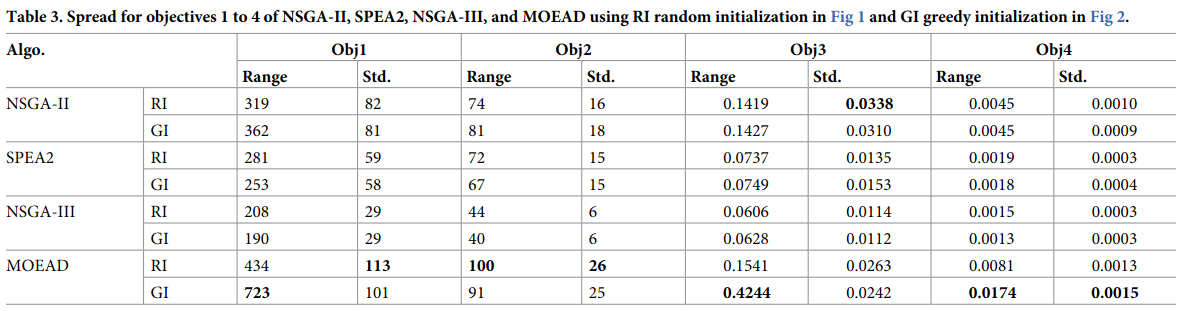
\includegraphics[width=0.9\textwidth]{analisis_assets/moqa_2022/tables/tabla_range_std.png}
    \caption{Captura de la Tabla 5 de Moqa et al. (2022). La demostración matemática del ratio ($8,08 > 2,83$) para el \textit{Avg Tolerance Rate} de NSGA-II (RI) confirma inequívocamente que \textit{Range} representa la media aritmética y no el rango estadístico.}
    \label{fig:moqa_errata_rango}
\end{figure}

\paragraph{Inconsistencias y Lagunas Críticas}
Más allá de las interpretaciones técnicas, el estudio de referencia adolece de una serie de omisiones críticas en su reporte que comprometen la integridad de la replicación. Estas lagunas no solo afectan a la configuración paramétrica de los algoritmos, sino que impactan directamente en la interpretación biológica de los resultados presentados:

\begin{itemize}
    \item \textbf{El Problema del Hipervolumen (HV):} Existe una falla de coherencia interna grave: los autores anuncian el HV como su métrica principal en el \textit{Abstract}, pero los resultados no aparecen en ninguna sección del cuerpo del documento. Además, se omite la declaración del punto de referencia (\textit{Reference Point}), lo que imposibilita cualquier comparación futura o validación de la calidad del frente de Pareto.
    \item \textbf{Indeterminación del Protocolo de Normalización:} El artículo indica explícitamente que \guillemotleft todos los objetivos son normalizados\guillemotright, pero omite por completo la fórmula matemática empleada (Z-score, Min-Max, Inversión, etc.). Esta carencia es crítica, pues la normalización no solo es un paso previo necesario para métricas como el Hipervolumen, sino que altera la topología del espacio de búsqueda y el comportamiento de los algoritmos de ordenamiento no dominado.
    \item \textbf{Crítica a la Trazabilidad y Relevancia Biológica:} Aunque el estudio es reproducible numéricamente gracias a la existencia de un archivo \texttt{input.txt}, carece de anclaje genómico real, es decir, de valor científico biológico. El manuscrito omite el número de cromosoma, las coordenadas exactas (ensamblajes GRCh37/38) y los identificadores rsID. Resulta especialmente problemático el reporte de que \textit{\guillemotleft Haplotype patterns are combined together to form one haplotype block\guillemotright} (pág. 9), lo que sugiere la creación de un bloque artificial mediante la mezcla de poblaciones (europeos, africanos y asiáticos). Dado que el Desequilibrio de Ligamiento (LD) es específico de cada población, esta práctica genera una estructura sintética que no existe en el genoma humano real, reduciendo el experimento a un ejercicio de optimización matemática sin validez biológica contrastable.
    \item \textbf{Ambigüedad Paramétrica en MOEA/D:} No se declara la función de agregación utilizada (Weighted Sum, PBI o Tchebycheff). En caso de haber usado PBI, se desconoce el parámetro de penalización ($\theta$), y para NSGA-III no se especifica el número de divisiones ($H$) que determina la densidad de los vectores de referencia.
    Por este motivo, en las ejecuciones A y B se evalúan de forma exhaustiva diferentes funciones de agregación para el algoritmo MOEA/D: 
    \begin{itemize}
        \item \textbf{WS (Weighted Sum):} Realiza una agregación lineal simple de los objetivos.
        \item \textbf{TCHE (Tchebycheff):} Minimiza la distancia de Tchebyshev respecto a un punto de referencia, permitiendo alcanzar soluciones en frentes no convexos.
        \item \textbf{PBI (Penalty-based Boundary Intersection):} Busca un equilibrio entre convergencia y diversidad mediante el ajuste del parámetro de penalización ($\theta$).
    \end{itemize}
\end{itemize}



Esta falta de transparencia refuerza la importancia de la implementación propia desarrollada en este trabajo, la cual garantiza una especificación completa de parámetros y una semántica de métricas rigurosa.

\subsection{Resultados y análisis (Moqa 2022)}
\label{sec:res_analisis_moqa}

\subsubsection{Frentes de Pareto}
En esta sección se presentan los frentes de Pareto reportados por Moqa et al. (2022), contrastando el desempeño de los algoritmos bajo inicialización aleatoria (RI) y heurística (GI).

\begin{figure}[H]
    \centering
    \begin{subfigure}[b]{0.45\textwidth}
        \centering
        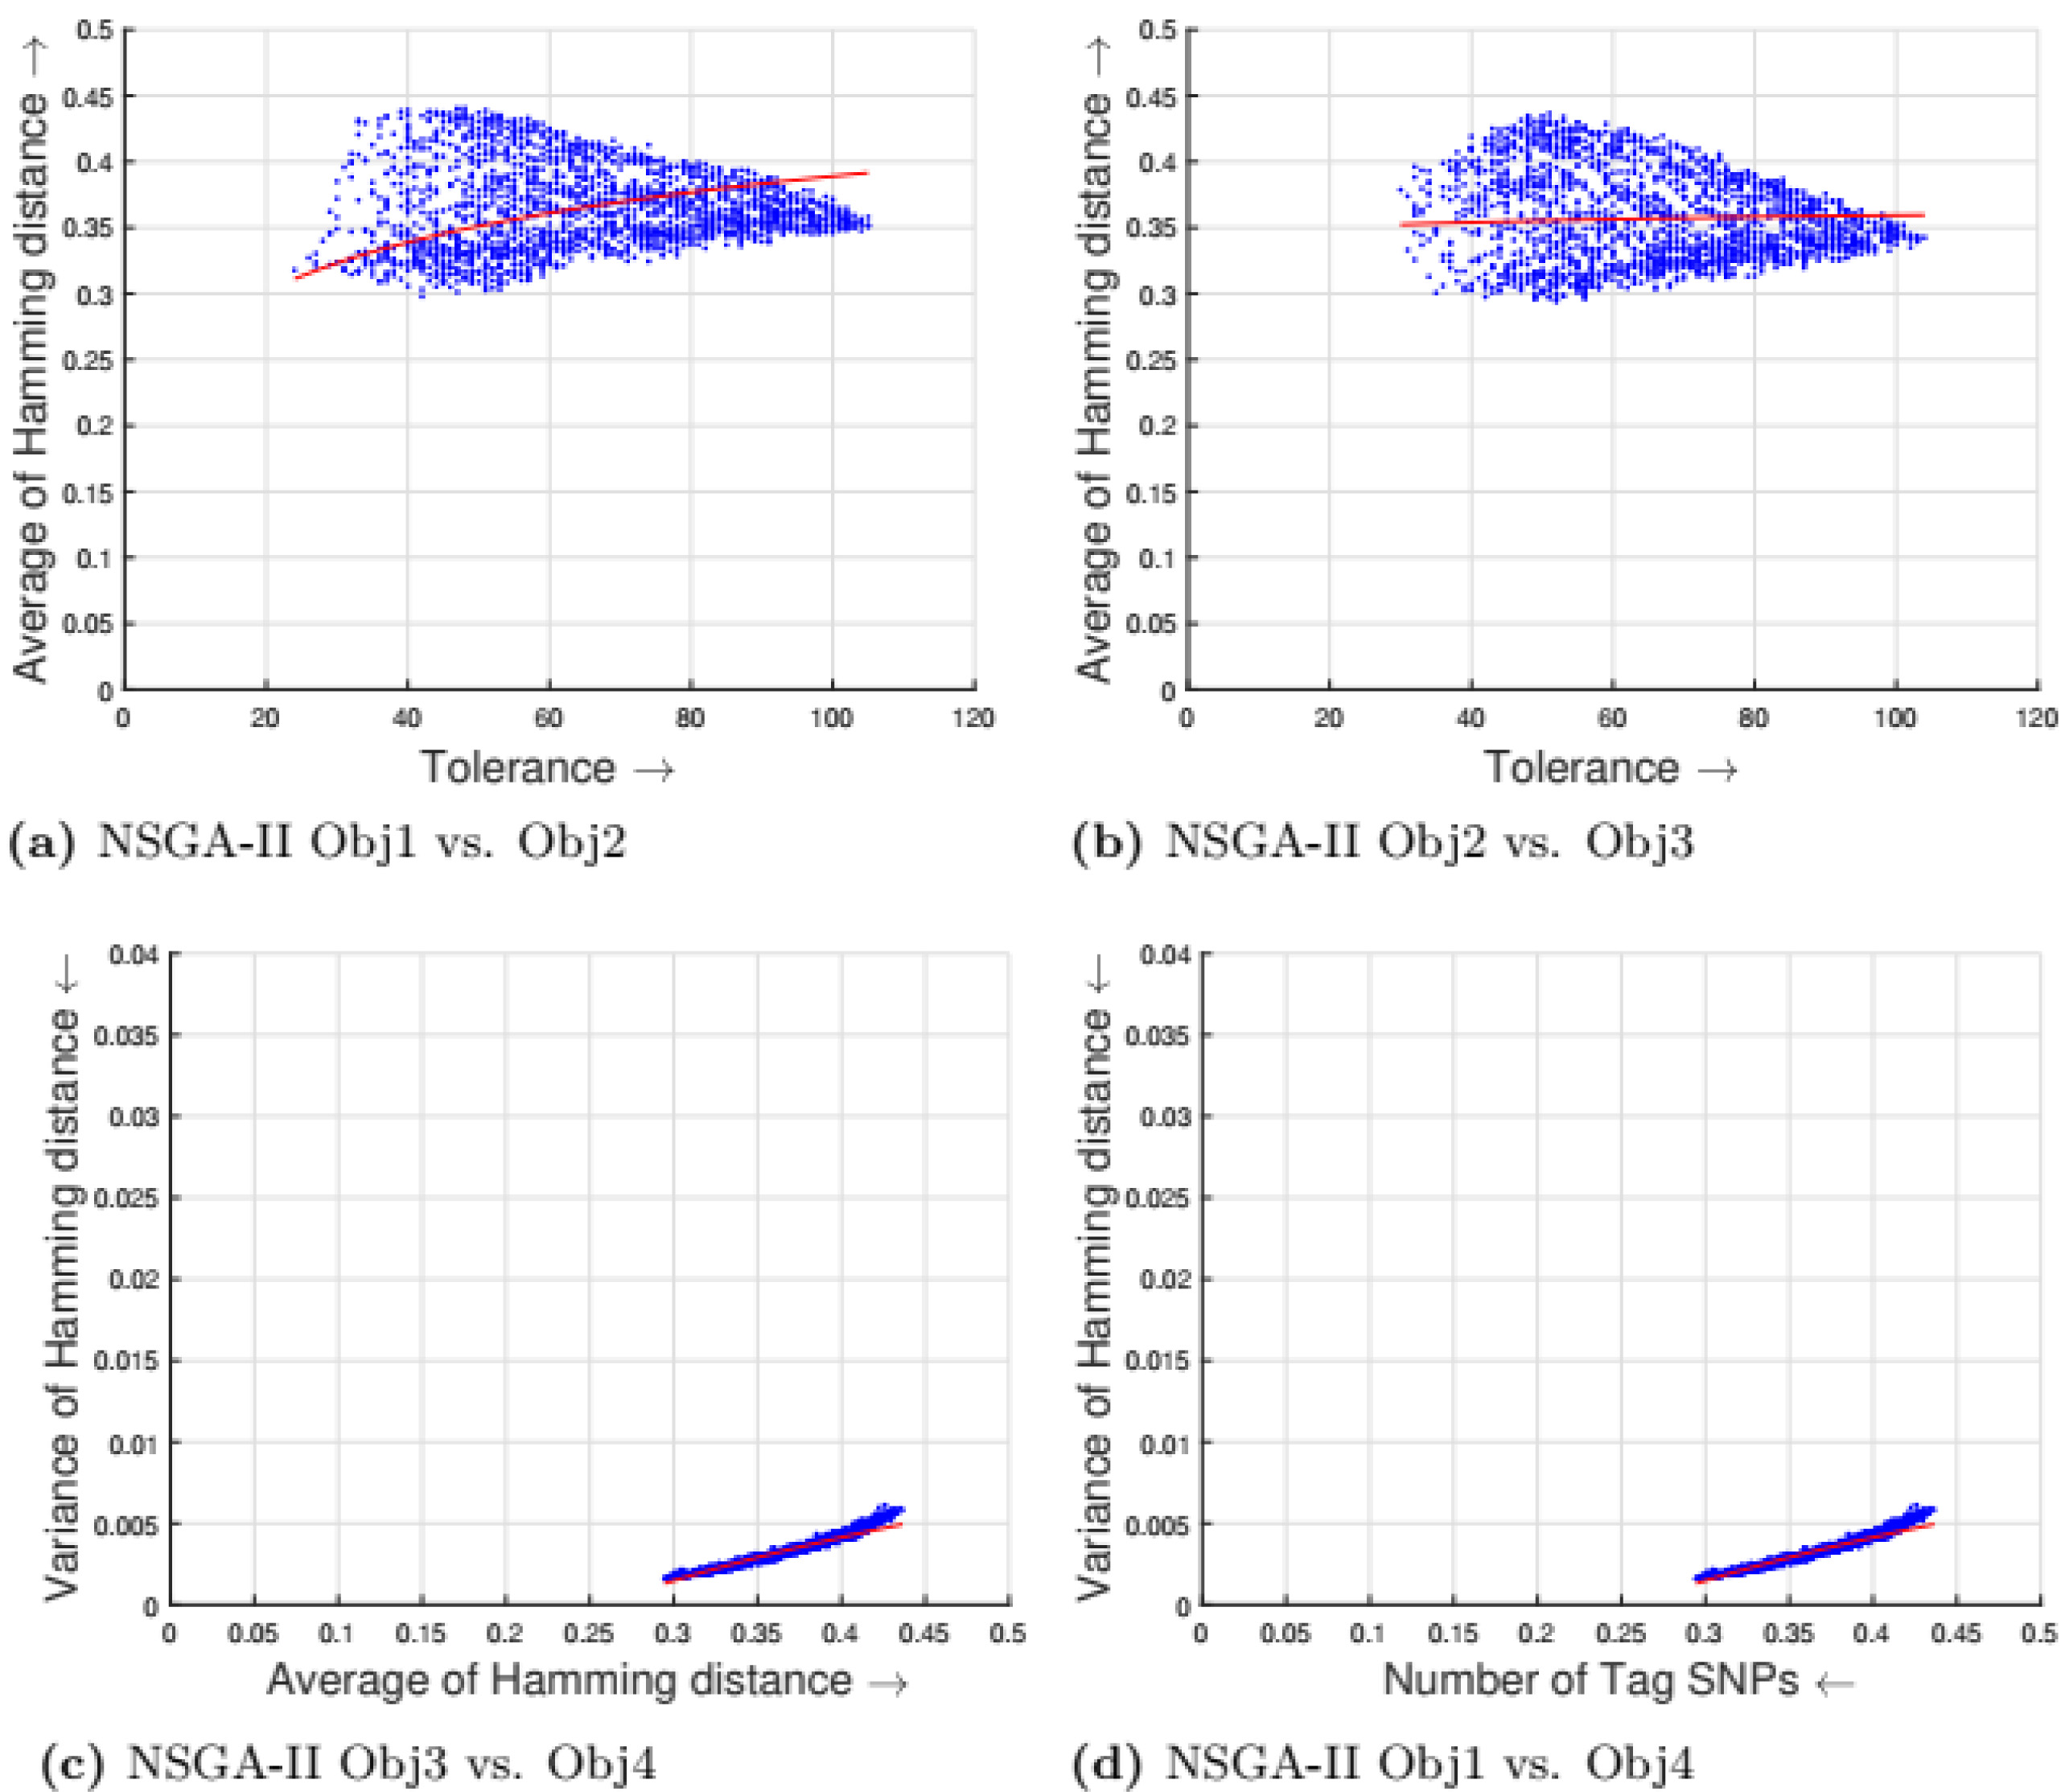
\includegraphics[width=\textwidth]{analisis_assets/moqa_2022/figures/moqa_fig_nsga2_random.jpeg}
        \caption{NSGA-II (RI)}
    \end{subfigure}
    \hfill
    \begin{subfigure}[b]{0.45\textwidth}
        \centering
        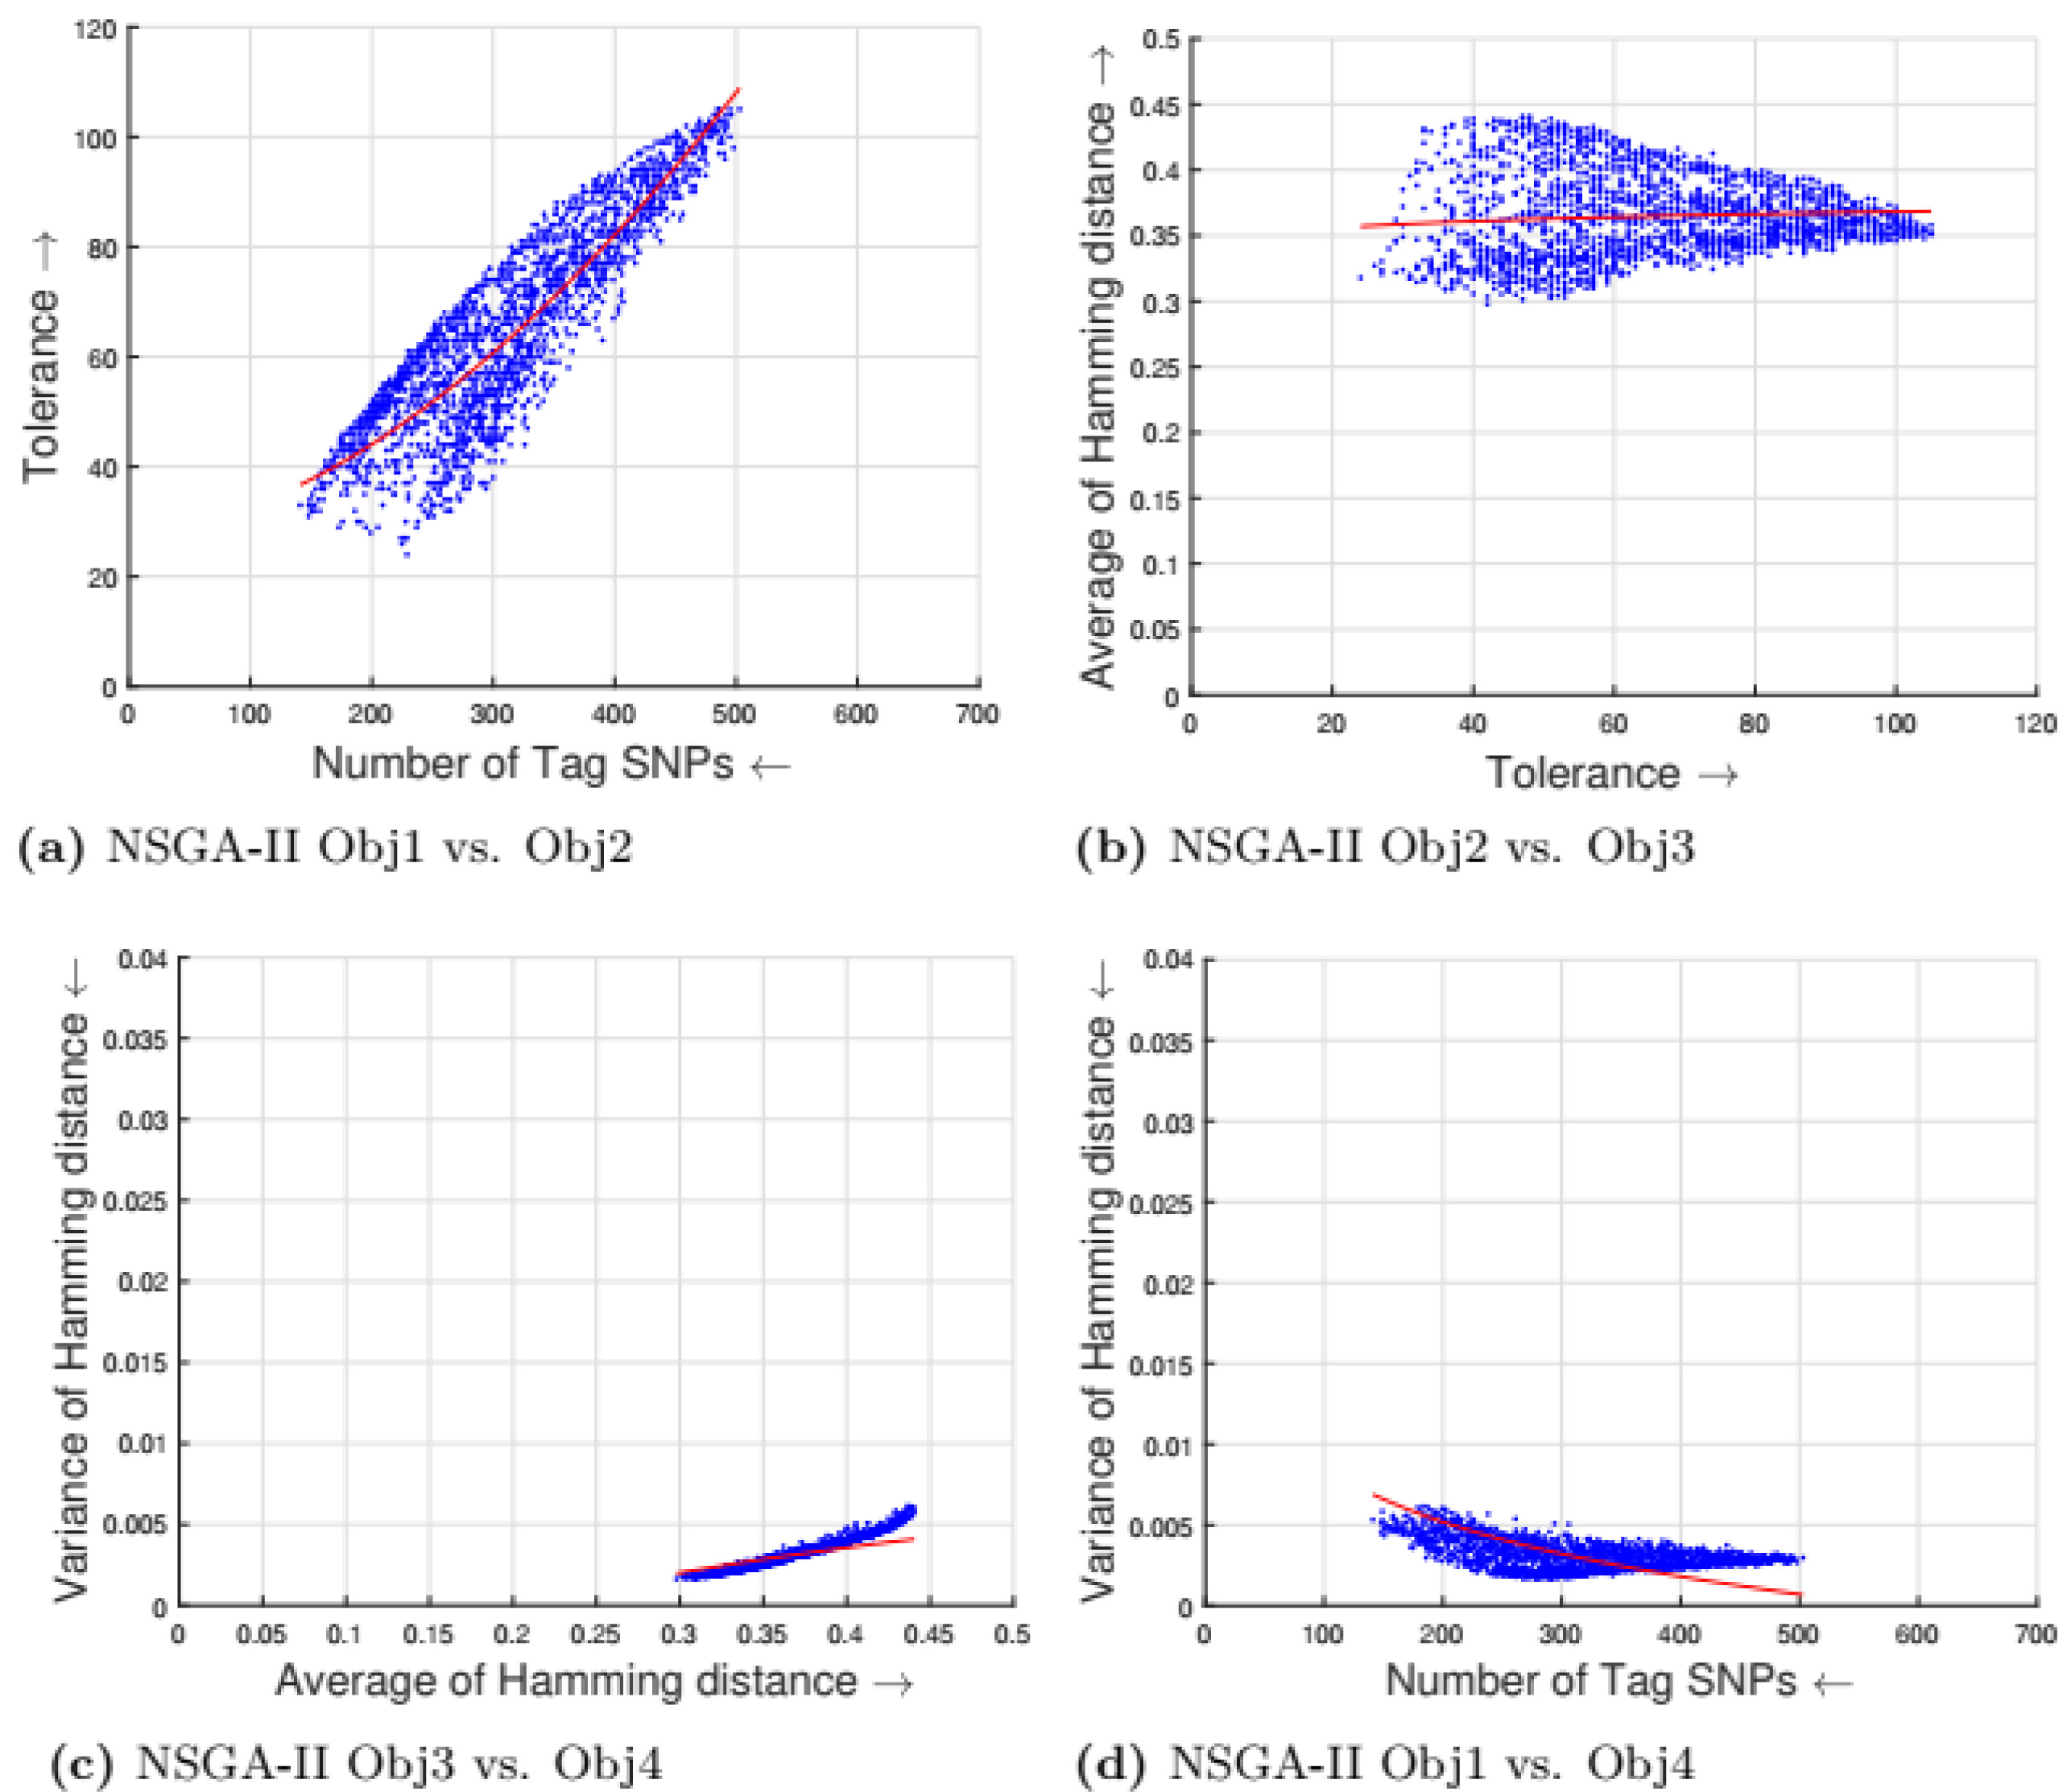
\includegraphics[width=\textwidth]{analisis_assets/moqa_2022/figures/moqa_fig_nsga2_greedy.jpeg}
        \caption{NSGA-II (GI)}
    \end{subfigure}
    \vskip\baselineskip
    \begin{subfigure}[b]{0.45\textwidth}
        \centering
        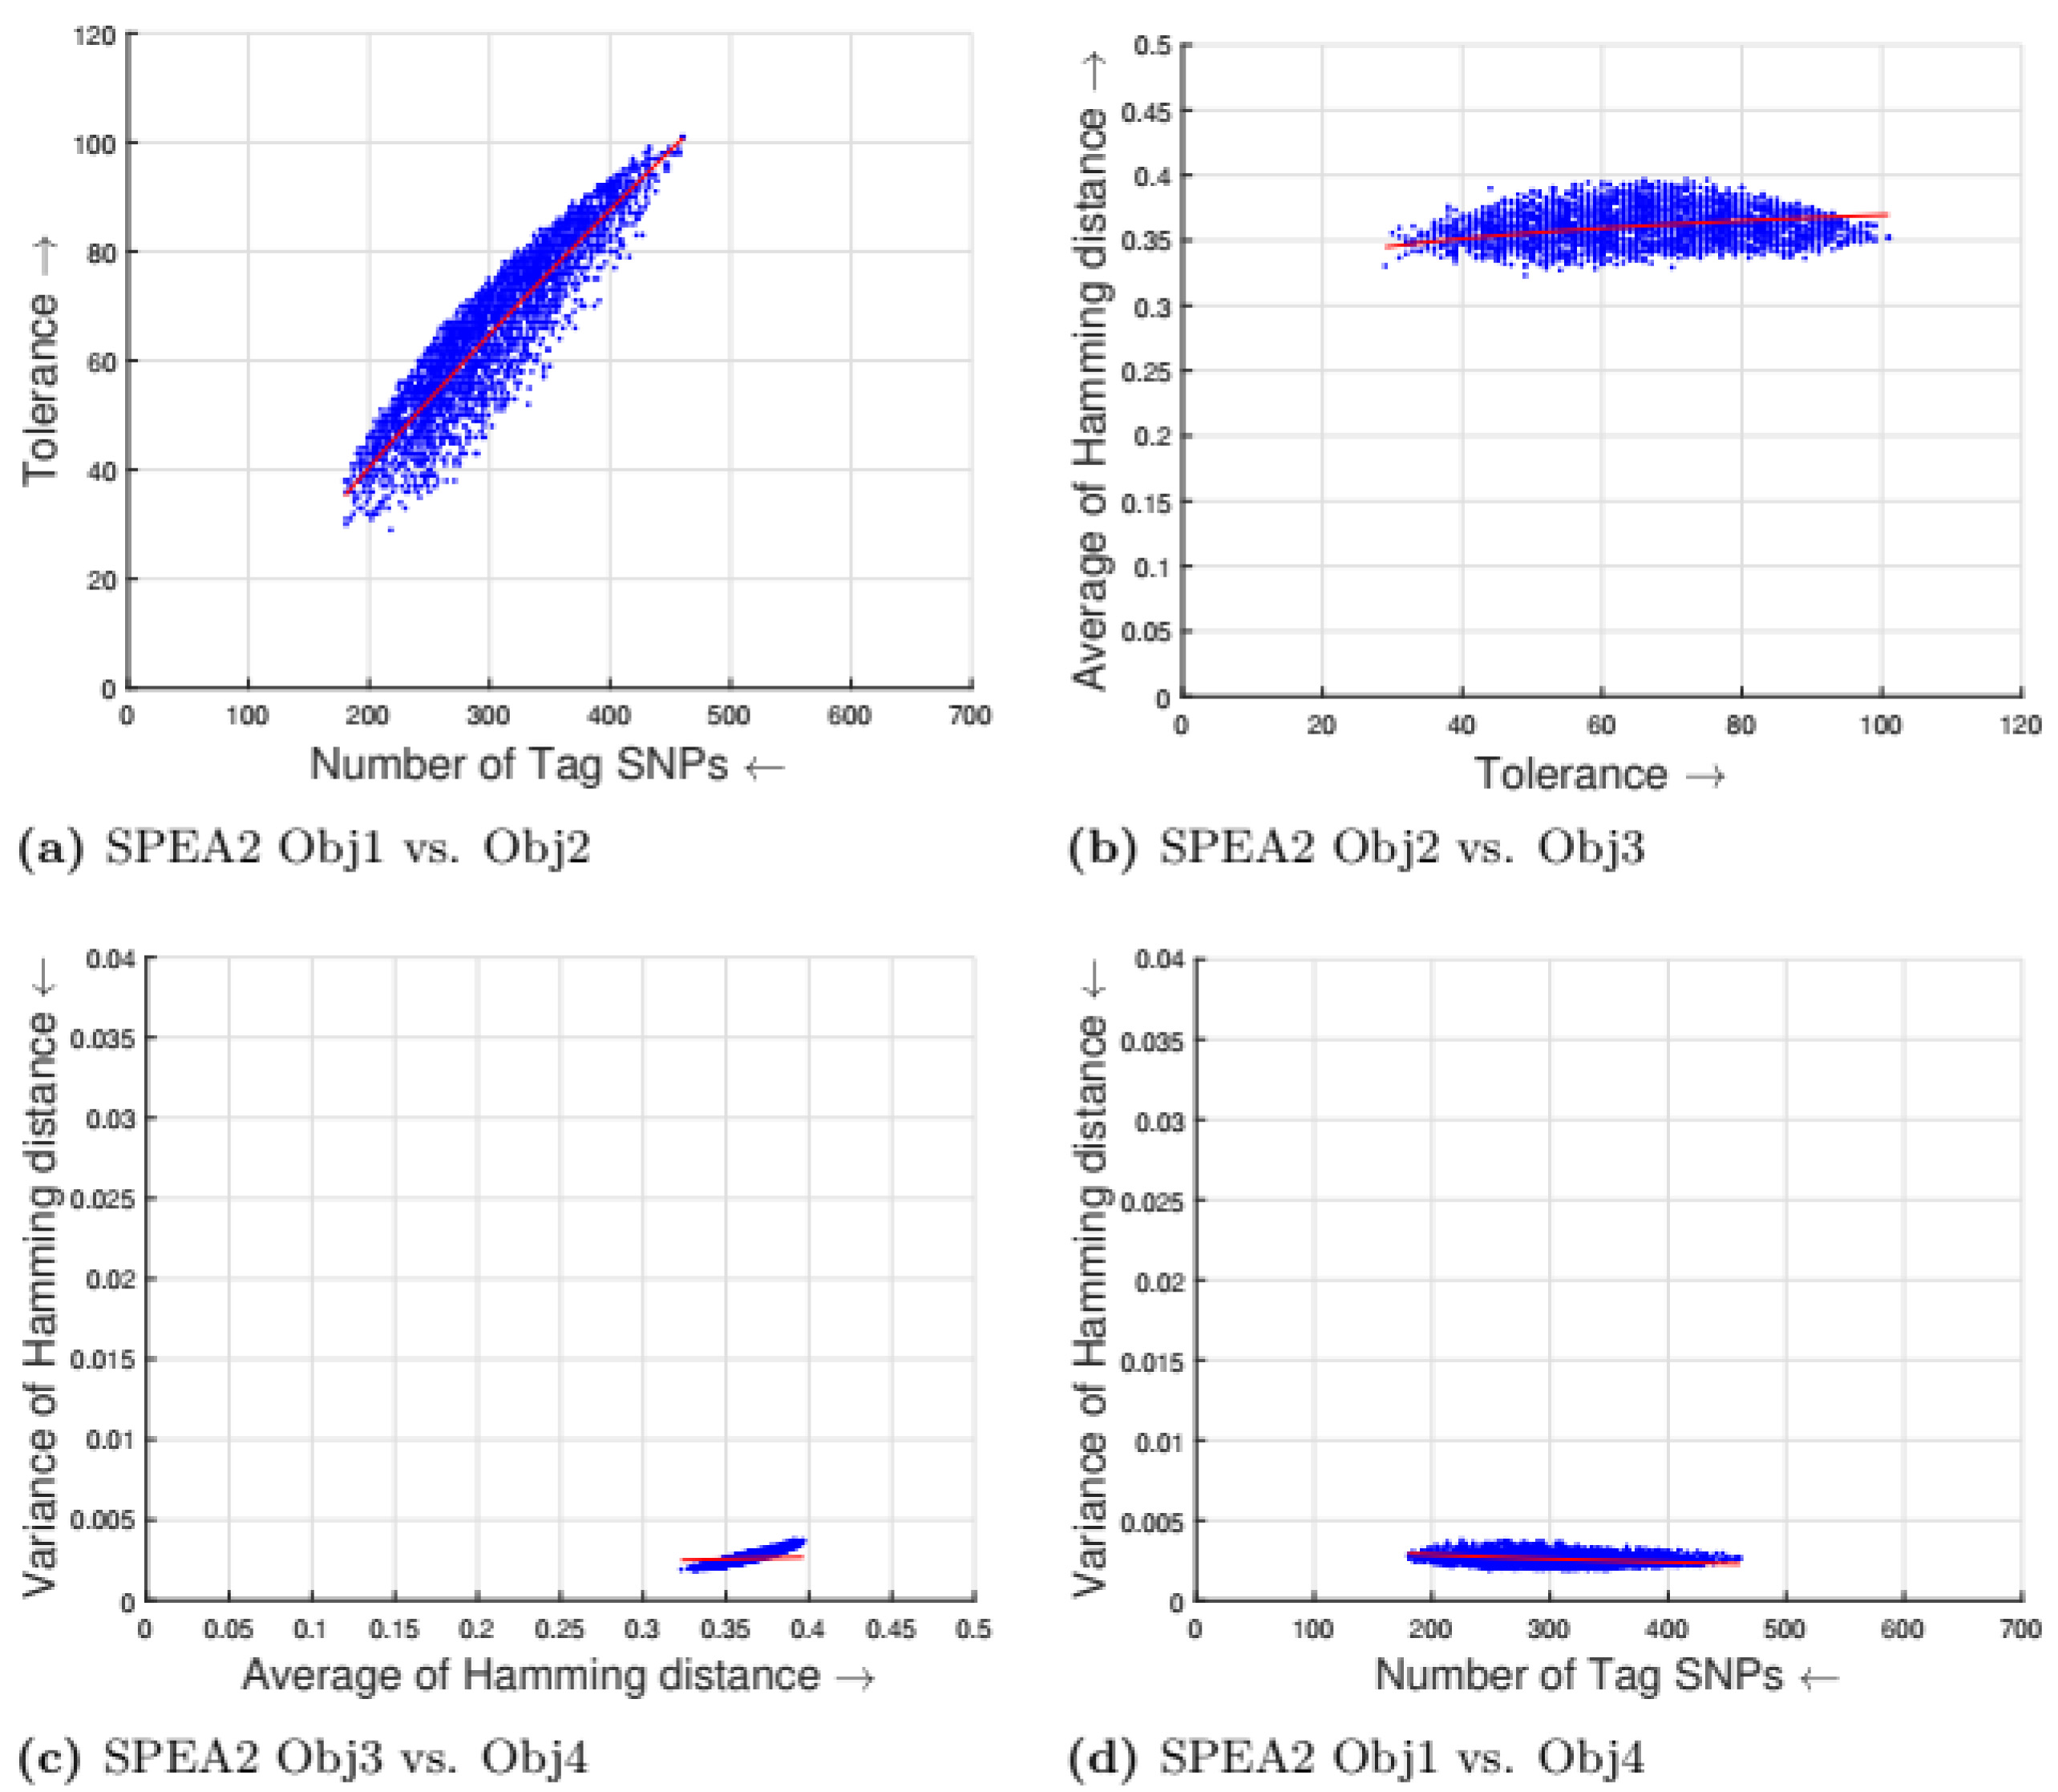
\includegraphics[width=\textwidth]{analisis_assets/moqa_2022/figures/moqa_fig_spea2_random.jpeg}
        \caption{SPEA2 (RI)}
    \end{subfigure}
    \hfill
    \begin{subfigure}[b]{0.45\textwidth}
        \centering
        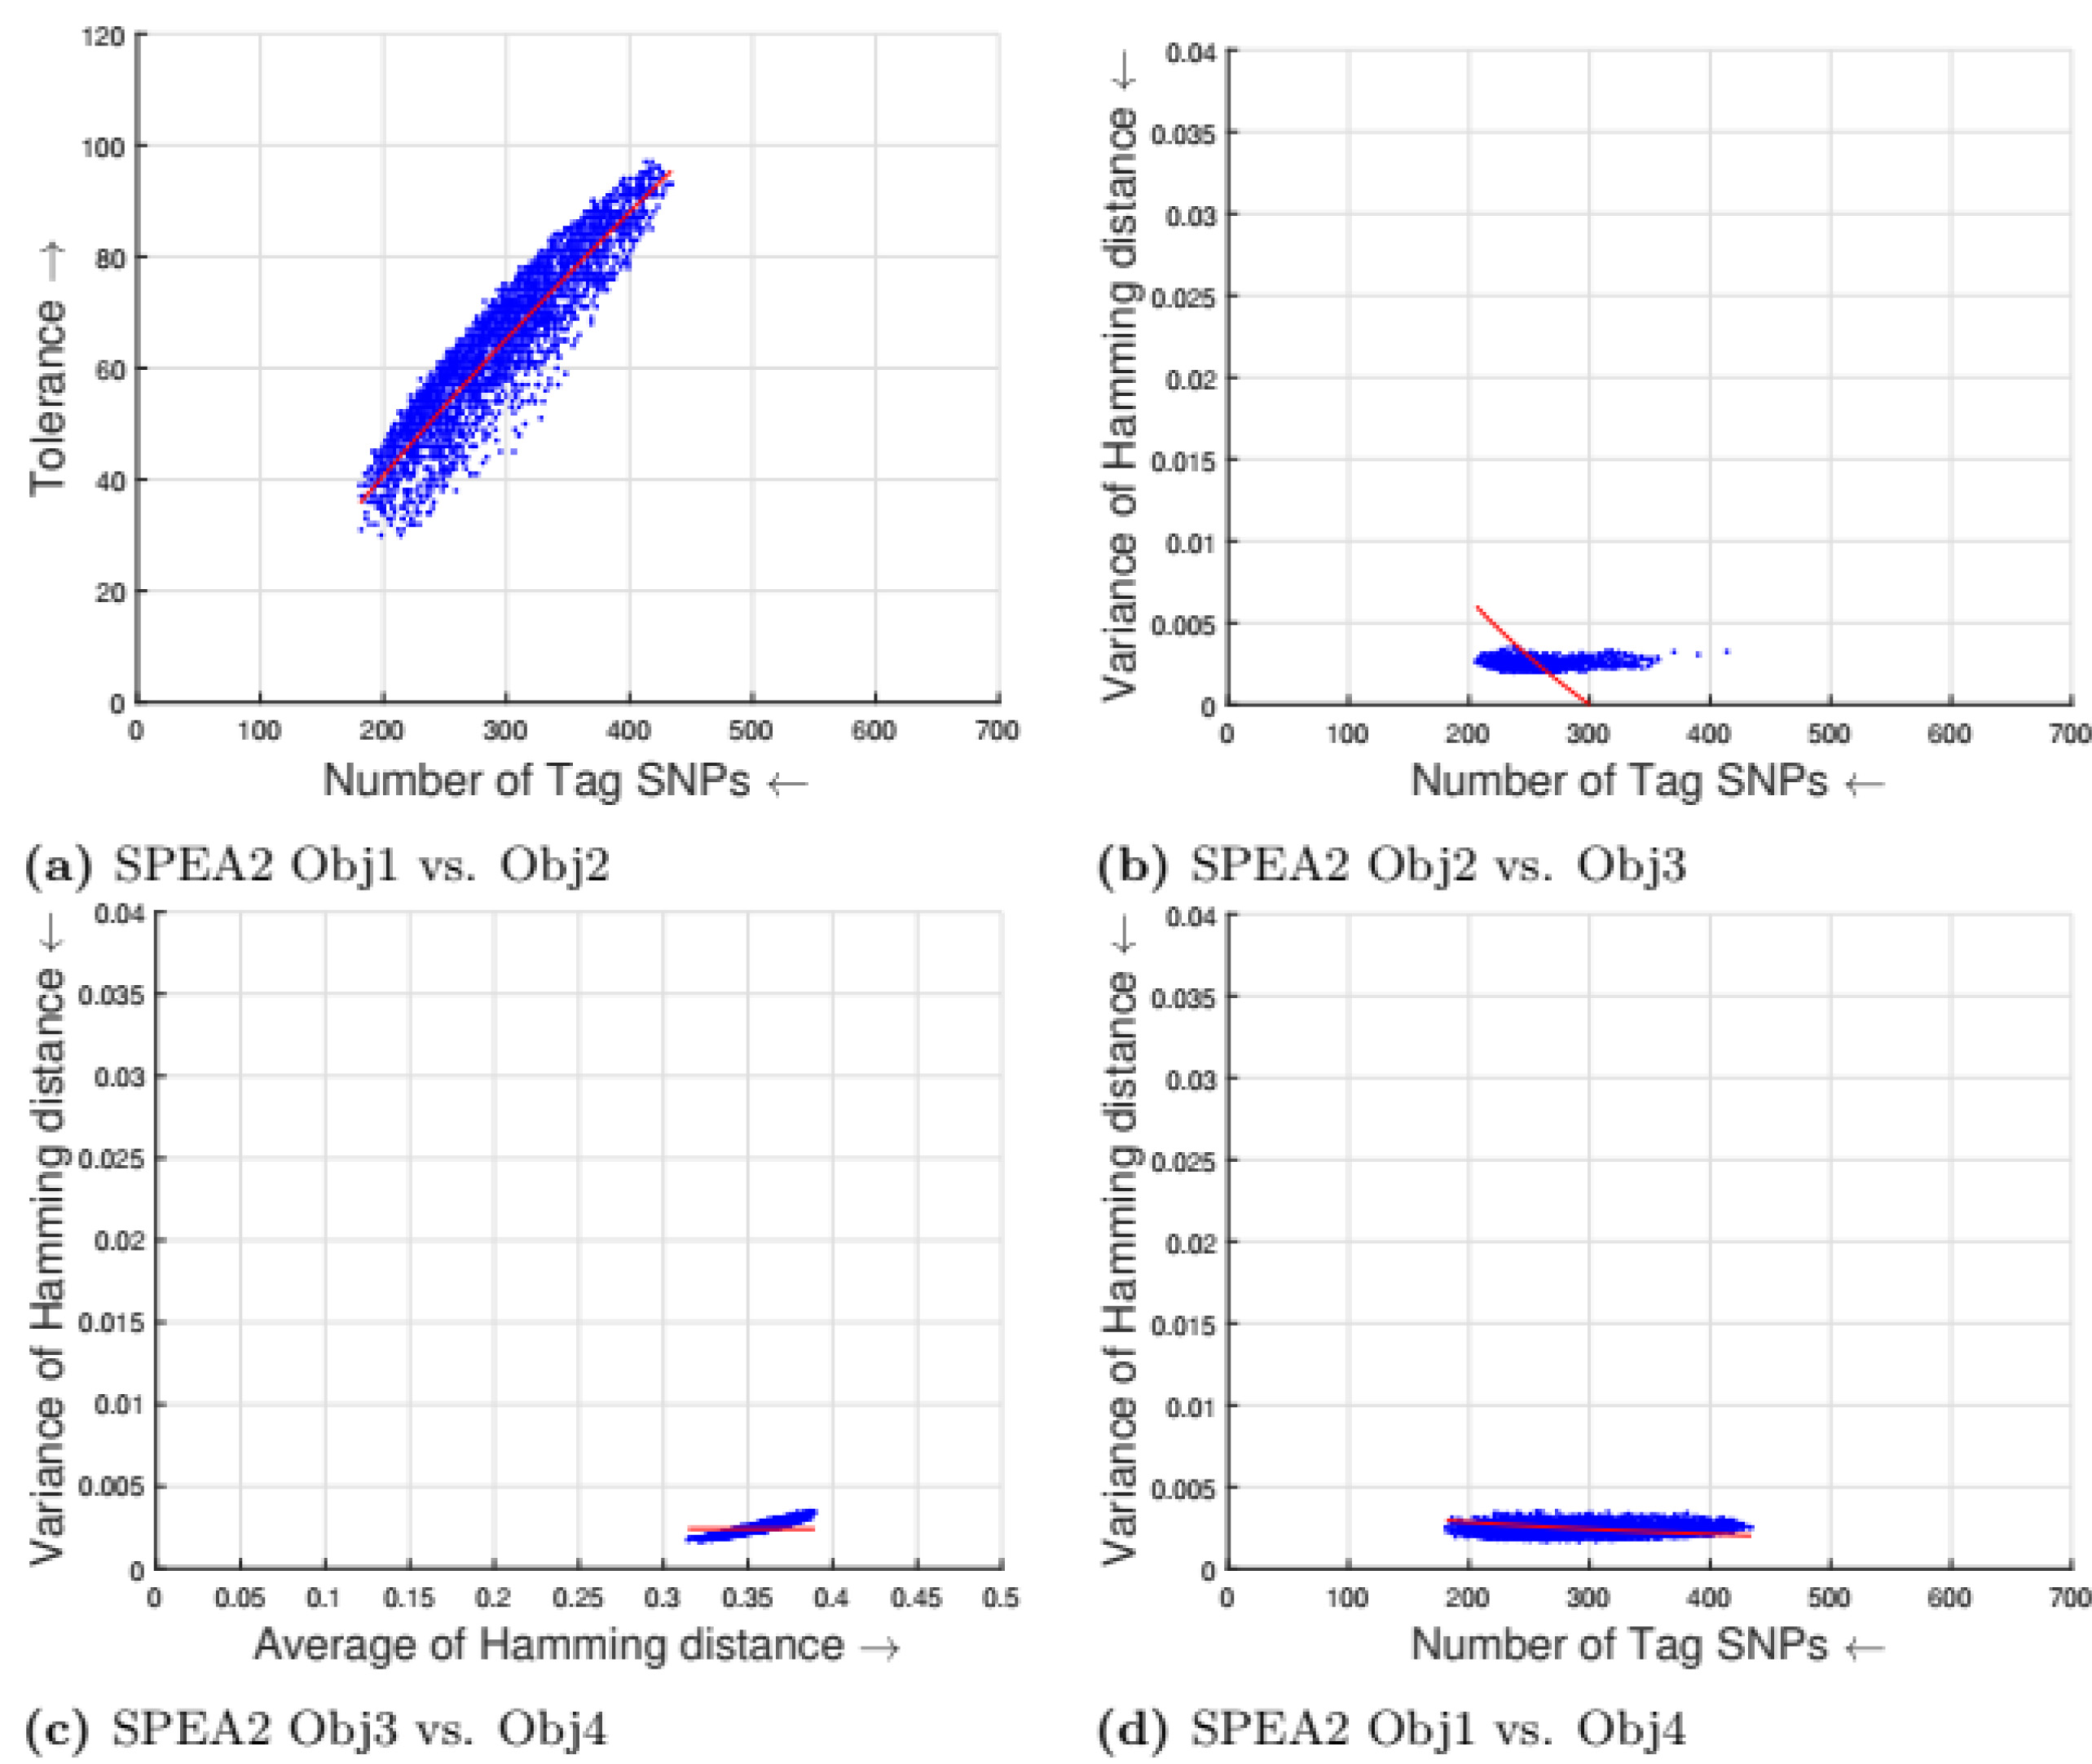
\includegraphics[width=\textwidth]{analisis_assets/moqa_2022/figures/moqa_fig_spea2_greedy.jpeg}
        \caption{SPEA2 (GI)}
    \end{subfigure}
    \caption{Comparativa de Frentes de Pareto: NSGA-II y SPEA2 (Moqa 2022).}
\end{figure}

\begin{figure}[H]
    \centering
    \begin{subfigure}[b]{0.45\textwidth}
        \centering
        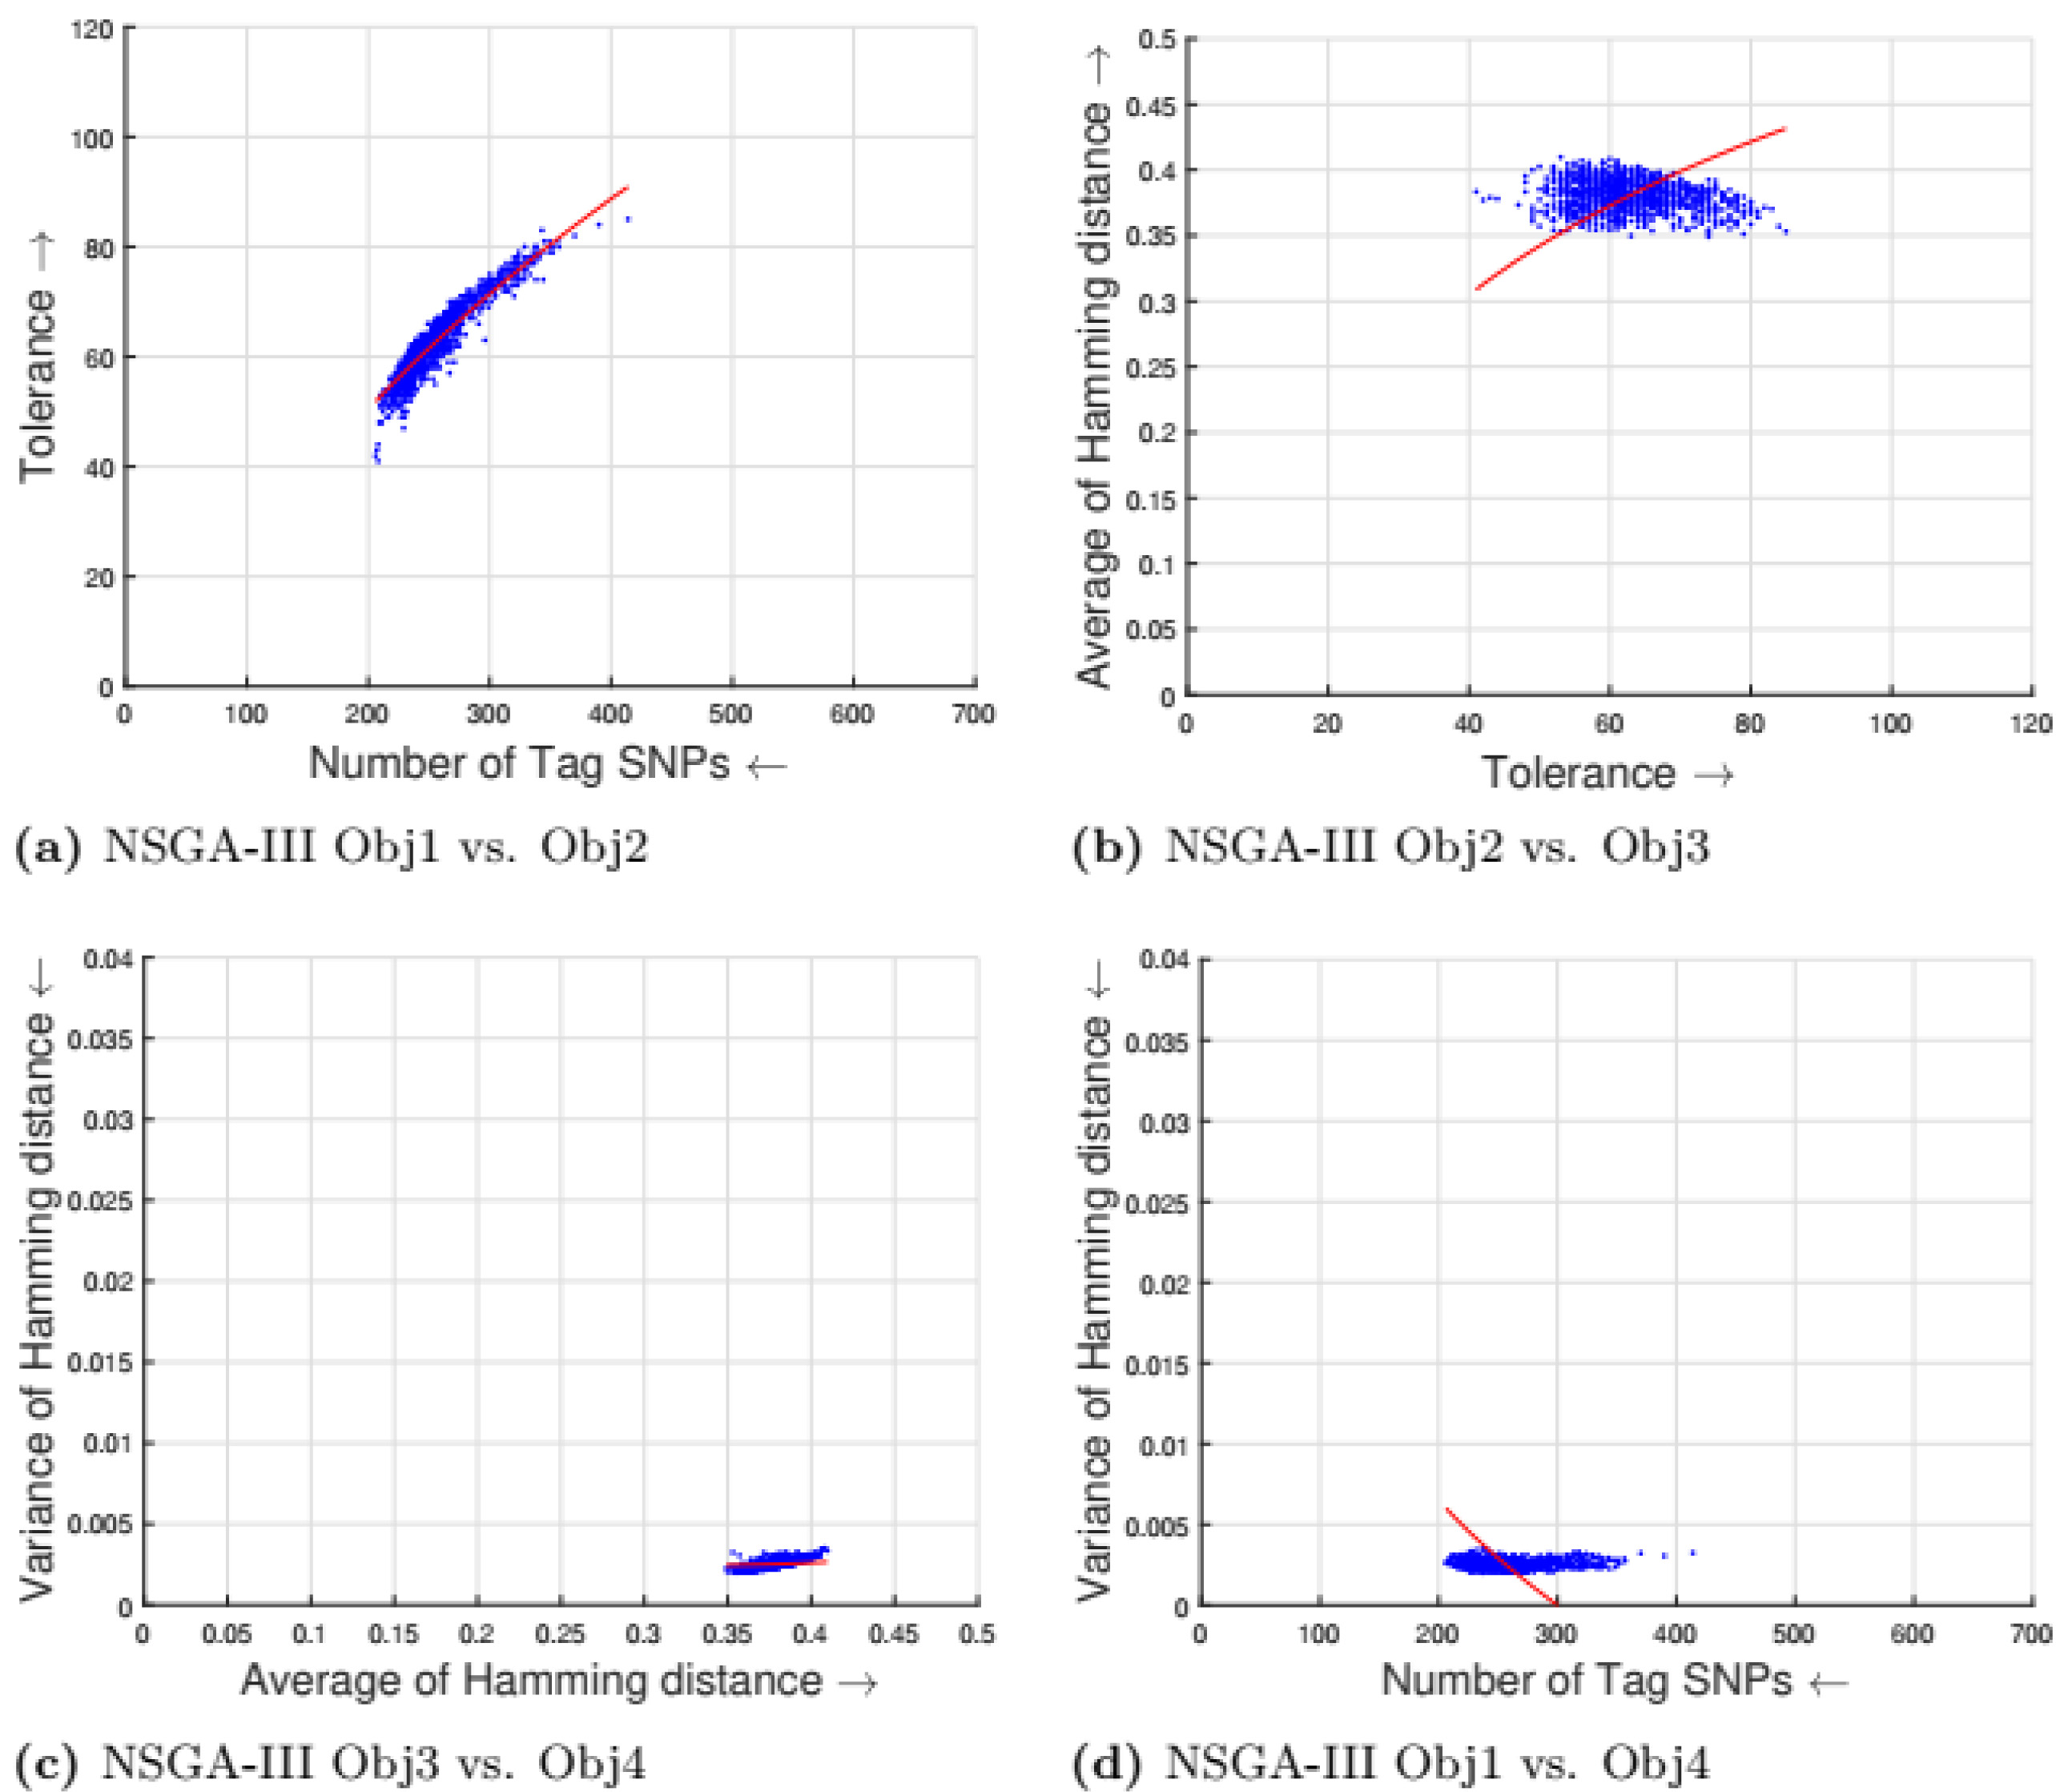
\includegraphics[width=\textwidth]{analisis_assets/moqa_2022/figures/moqa_fig_nsga3_random.jpeg}
        \caption{NSGA-III (RI)}
    \end{subfigure}
    \hfill
    \begin{subfigure}[b]{0.45\textwidth}
        \centering
        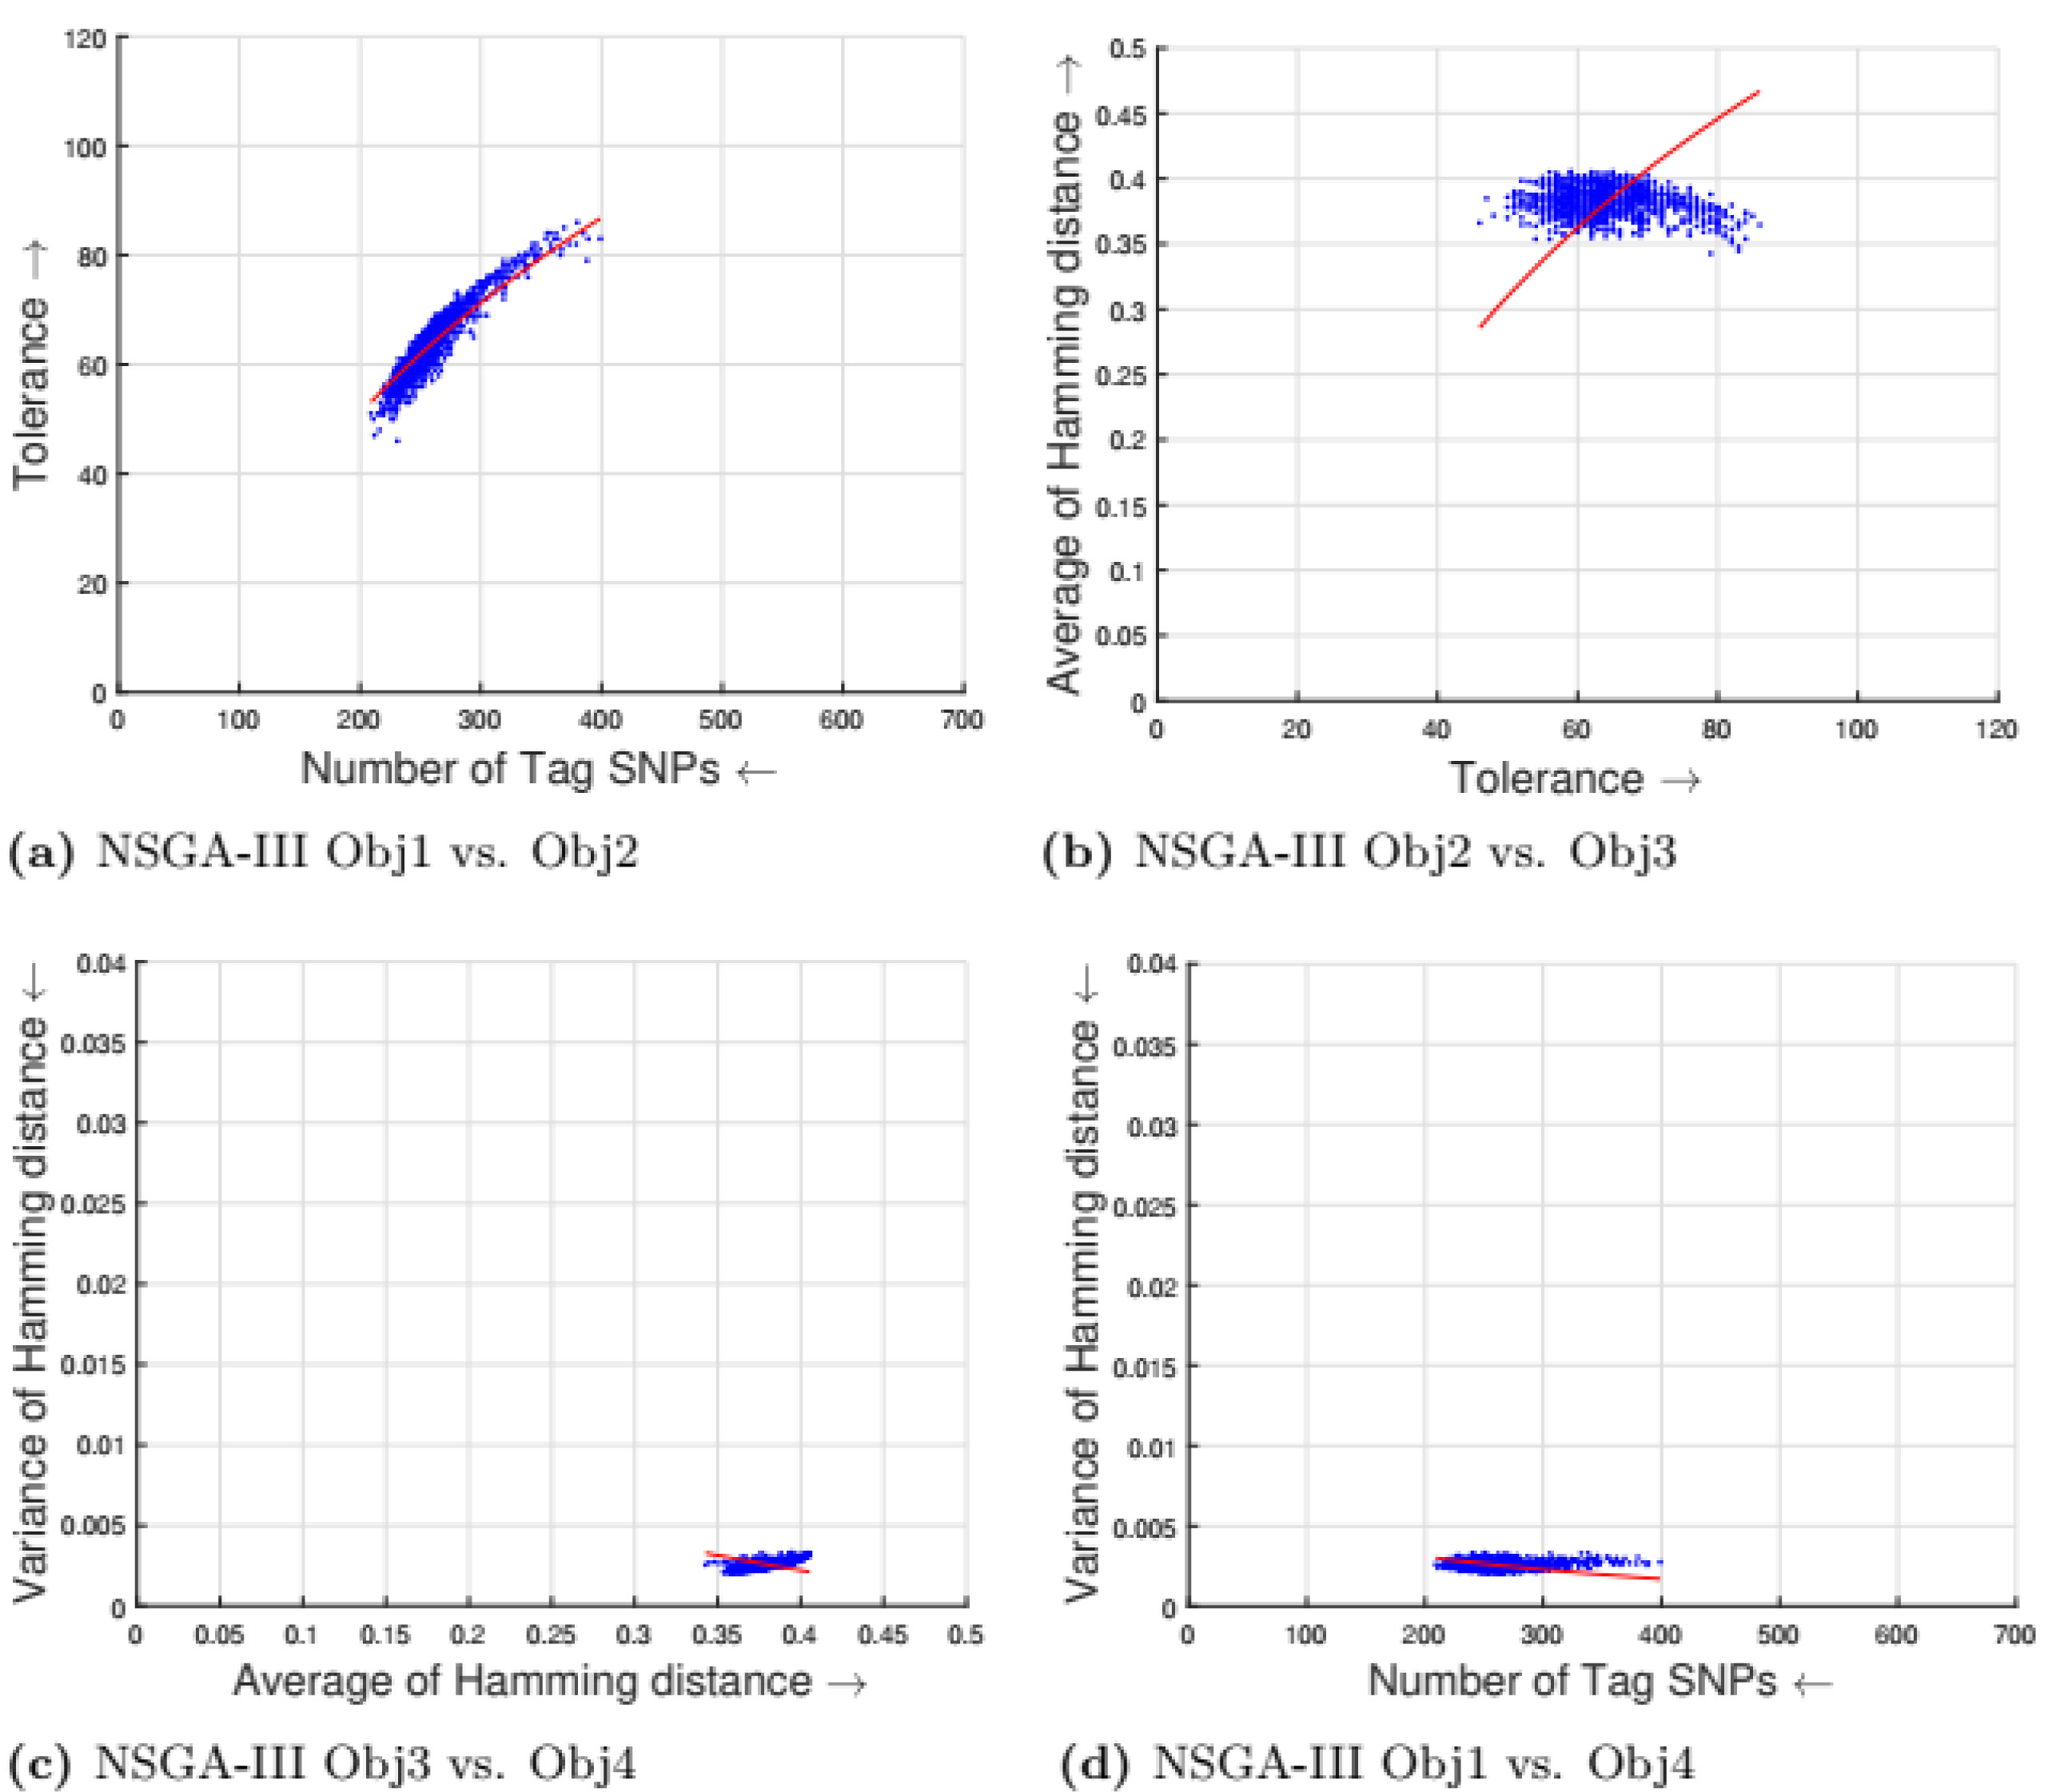
\includegraphics[width=\textwidth]{analisis_assets/moqa_2022/figures/moqa_fig_nsga3_greedy.jpeg}
        \caption{NSGA-III (GI)}
    \end{subfigure}
    \vskip\baselineskip
    \begin{subfigure}[b]{0.45\textwidth}
        \centering
        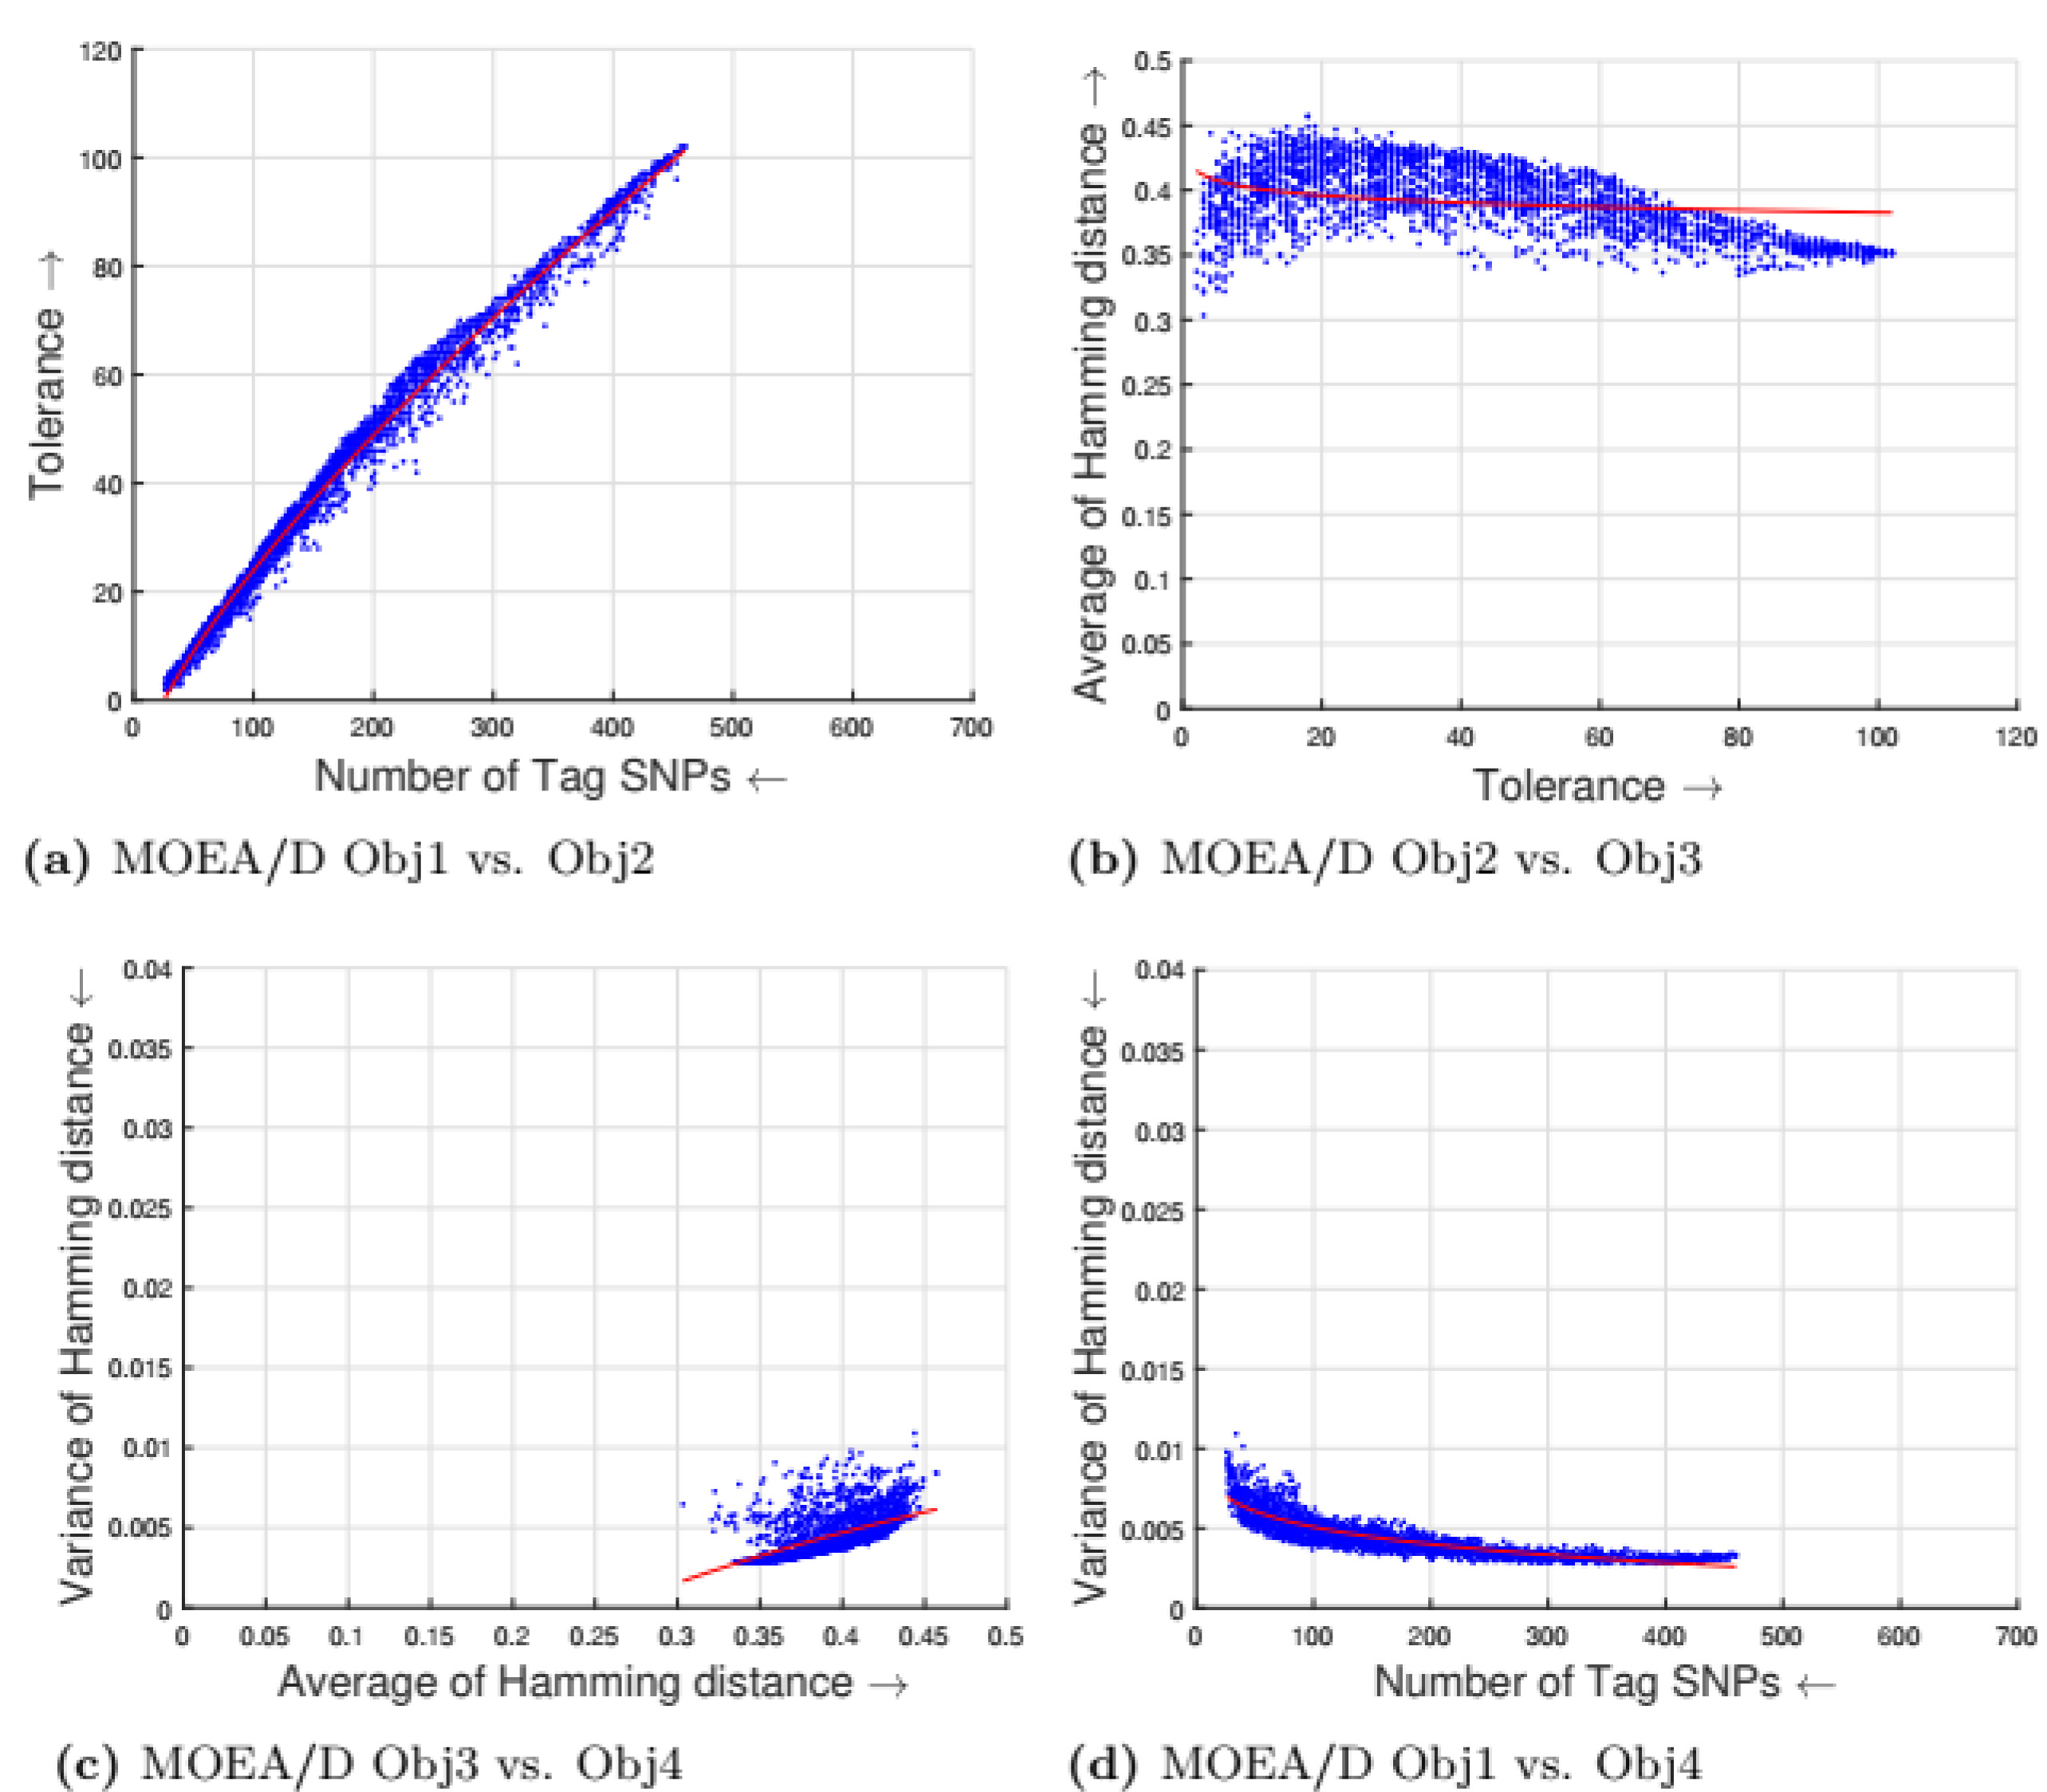
\includegraphics[width=\textwidth]{analisis_assets/moqa_2022/figures/moqa_fig_moead_random.jpeg}
        \caption{MOEA/D (RI)}
    \end{subfigure}
    \hfill
    \begin{subfigure}[b]{0.45\textwidth}
        \centering
        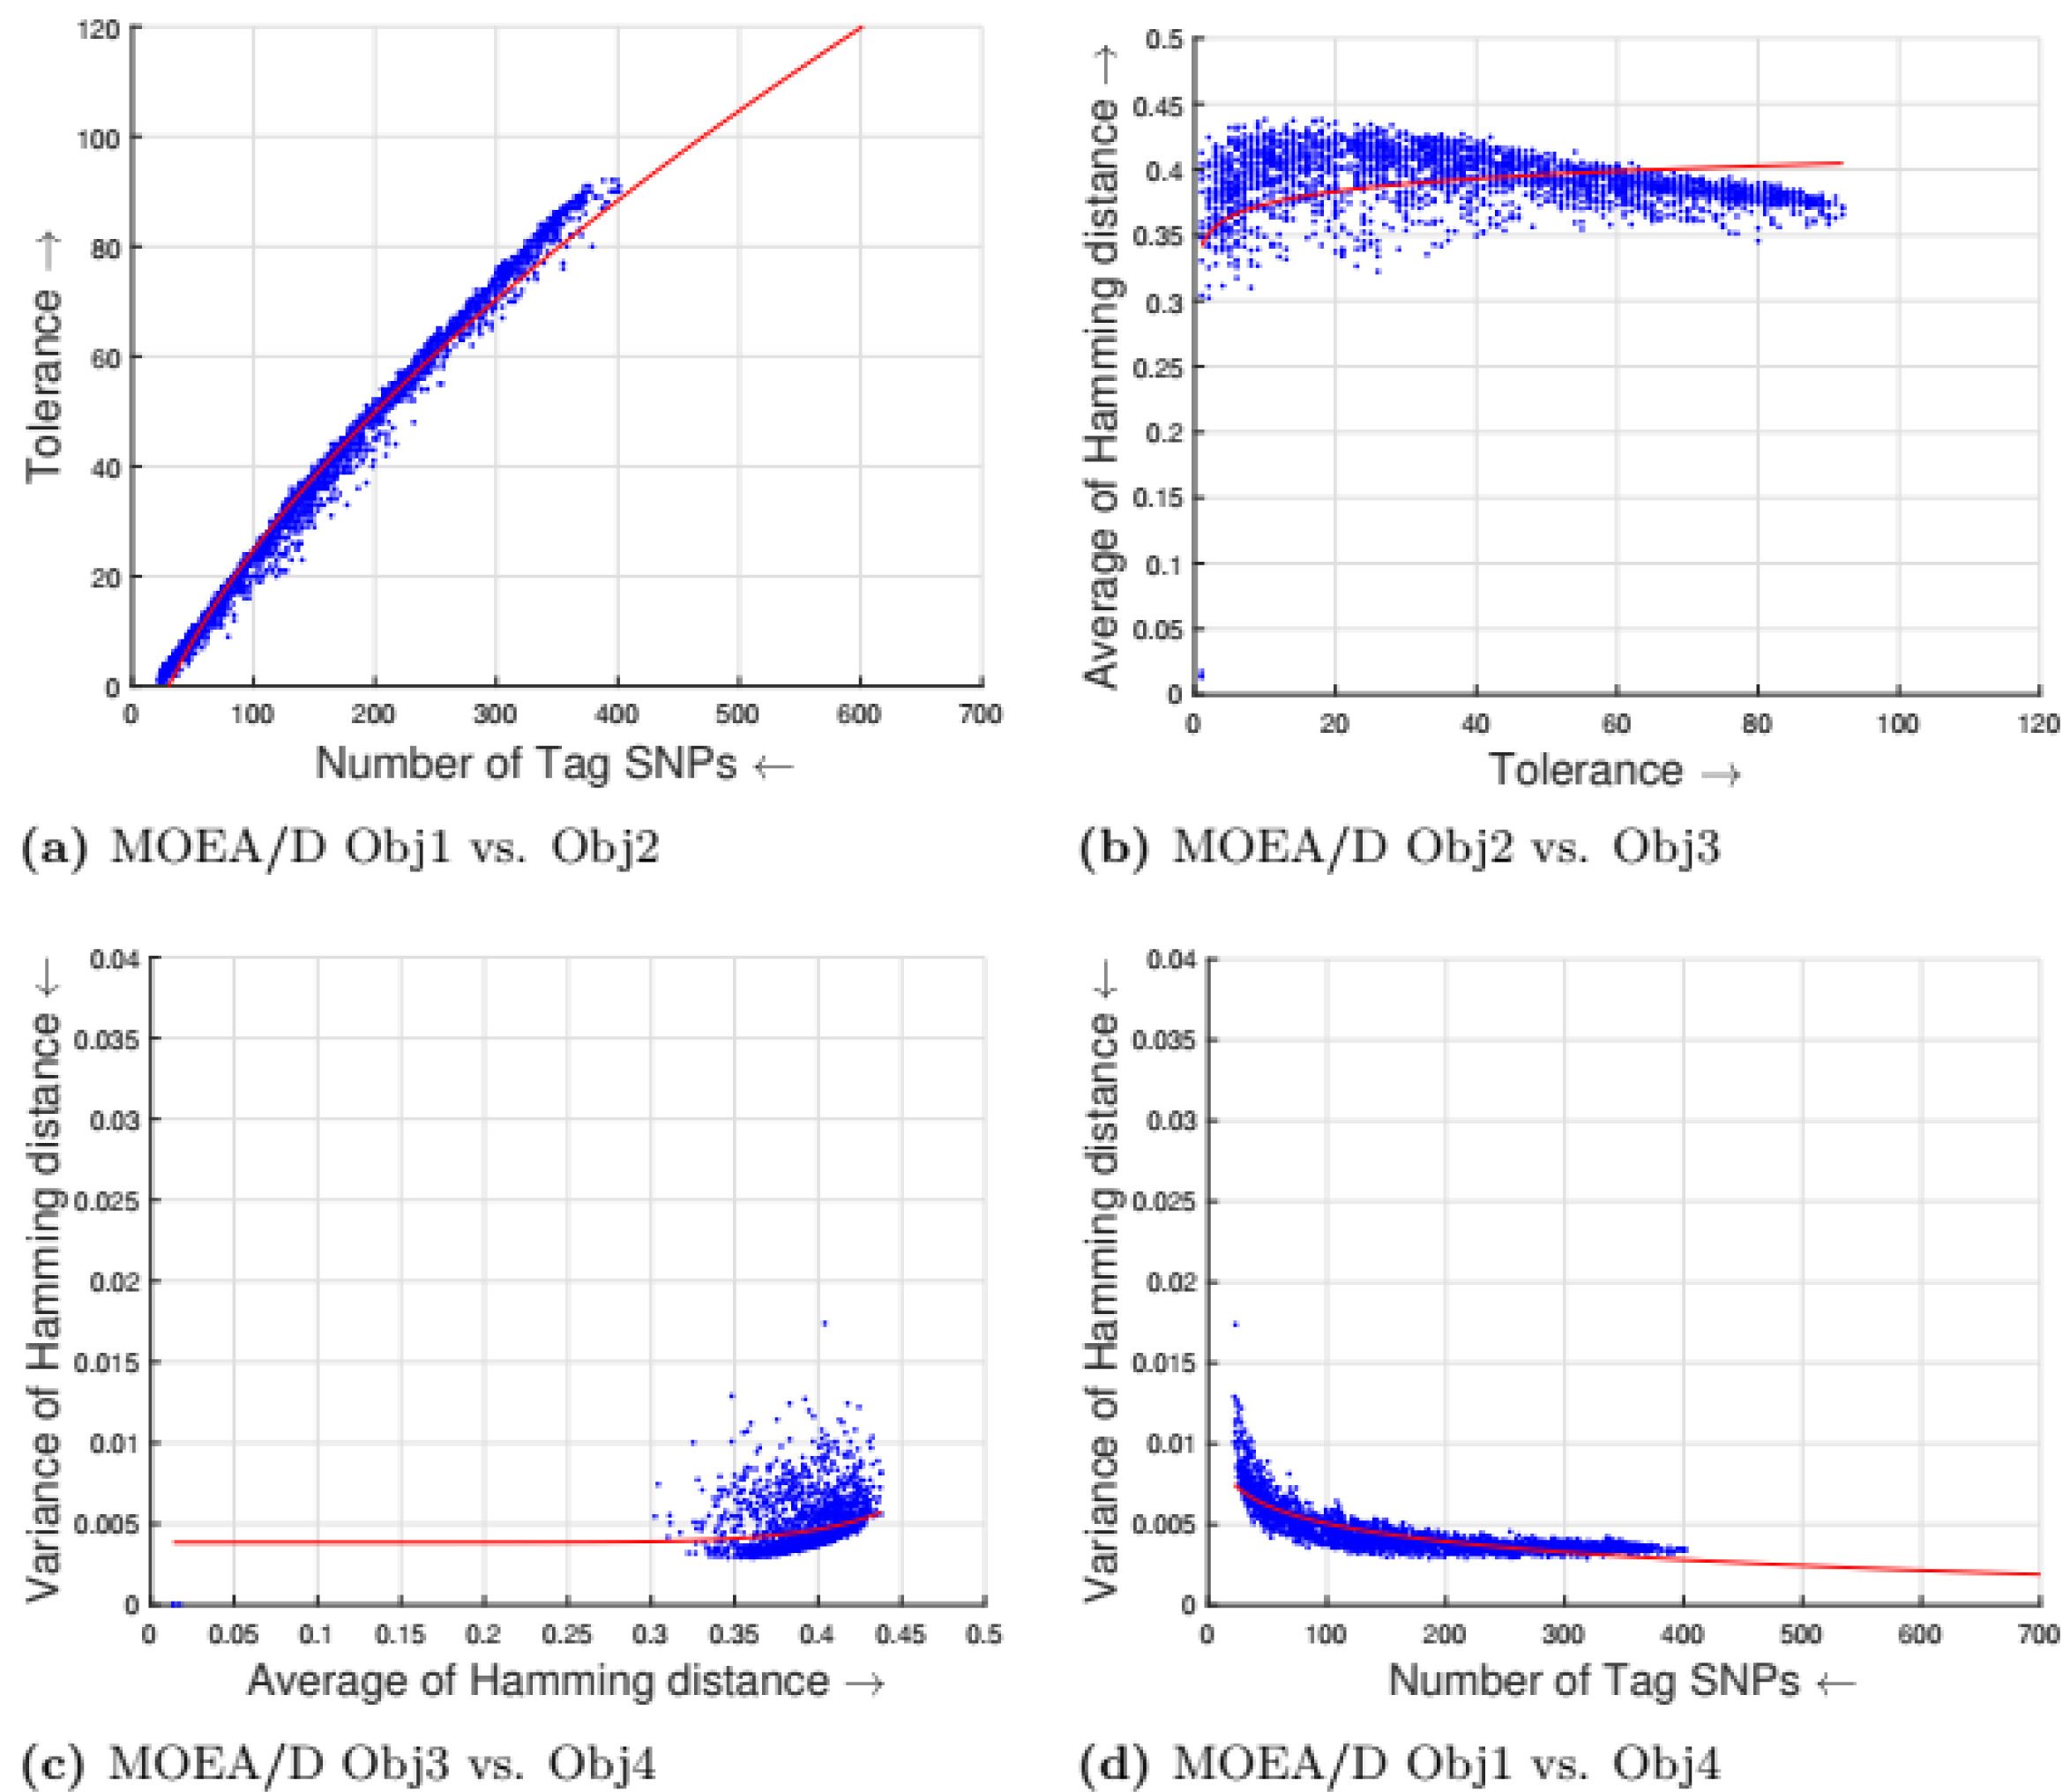
\includegraphics[width=\textwidth]{analisis_assets/moqa_2022/figures/moqa_fig_moead_greedy.jpeg}
        \caption{MOEA/D (GI)}
    \end{subfigure}
    \caption{Comparativa de Frentes de Pareto: NSGA-III y MOEA/D (Moqa 2022).}
\end{figure}

\subsubsection{Convergencia progresiva}
\begin{figure}[H]
    \centering
    \begin{subfigure}[b]{0.48\textwidth}
        \centering
        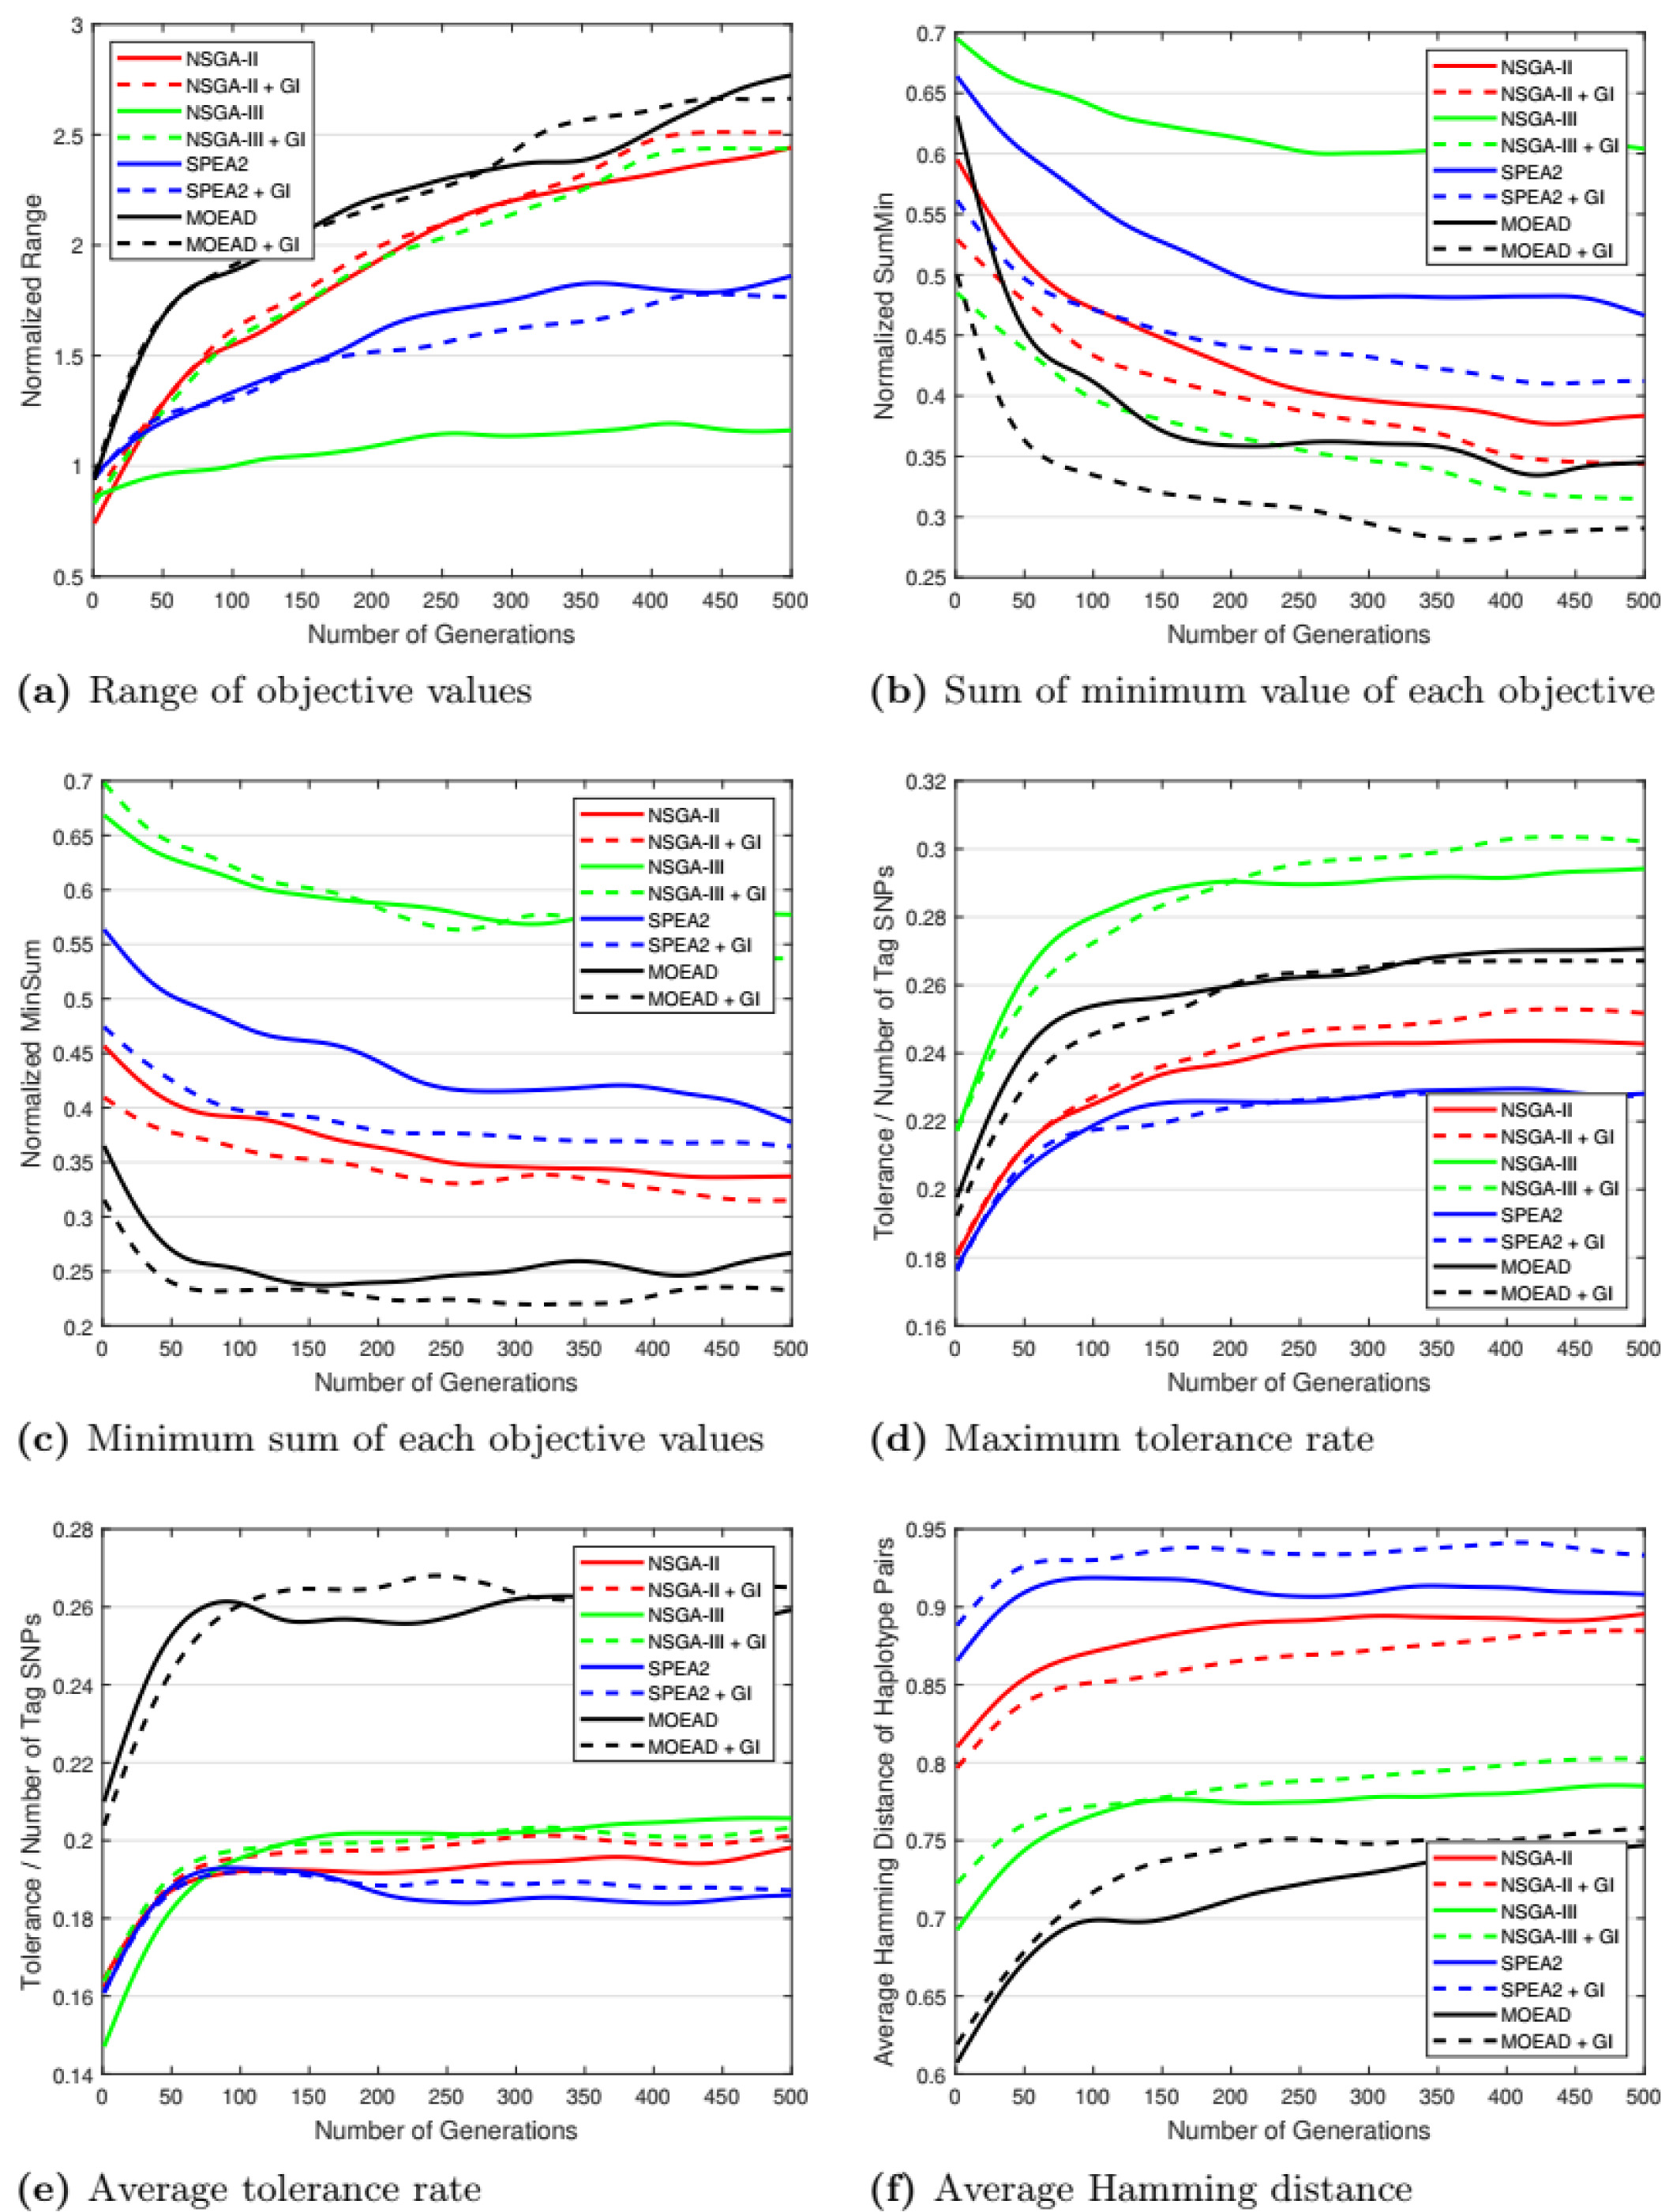
\includegraphics[width=\textwidth]{analisis_assets/moqa_2022/figures/moqa_fig_convergencia_1.jpeg}
        \caption{Evolución por generación de seis métricas de rendimiento en el experimento base (500 generaciones, población = 200). Se ilustra el impacto de la inicialización heurística (GI, líneas discontinuas) frente a la aleatoria (RI, líneas continuas).}
    \end{subfigure}
    \hfill
    \begin{subfigure}[b]{0.48\textwidth}
        \centering
        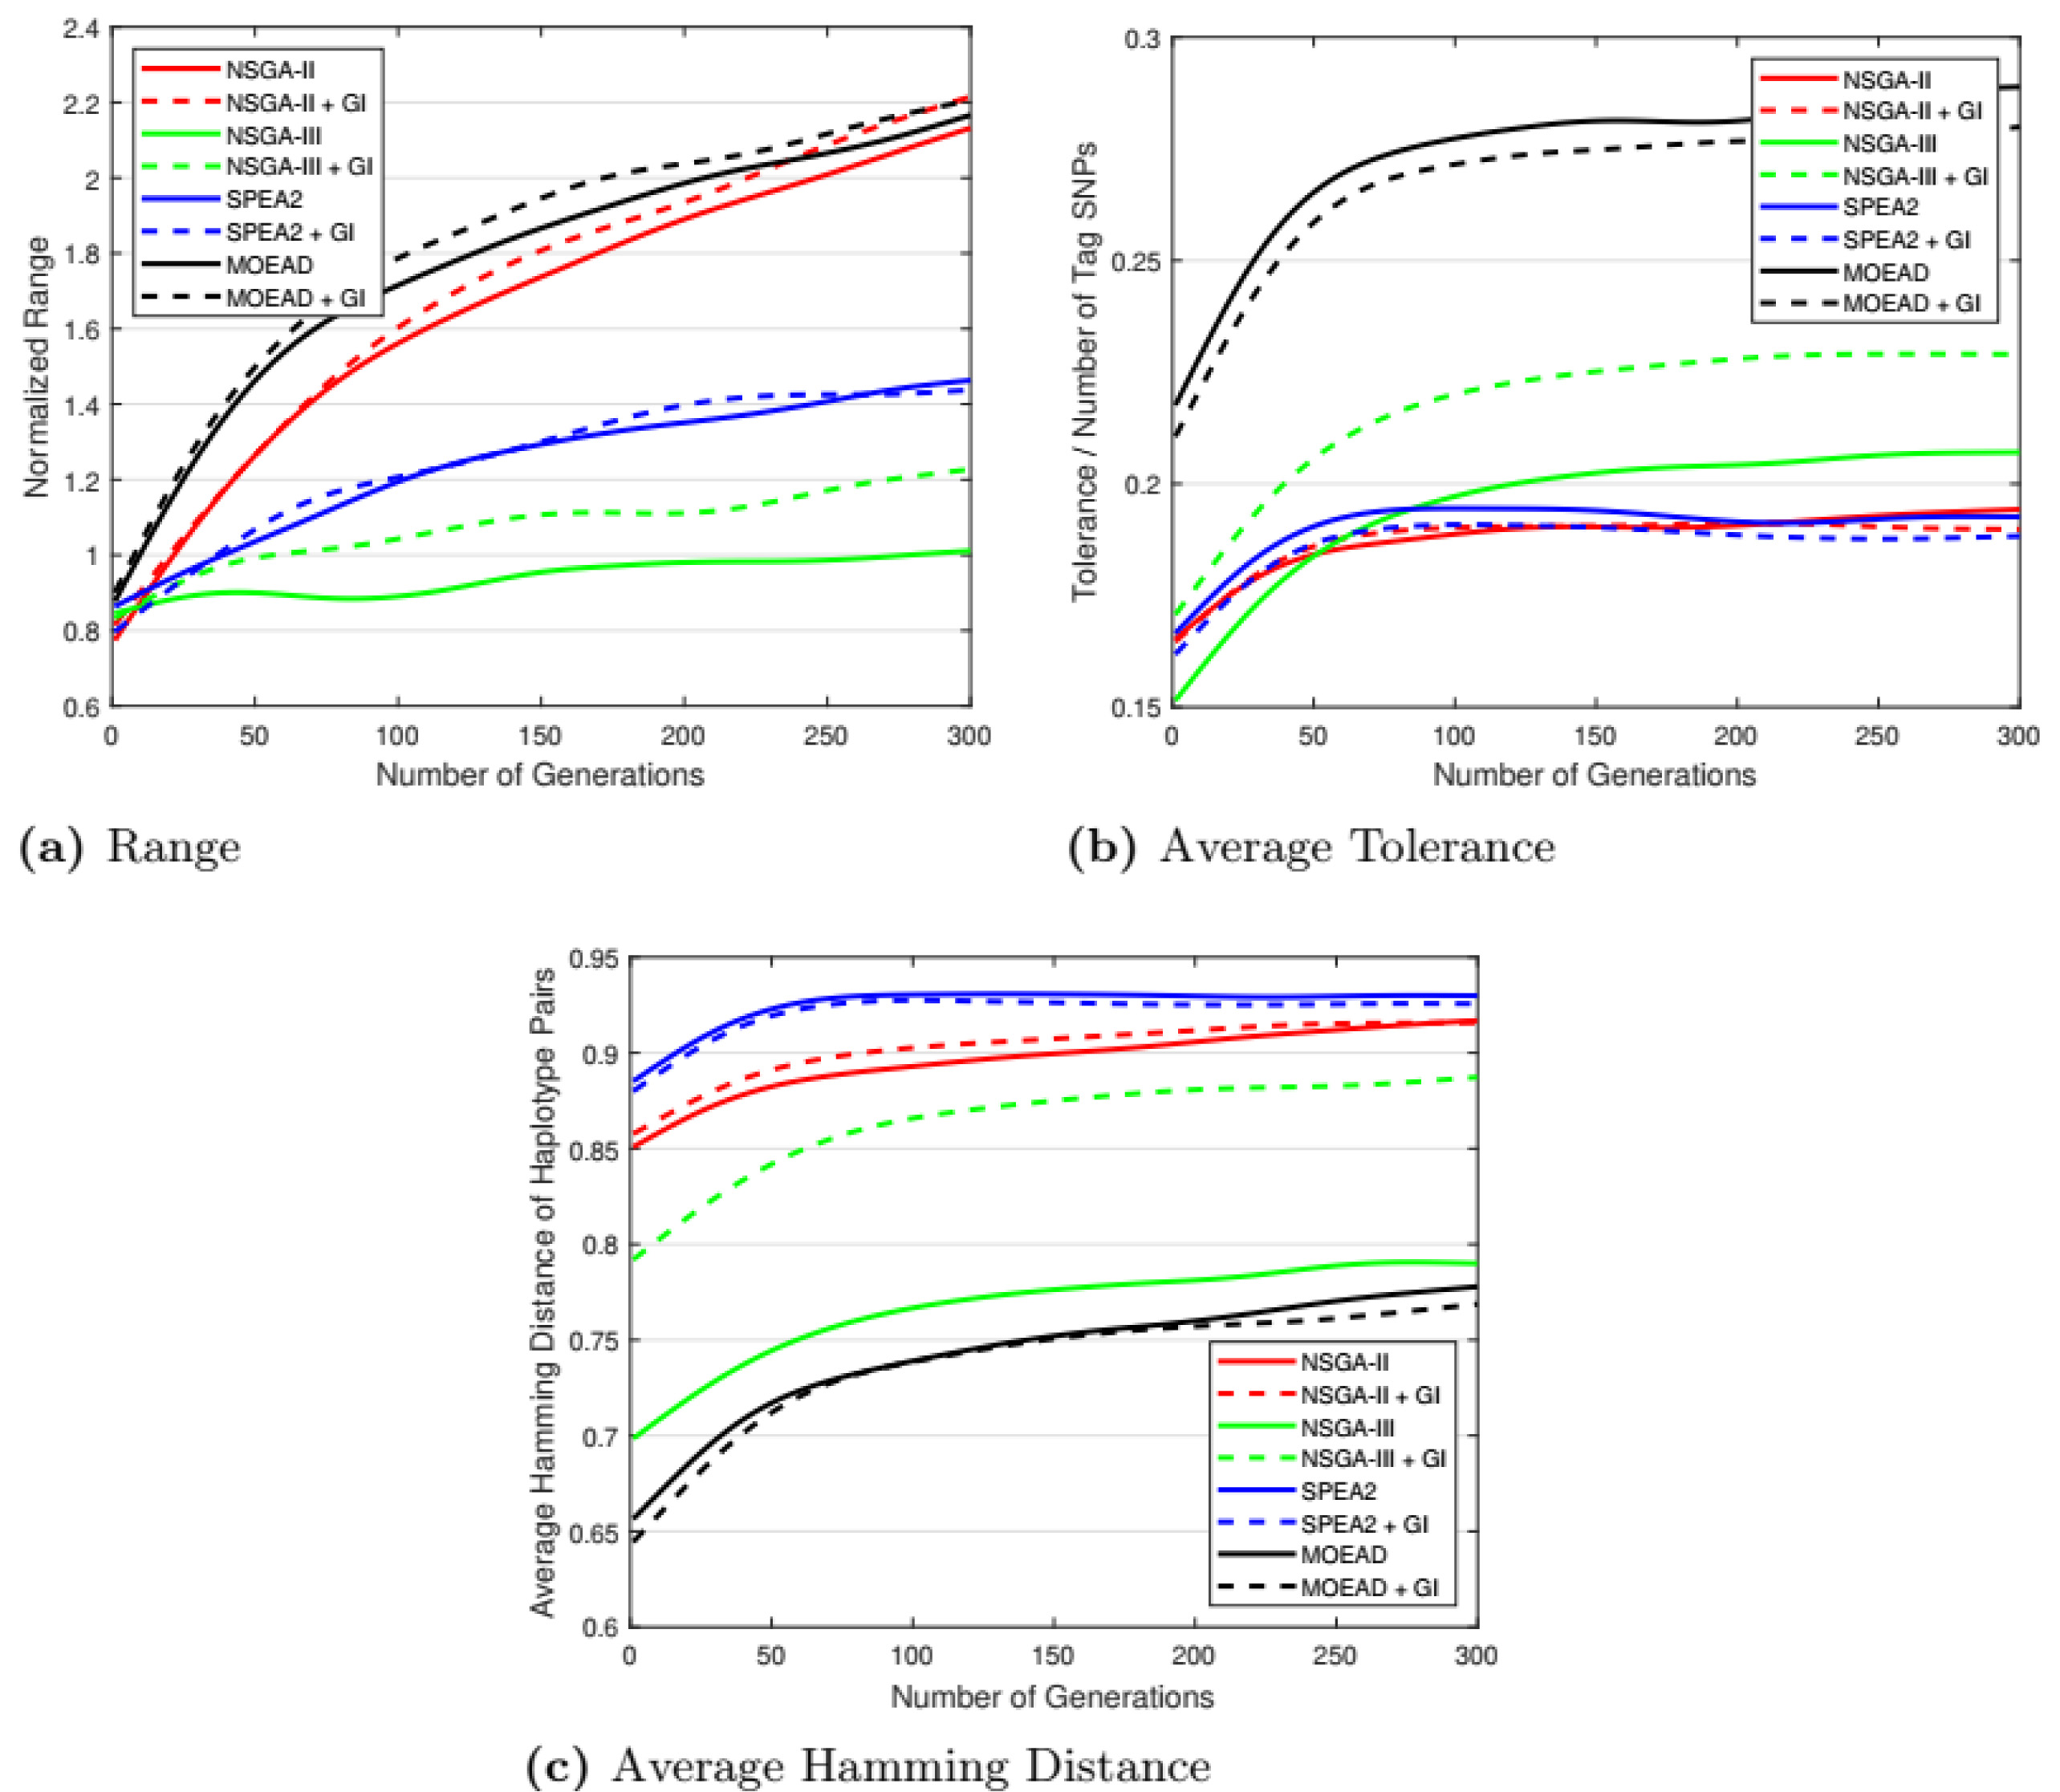
\includegraphics[width=\textwidth]{analisis_assets/moqa_2022/figures/moqa_fig_convergencia_2.jpeg}
        \caption{Estudio de sensibilidad de parámetros genéticos (300 generaciones, población = 100). Análisis focalizado en la robustez de los algoritmos ante una reducción de recursos computacionales.}
    \end{subfigure}
    \caption{Análisis de las trayectorias de convergencia reportadas por Moqa et al. (2022).}
\end{figure}

\subsubsection{Top 10 por métrica (Moqa)}
A continuación se presenta el Top de mejores individuos reportados en el estudio original. Nótese que las métricas de \textit{Hypervolume} y \textit{Range} no fueron facilitadas por los autores.

\begin{table}[H]
    \centering
    \begin{subtable}[t]{0.45\textwidth}
        \centering
        \caption{Range ($\uparrow$)}
        \begin{tabular}{lllc}
            \toprule
            Pos & Algo & Init & Valor \\
            \midrule
            1 & MOEAD & RD & 2.1533 \\
            2 & MOEAD & GH & 2.1382 \\
            3 & NSGA2 & GH & 1.8090 \\
            4 & NSGA2 & RD & 1.7877 \\
            5 & NSGA3 & GH & 1.7563 \\
            6 & SPEA2 & GH & 1.0608 \\
            7 & SPEA2 & RD & 1.0429 \\
            8 & NSGA3 & RD & 0.4639 \\
            \bottomrule
        \end{tabular}
    \end{subtable}
    \hfill
    \begin{subtable}[t]{0.45\textwidth}
        \centering
        \caption{SumMin ($\downarrow$)}
        \begin{tabular}{lllc}
            \toprule
            Pos & Algo & Init & Valor \\
            \midrule
            1 & NSGA3 & RD & 0.1304 \\
            2 & SPEA2 & GH & 0.1768 \\
            3 & NSGA3 & GH & 0.1838 \\
            4 & NSGA2 & GH & 0.2005 \\
            5 & SPEA2 & RD & 0.2135 \\
            6 & NSGA2 & RD & 0.2331 \\
            7 & MOEAD & GH & 0.3018 \\
            8 & MOEAD & RD & 0.4092 \\
            \bottomrule
        \end{tabular}
    \end{subtable}
\end{table}

\begin{table}[H]
    \centering
    \begin{subtable}[t]{0.45\textwidth}
        \centering
        \caption{MinSum ($\downarrow$)}
        \begin{tabular}{lllc}
            \toprule
            Pos & Algo & Init & Valor \\
            \midrule
            1 & NSGA2 & GH & 0.1114 \\
            2 & NSGA3 & RD & 0.1244 \\
            3 & NSGA2 & RD & 0.1310 \\
            4 & SPEA2 & GH & 0.1311 \\
            5 & MOEAD & GH & 0.1578 \\
            6 & SPEA2 & RD & 0.1896 \\
            7 & NSGA3 & GH & 0.1899 \\
            8 & MOEAD & RD & 0.1968 \\
            \bottomrule
        \end{tabular}
    \end{subtable}
    \hfill
    \begin{subtable}[t]{0.45\textwidth}
        \centering
        \caption{Max. Tolerance Rate ($\uparrow$)}
        \begin{tabular}{lllc}
            \toprule
            Pos & Algo & Init & Valor \\
            \midrule
            1 & NSGA3 & GH & 0.0937 \\
            2 & MOEAD & GH & 0.0895 \\
            3 & MOEAD & RD & 0.0891 \\
            4 & NSGA3 & RD & 0.0859 \\
            5 & NSGA2 & GH & 0.0781 \\
            6 & NSGA2 & RD & 0.0692 \\
            7 & SPEA2 & RD & 0.0633 \\
            8 & SPEA2 & GH & 0.0593 \\
            \bottomrule
        \end{tabular}
    \end{subtable}
\end{table}

\begin{table}[H]
    \centering
    \begin{subtable}[t]{0.45\textwidth}
        \centering
        \caption{Avg. Tolerance Rate ($\uparrow$)}
        \begin{tabular}{lllc}
            \toprule
            Pos & Algo & Init & Valor \\
            \midrule
            1 & MOEAD & GH & 0.0879 \\
            2 & MOEAD & RD & 0.0816 \\
            3 & NSGA3 & RD & 0.0726 \\
            4 & NSGA3 & GH & 0.0525 \\
            5 & NSGA2 & GH & 0.0520 \\
            6 & SPEA2 & RD & 0.0487 \\
            7 & NSGA2 & RD & 0.0485 \\
            8 & SPEA2 & GH & 0.0474 \\
            \bottomrule
        \end{tabular}
    \end{subtable}
    \hfill
    \begin{subtable}[t]{0.45\textwidth}
        \centering
        \caption{Avg. Hamming ($\uparrow$)}
        \begin{tabular}{lllc}
            \toprule
            Pos & Algo & Init & Valor \\
            \midrule
            1 & MOEAD & GH & 0.1523 \\
            2 & MOEAD & RD & 0.1500 \\
            3 & NSGA3 & RD & 0.1083 \\
            4 & NSGA2 & GH & 0.1061 \\
            5 & NSGA2 & RD & 0.1022 \\
            6 & NSGA3 & GH & 0.0962 \\
            7 & SPEA2 & RD & 0.0773 \\
            8 & SPEA2 & GH & 0.0769 \\
            \bottomrule
        \end{tabular}
    \end{subtable}
    \caption*{* Los autores no reportaron valores de Hypervolume en su estudio experimental.}
\end{table}

\subsubsection{Ranking Global}
El análisis del ranking global mediante el método \textit{Rank-Sum} (suma de posiciones en las 6 métricas reportadas) permite identificar las configuraciones más equilibradas del estudio original.

\begin{table}[H]
    \centering
    \begin{tabular}{lllc}
        \toprule
        Pos & Algo & Init & Score (Rank-Sum) \\
        \midrule
        1 & MOEAD & GH & 18.0 \\
        2 & NSGA3 & RD & 21.0 \\
        3 & NSGA2 & GH & 22.0 \\
        4 & MOEAD & RD & 24.0 \\
        5 & NSGA3 & GH & 26.0 \\
        6 & NSGA2 & RD & 31.0 \\
        7 & SPEA2 & GH & 36.0 \\
        8 & SPEA2 & RD & 38.0 \\
        \bottomrule
    \end{tabular}
    \caption{Ranking Global (Rank-Sum) para el reporte de Moqa et al. (2022). El cálculo se basa exclusivamente en las posiciones obtenidas en las 6 métricas detalladas anteriormente (Range, SumMin, MinSum, Max. Tolerance Rate, Avg. Tolerance Rate y Avg. Hamming).}
\end{table}


\subsubsection{Conclusiones y comparación con las conclusiones del documento}

\paragraph{Análisis de los resultados obtenidos}
\begin{itemize}
    \item \textbf{Superioridad de MOEA/D:} La variante MOEA/D con inicialización heurística (GH) demuestra ser la configuración más equilibrada globalmente, liderando las métricas de tolerancia media y diversidad genética (Hamming).
    \item \textbf{Rendimiento de NSGA-III:} Resulta notable la capacidad de NSGA-III para obtener la segunda posición global utilizando únicamente inicialización aleatoria (RD), destacando especialmente en la convergencia del peor caso (SumMin).
    \item \textbf{Rezagos de SPEA2:} Independientemente de la estrategia de inicialización, SPEA2 muestra el desempeño más débil del conjunto, ocupando las últimas posiciones en tolerancia y diversidad.
\end{itemize}

\paragraph{Comparación empírica con Moqa et al. (2022)}
\begin{itemize}
    \item \textbf{Jerarquía algorítmica y Many-Objective Optimization:} El estudio original fundamenta la superioridad de los algoritmos de \textit{many-objective optimization} (MOEA/D y NSGA-III) frente a modelos multiobjetivo clásicos como NSGA-II y SPEA2, argumentando que estos últimos presentan limitaciones al escalar en el número de objetivos. Nuestros resultados validan parcialmente esta premisa, situando a MOEA/D en el primer puesto del ranking global (\textit{Rank-Sum}), aunque revelan una competitividad notable de NSGA-II bajo configuraciones heurísticas específicas.
    \item \textbf{Impacto de la inicialización heurística (Greedy vs. Random):} Se confirma la tesis de los autores sobre la ventaja competitiva de la inicialización \textit{greedy}. Según el reporte original, este método no solo mejora la calidad de las soluciones iniciales sino que facilita la obtención de un conjunto más amplio de soluciones no dominadas, proporcionando mayor flexibilidad para adaptarse a diferentes plataformas de genotipado y necesidades del usuario final.
    \item \textbf{Limitaciones en la evaluación de robustez:} Aunque Moqa et al. declaran a MOEA/D como el algoritmo dominante en «la mayoría de los casos», nuestro desglose analítico mediante el método \textit{Rank-Sum} revela que la ausencia de métricas integradoras como el \textit{Hypervolume} en su reporte original oculta matices críticos sobre la estabilidad y el compromiso real entre convergencia y diversidad que solo una evaluación agregada permite desvelar.
\end{itemize}


% =========================================================
\section{Mis experimentos}
\label{sec:mis_experimentos}

% =========================================================
\subsection{Reporte 2 — Ejecución A: 20260420T205406}
\label{sec:reporte2}

\subsubsection{Configuración}

\paragraph{Configuración resumida}
\begin{itemize}
    \item \textbf{Infraestructura:} Implementada mediante la librería especializada \textbf{pymoo} (Python).
    \item \textbf{Dataset:} Benchmark biológico Hinds 2005. Se utilizan 772 marcadores genéticos (SNPs) polimórficos tras filtrar los 1032 originales, con una estructura de 48 patrones alélicos.
    \item \textbf{Configuración Global:}
    \begin{itemize}
        \item \textbf{Transformación de objetivos:} Negación lineal ($f' = -f$) para convertir la maximización en minimización sin distorsionar el espacio biológico.
        \item \textbf{Normalización:} Escalado estático basado en los límites del conjunto de datos \\ (modo \textbf{\texttt{static\_dataset\_limits}}). Se explica en detalle en la siguiente sección.
    \end{itemize}
    \item \textbf{Parámetros de los Algoritmos:}
    \begin{itemize}
        \item \textbf{Ajustes generales:}
        \begin{itemize}
            \item \textbf{Tamaño de la población:} 200 individuos.
            \item \textbf{Número de generaciones:} 500.
            \item \textbf{Número de descendientes por generación:} 200.
            \item \textbf{Número de ejecuciones independientes:} 5 (para validación estadística).
            \item \textbf{Probabilidad de cruce:} 70\% (Cruce Uniforme).
            \item \textbf{Probabilidad de mutación:} Definida matemáticamente como la inversa de la longitud del cromosoma ($1/L \approx 0,0013$), lo que equivale estadísticamente a la alteración de un único gen por individuo.
        \end{itemize}
        \item \textbf{Ajustes específicos de los algoritmos:}
        \begin{itemize}
            \item \textbf{NSGA-II / SPEA2:} Basados en ordenamiento por dominancia y densidad de soluciones.
            \item \textbf{NSGA-III:} 8 particiones por objetivo para generar un conjunto de 165 direcciones de referencia.
            \item \textbf{MOEA/D (TCHE, PBI, WS):}
            \begin{itemize}
                \item \textbf{Tamaño del vecindario:} 15 subproblemas.
                \item \textbf{Probabilidad de selección en vecindad:} 90\%.
                \item \textbf{Valor de penalización PBI:} 5.0.
            \end{itemize}
        \end{itemize}
    \end{itemize}
    \item \textbf{Estrategias de Inicialización:}
    \begin{itemize}
        \item \texttt{random\_sparse}: \textbf{Aleatoria Dispersa}. Inicialización con baja densidad de selección (9\% de SNPs activos). Está orientada a descubrir paneles de SNPs muy reducidos y eficientes desde el inicio de la búsqueda.
        \item \texttt{random\_dense}: \textbf{Aleatoria Densa}. Inicialización con alta densidad de selección (50\% de SNPs activos). Su objetivo es evaluar el potencial del algoritmo para simplificar y podar conjuntos de datos con gran cantidad de información redundante.
        \item \texttt{greedy\_pure}: \textbf{Voraz Pura}. Técnica de construcción incremental que asegura la cobertura total de los pares de haplotipos. Garantiza que todos los individuos de la población inicial representen soluciones biológicamente válidas (factibles).
        \item \texttt{greedy\_hybrid}: \textbf{Híbrida Voraz}. Enfoque combinado que alterna entre la lógica voraz y el muestreo aleatorio (proporción 50/50). Persigue un equilibrio óptimo entre la calidad inicial de las soluciones y la diversidad genética necesaria para evitar el estancamiento.
    \end{itemize}
    \item \textbf{Tiempo de ejecución de experimentos:} 1 hora y 3 minutos para completar el total de 120 ejecuciones individuales.
\end{itemize}

\paragraph{Profundización de la configuración}
\subparagraph{Normalización}
El sistema emplea el modo \textbf{\texttt{static\_dataset\_limits}}:
\begin{equation}
\label{eq:norm_A}
F_{norm} = \frac{f - f_{ideal}}{f_{nadir} - f_{ideal}}
\end{equation}

\subsubsection*{Ejemplo de cálculo para Diversidad (Hamming)}
Si $f_{ideal} = -250$, $f_{nadir} = 0$ y se alcanza un Hamming de $150$:
\begin{equation}
F_{norm} = \frac{-150 - (-250)}{0 - (-250)} = \frac{100}{250} = \mathbf{0.40}
\end{equation}
*Interpretación:* El valor 0.40 indica que la solución ha capturado el 60\% del potencial de diversidad total del dataset.

\subsubsection{Resultados y análisis (A)}

\paragraph{Frente de Pareto Global}
\begin{figure}[H]
    \centering
    
\includegraphics[width=0.6\textwidth]{analisis_assets/20260420T205406/2_comparativa/1_frentes/frentes_pareto/frentes_pareto_global_full.png}
    \caption{Frente de Pareto Global consolidado para la Ejecución A.}
\end{figure}

\paragraph{Frentes de Pareto (Convergencia final)}

\begin{table}[H]
    \centering
    \begin{tabular}{m{2.2cm} >{\centering\arraybackslash}m{3.2cm} >{\centering\arraybackslash}m{3.2cm} >{\centering\arraybackslash}m{3.2cm} >{\centering\arraybackslash}m{3.2cm}}
        \toprule
        Algoritmo & random\_sparse & random\_dense & greedy\_pure & greedy\_hybrid \\
        \midrule
        \textbf{NSGA-II} & 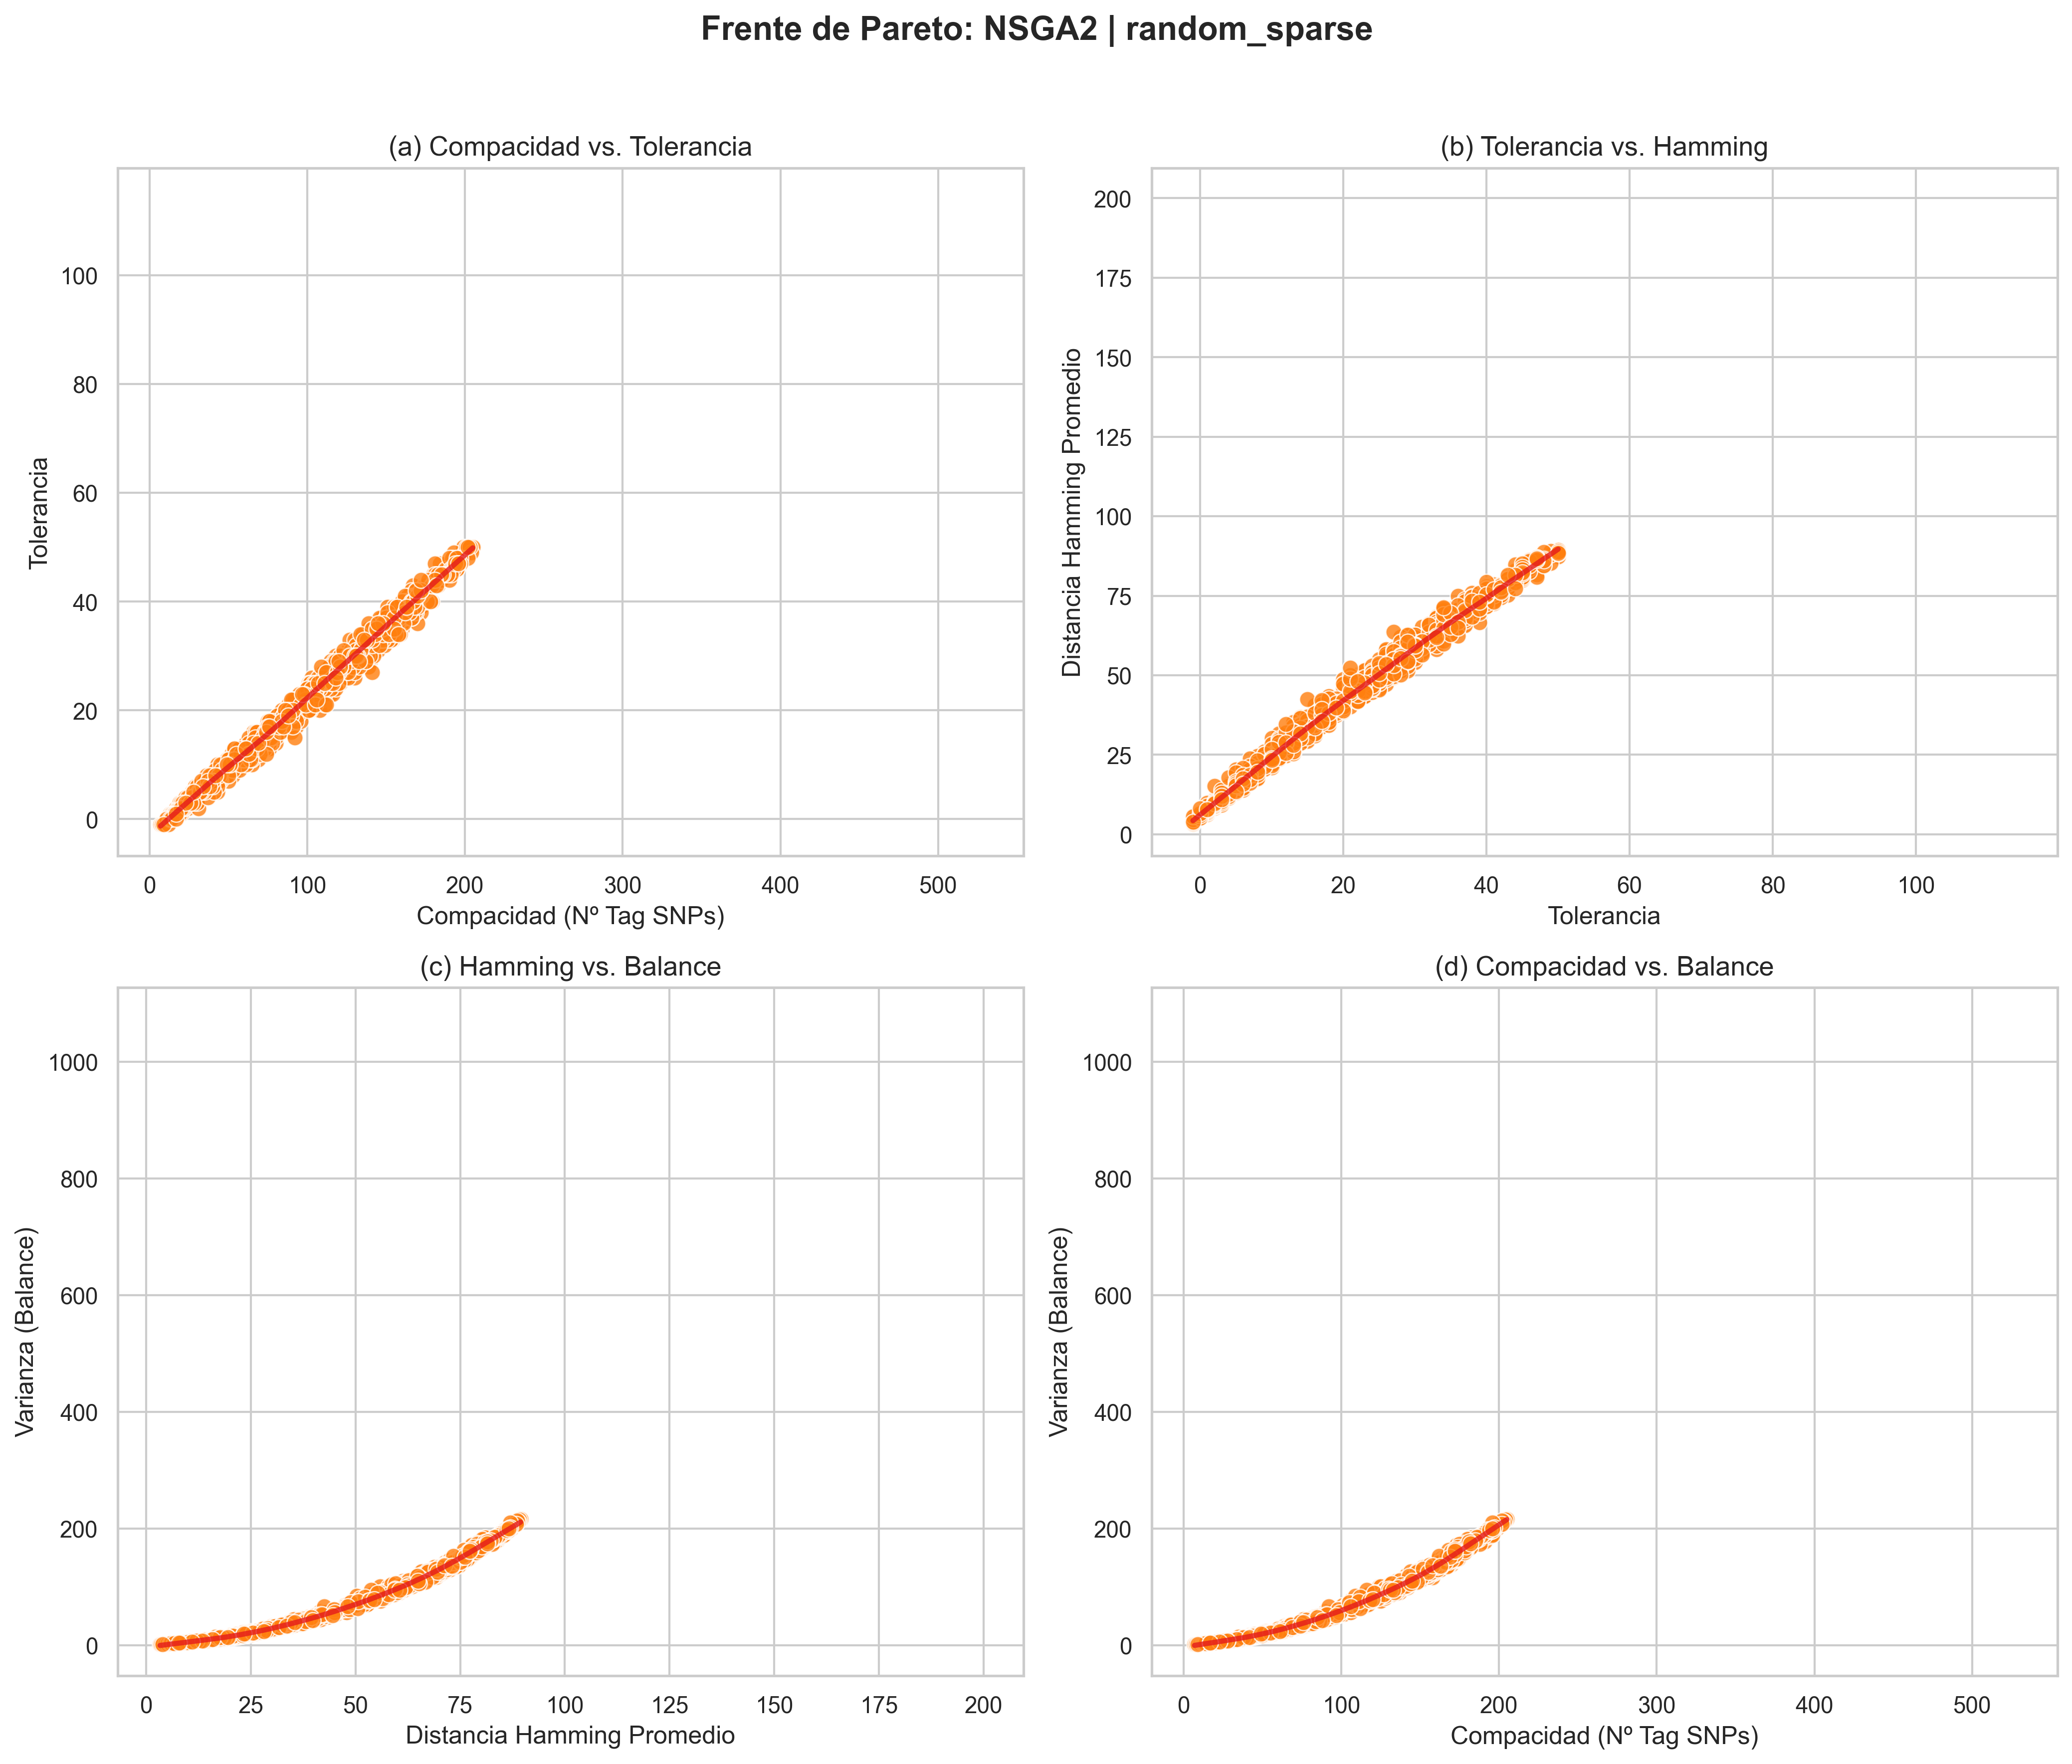
\includegraphics[width=\linewidth]{analisis_assets/20260420T205406/2_comparativa/1_frentes/frentes_pareto/frentes_pareto_nsga2_random_sparse_full.png} & 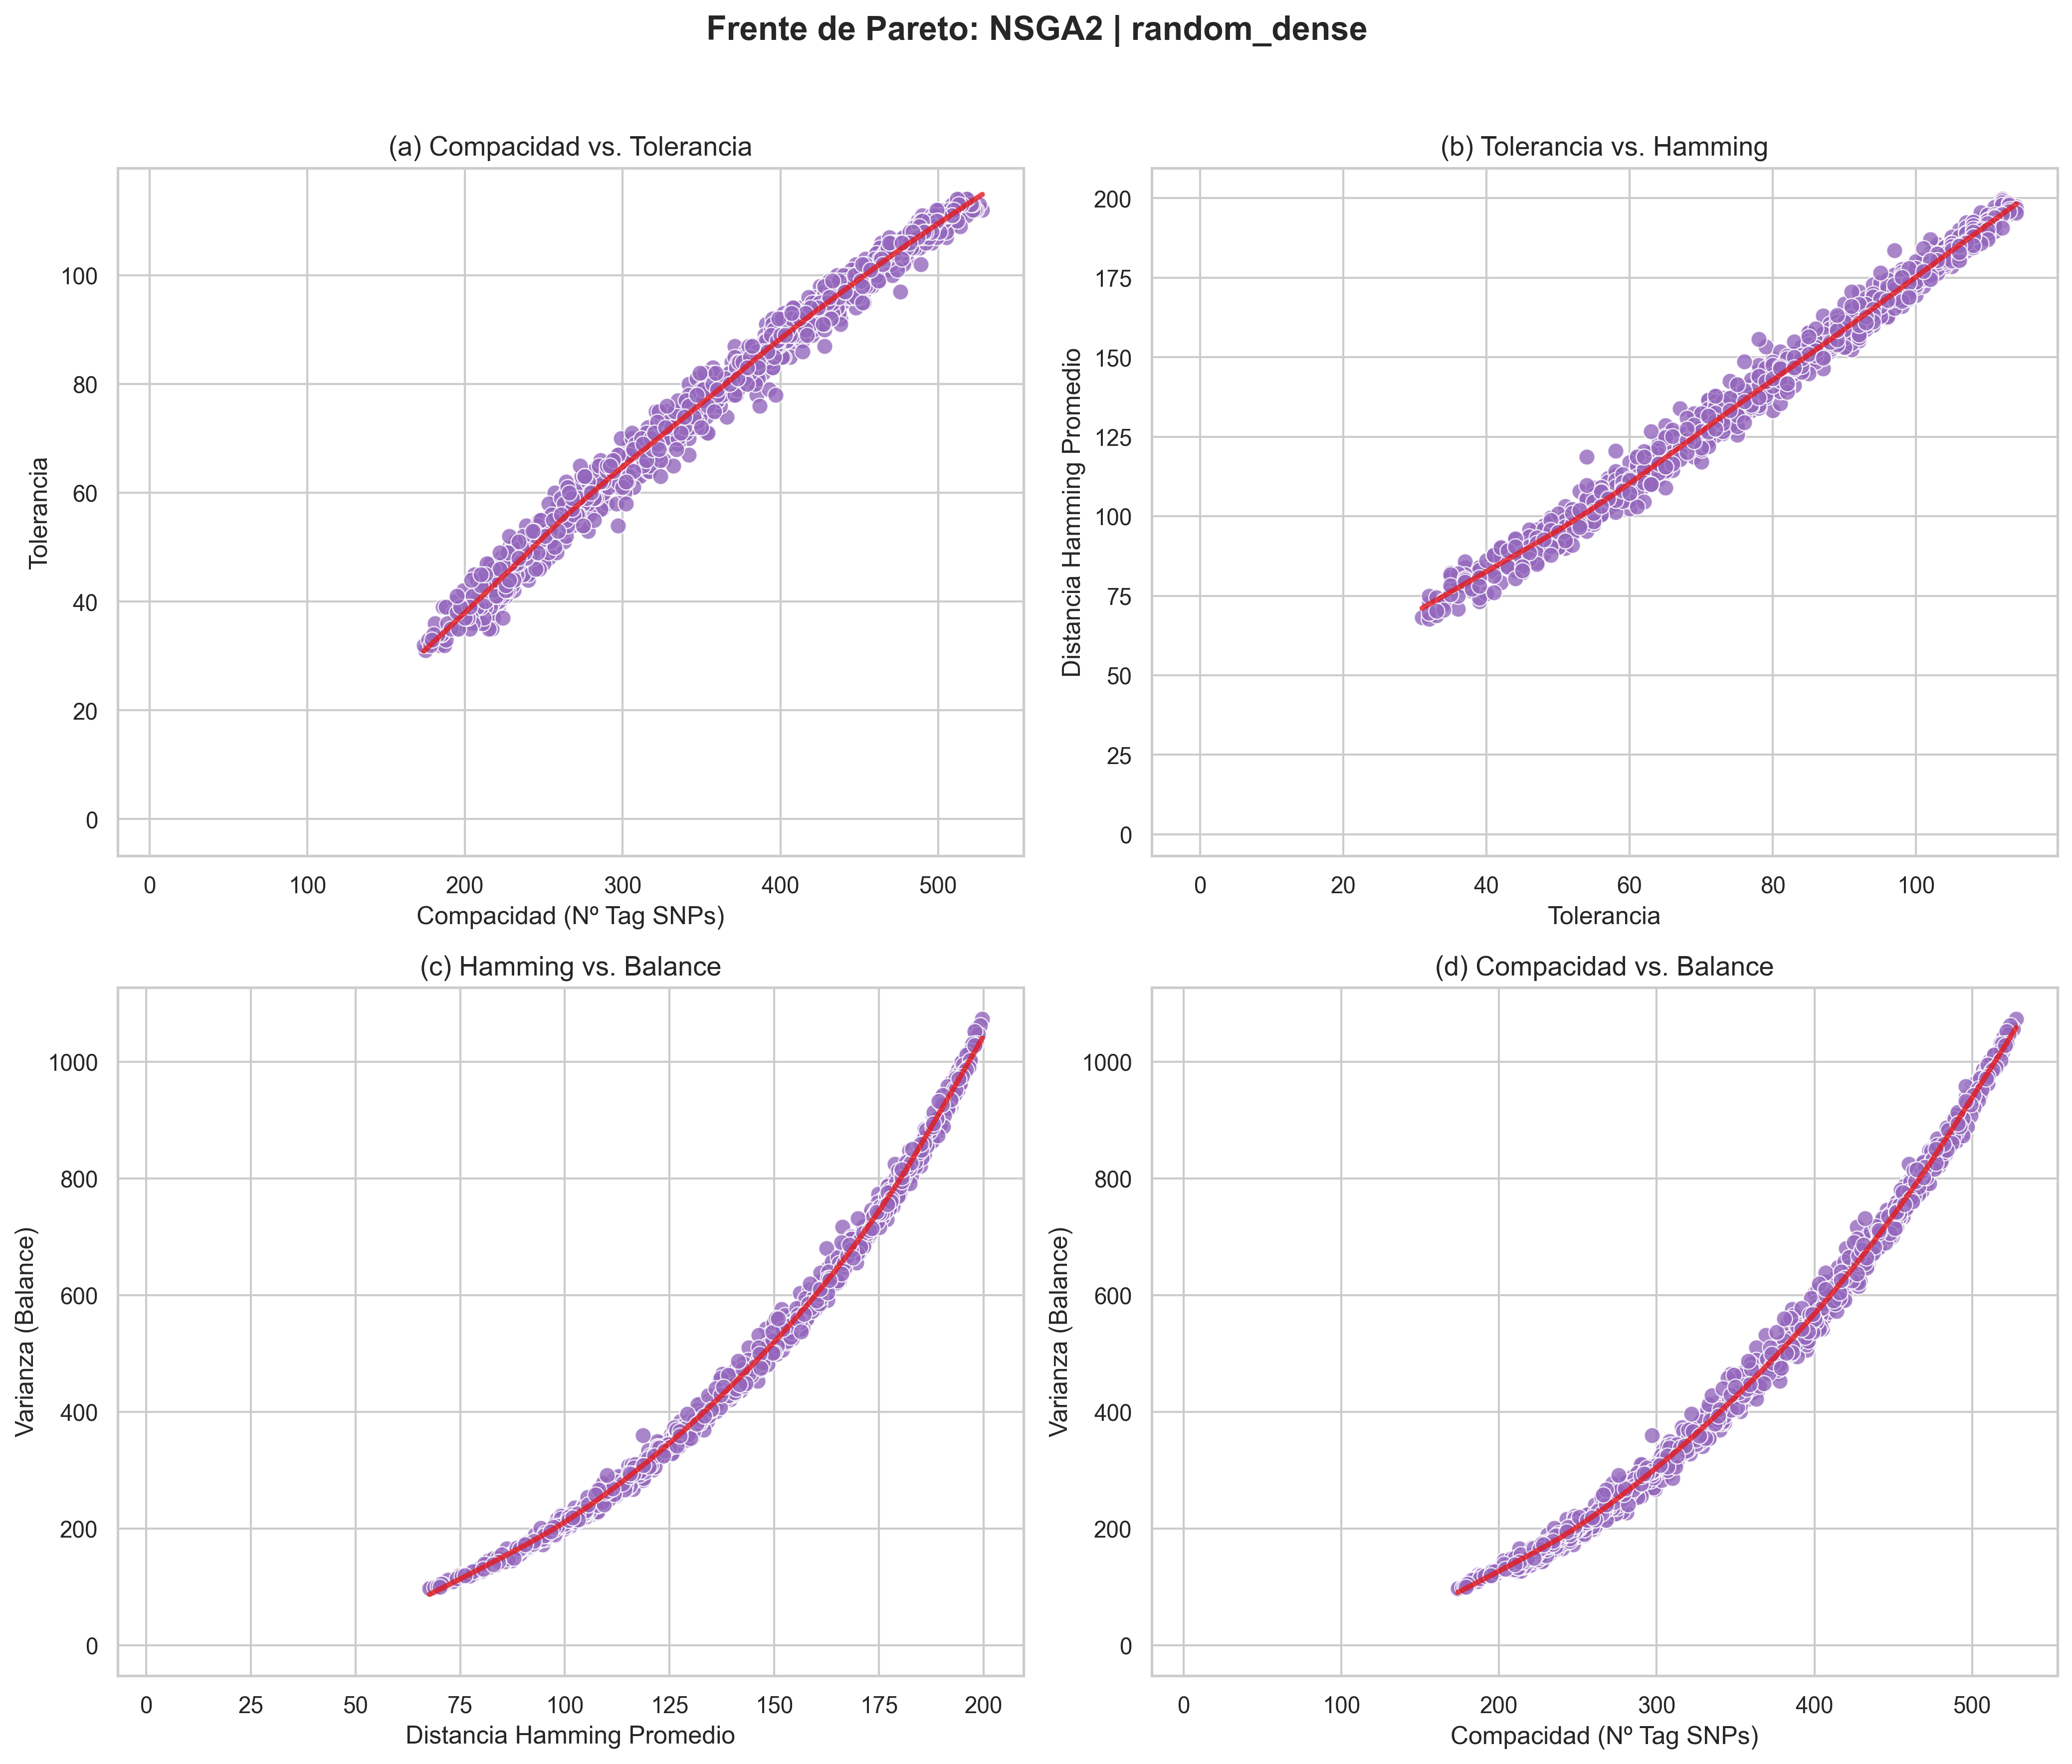
\includegraphics[width=\linewidth]{analisis_assets/20260420T205406/2_comparativa/1_frentes/frentes_pareto/frentes_pareto_nsga2_random_dense_full.png} & 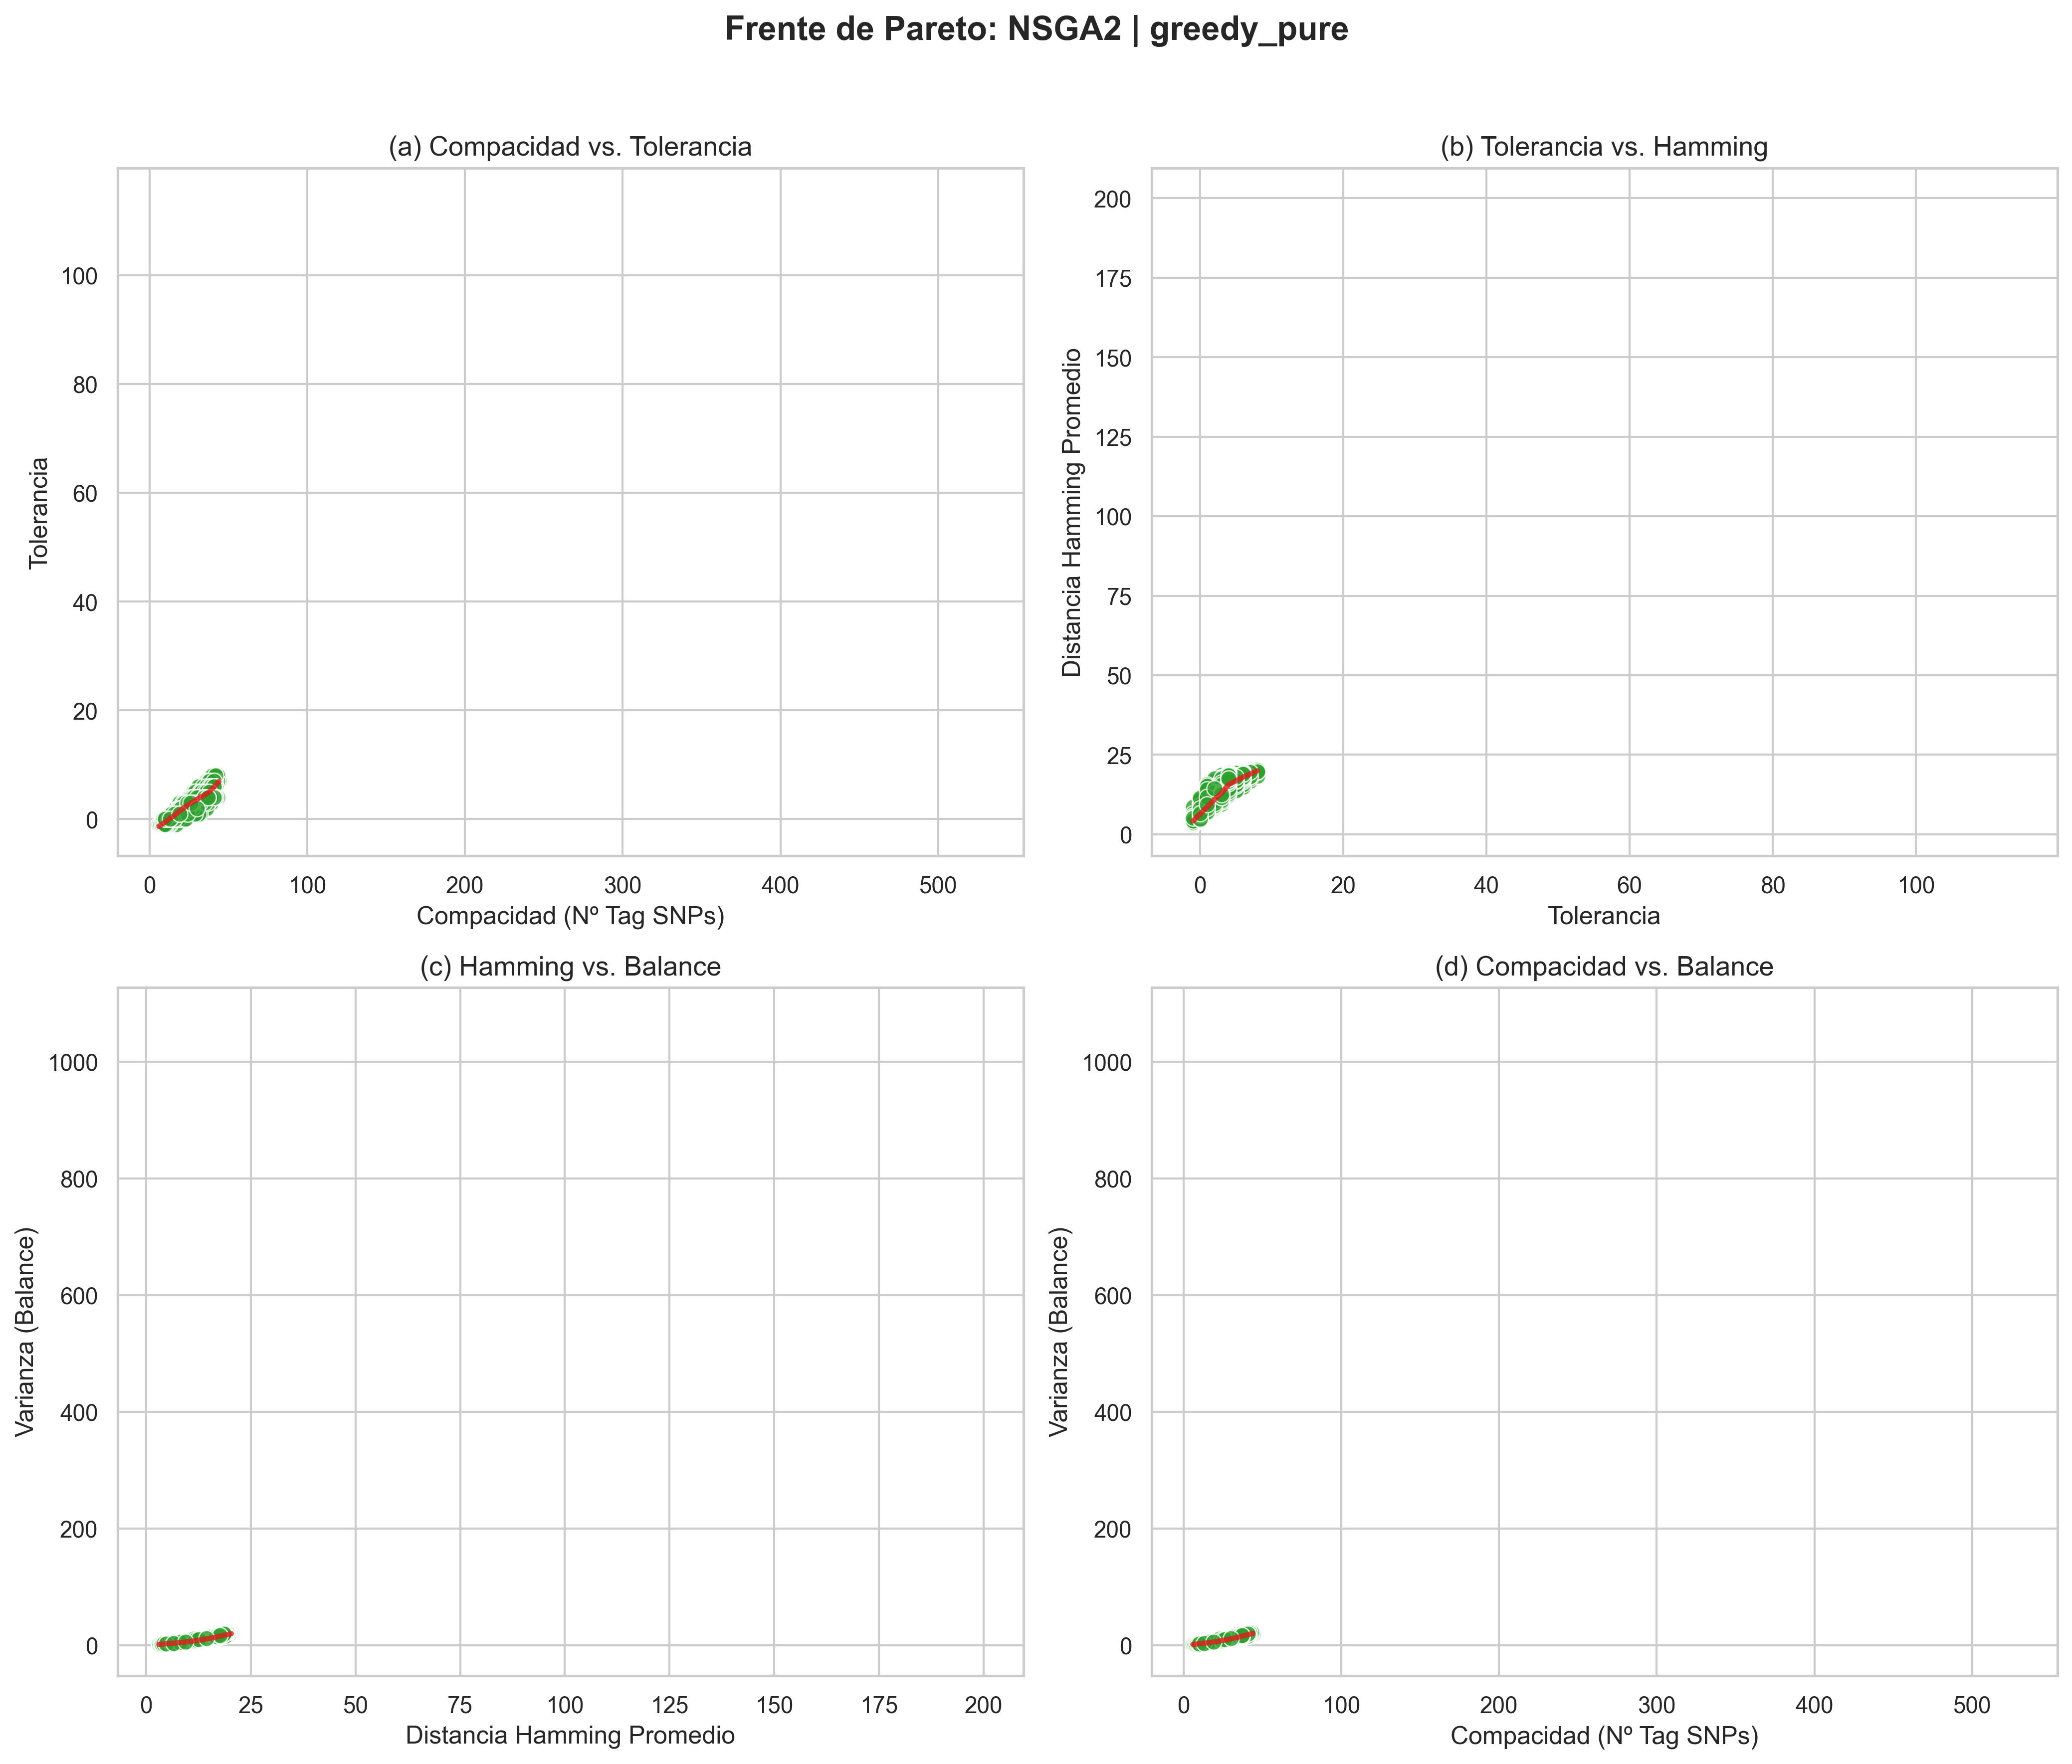
\includegraphics[width=\linewidth]{analisis_assets/20260420T205406/2_comparativa/1_frentes/frentes_pareto/frentes_pareto_nsga2_greedy_pure_full.png} & 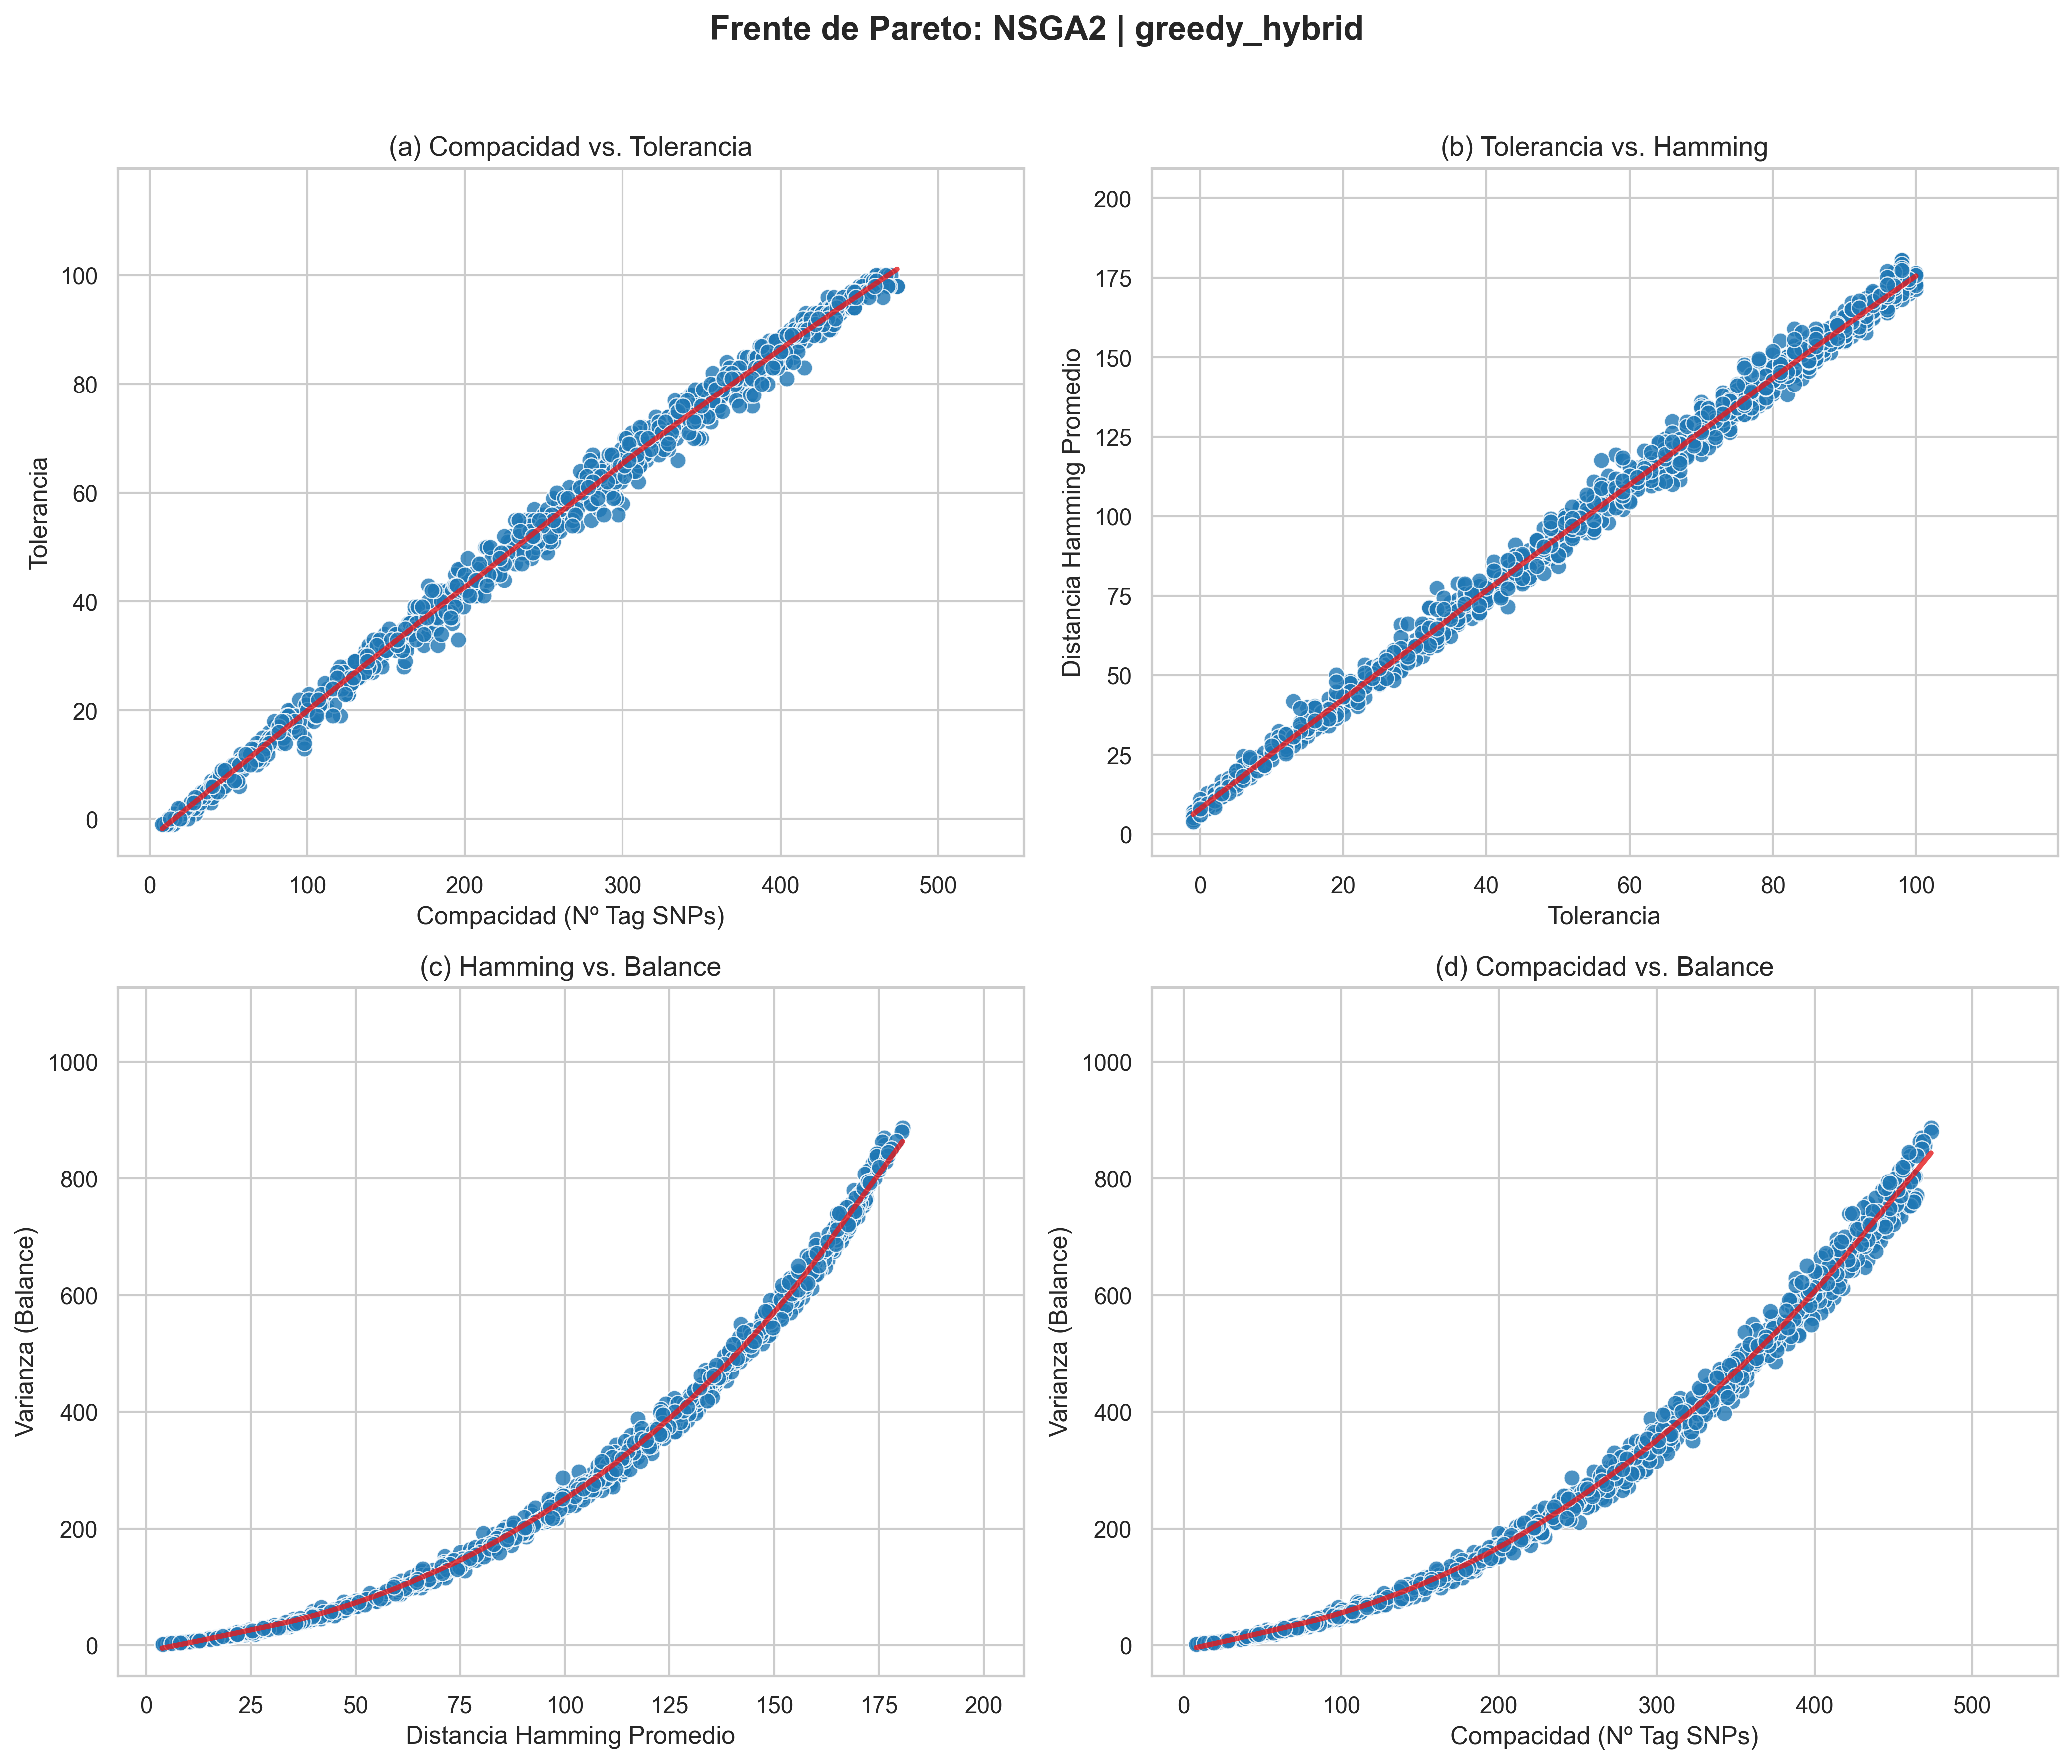
\includegraphics[width=\linewidth]{analisis_assets/20260420T205406/2_comparativa/1_frentes/frentes_pareto/frentes_pareto_nsga2_greedy_hybrid_full.png} \\
        \textbf{NSGA-III} & 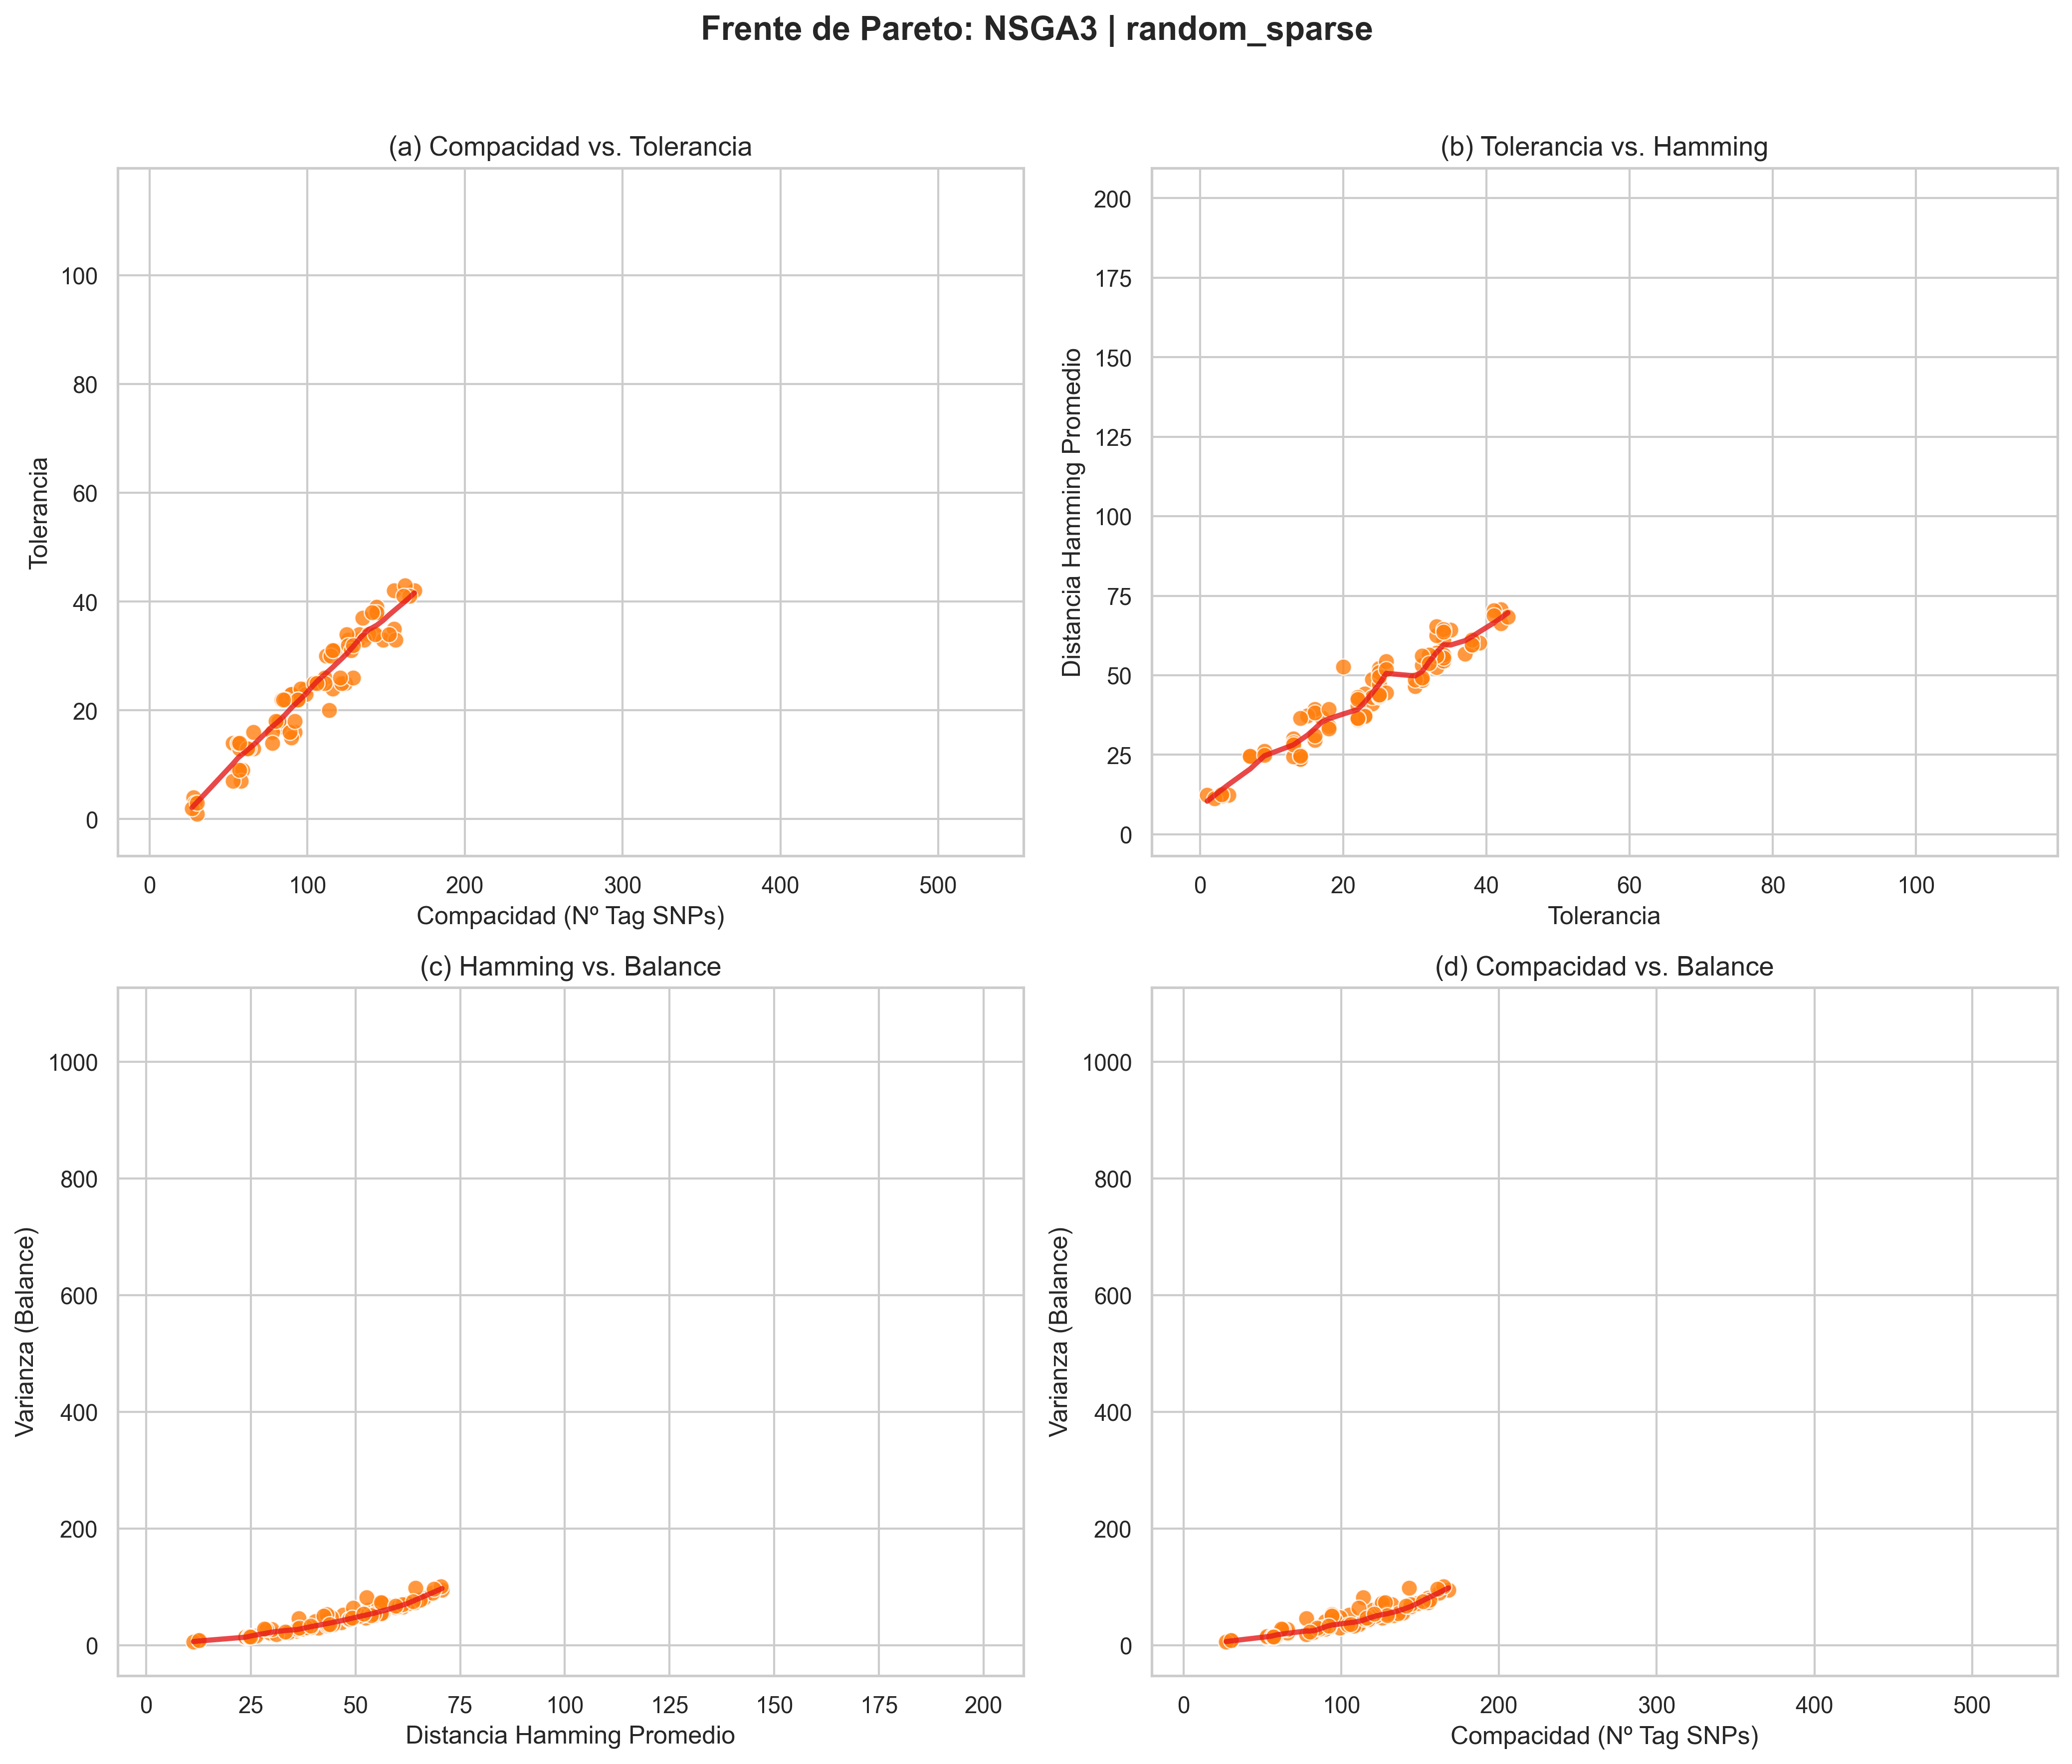
\includegraphics[width=\linewidth]{analisis_assets/20260420T205406/2_comparativa/1_frentes/frentes_pareto/frentes_pareto_nsga3_random_sparse_full.png} & 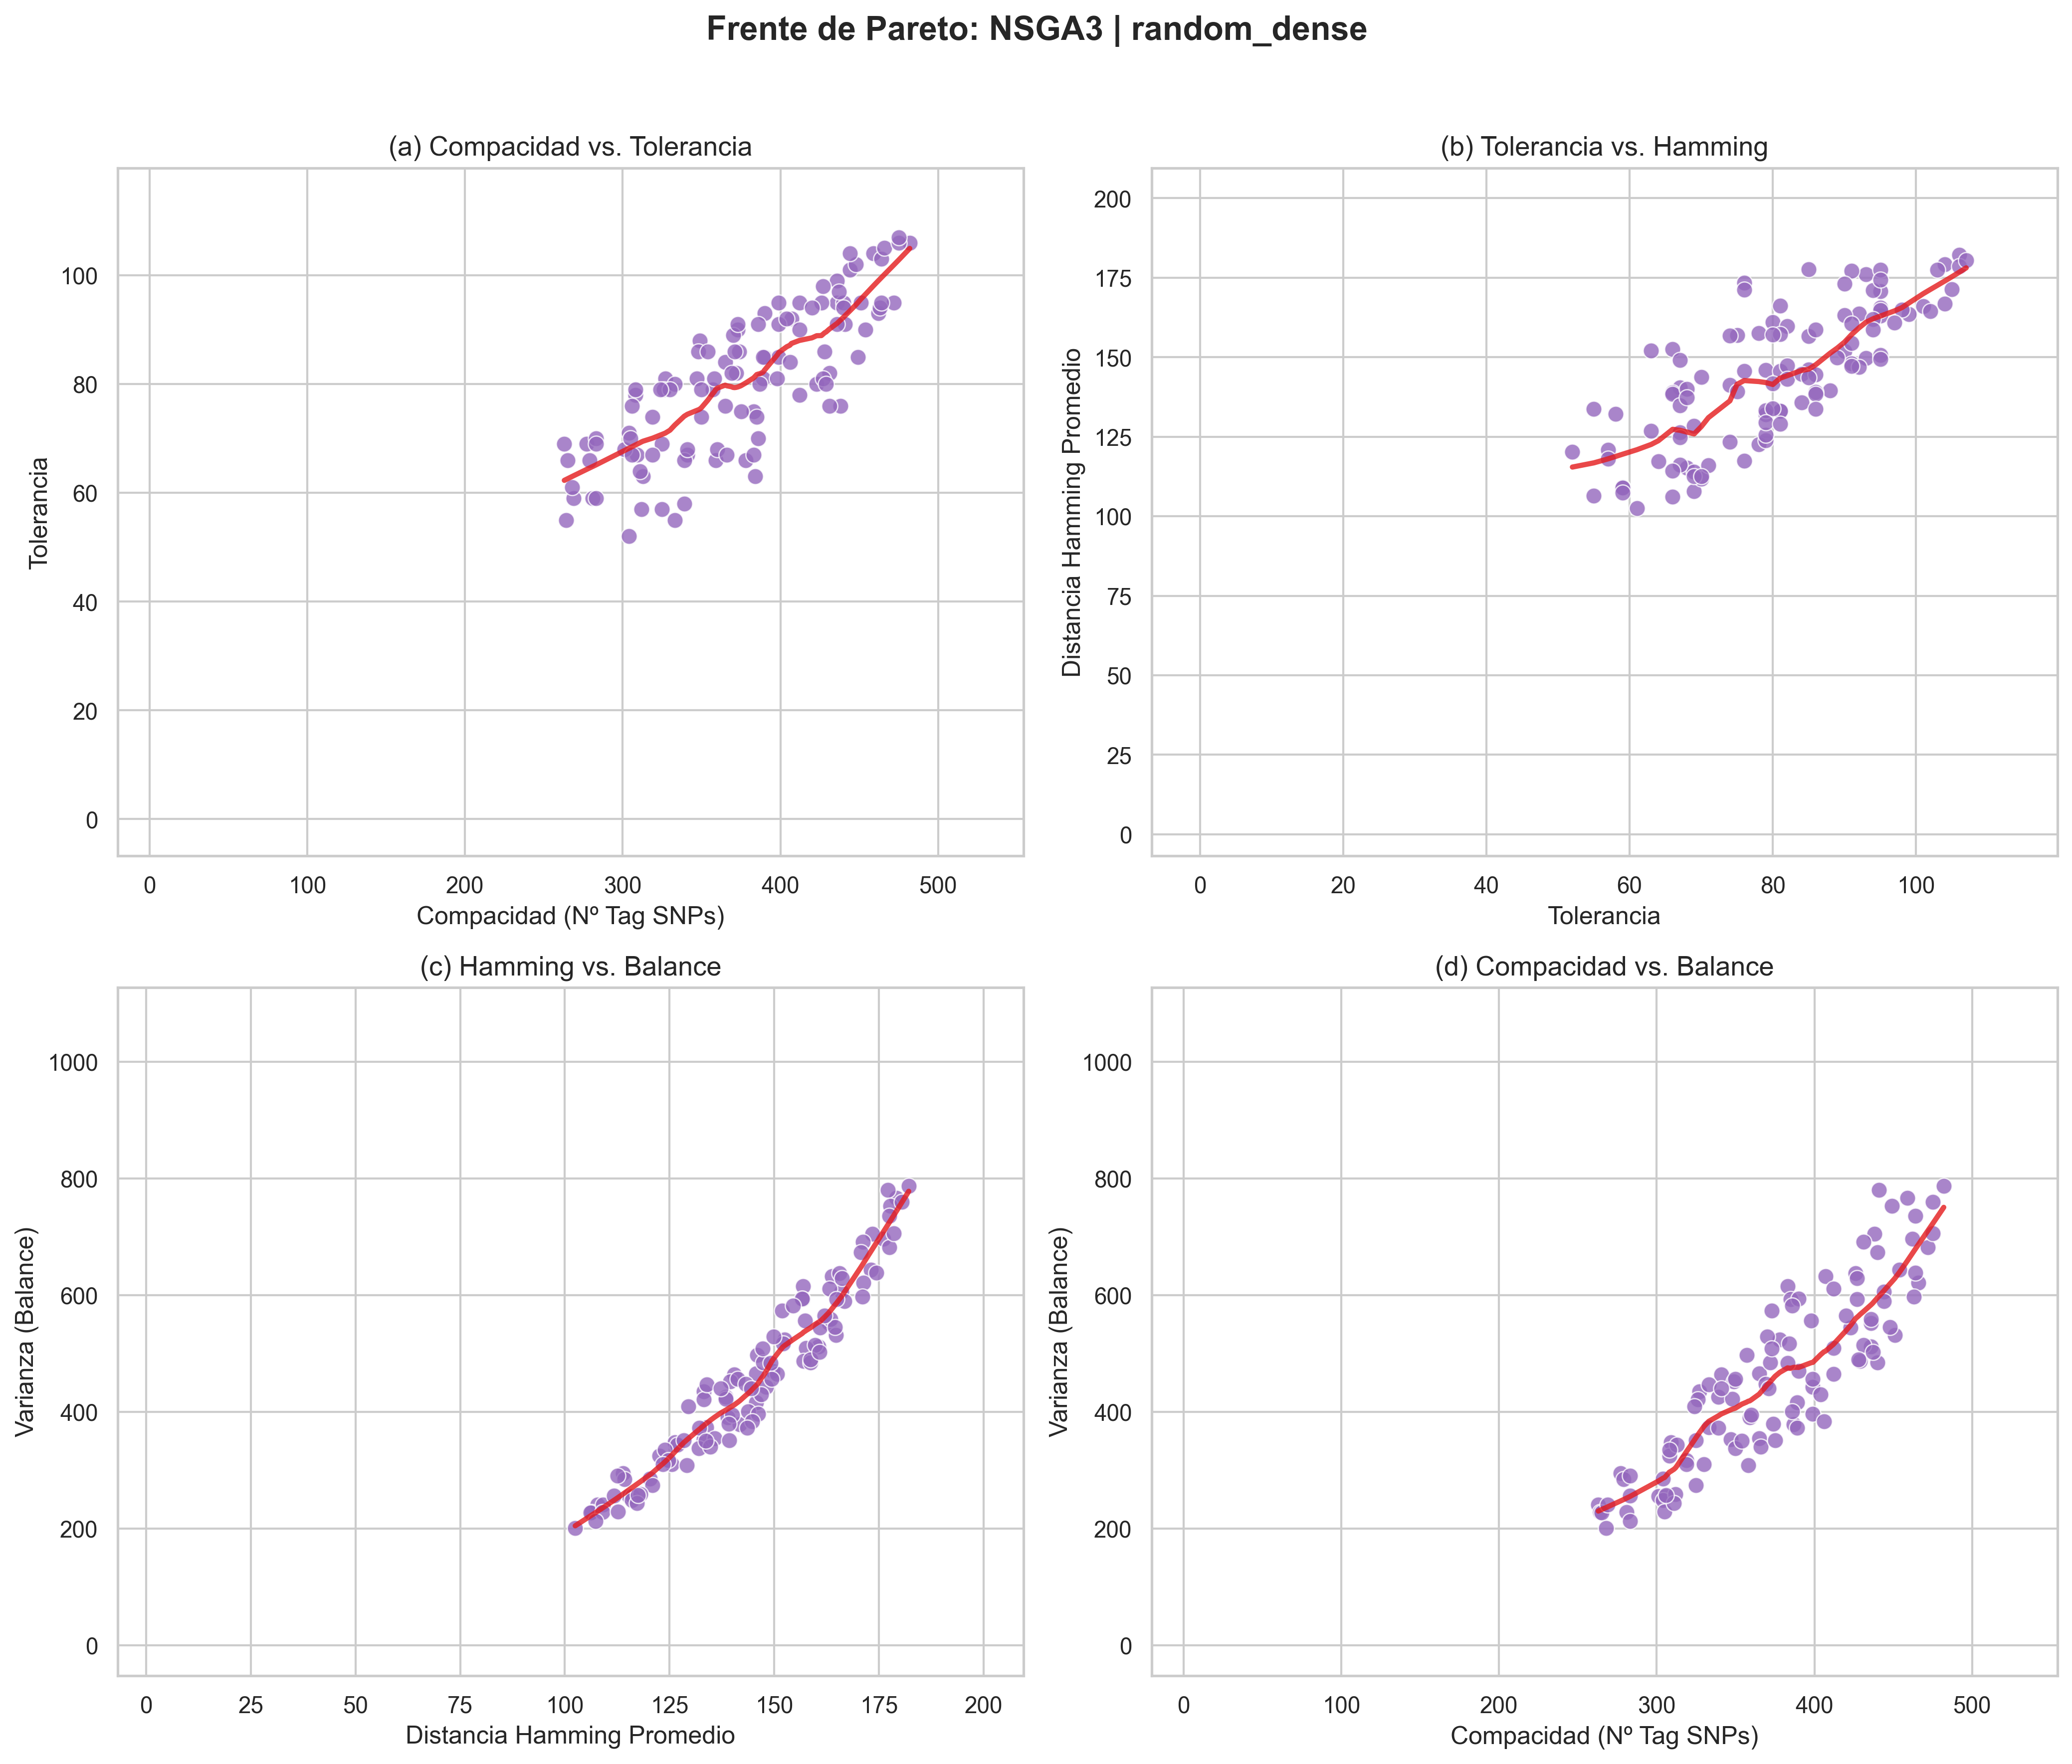
\includegraphics[width=\linewidth]{analisis_assets/20260420T205406/2_comparativa/1_frentes/frentes_pareto/frentes_pareto_nsga3_random_dense_full.png} & 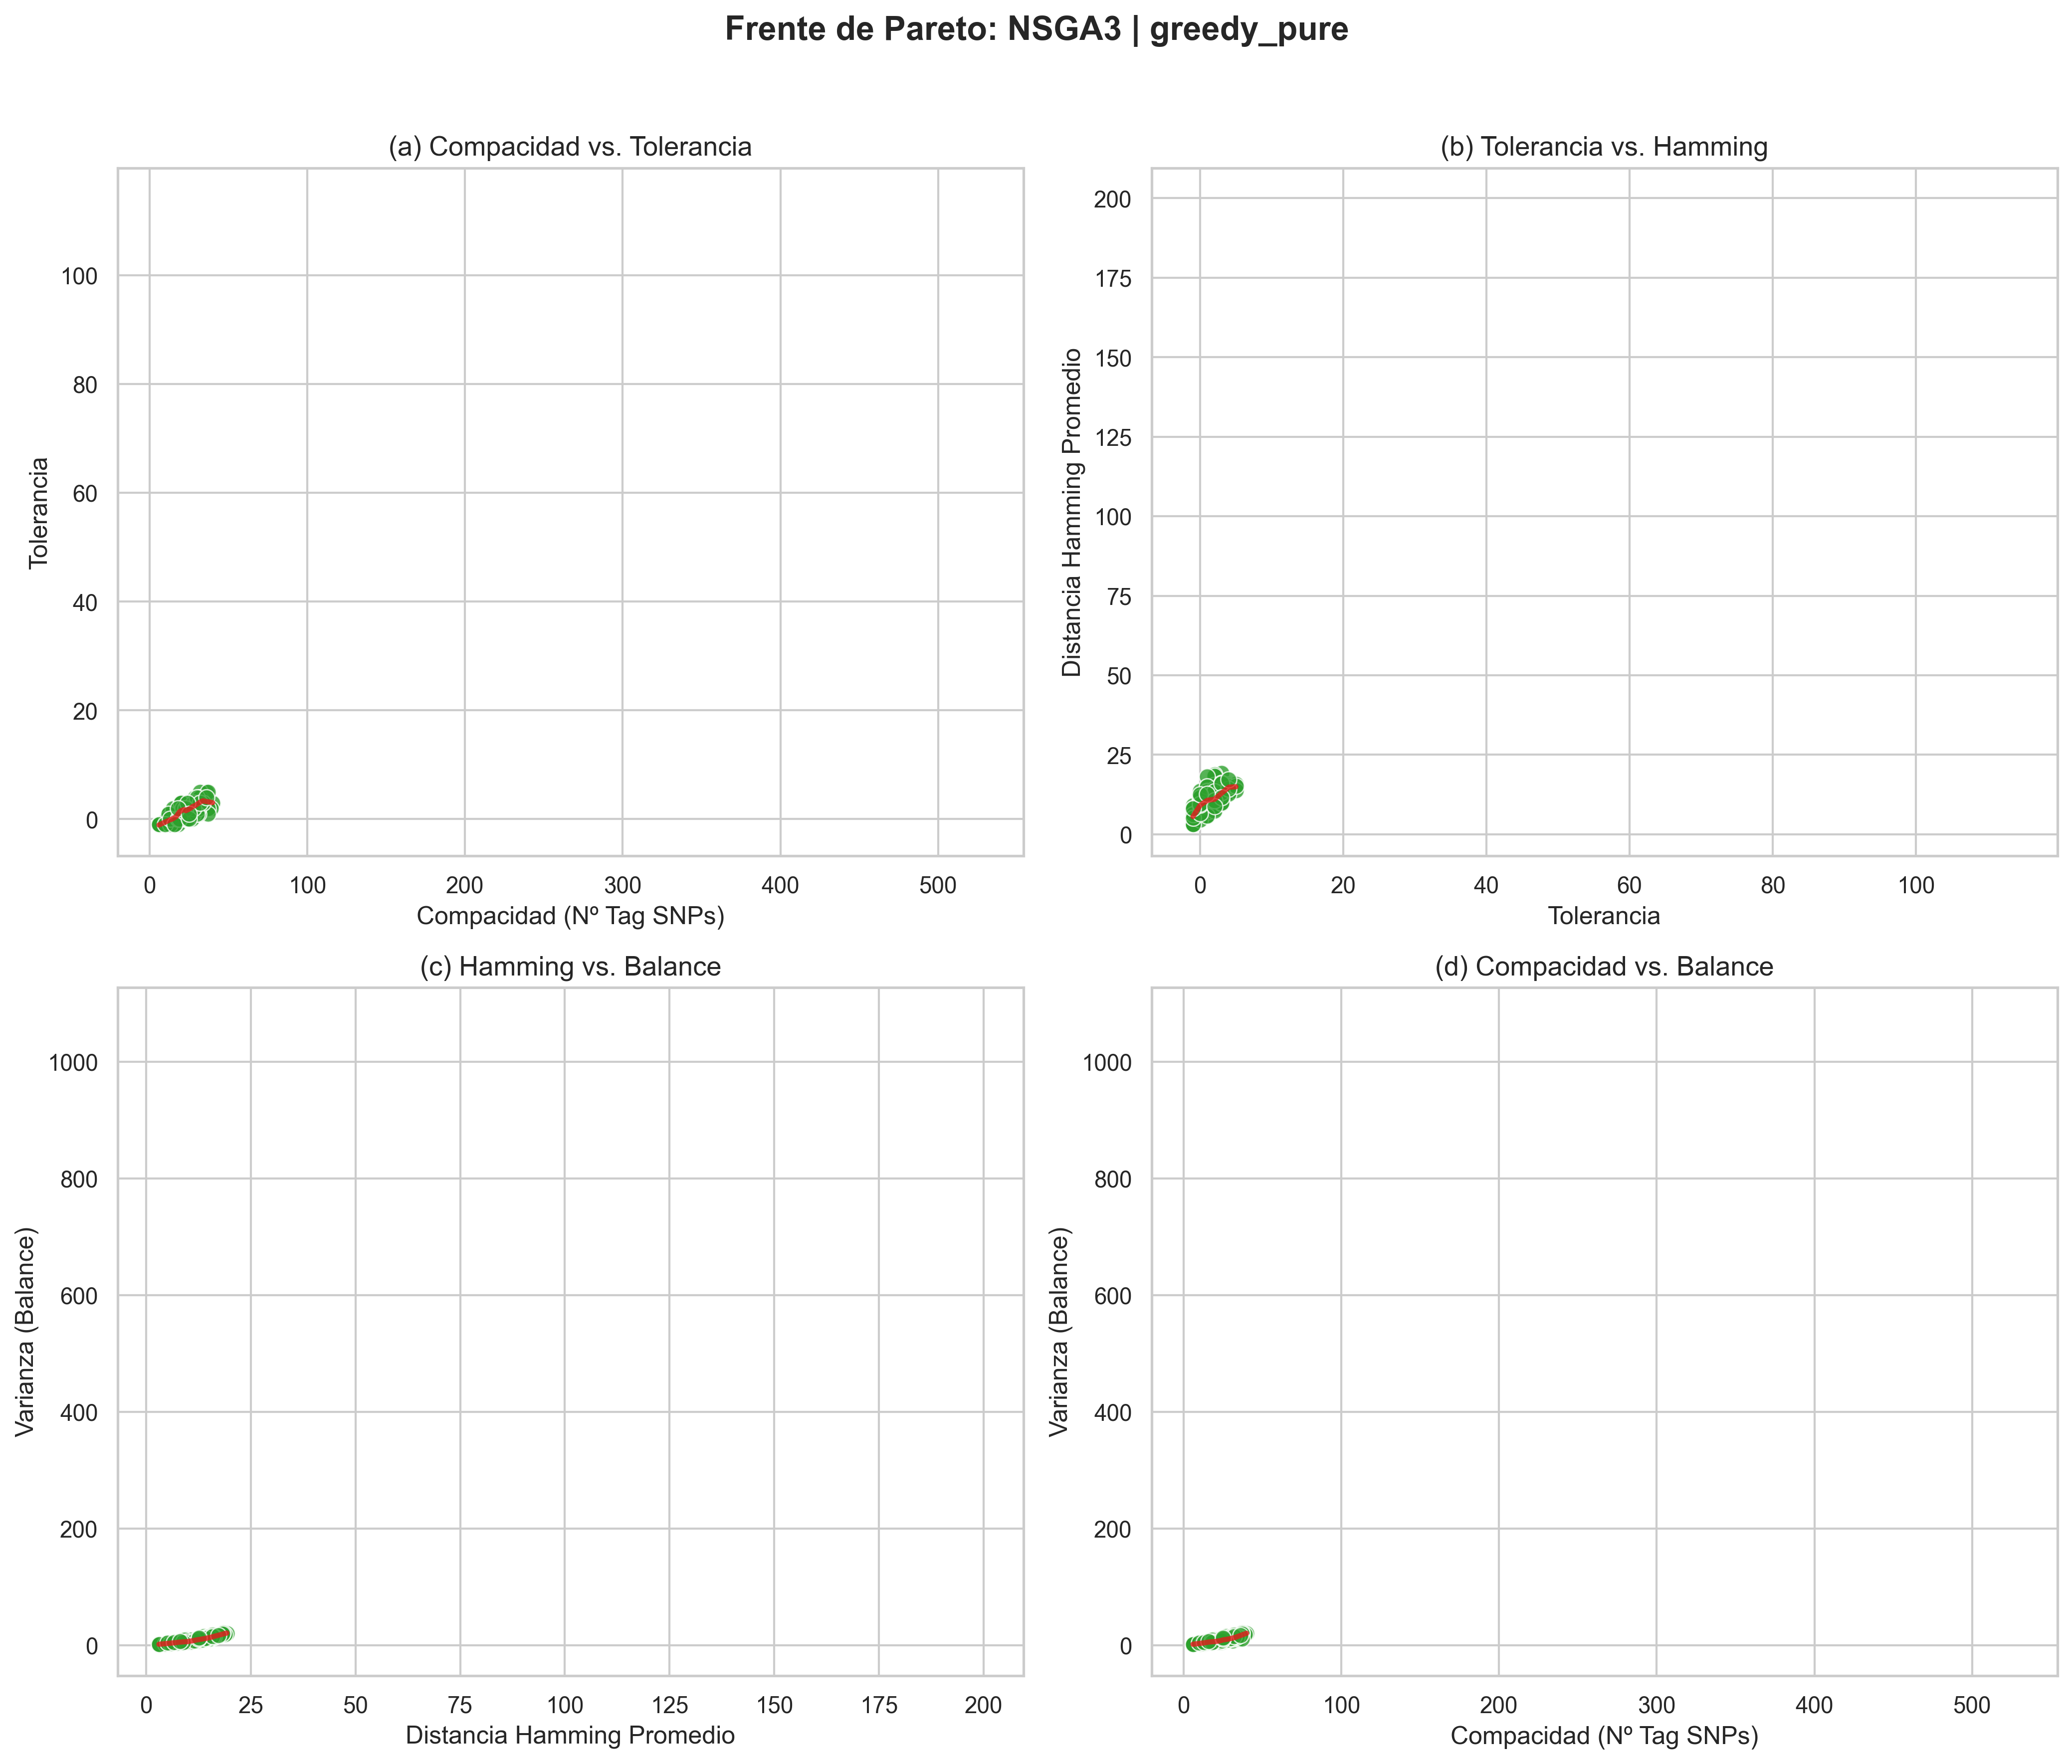
\includegraphics[width=\linewidth]{analisis_assets/20260420T205406/2_comparativa/1_frentes/frentes_pareto/frentes_pareto_nsga3_greedy_pure_full.png} & 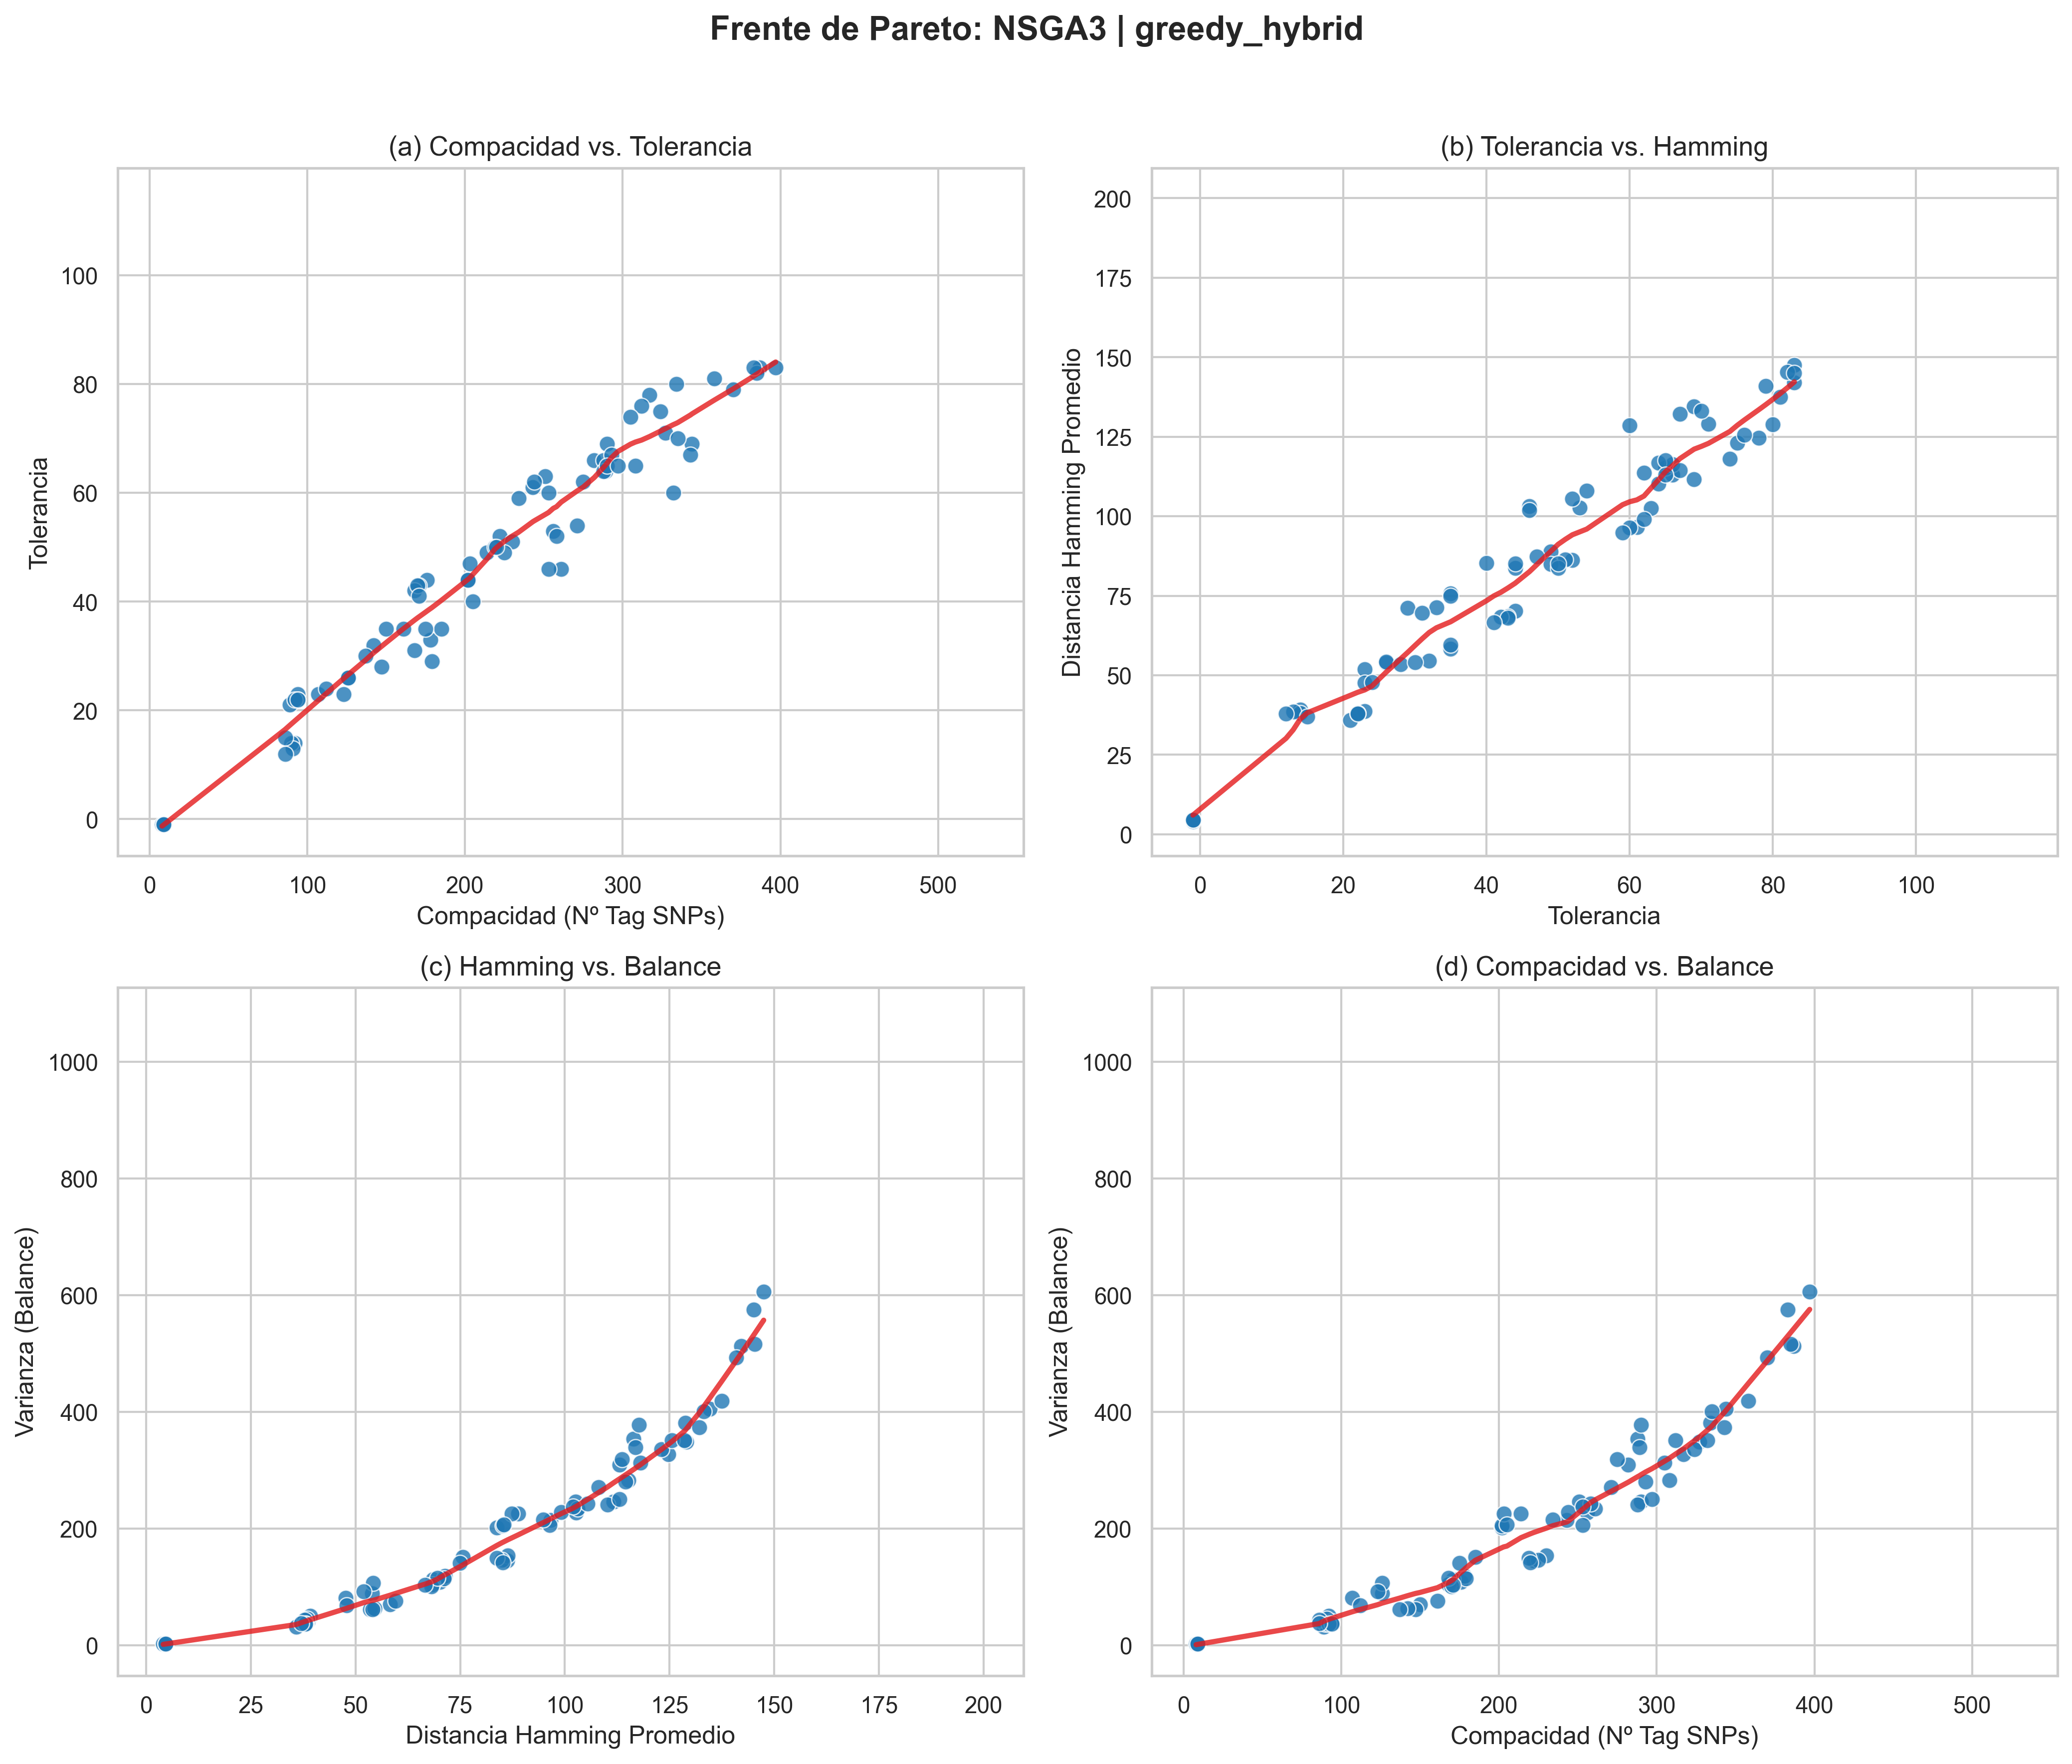
\includegraphics[width=\linewidth]{analisis_assets/20260420T205406/2_comparativa/1_frentes/frentes_pareto/frentes_pareto_nsga3_greedy_hybrid_full.png} \\
        \textbf{SPEA2} & 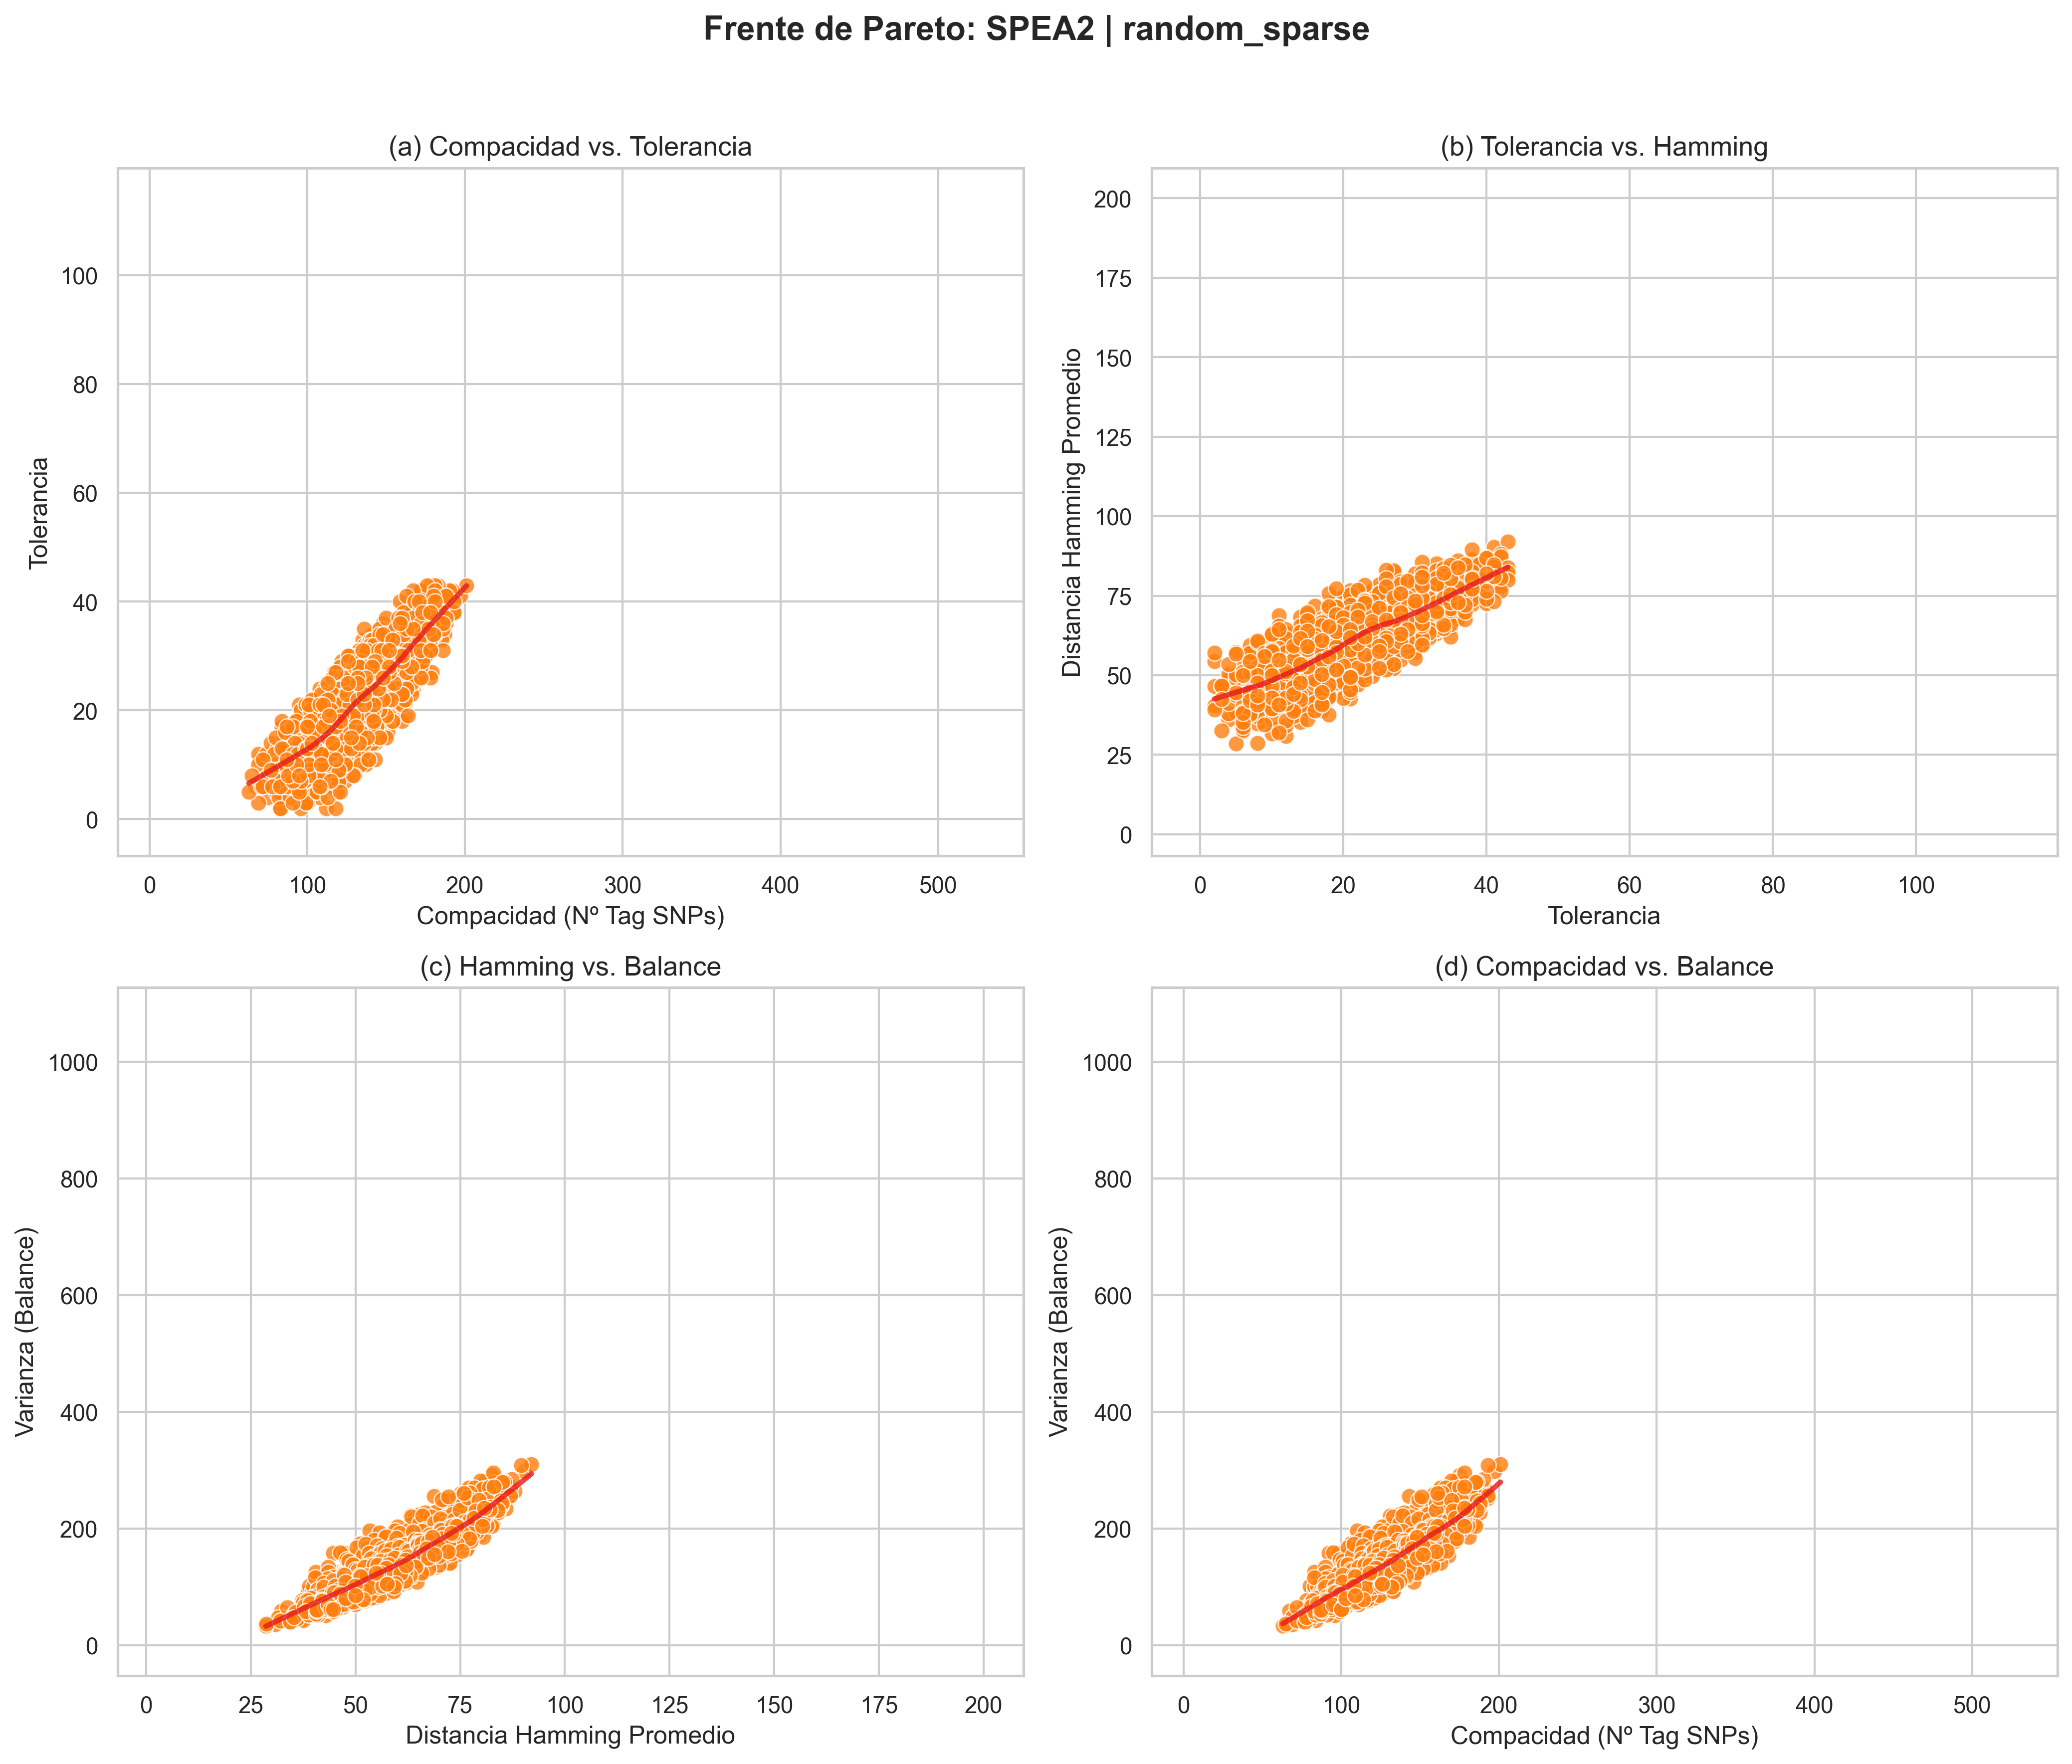
\includegraphics[width=\linewidth]{analisis_assets/20260420T205406/2_comparativa/1_frentes/frentes_pareto/frentes_pareto_spea2_random_sparse_full.png} & 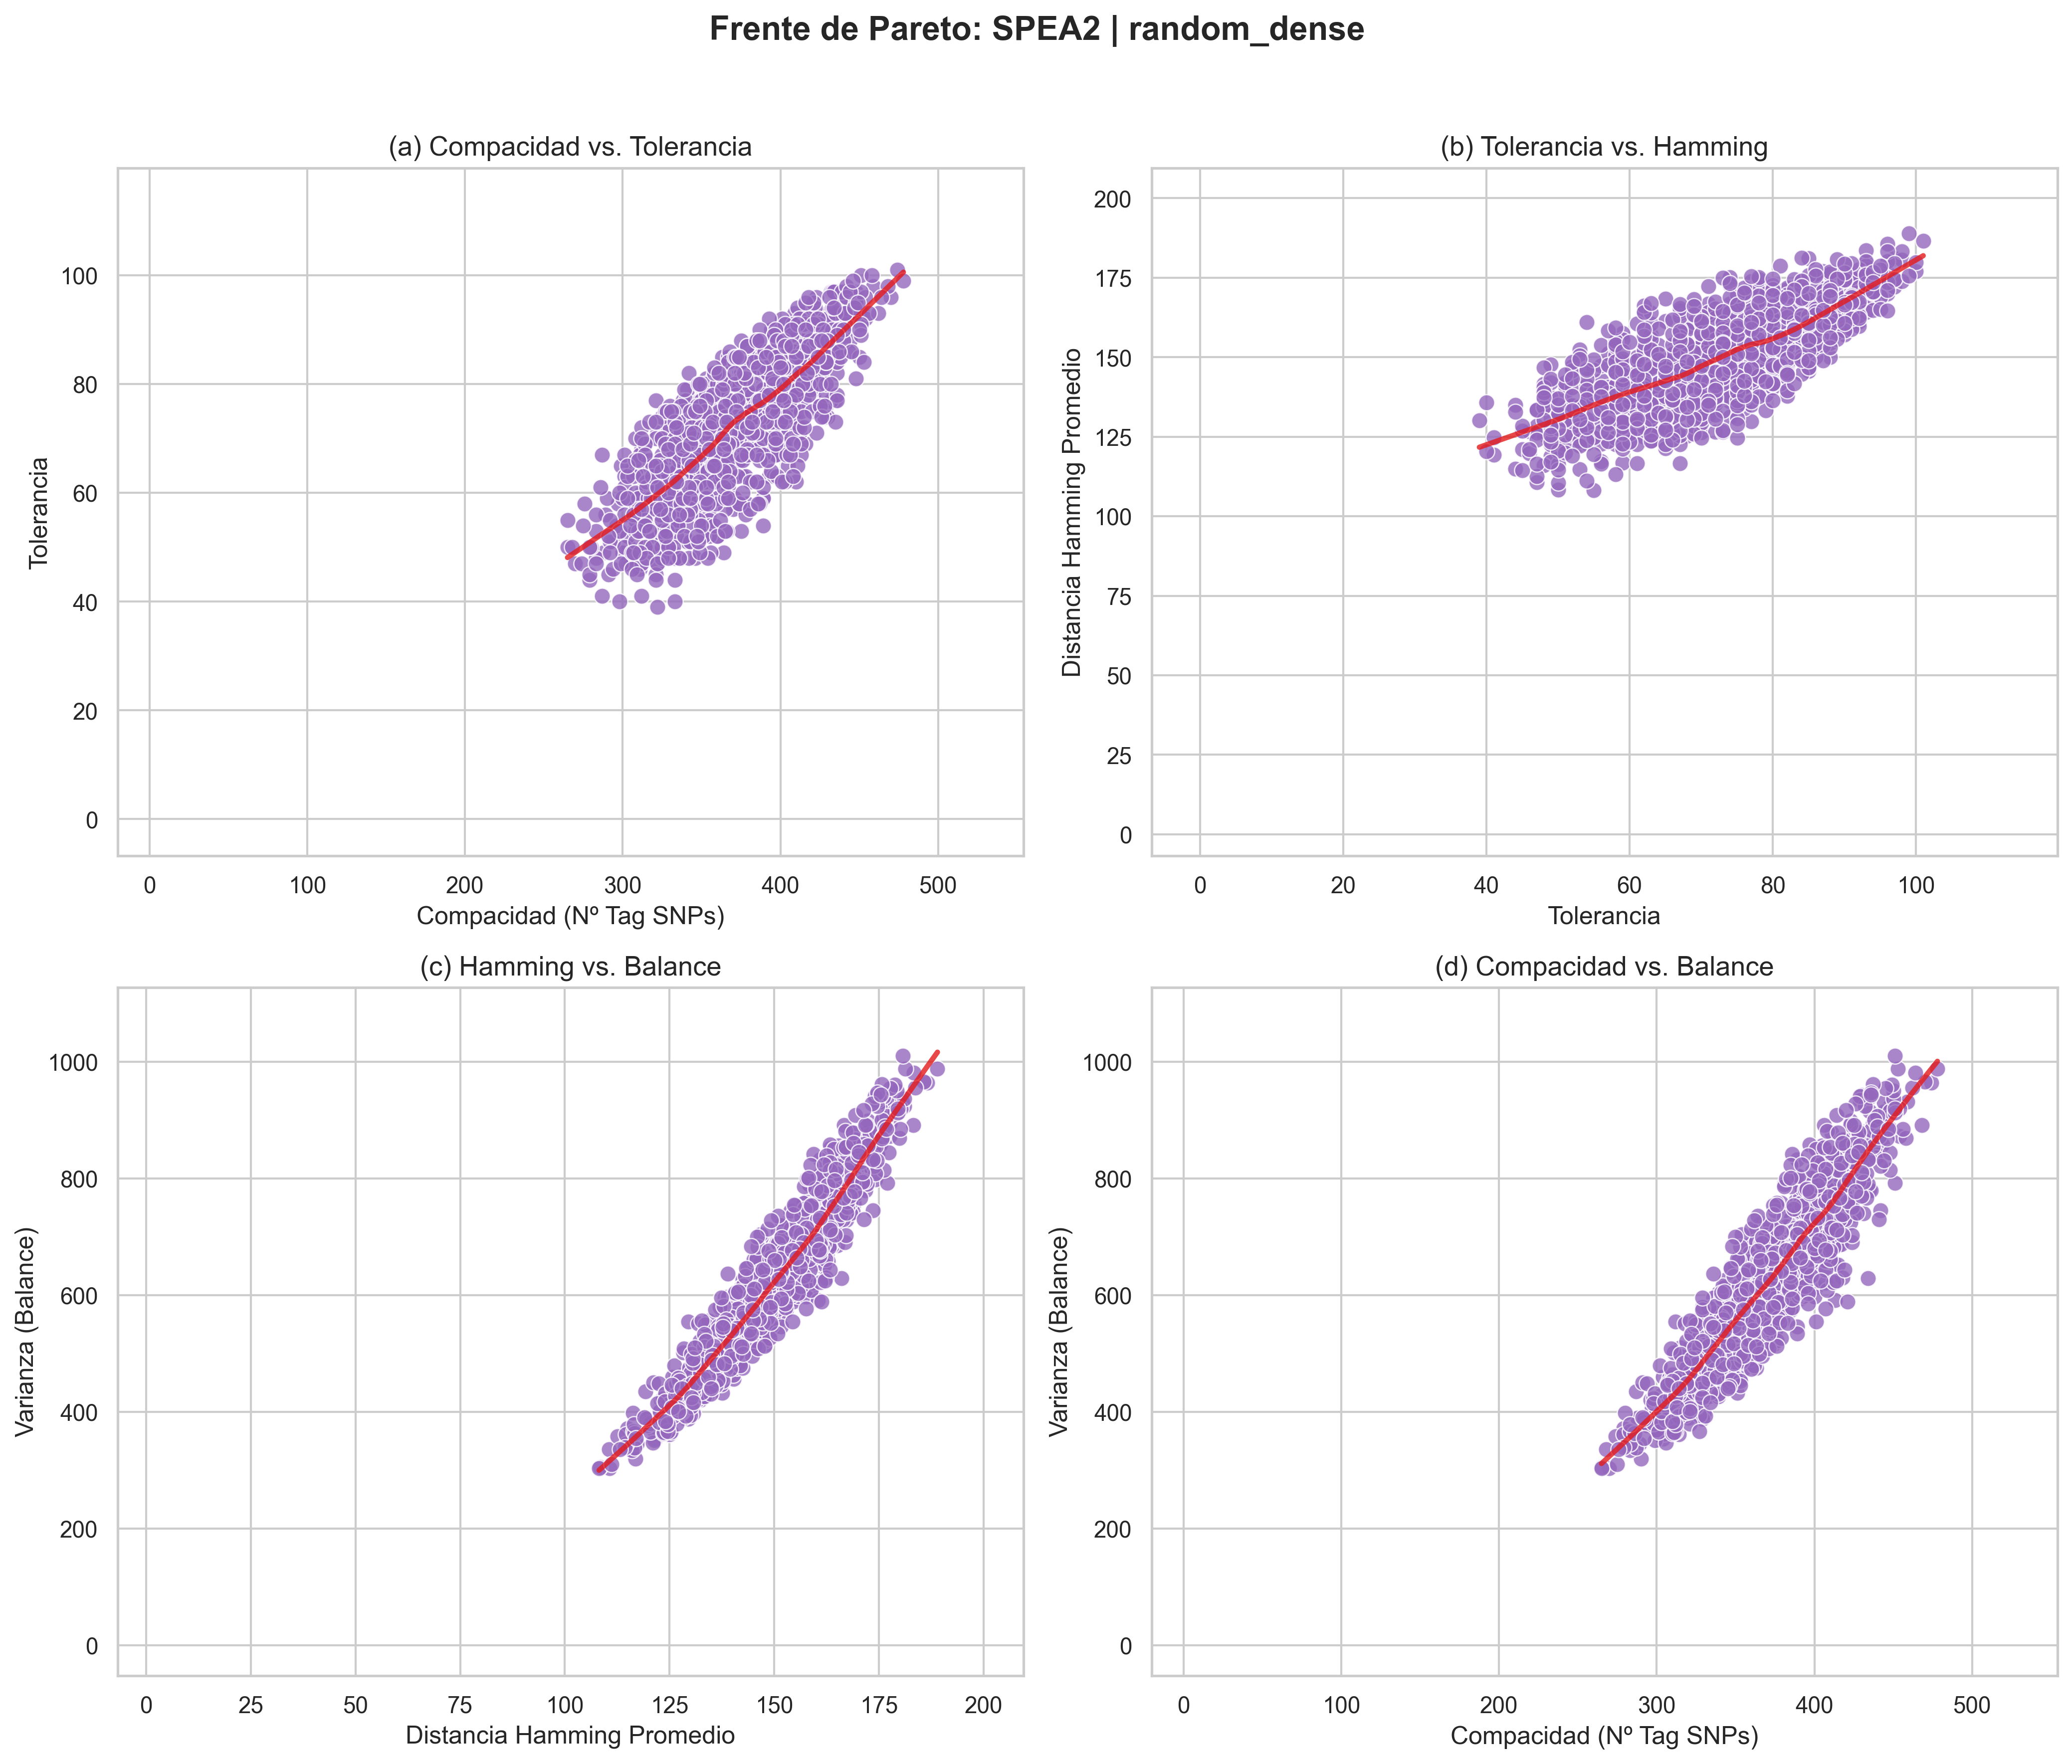
\includegraphics[width=\linewidth]{analisis_assets/20260420T205406/2_comparativa/1_frentes/frentes_pareto/frentes_pareto_spea2_random_dense_full.png} & 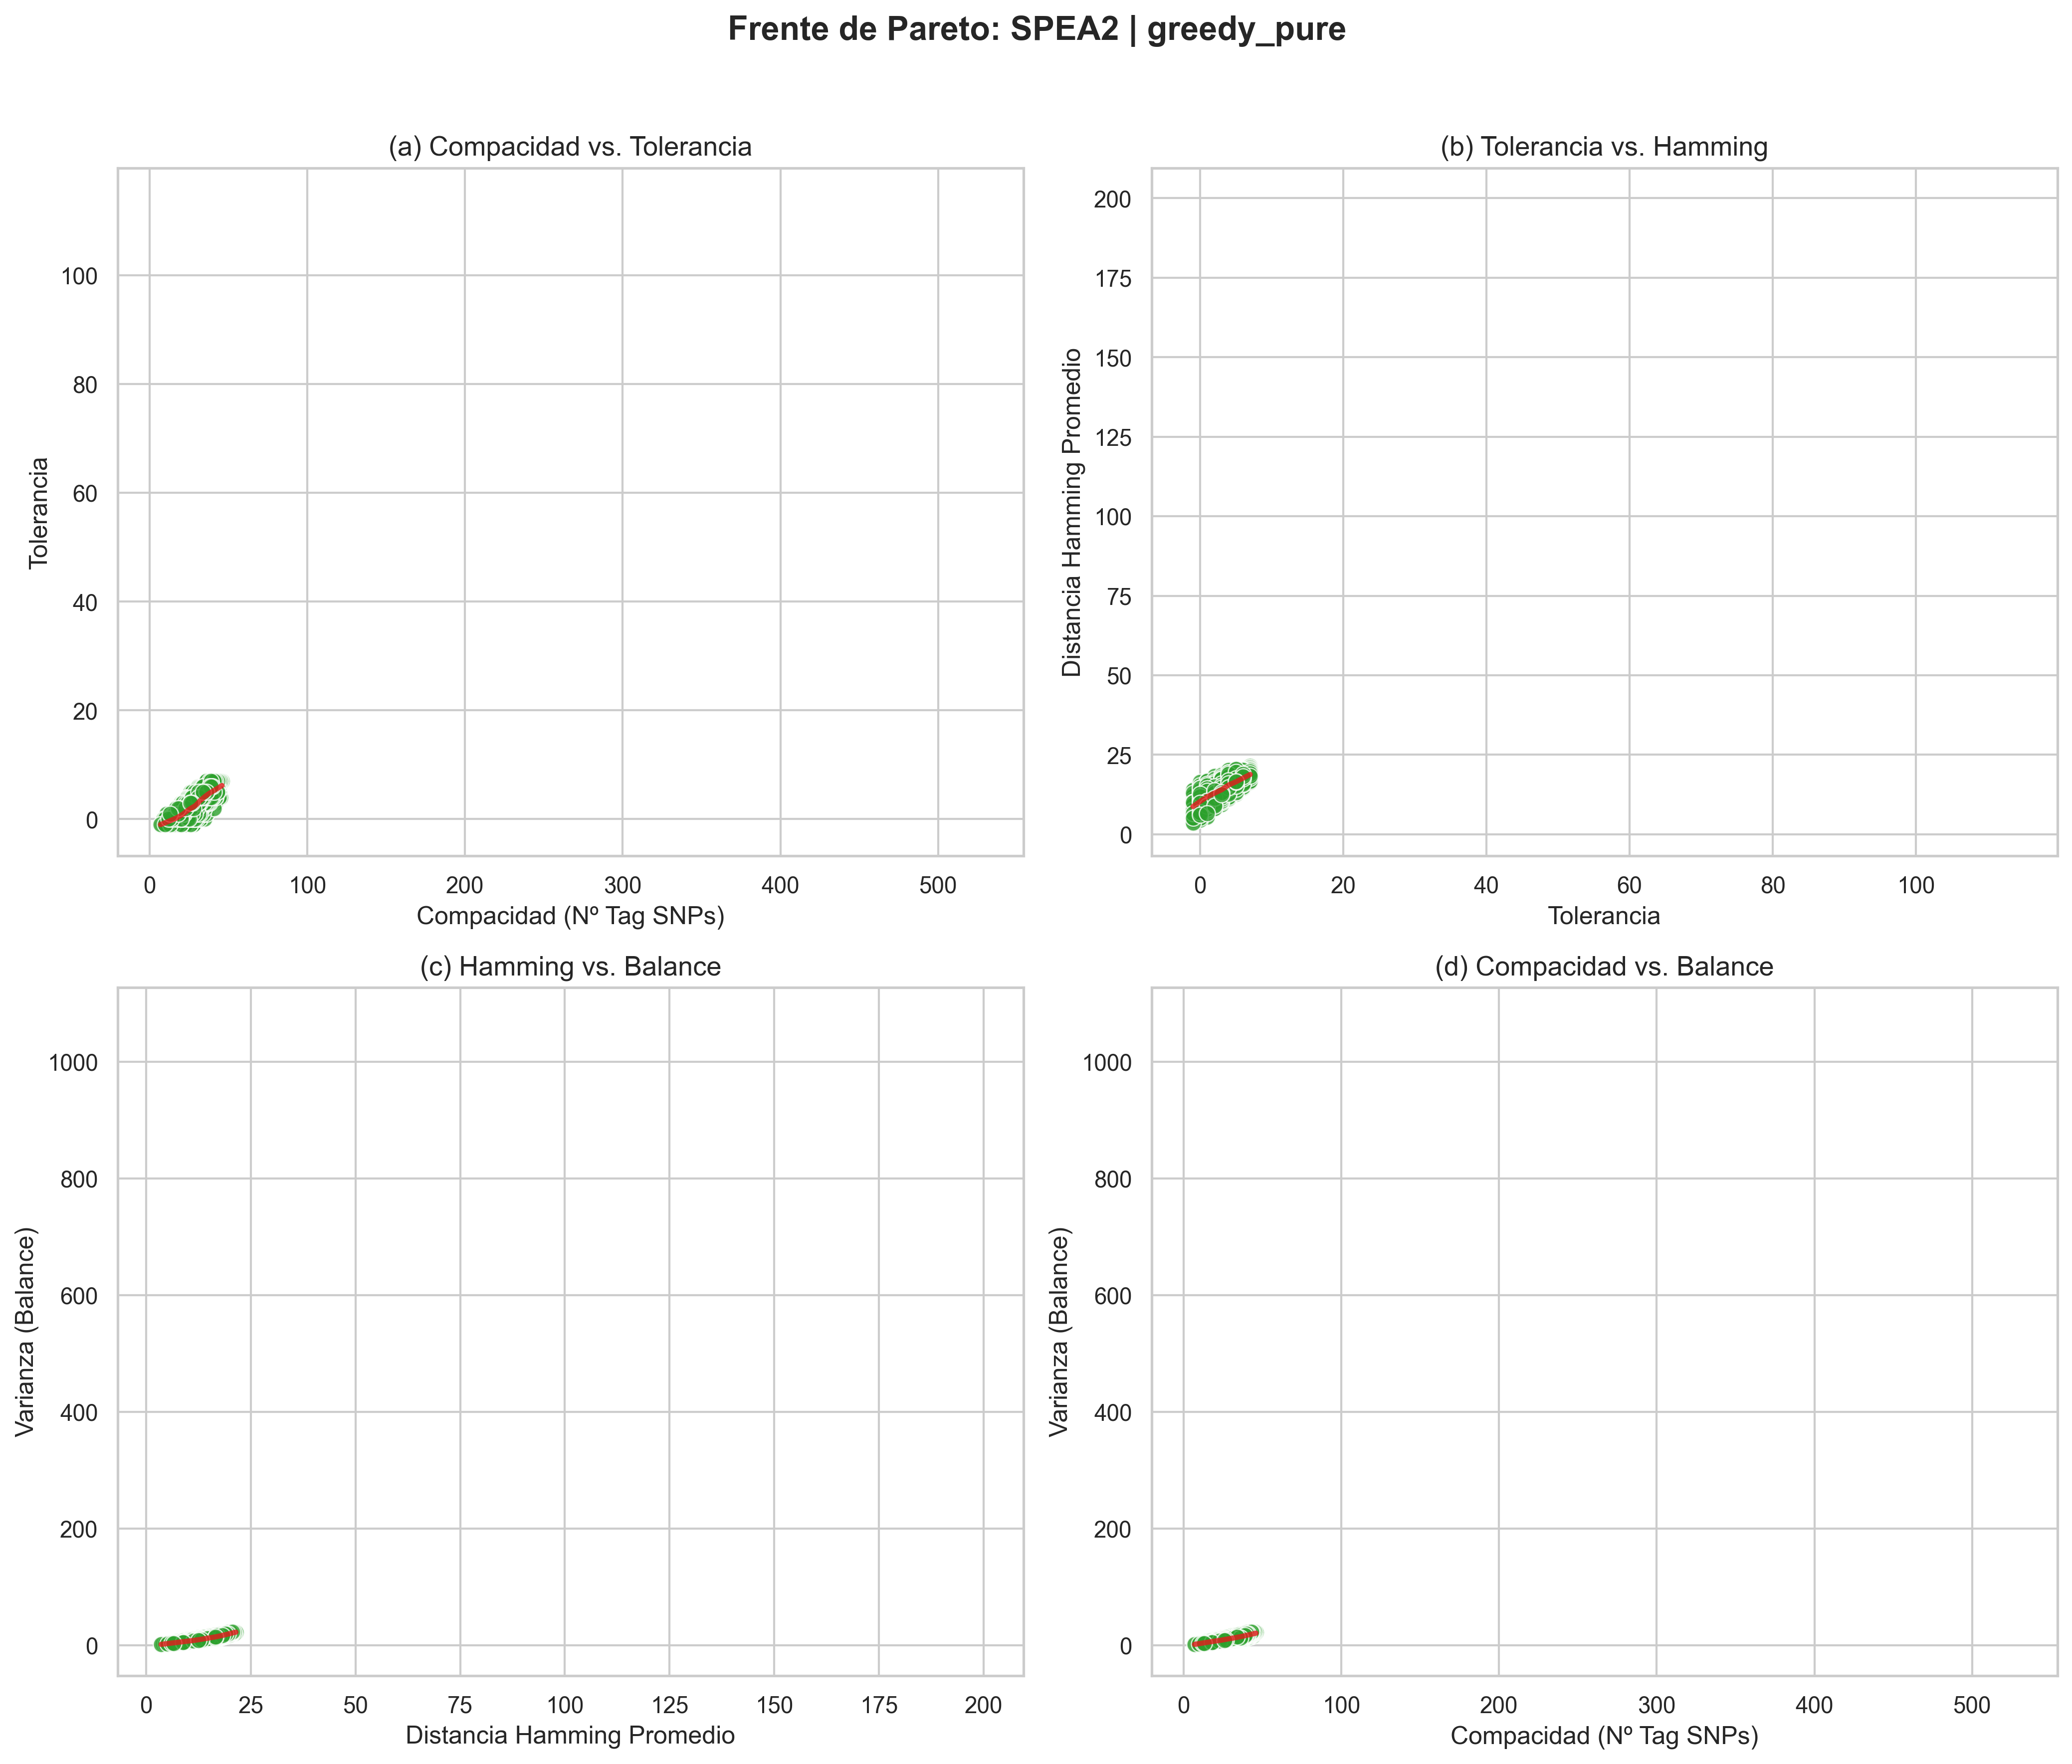
\includegraphics[width=\linewidth]{analisis_assets/20260420T205406/2_comparativa/1_frentes/frentes_pareto/frentes_pareto_spea2_greedy_pure_full.png} & 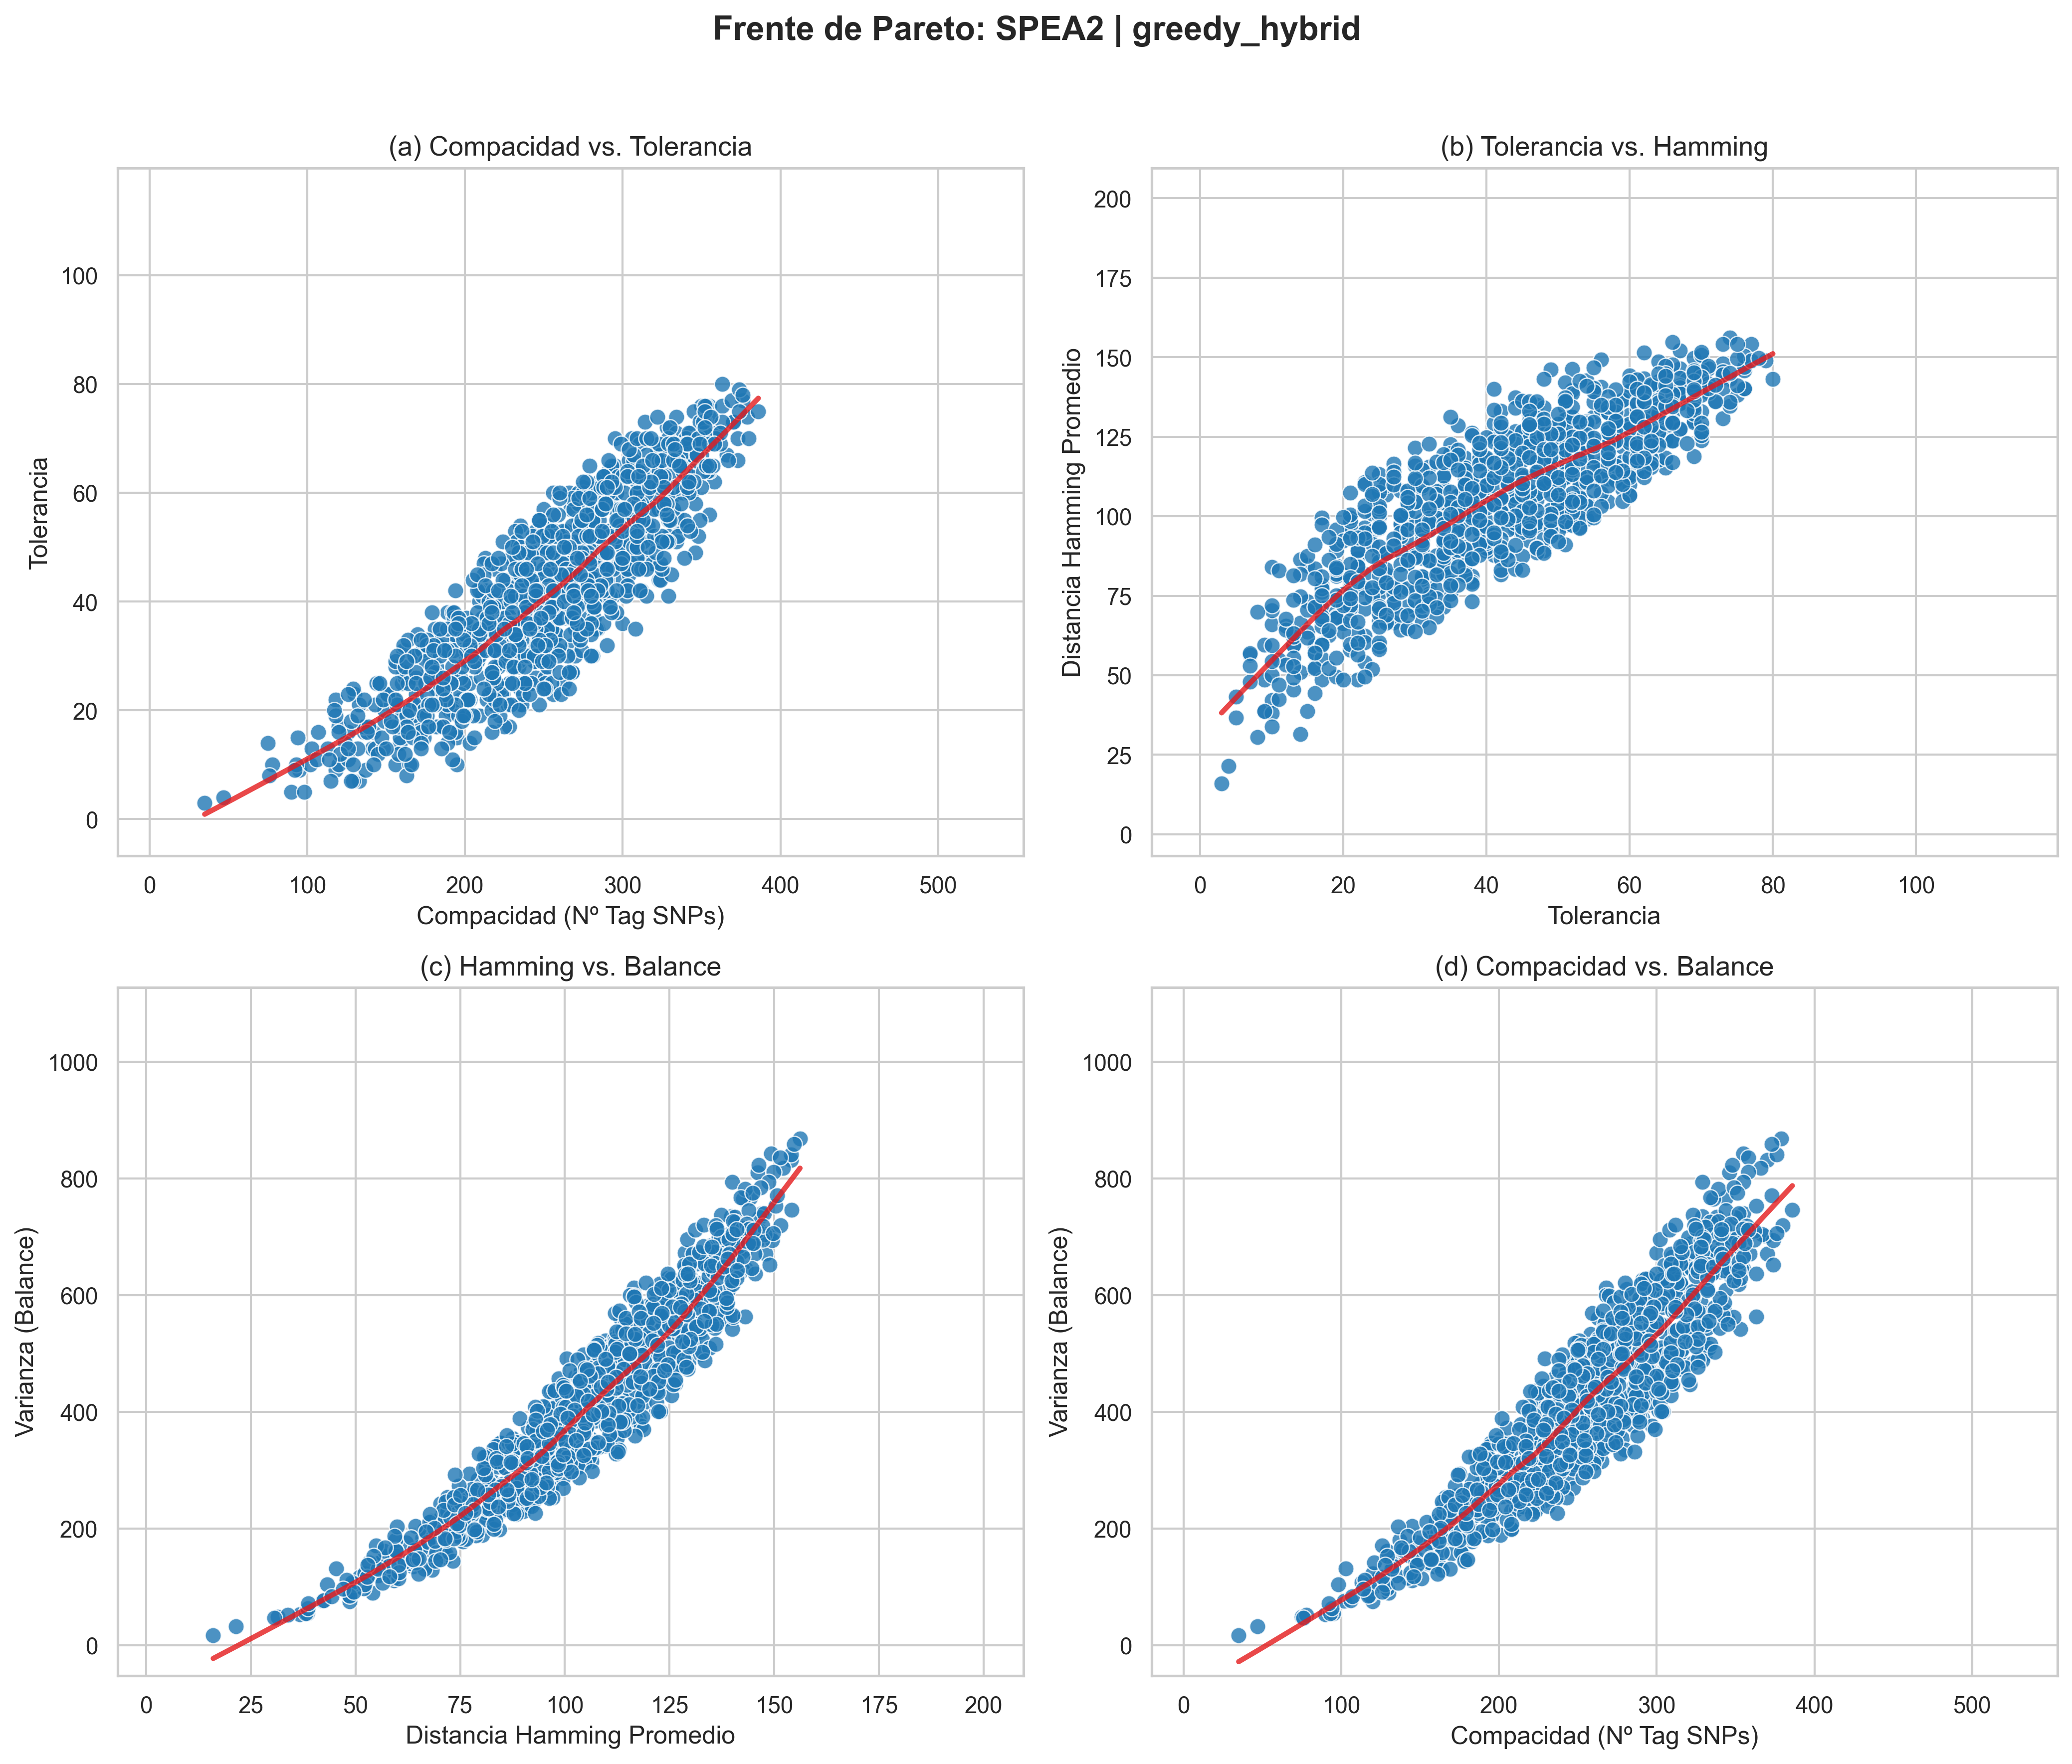
\includegraphics[width=\linewidth]{analisis_assets/20260420T205406/2_comparativa/1_frentes/frentes_pareto/frentes_pareto_spea2_greedy_hybrid_full.png} \\
        \textbf{MOEA/D (PBI)} & 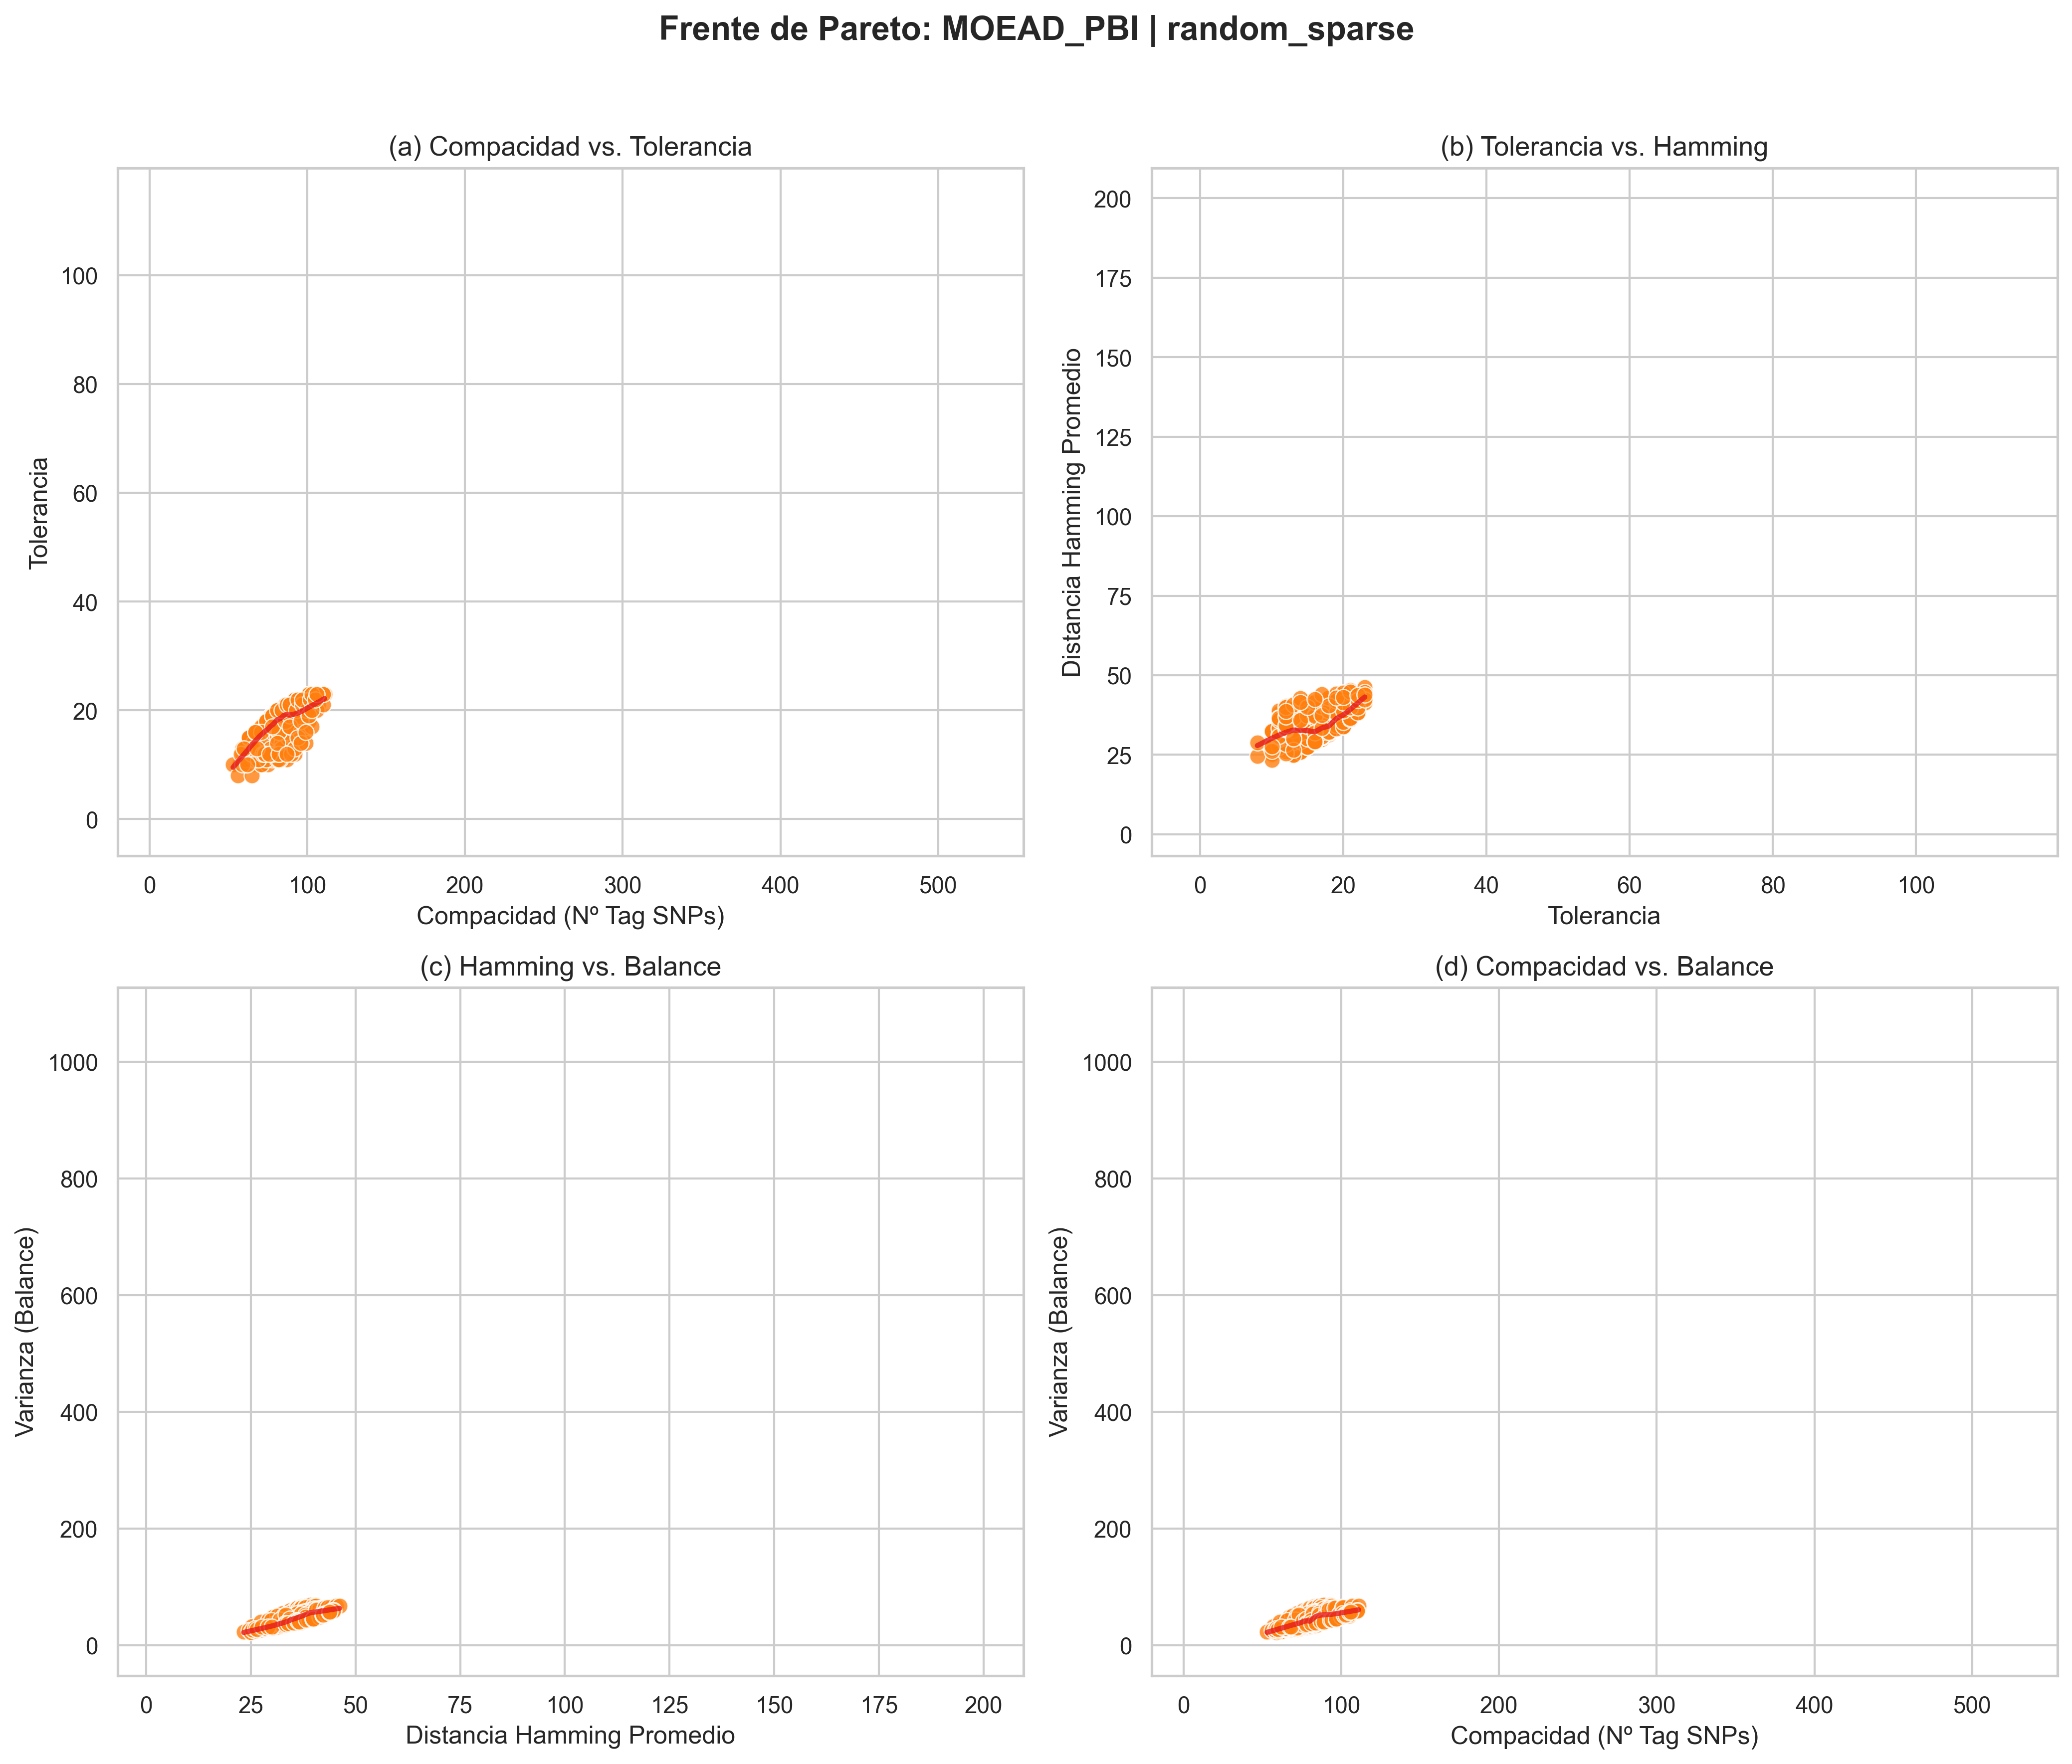
\includegraphics[width=\linewidth]{analisis_assets/20260420T205406/2_comparativa/1_frentes/frentes_pareto/frentes_pareto_moead_pbi_random_sparse_full.png} & 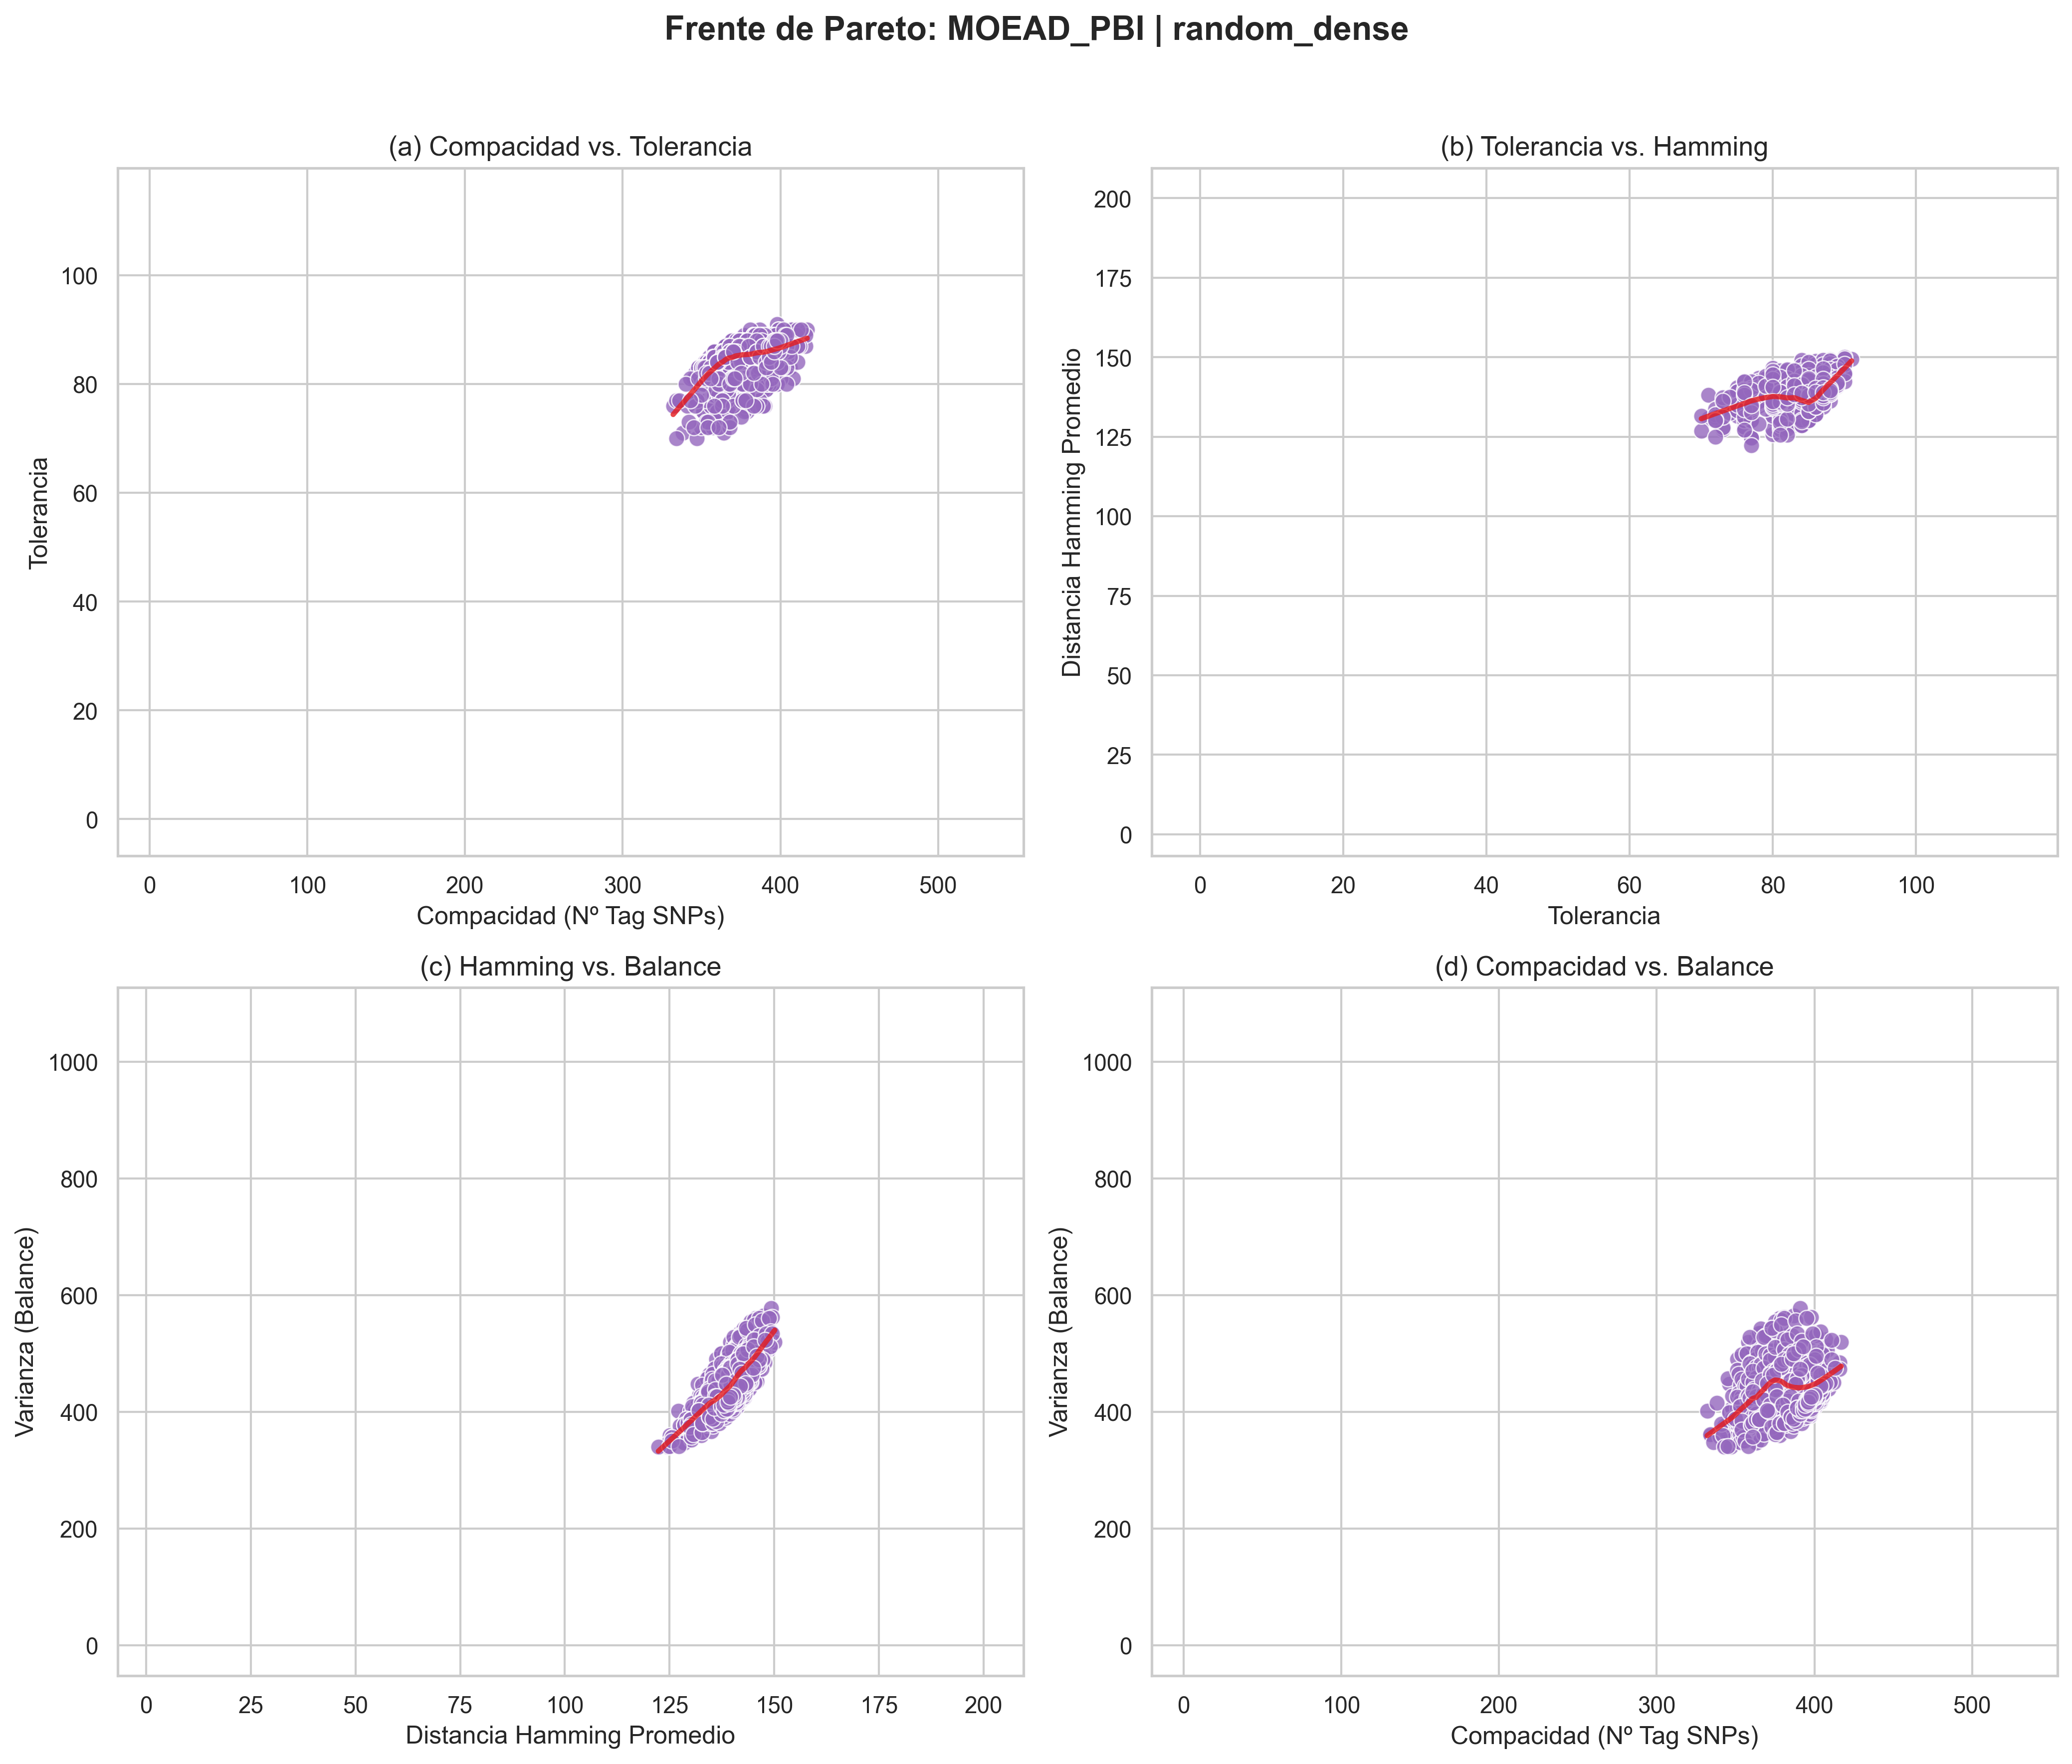
\includegraphics[width=\linewidth]{analisis_assets/20260420T205406/2_comparativa/1_frentes/frentes_pareto/frentes_pareto_moead_pbi_random_dense_full.png} & 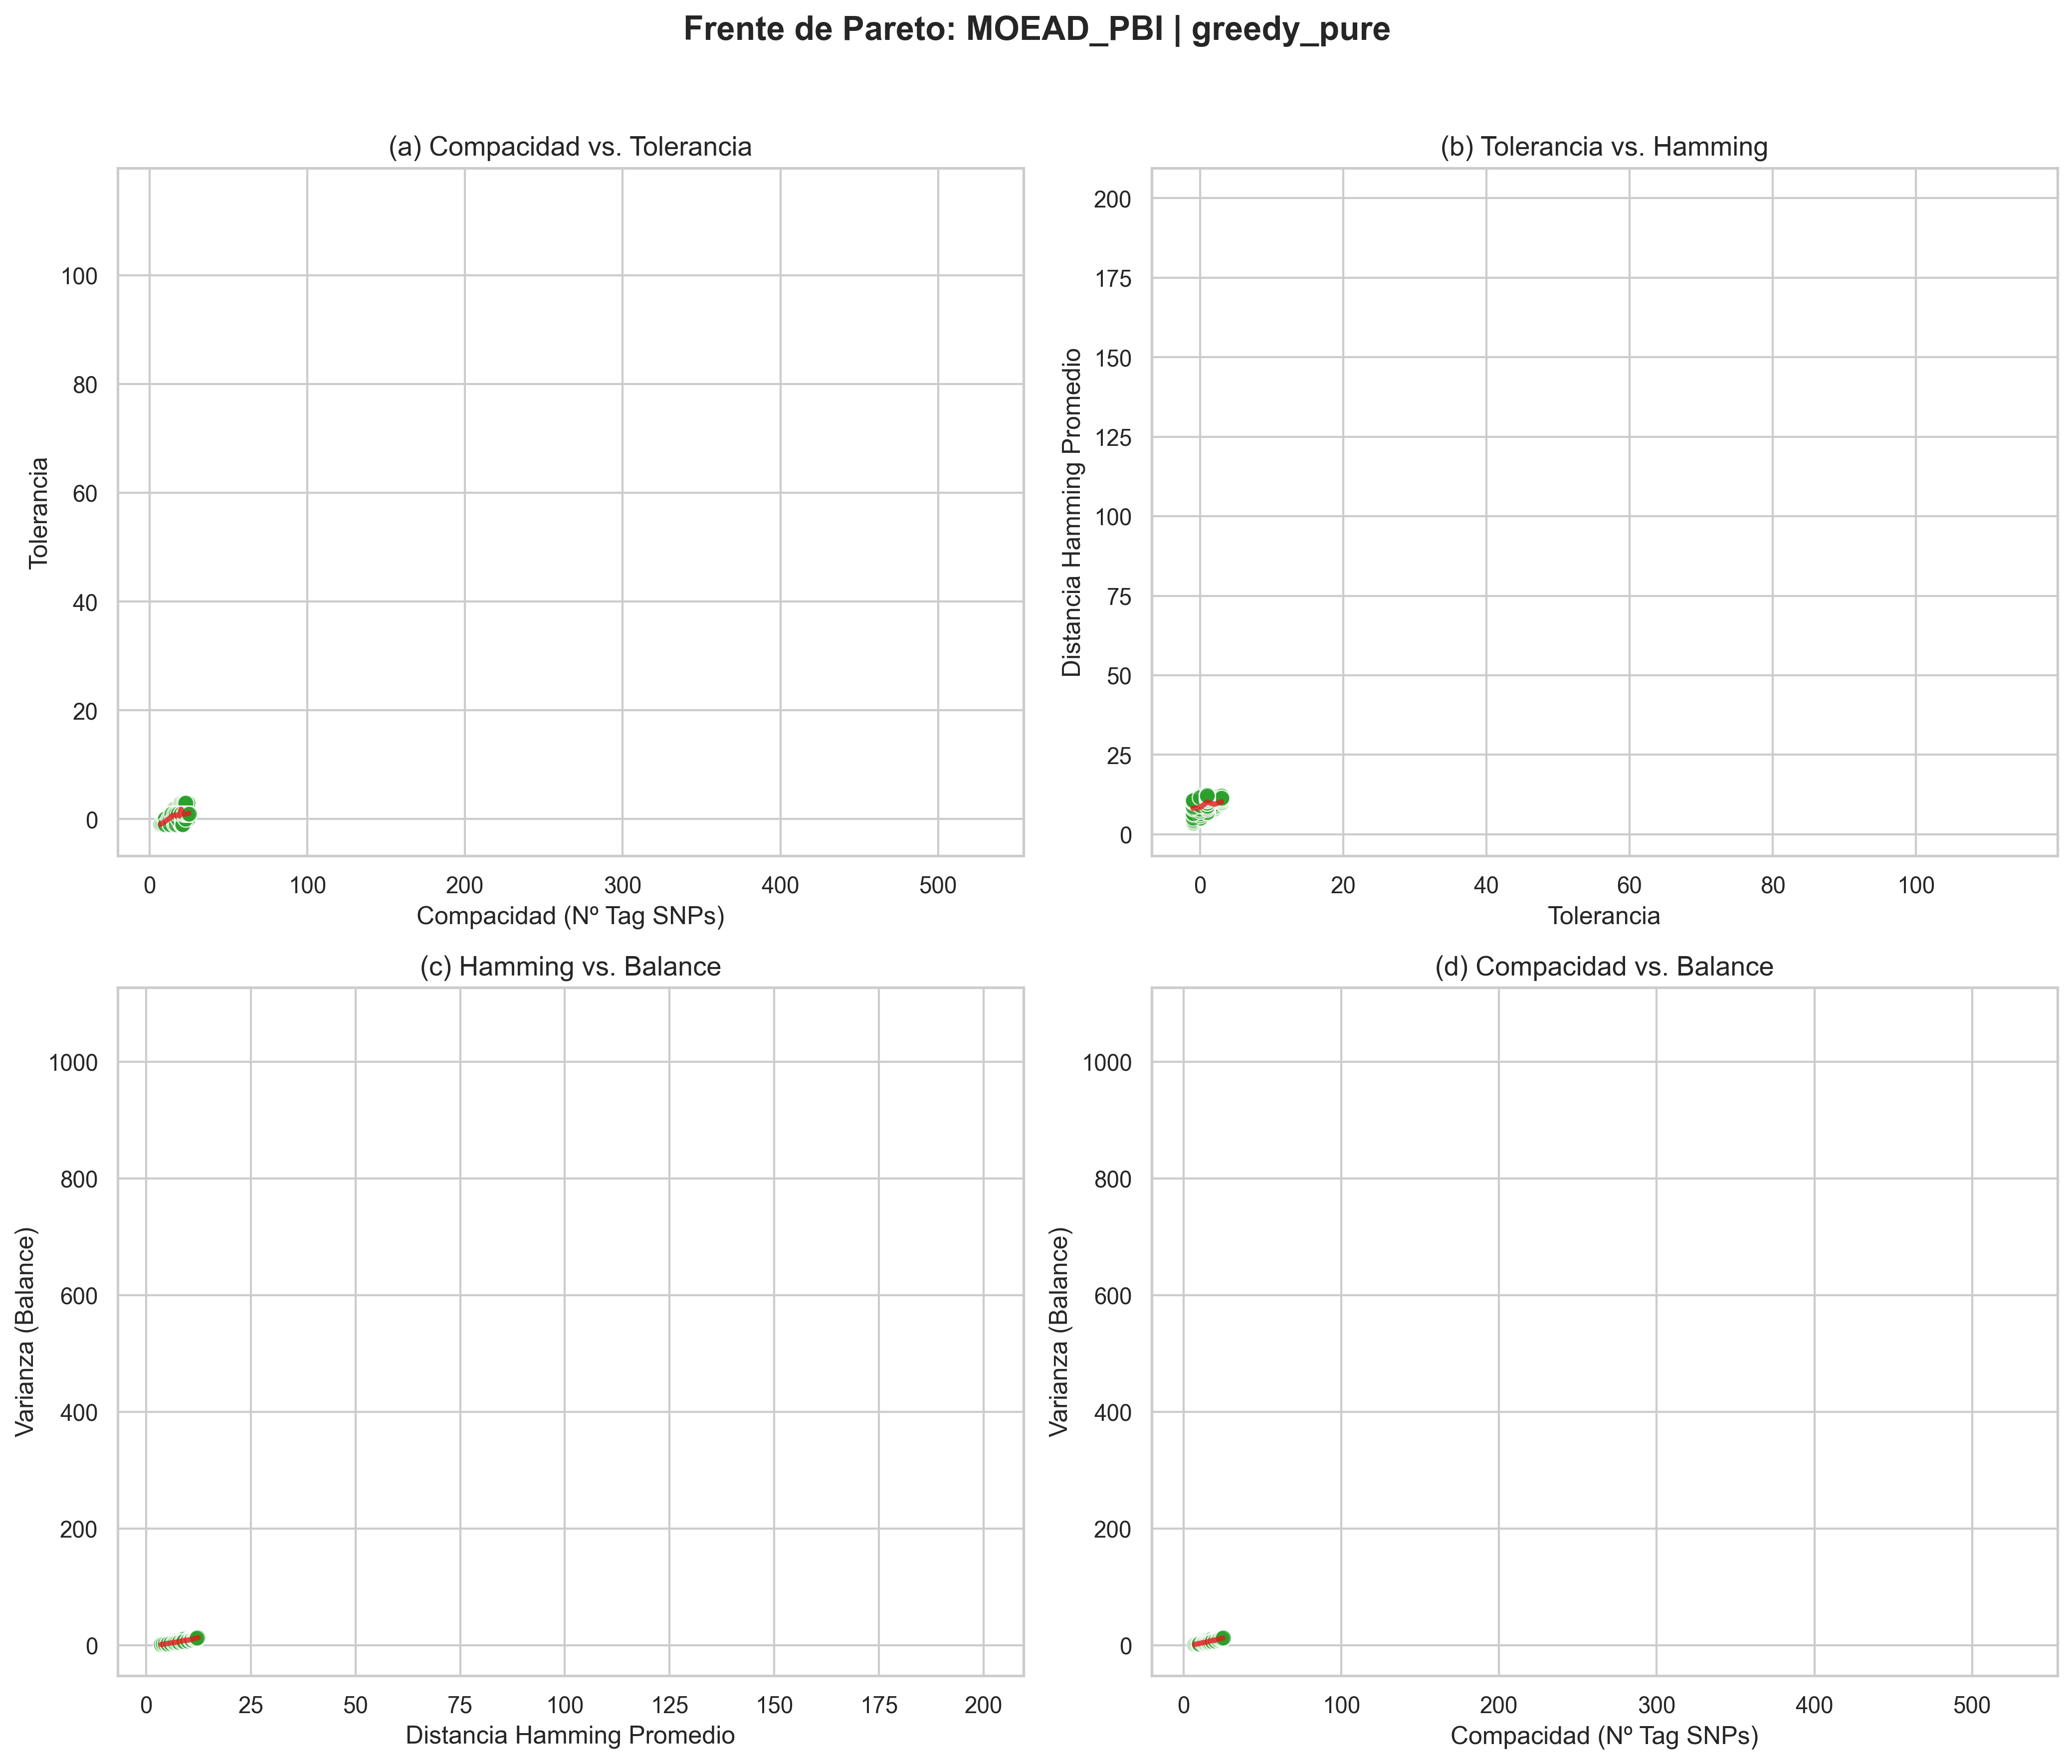
\includegraphics[width=\linewidth]{analisis_assets/20260420T205406/2_comparativa/1_frentes/frentes_pareto/frentes_pareto_moead_pbi_greedy_pure_full.png} & 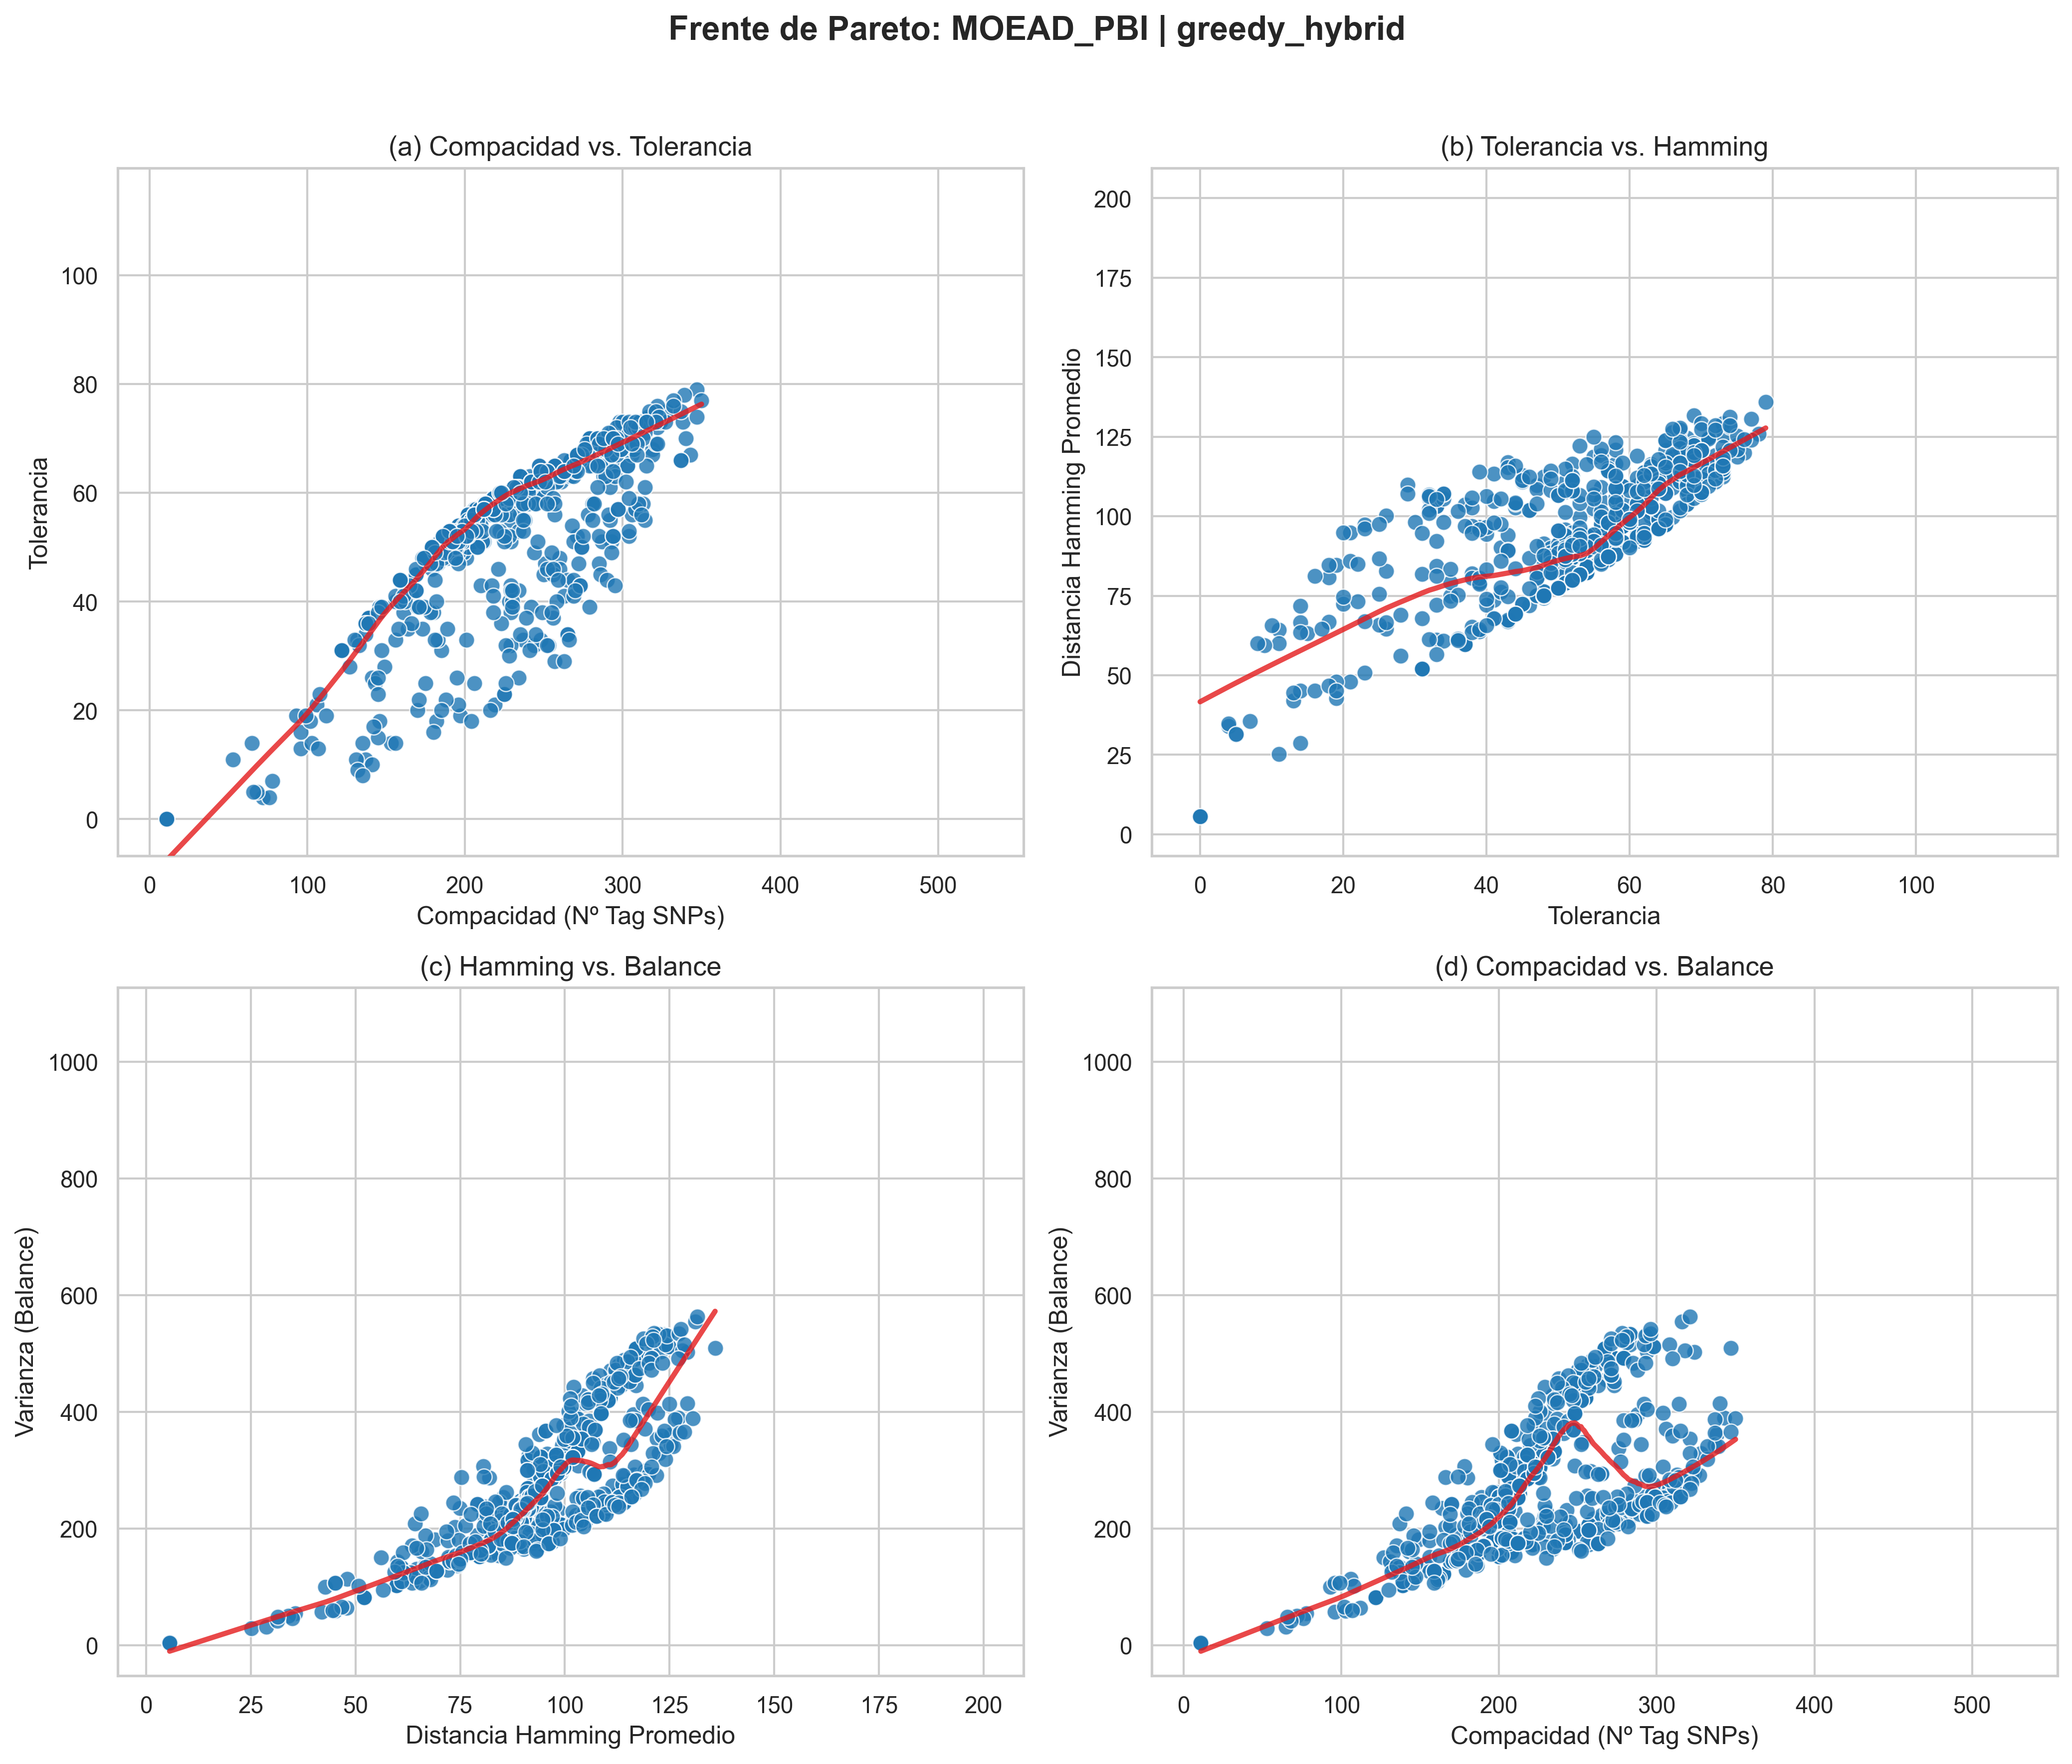
\includegraphics[width=\linewidth]{analisis_assets/20260420T205406/2_comparativa/1_frentes/frentes_pareto/frentes_pareto_moead_pbi_greedy_hybrid_full.png} \\
        \textbf{MOEA/D (TCHE)} & 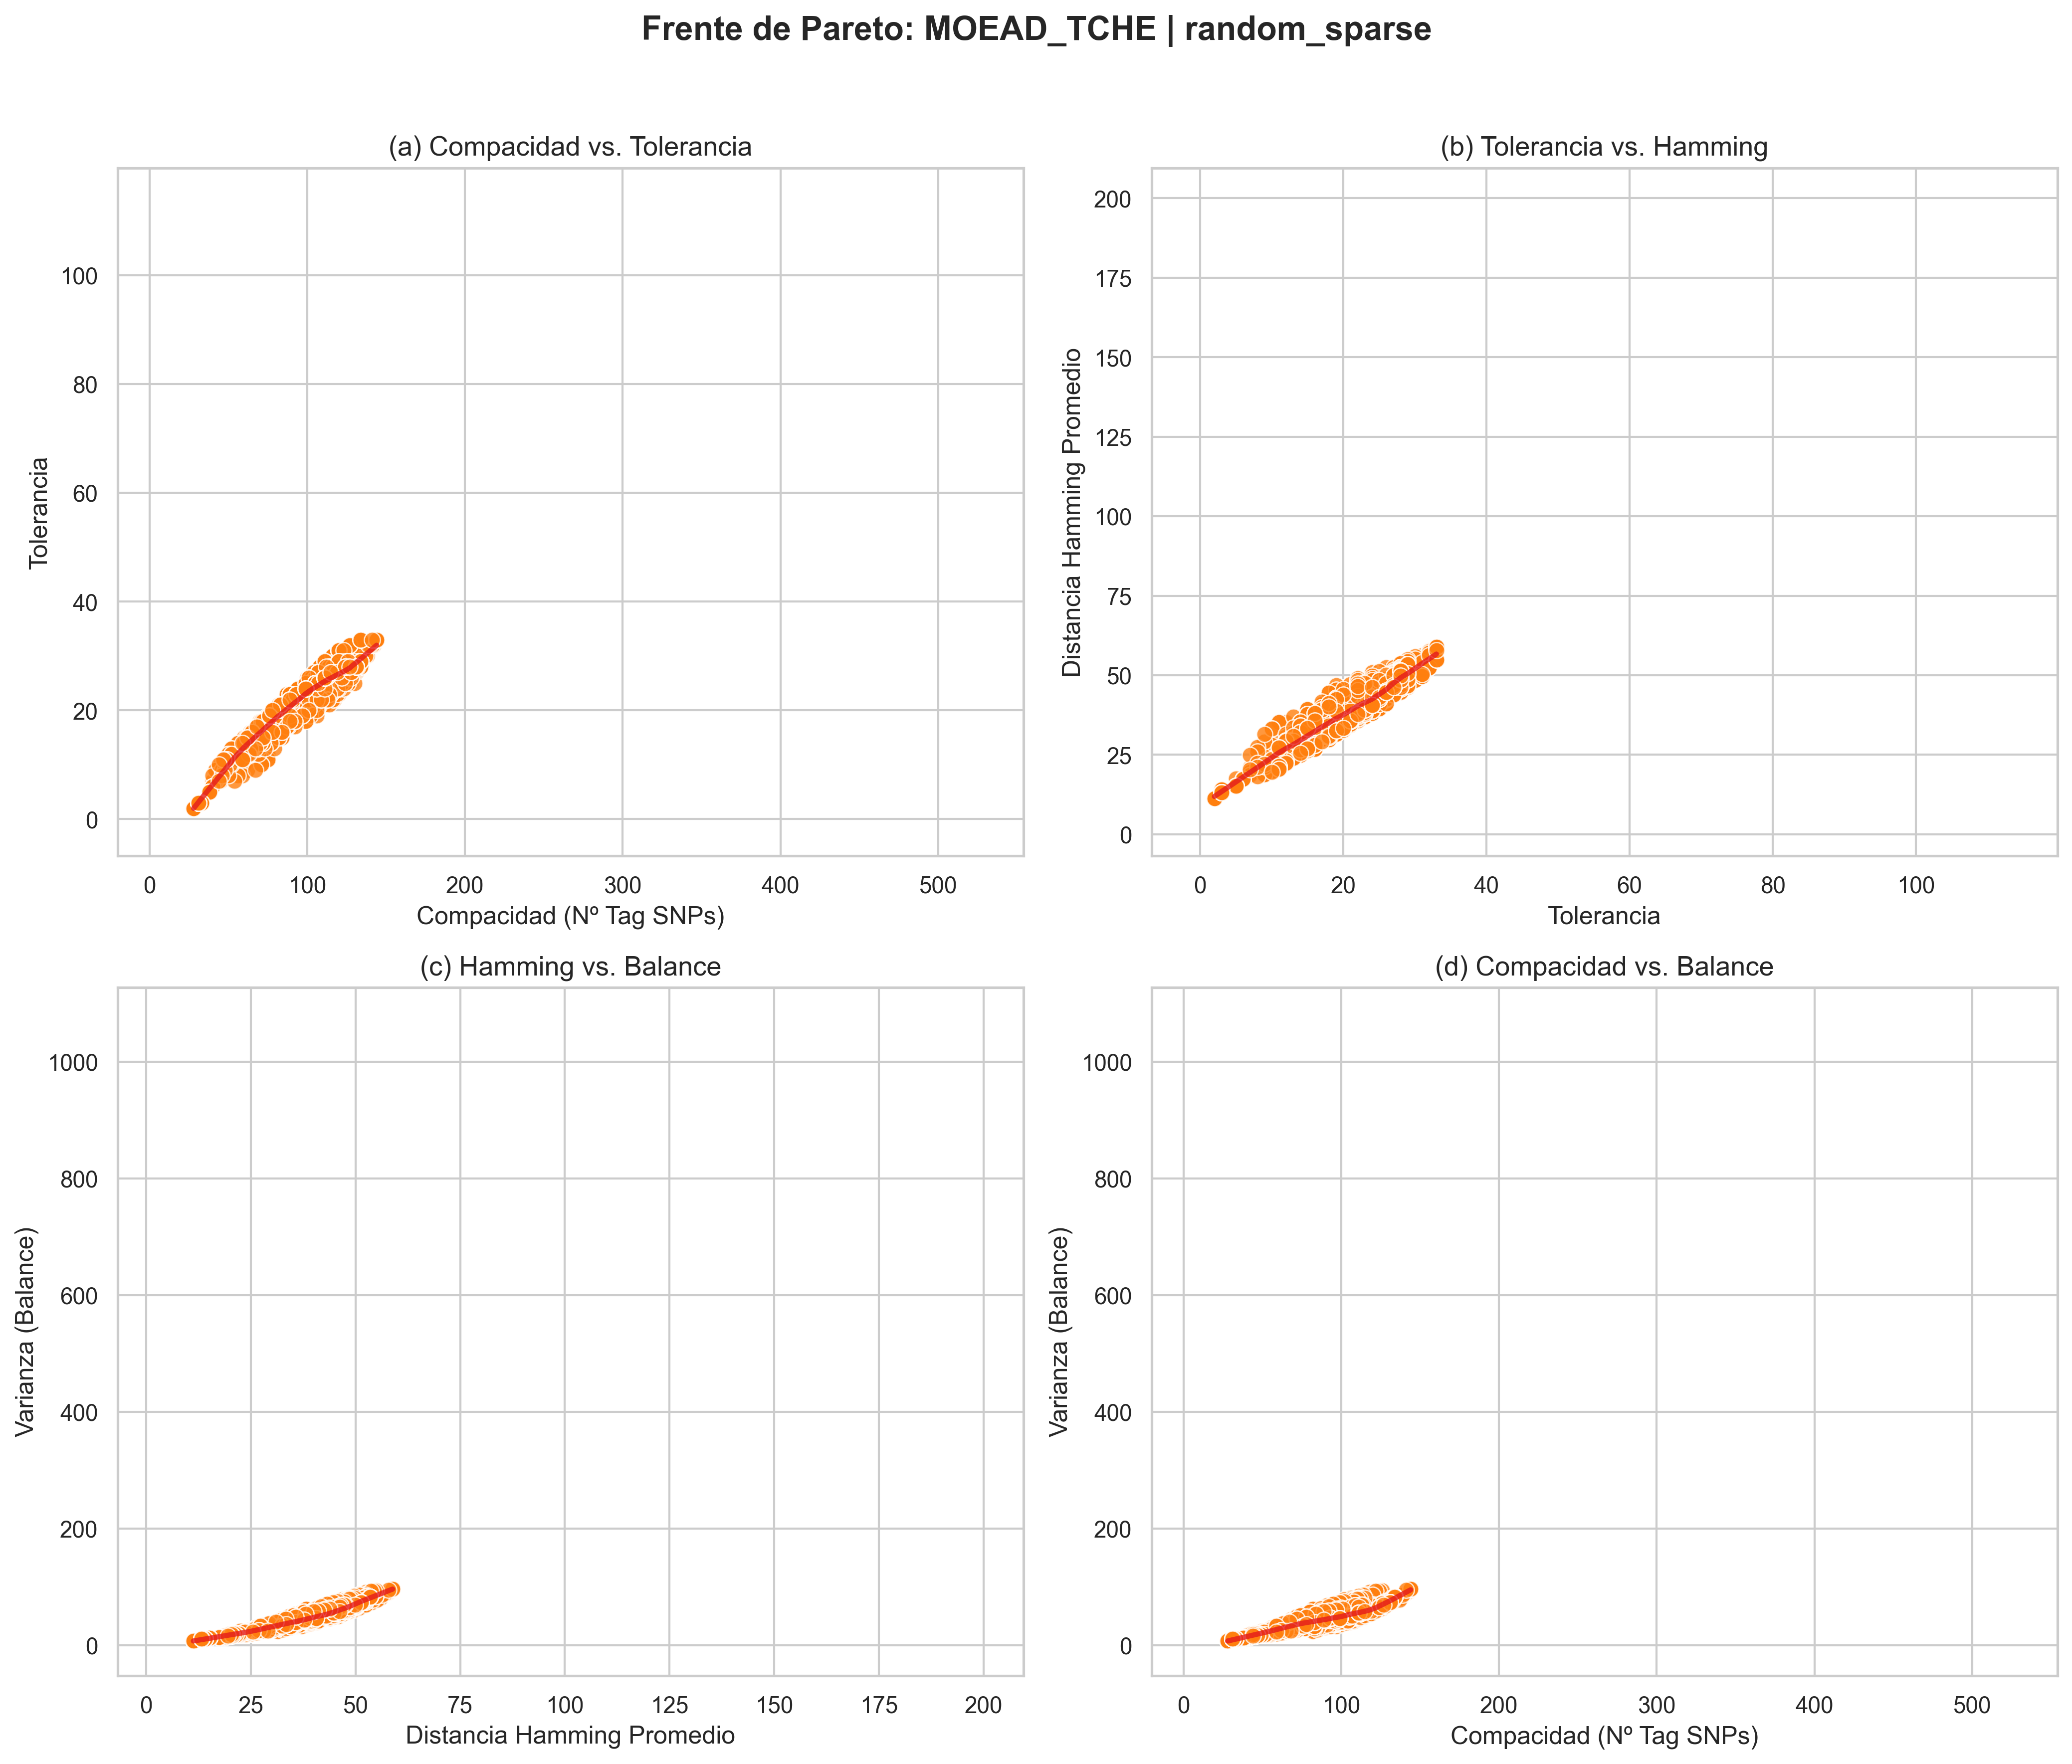
\includegraphics[width=\linewidth]{analisis_assets/20260420T205406/2_comparativa/1_frentes/frentes_pareto/frentes_pareto_moead_tche_random_sparse_full.png} & 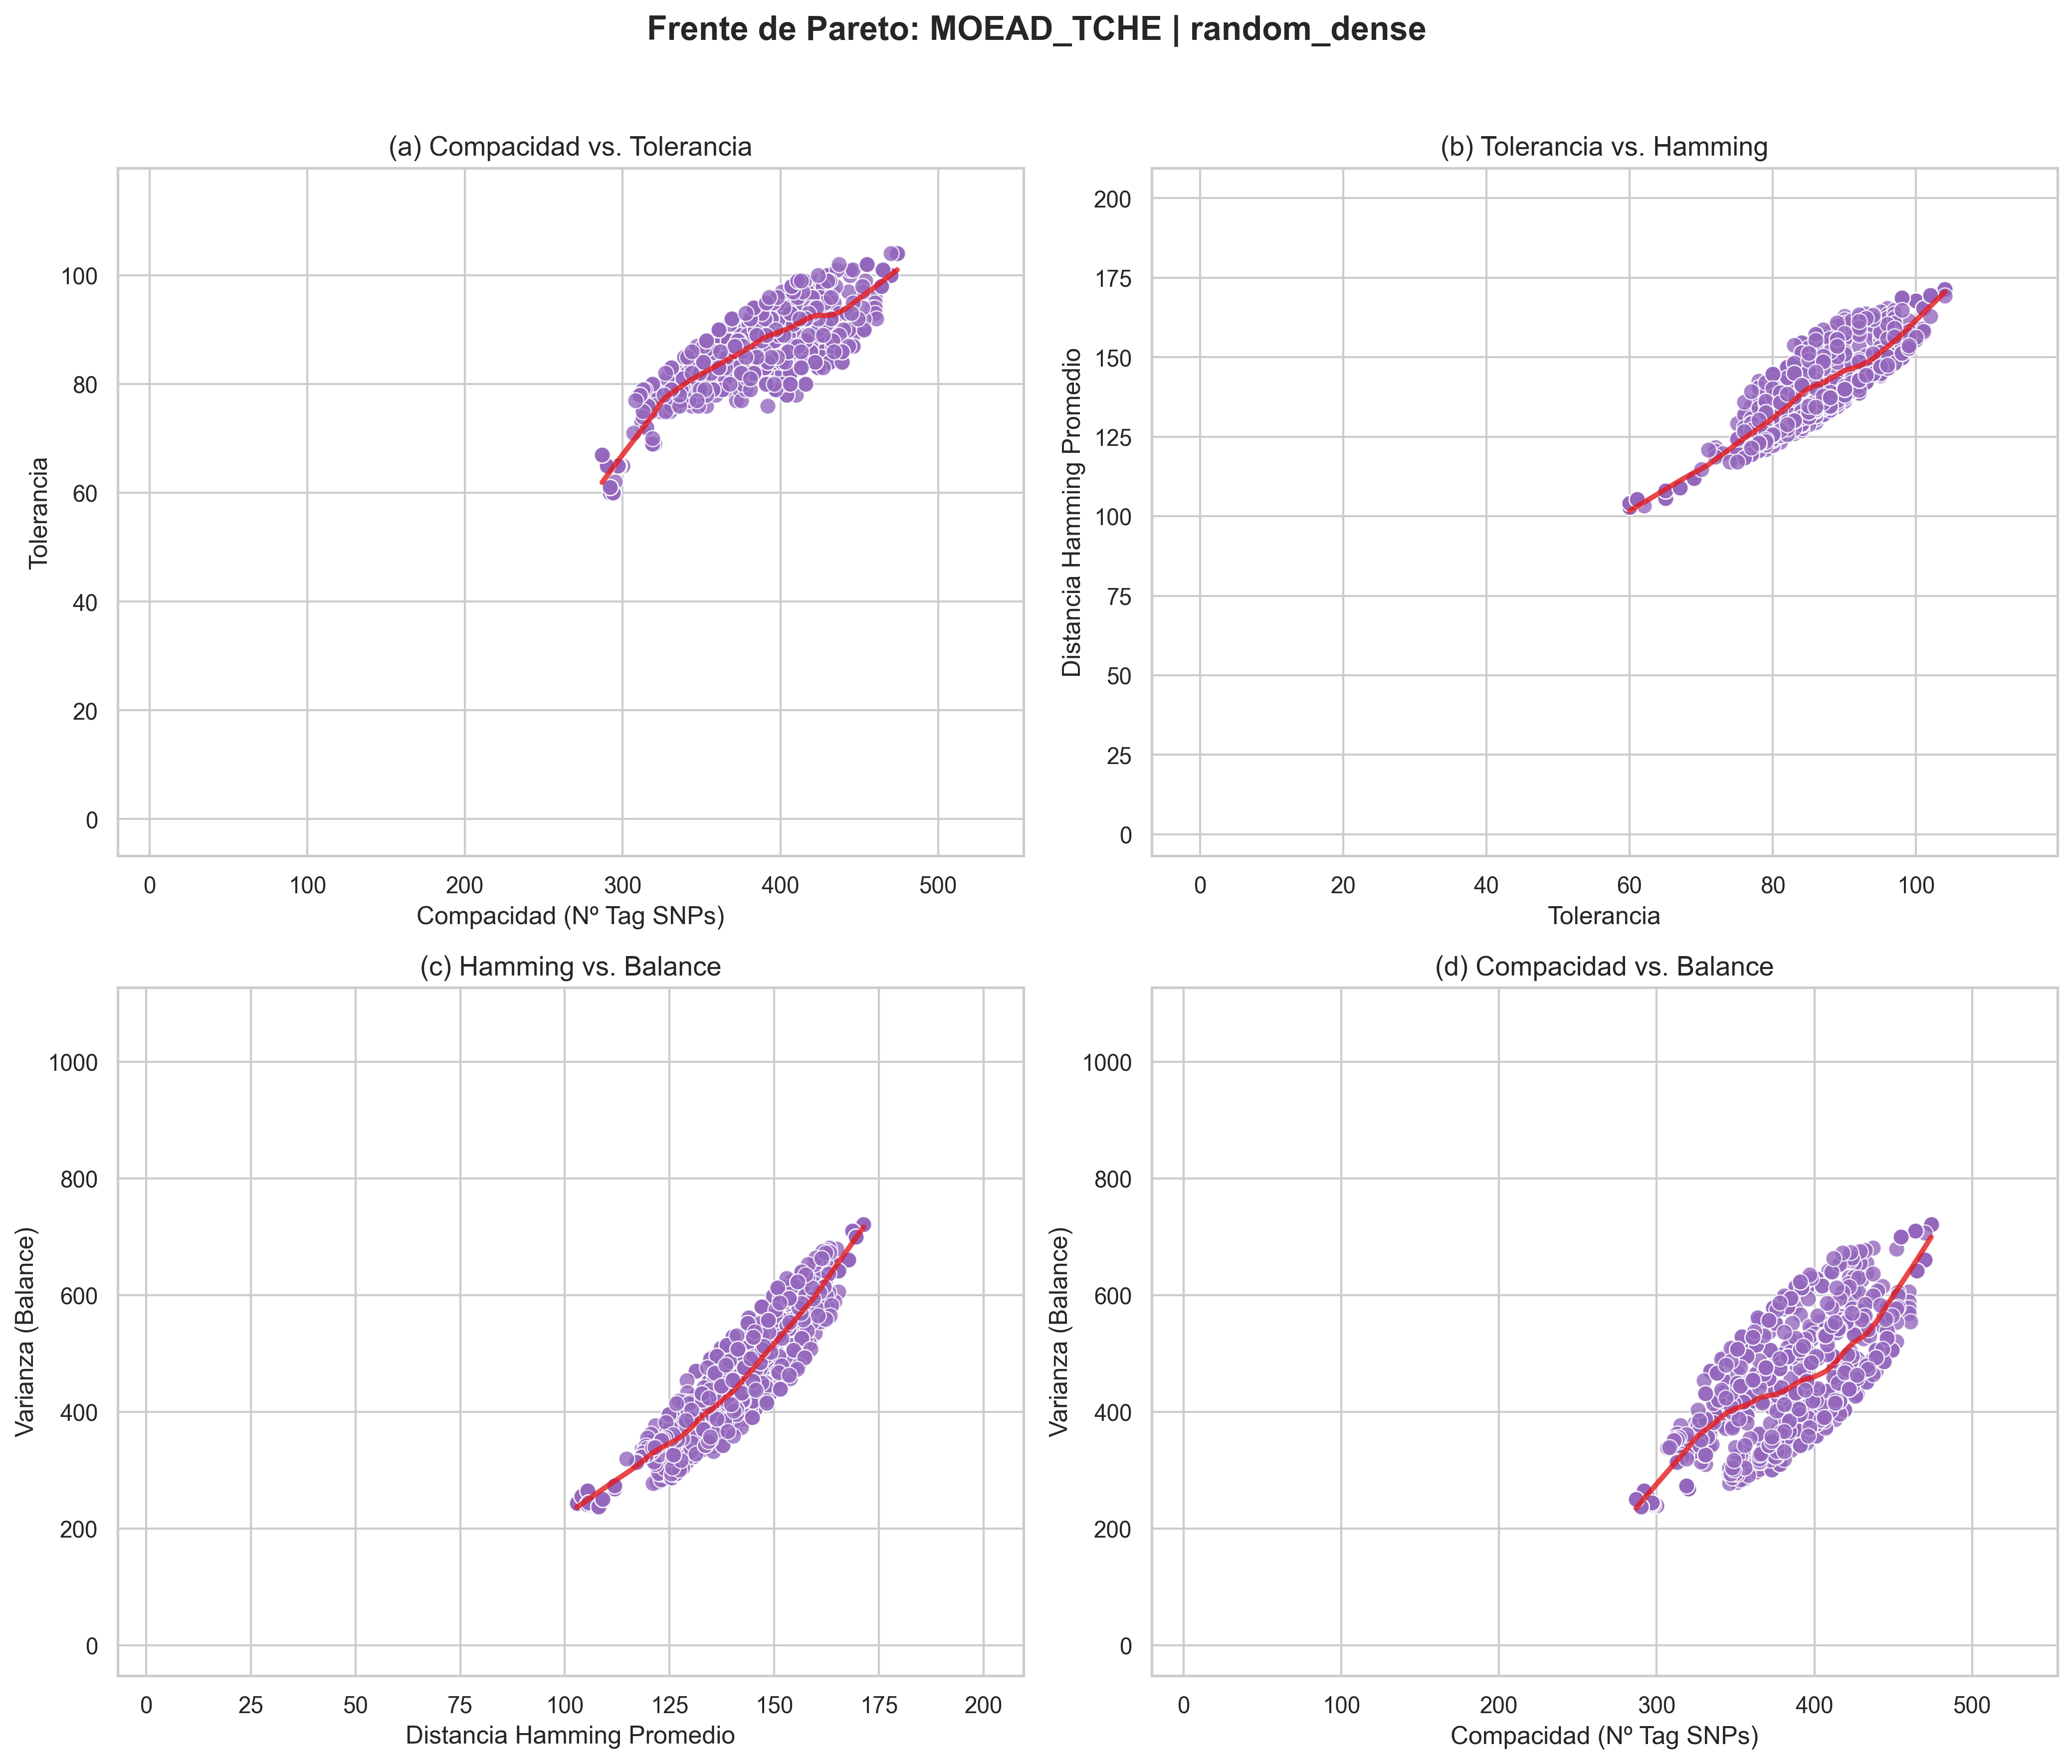
\includegraphics[width=\linewidth]{analisis_assets/20260420T205406/2_comparativa/1_frentes/frentes_pareto/frentes_pareto_moead_tche_random_dense_full.png} & 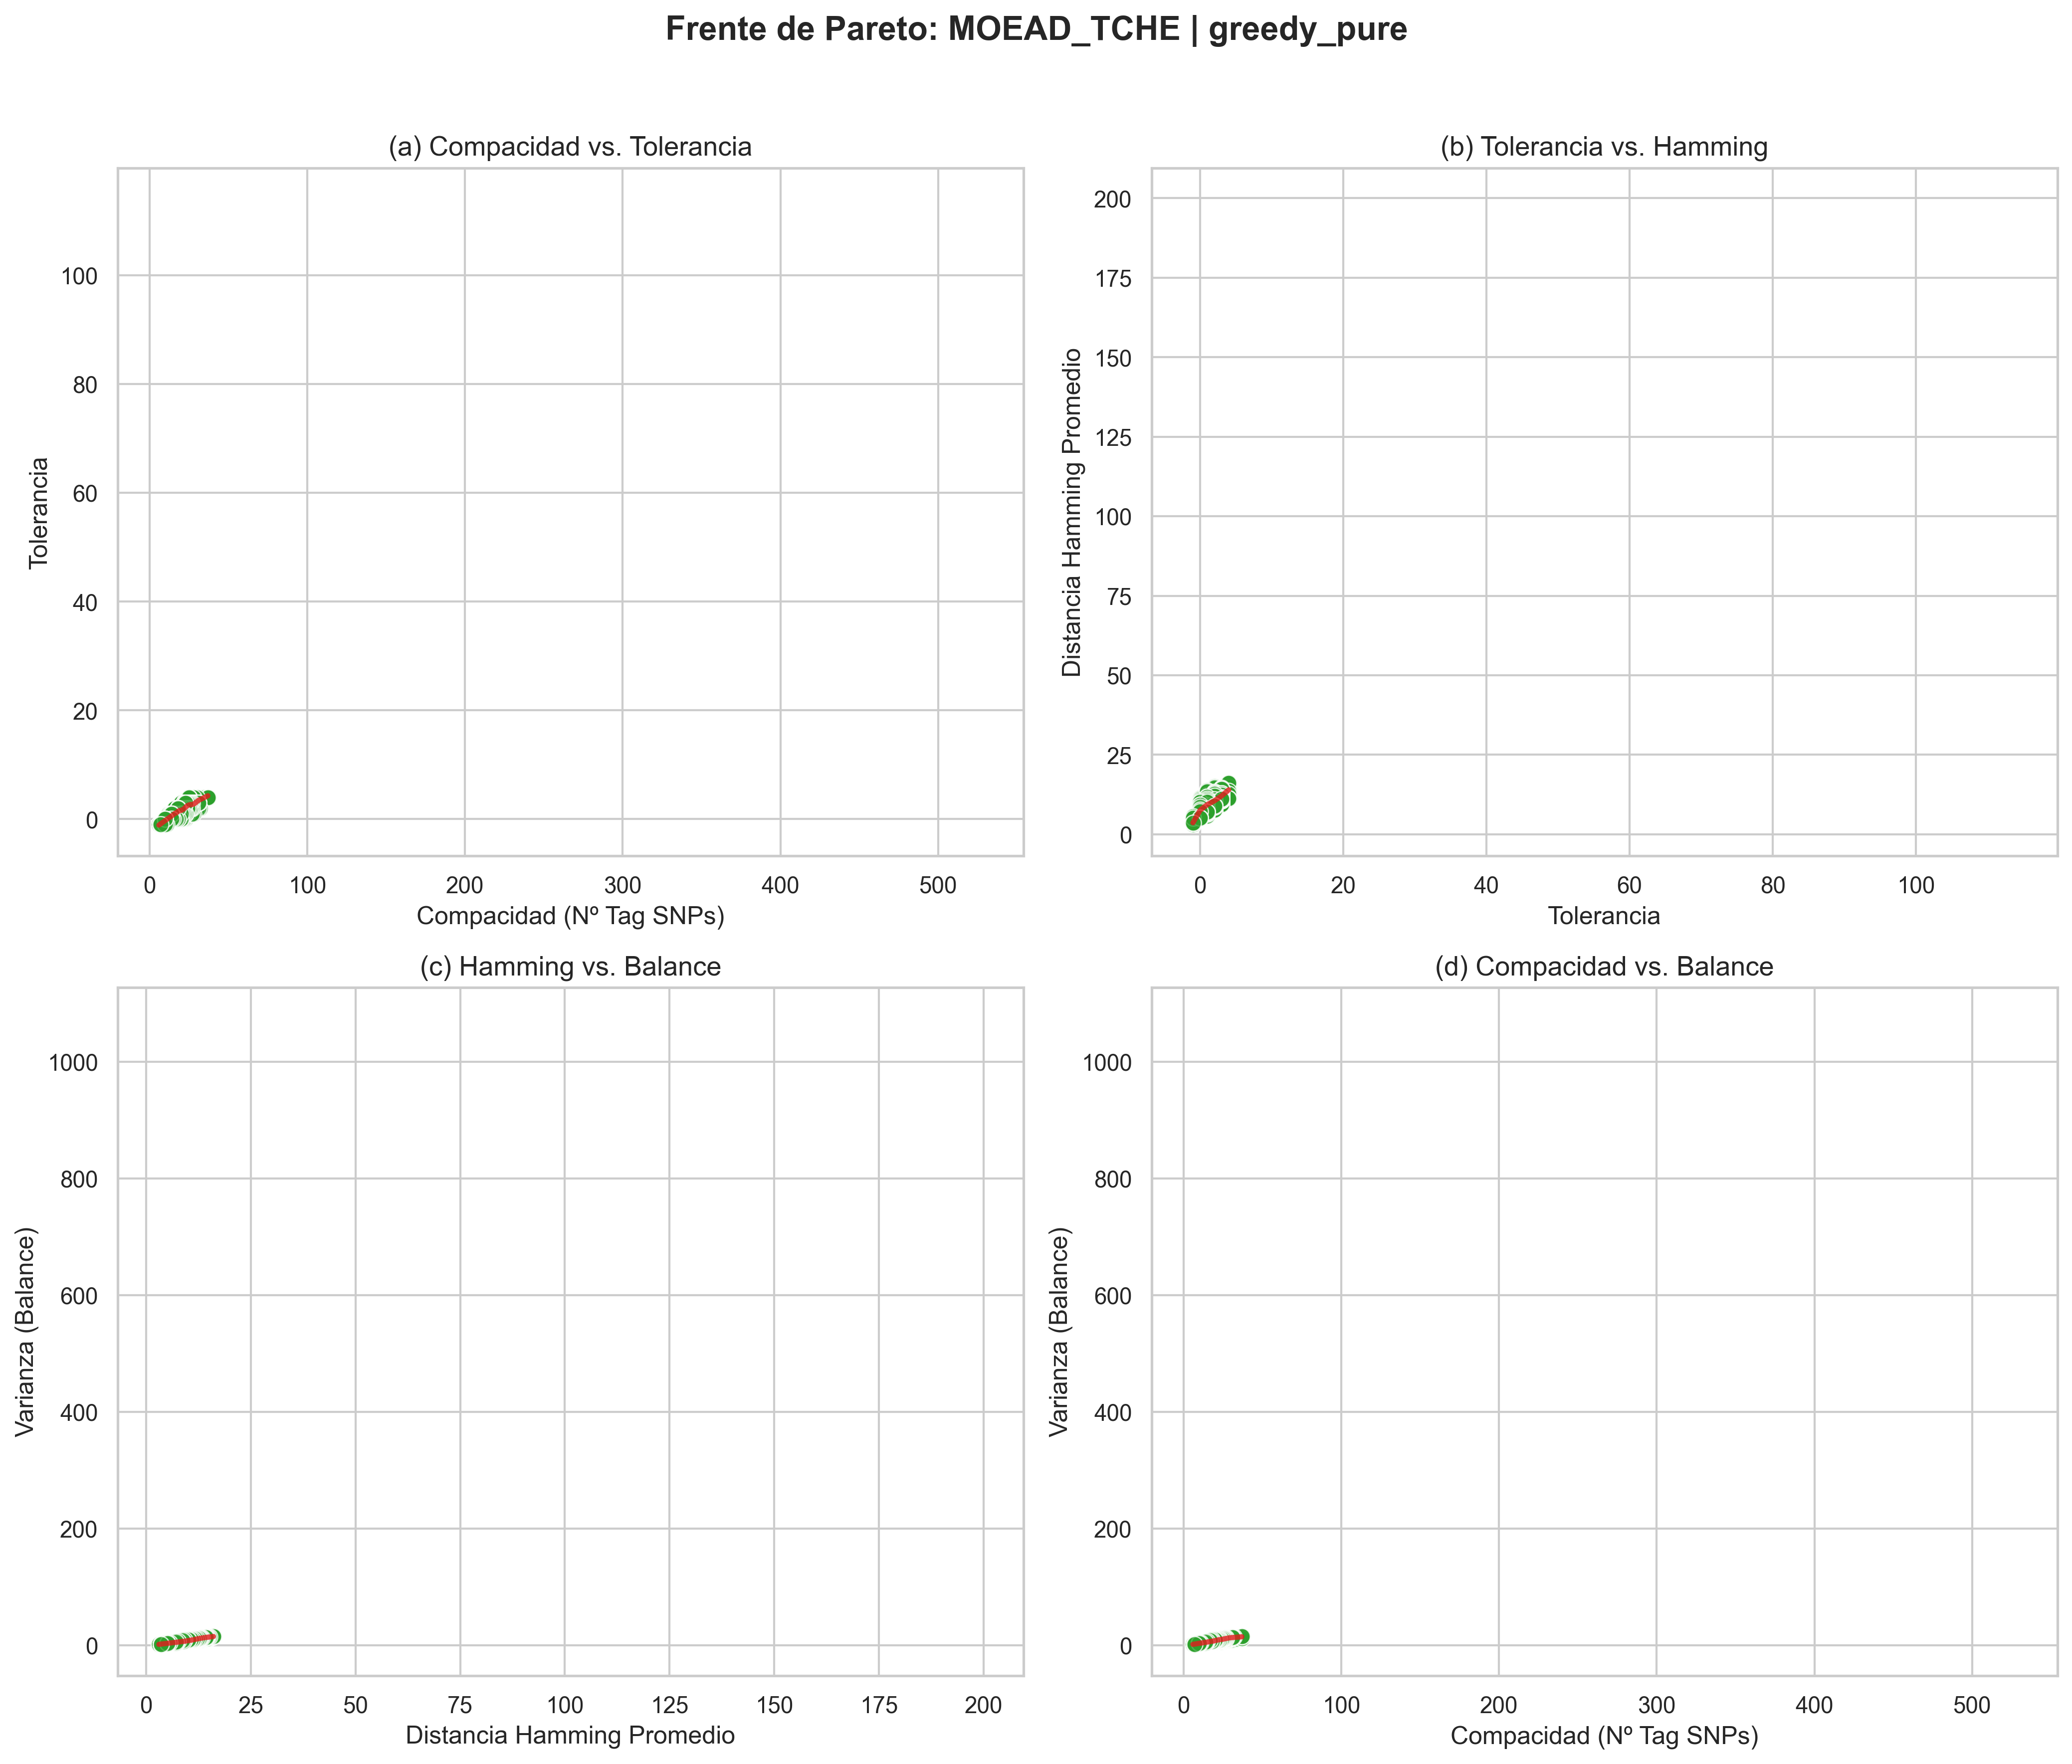
\includegraphics[width=\linewidth]{analisis_assets/20260420T205406/2_comparativa/1_frentes/frentes_pareto/frentes_pareto_moead_tche_greedy_pure_full.png} & 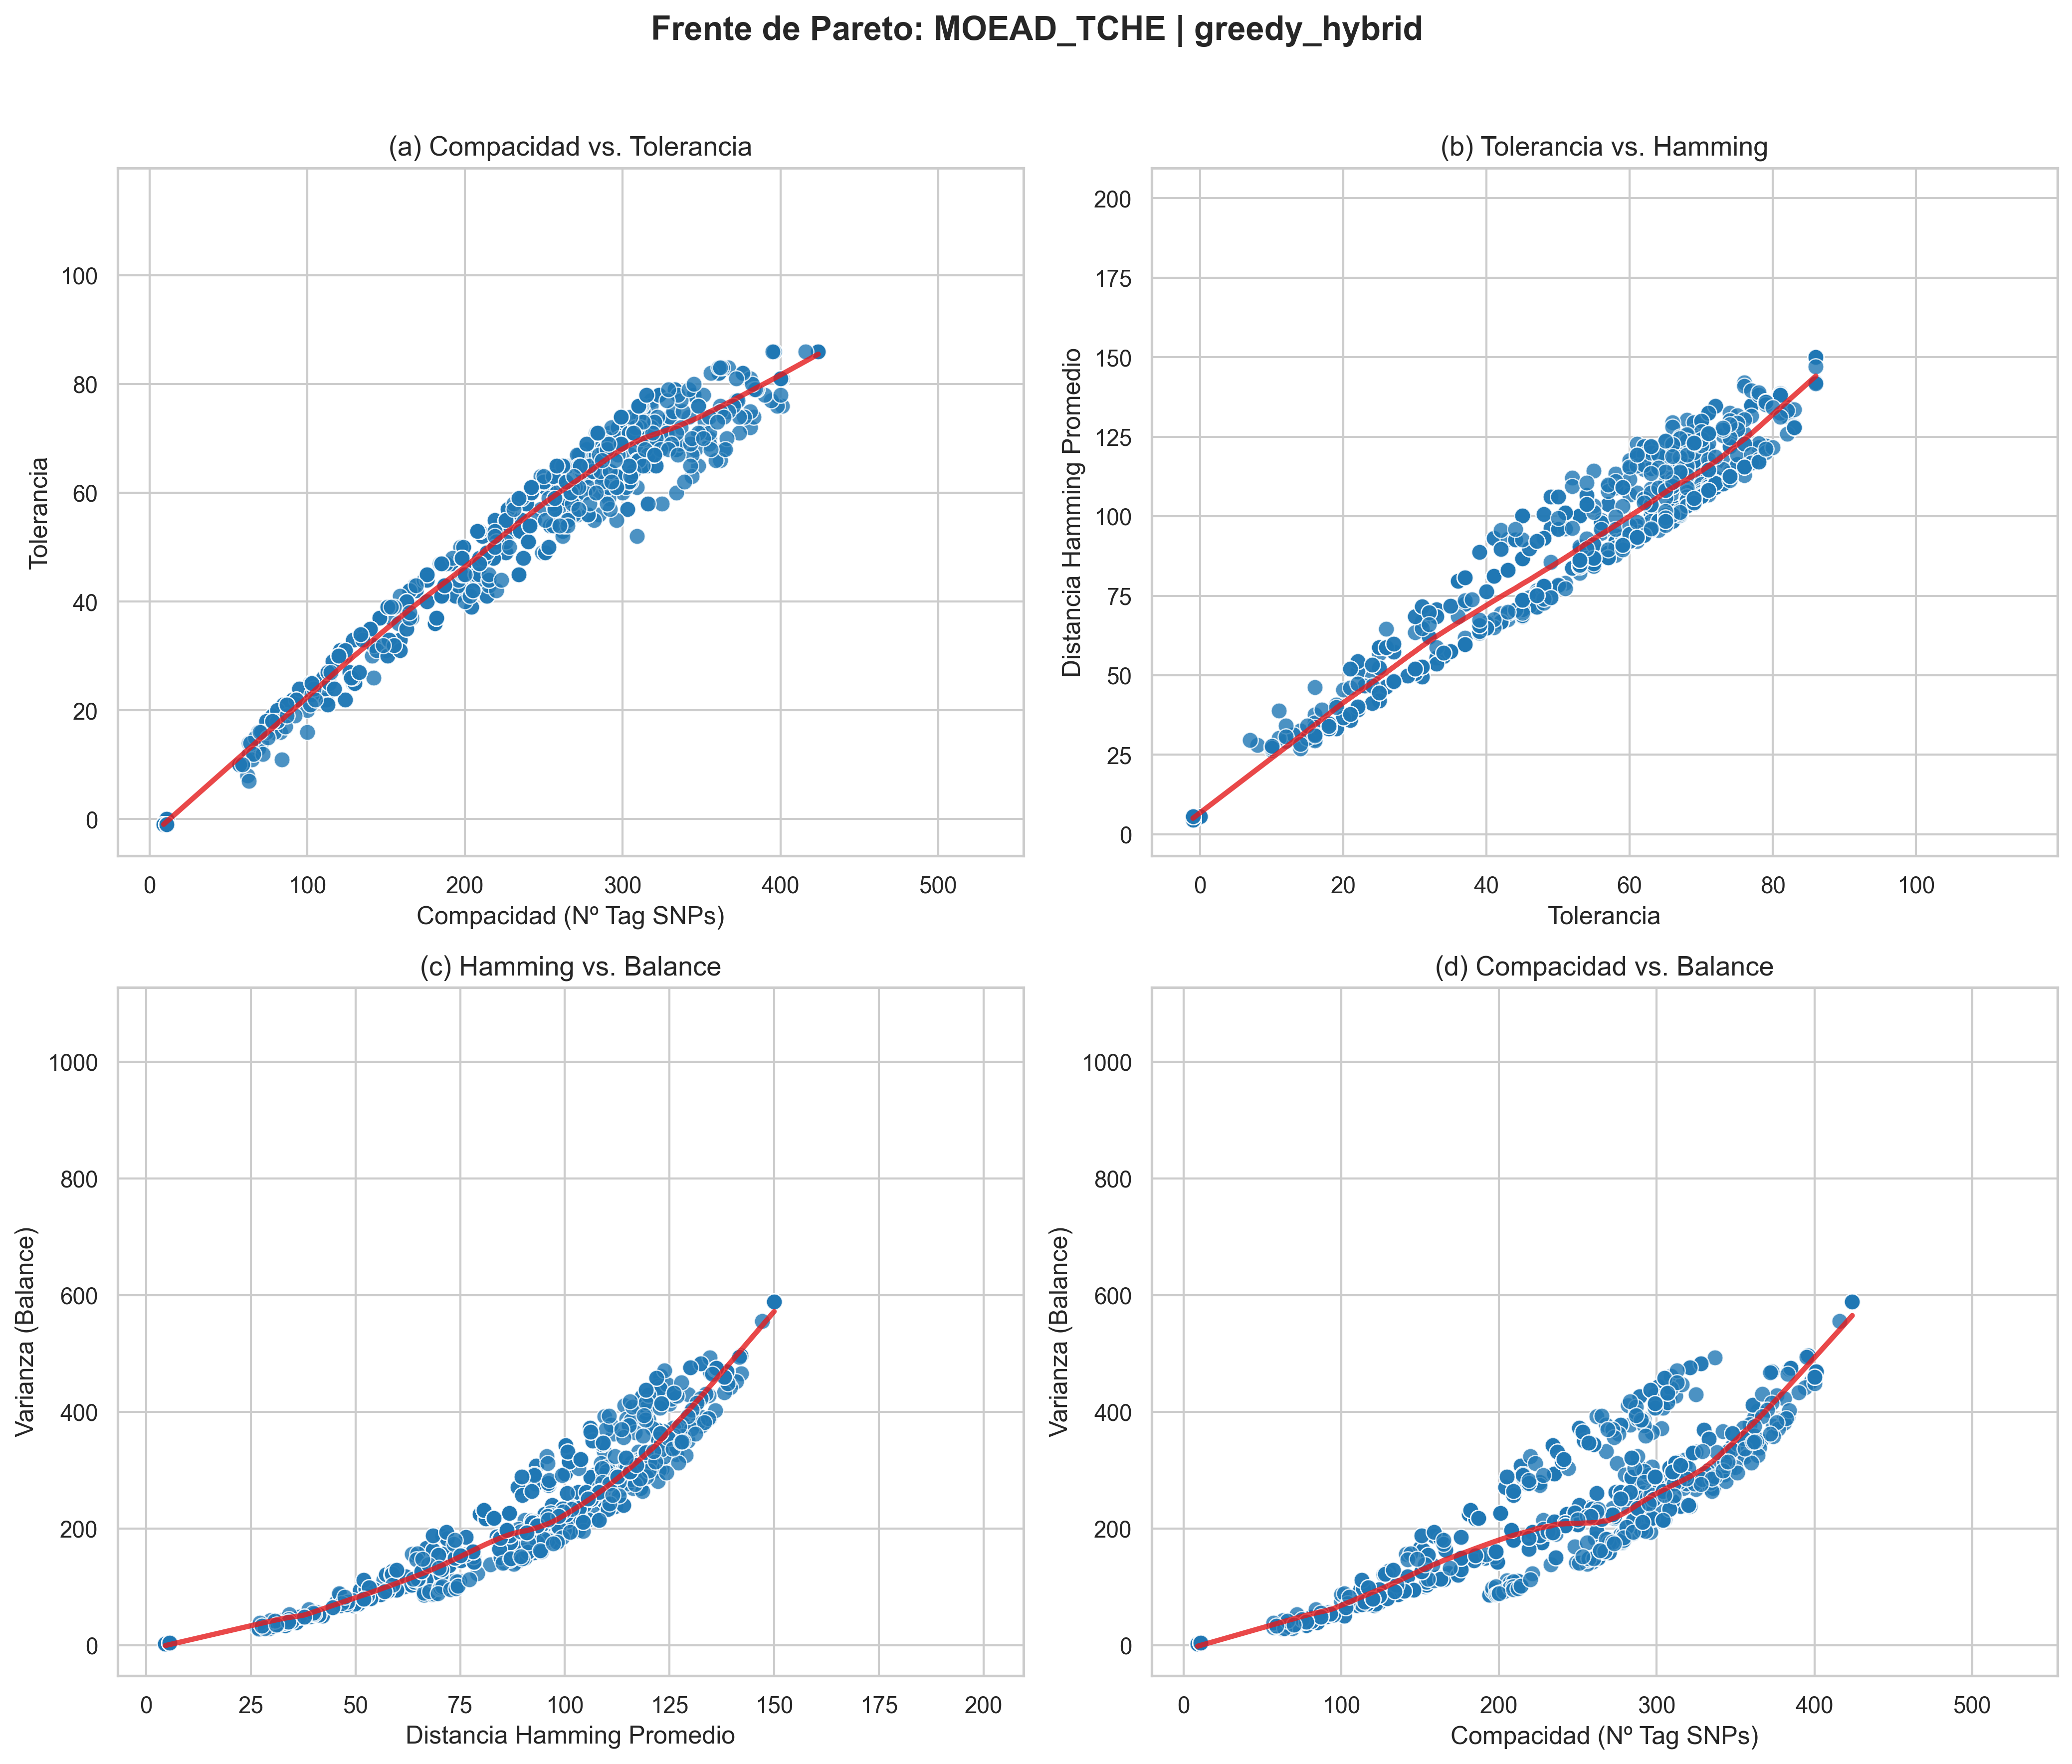
\includegraphics[width=\linewidth]{analisis_assets/20260420T205406/2_comparativa/1_frentes/frentes_pareto/frentes_pareto_moead_tche_greedy_hybrid_full.png} \\
        \textbf{MOEA/D (WS)} & 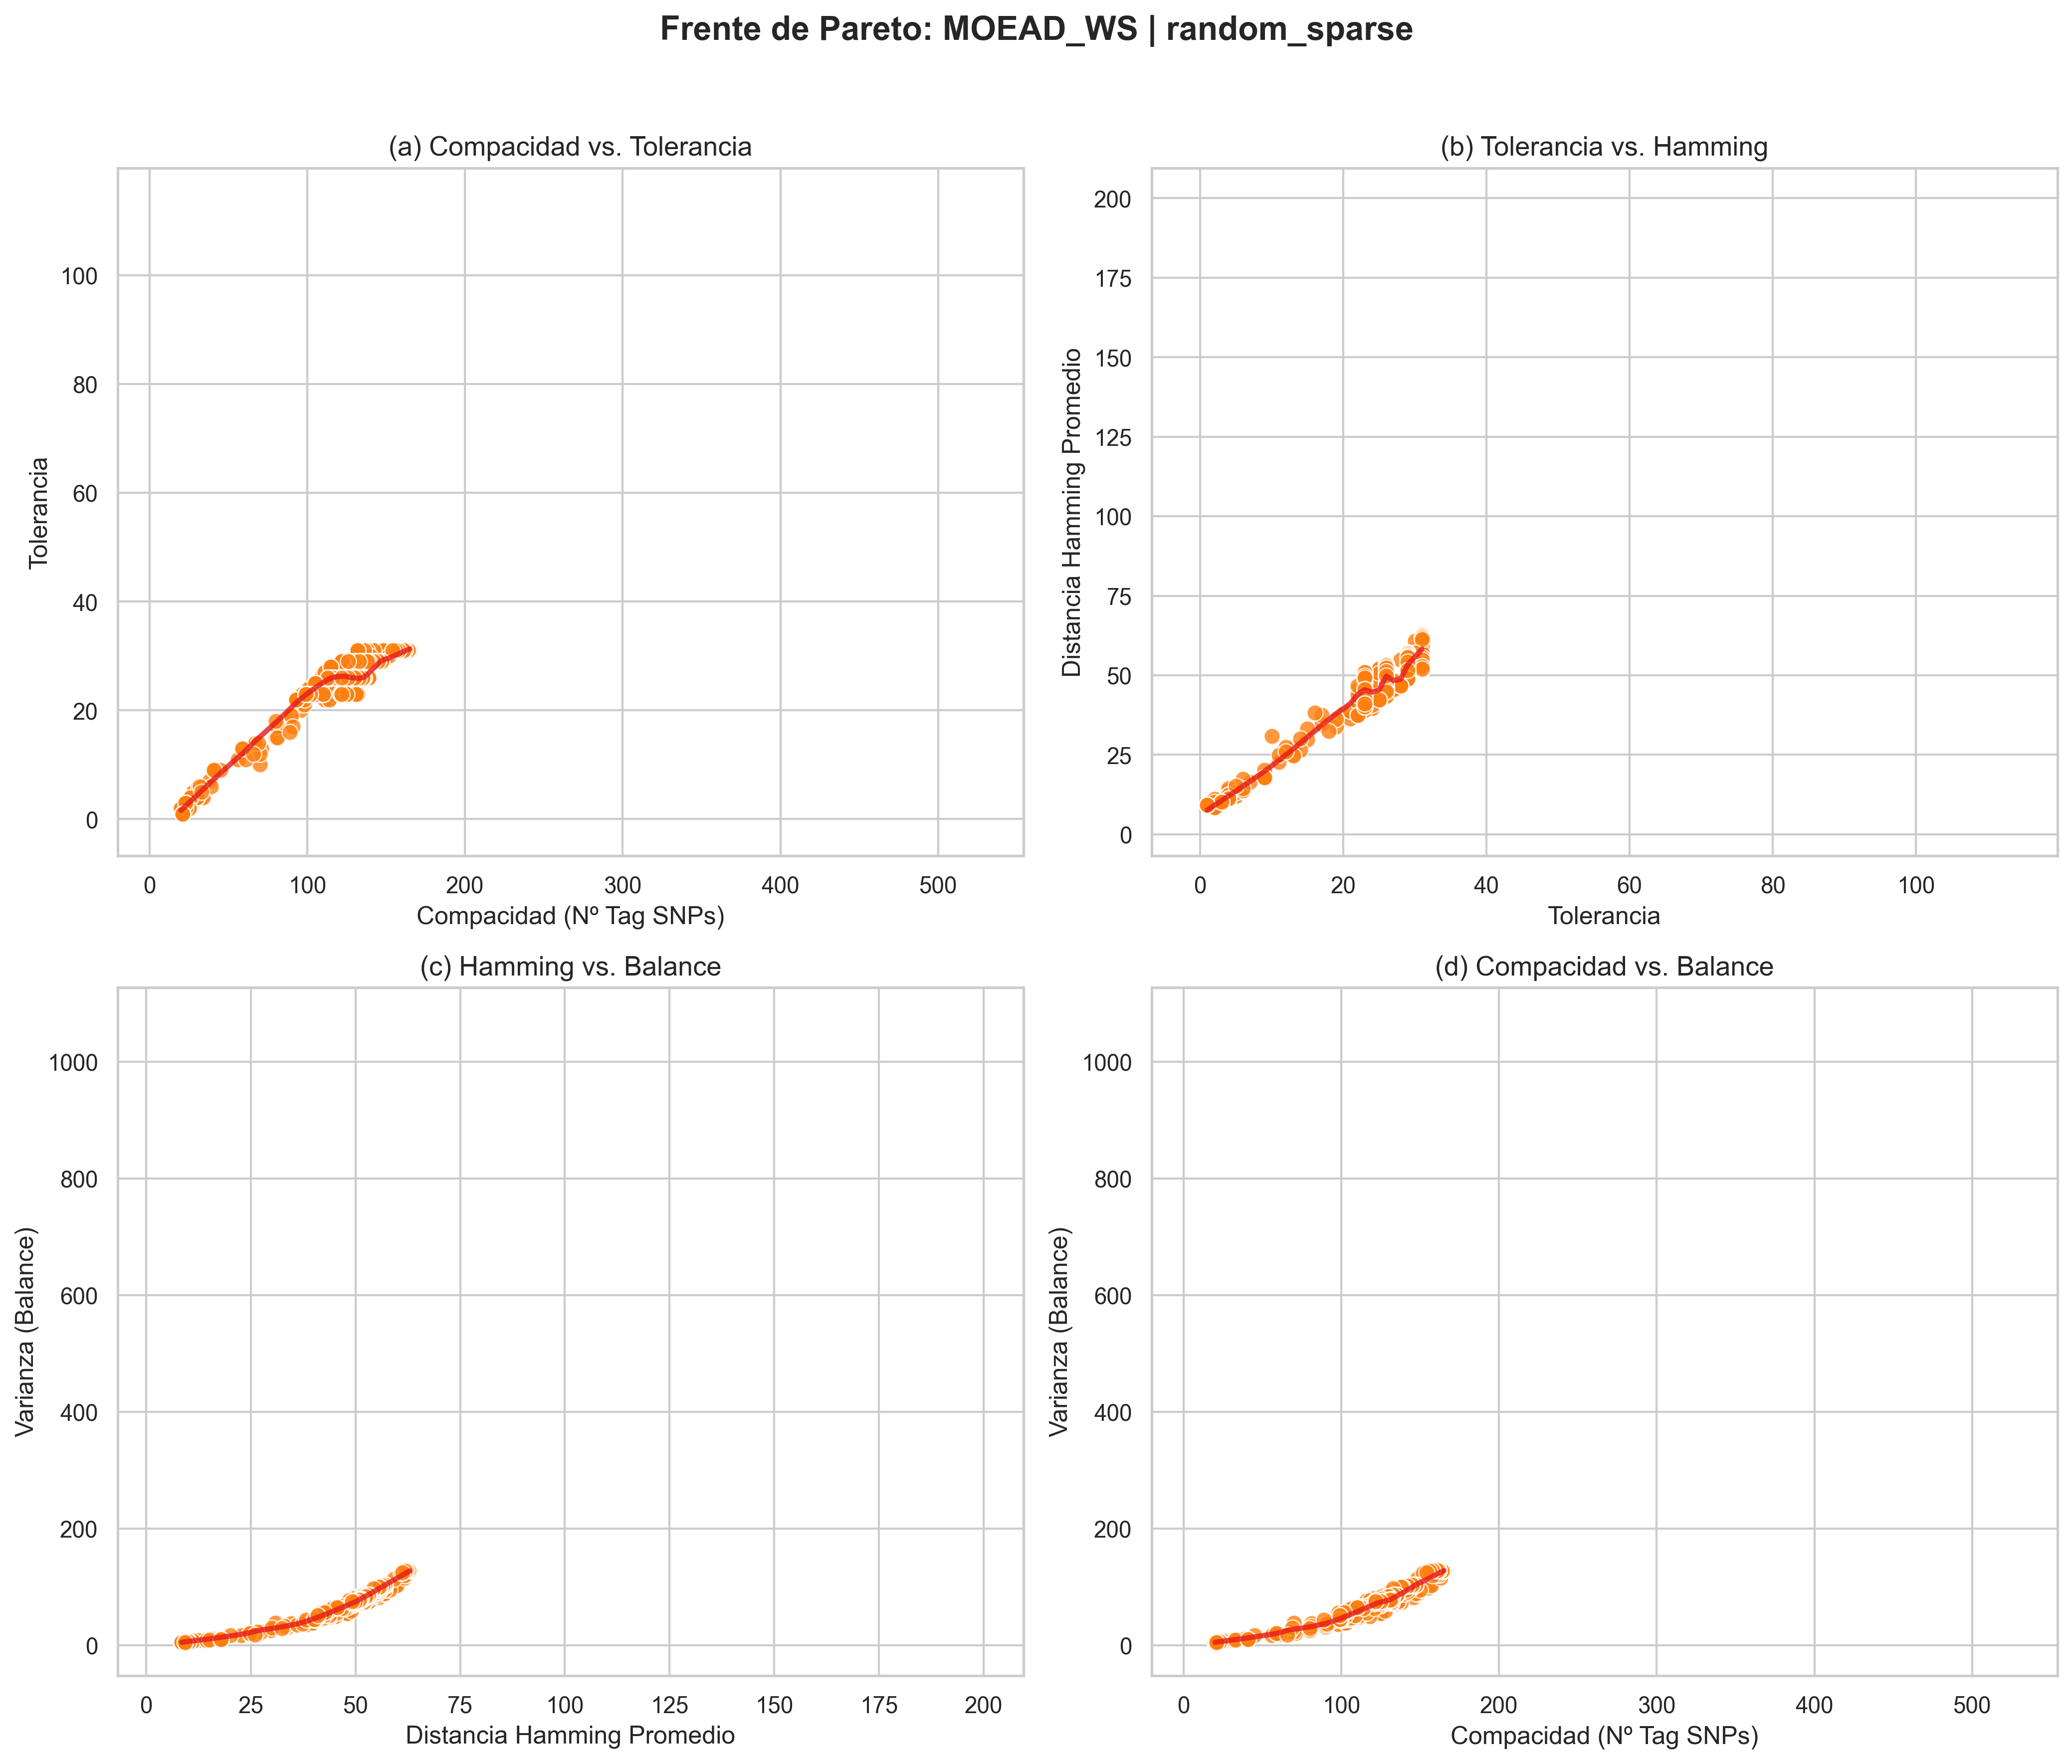
\includegraphics[width=\linewidth]{analisis_assets/20260420T205406/2_comparativa/1_frentes/frentes_pareto/frentes_pareto_moead_ws_random_sparse_full.png} & 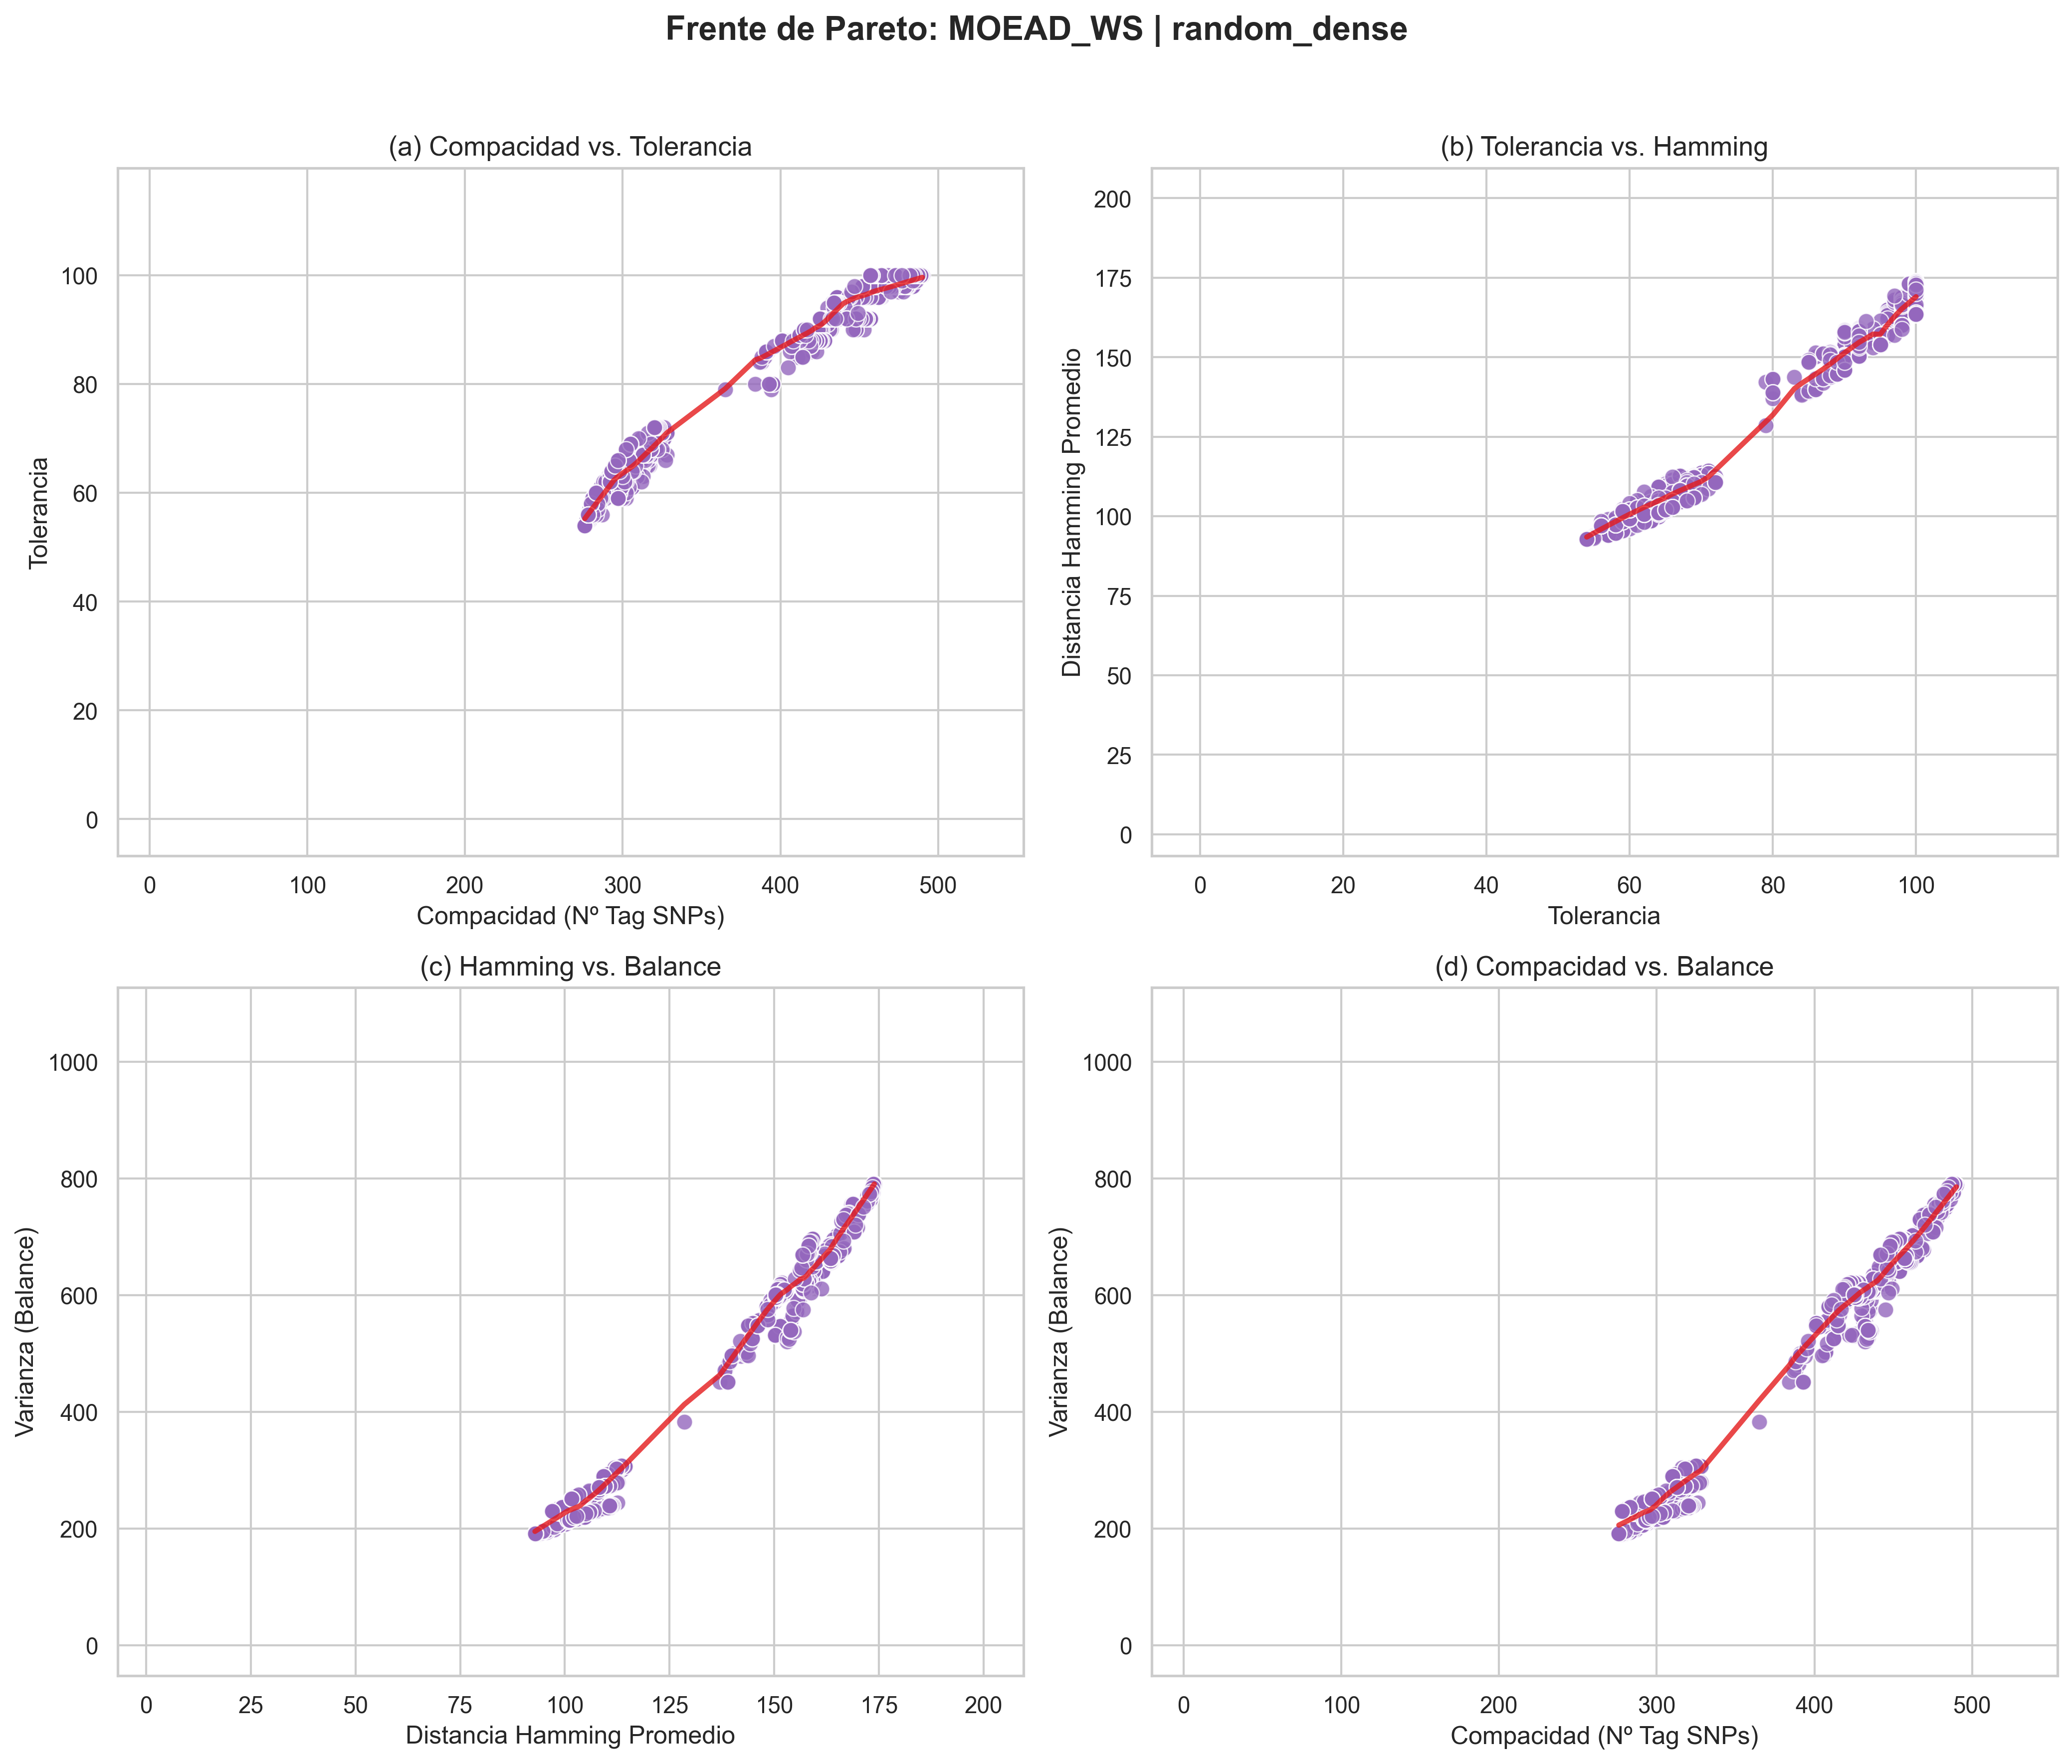
\includegraphics[width=\linewidth]{analisis_assets/20260420T205406/2_comparativa/1_frentes/frentes_pareto/frentes_pareto_moead_ws_random_dense_full.png} & 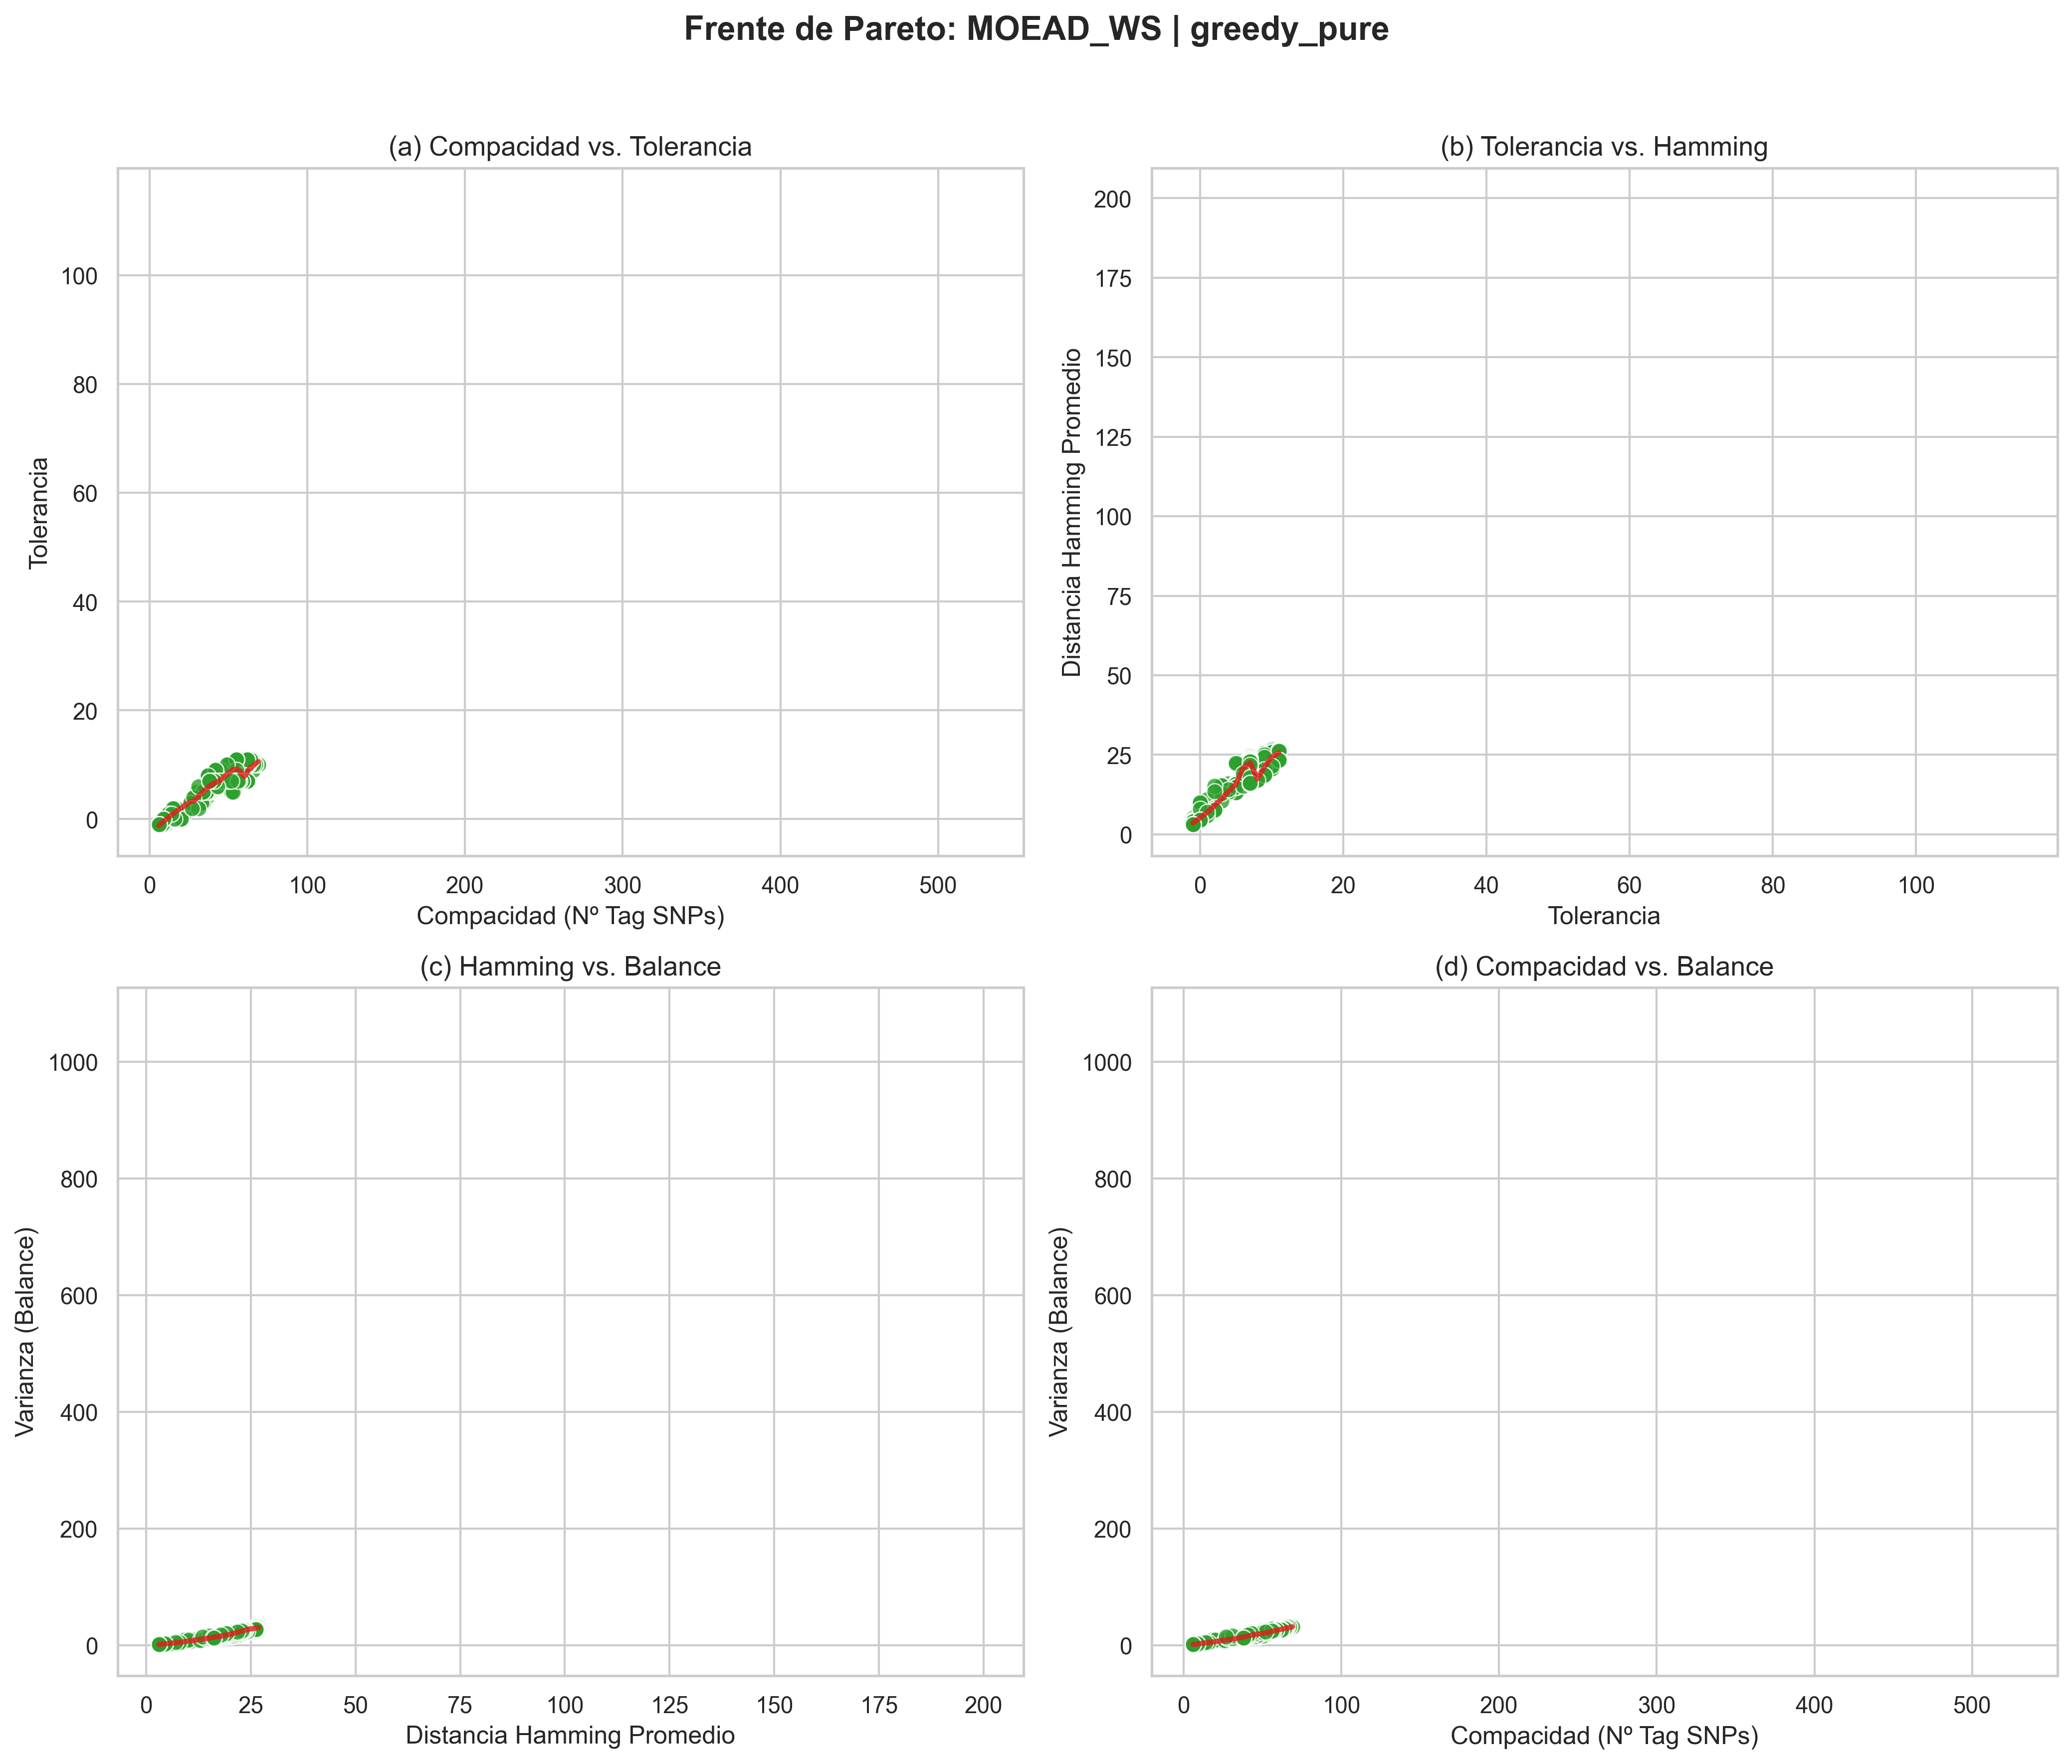
\includegraphics[width=\linewidth]{analisis_assets/20260420T205406/2_comparativa/1_frentes/frentes_pareto/frentes_pareto_moead_ws_greedy_pure_full.png} & 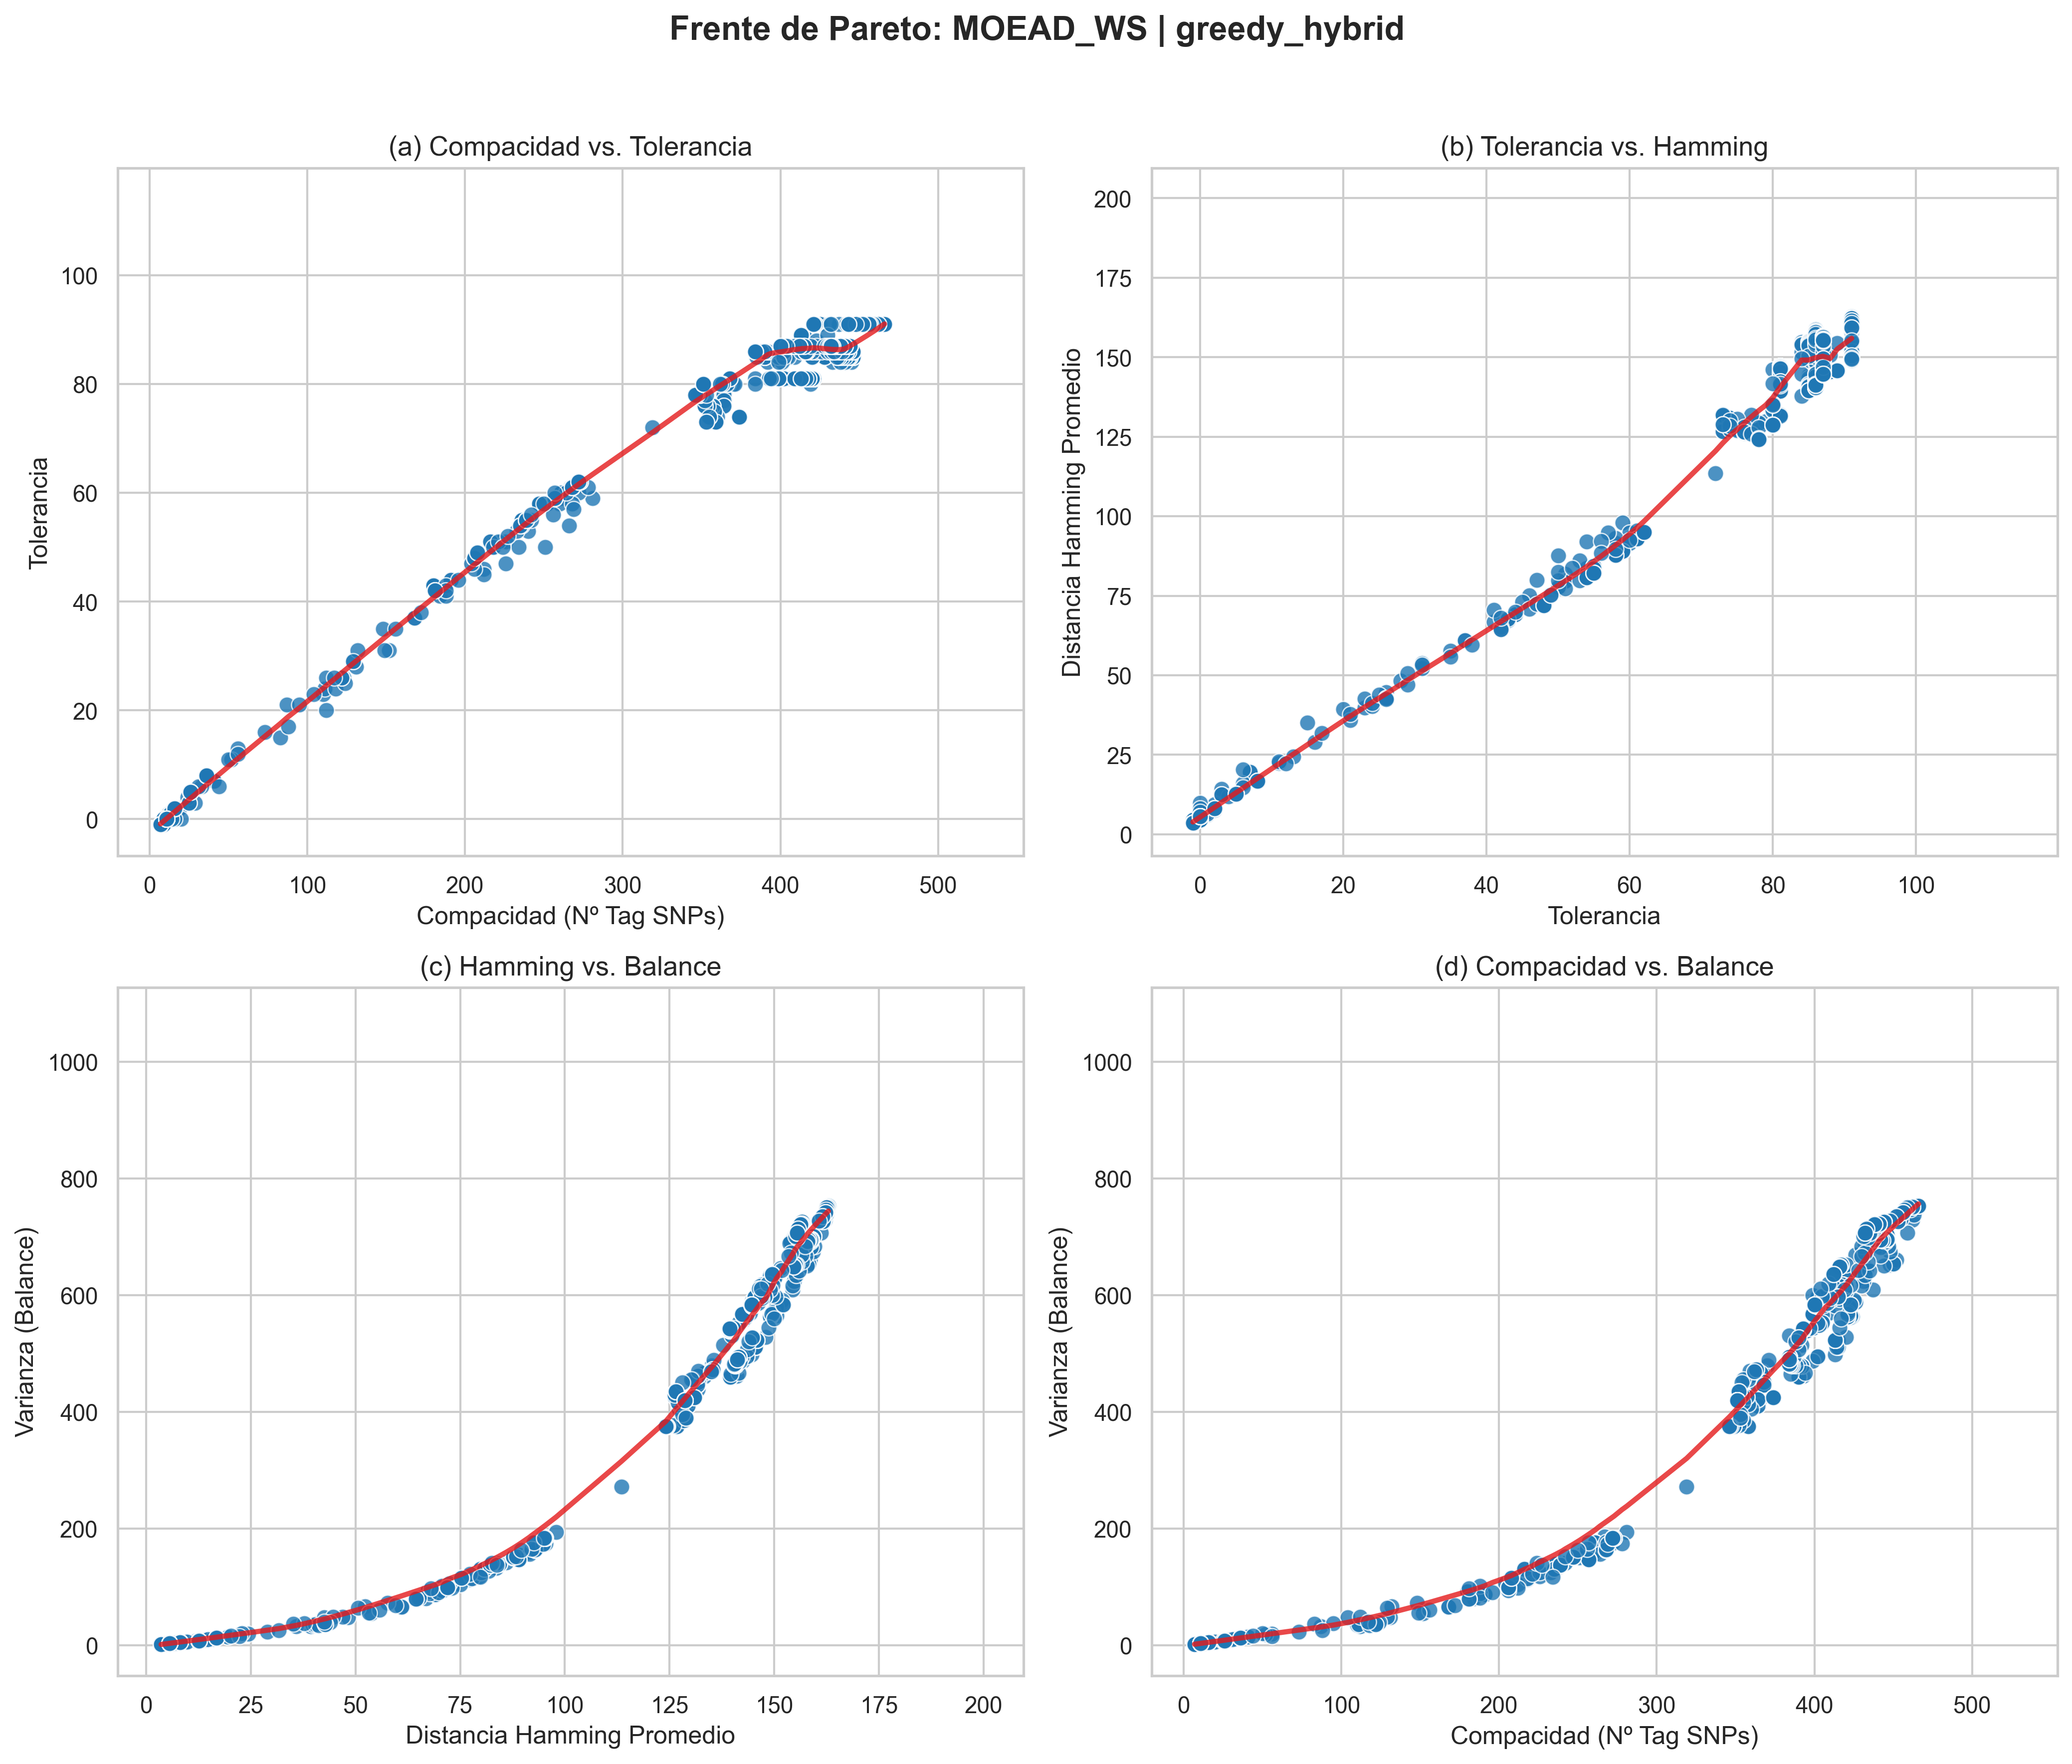
\includegraphics[width=\linewidth]{analisis_assets/20260420T205406/2_comparativa/1_frentes/frentes_pareto/frentes_pareto_moead_ws_greedy_hybrid_full.png} \\
        \bottomrule
    \end{tabular}
    \caption{Galería de Frentes de Pareto (A)}
\end{table}

\paragraph{Convergencia Progresiva (A)}
\begin{figure}[H]
    \centering
    \begin{subfigure}[b]{0.40\textwidth}
        
\includegraphics[width=\textwidth]{analisis_assets/20260420T205406/2_comparativa/2_metricas_convergencia/convergencia_range_full.png}
        \caption{Range}
    \end{subfigure}
    \hfill
    \begin{subfigure}[b]{0.40\textwidth}
        
\includegraphics[width=\textwidth]{analisis_assets/20260420T205406/2_comparativa/2_metricas_convergencia/convergencia_summin_full.png}
        \caption{SumMin}
    \end{subfigure}

    \vspace{0.3cm}

    \begin{subfigure}[b]{0.40\textwidth}
        
\includegraphics[width=\textwidth]{analisis_assets/20260420T205406/2_comparativa/2_metricas_convergencia/convergencia_minsum_full.png}
        \caption{MinSum}
    \end{subfigure}
    \hfill
    \begin{subfigure}[b]{0.40\textwidth}
        
\includegraphics[width=\textwidth]{analisis_assets/20260420T205406/2_comparativa/2_metricas_convergencia/convergencia_maxtolerancerate_full.png}
        \caption{Max. Tolerance Rate}
    \end{subfigure}

    \vspace{0.3cm}

    \begin{subfigure}[b]{0.40\textwidth}
        
\includegraphics[width=\textwidth]{analisis_assets/20260420T205406/2_comparativa/2_metricas_convergencia/convergencia_avgtolerancerate_full.png}
        \caption{Avg. Tolerance Rate}
    \end{subfigure}
    \hfill
    \begin{subfigure}[b]{0.40\textwidth}
        
\includegraphics[width=\textwidth]{analisis_assets/20260420T205406/2_comparativa/2_metricas_convergencia/convergencia_avghammingdistance_full.png}
        \caption{Avg Hamming}
    \end{subfigure}

    \vspace{0.3cm}

    \begin{subfigure}[b]{0.40\textwidth}
        
\includegraphics[width=\textwidth]{analisis_assets/20260420T205406/2_comparativa/2_metricas_convergencia/convergencia_hypervolume_full.png}
        \caption{Hypervolume}
    \end{subfigure}
    \caption{Galería de Convergencia (Ejecución A)}
\end{figure}

\paragraph{Top 10 por Métrica (A)}

\begin{table}[H]
    \centering
    \begin{subtable}[t]{0.45\textwidth}
        \centering
        \caption{Range ($\uparrow$)}
        \begin{tabular}{lllc}
            \toprule
            Pos & Algo & Init & Valor \\
            \midrule
            1 & NSGA2 & GH & 2.4224 \\
            2 & NSGA3 & GH & 1.9282 \\
            3 & SPEA2 & GH & 1.7074 \\
            4 & NSGA2 & RD & 1.9001 \\
            5 & NSGA3 & RD & 1.1689 \\
            6 & SPEA2 & RD & 1.1784 \\
            7 & MOEAD\_TCHE & GH & 1.9002 \\
            8 & MOEAD\_WS & GH & 2.1539 \\
            9 & MOEAD\_TCHE & RD & 0.9234 \\
            10 & MOEAD\_WS & RD & 0.9899 \\
            \bottomrule
        \end{tabular}
    \end{subtable}
    \hfill
    \begin{subtable}[t]{0.45\textwidth}
        \centering
        \caption{SumMin ($\downarrow$)}
        \begin{tabular}{lllc}
            \toprule
            Pos & Algo & Init & Valor \\
            \midrule
            1 & NSGA2 & GH & 0.5507 \\
            2 & NSGA2 & RD & 0.6629 \\
            3 & MOEAD\_WS & GH & 0.7268 \\
            4 & NSGA3 & GH & 0.8041 \\
            5 & MOEAD\_TCHE & GH & 0.8226 \\
            6 & NSGA3 & RD & 0.9285 \\
            7 & SPEA2 & GH & 0.9367 \\
            8 & MOEAD\_PBI & GH & 0.9422 \\
            9 & SPEA2 & RD & 1.0520 \\
            10 & MOEAD\_TCHE & RD & 1.0648 \\
            \bottomrule
        \end{tabular}
    \end{subtable}
\end{table}

\begin{table}[H]
    \centering
    \begin{subtable}[t]{0.45\textwidth}
        \centering
        \caption{MinSum ($\downarrow$)}
        \begin{tabular}{lllc}
            \toprule
            Pos & Algo & Init & Valor \\
            \midrule
            1 & NSGA3 & RD & 1.4001 \\
            2 & MOEAD\_TCHE & RD & 1.4335 \\
            3 & NSGA2 & RD & 1.4417 \\
            4 & MOEAD\_PBI & RD & 1.4680 \\
            5 & SPEA2 & RD & 1.4752 \\
            6 & NSGA3 & GH & 1.4848 \\
            7 & NSGA2 & GH & 1.4944 \\
            8 & MOEAD\_WS & RD & 1.4961 \\
            9 & MOEAD\_PBI & GH & 1.5042 \\
            10 & MOEAD\_TCHE & GH & 1.5114 \\
            \bottomrule
        \end{tabular}
    \end{subtable}
    \hfill
    \begin{subtable}[t]{0.45\textwidth}
        \centering
        \caption{Max. Tolerance Rate ($\uparrow$)}
        \begin{tabular}{lllc}
            \toprule
            Pos & Algo & Init & Valor \\
            \midrule
            1 & MOEAD\_PBI & GH & 0.2745 \\
            2 & MOEAD\_PBI & RD & 0.2644 \\
            3 & NSGA3 & RS & 0.2699 \\
            4 & NSGA3 & RD & 0.2517 \\
            5 & NSGA3 & GH & 0.2517 \\
            6 & SPEA2 & RS & 0.2489 \\
            7 & MOEAD\_TCHE & RS & 0.2558 \\
            8 & MOEAD\_PBI & RS & 0.2430 \\
            9 & NSGA2 & GH & 0.2378 \\
            10 & SPEA2 & RD & 0.2338 \\
            \bottomrule
        \end{tabular}
    \end{subtable}
\end{table}

\begin{table}[H]
    \centering
    \begin{subtable}[t]{0.45\textwidth}
        \centering
        \caption{Avg. Tolerance Rate ($\uparrow$)}
        \begin{tabular}{lllc}
            \toprule
            Pos & Algo & Init & Valor \\
            \midrule
            1 & MOEAD\_PBI & GH & 0.2362 \\
            2 & MOEAD\_TCHE & RD & 0.2252 \\
            3 & MOEAD\_PBI & RD & 0.2244 \\
            4 & NSGA3 & RS & 0.2220 \\
            5 & MOEAD\_TCHE & RS & 0.2183 \\
            6 & NSGA3 & RD & 0.2164 \\
            7 & NSGA2 & RD & 0.2143 \\
            8 & MOEAD\_PBI & RS & 0.2127 \\
            9 & MOEAD\_WS & RD & 0.2111 \\
            10 & MOEAD\_TCHE & GH & 0.2085 \\
            \bottomrule
        \end{tabular}
    \end{subtable}
    \hfill
    \begin{subtable}[t]{0.45\textwidth}
        \centering
        \caption{Avg. Hamming ($\uparrow$)}
        \begin{tabular}{lllc}
            \toprule
            Pos & Algo & Init & Valor \\
            \midrule
            1 & SPEA2 & RD & 149.59 \\
            2 & NSGA3 & RD & 144.52 \\
            3 & MOEAD\_TCHE & RD & 140.48 \\
            4 & NSGA2 & RD & 139.53 \\
            5 & MOEAD\_PBI & RD & 138.13 \\
            6 & MOEAD\_WS & RD & 135.75 \\
            7 & SPEA2 & GH & 105.36 \\
            8 & NSGA2 & GH & 99.45 \\
            9 & MOEAD\_WS & GH & 97.80 \\
            10 & MOEAD\_PBI & GH & 94.63 \\
            \bottomrule
        \end{tabular}
    \end{subtable}
\end{table}

\begin{table}[H]
    \centering
    \caption{Hypervolume ($\uparrow$)}
    \begin{tabular}{lllc}
        \toprule
        Pos & Algoritmo & Inicialización & Valor \\
        \midrule
        1 & NSGA2 & greedy\_hybrid & 0.2446 \\
        2 & NSGA2 & random\_dense & 0.2367 \\
        3 & MOEAD\_TCHE & greedy\_hybrid & 0.2337 \\
        4 & MOEAD\_PBI & greedy\_hybrid & 0.2214 \\
        5 & NSGA3 & greedy\_hybrid & 0.2173 \\
        6 & NSGA3 & random\_dense & 0.2083 \\
        7 & MOEAD\_WS & greedy\_hybrid & 0.2046 \\
        8 & SPEA2 & greedy\_hybrid & 0.1979 \\
        9 & MOEAD\_TCHE & random\_dense & 0.1891 \\
        10 & SPEA2 & random\_dense & 0.1685 \\
        \bottomrule
    \end{tabular}
\end{table}

\paragraph{Correlación de Métricas (Heatmap)}
\begin{figure}[H]
    \centering
    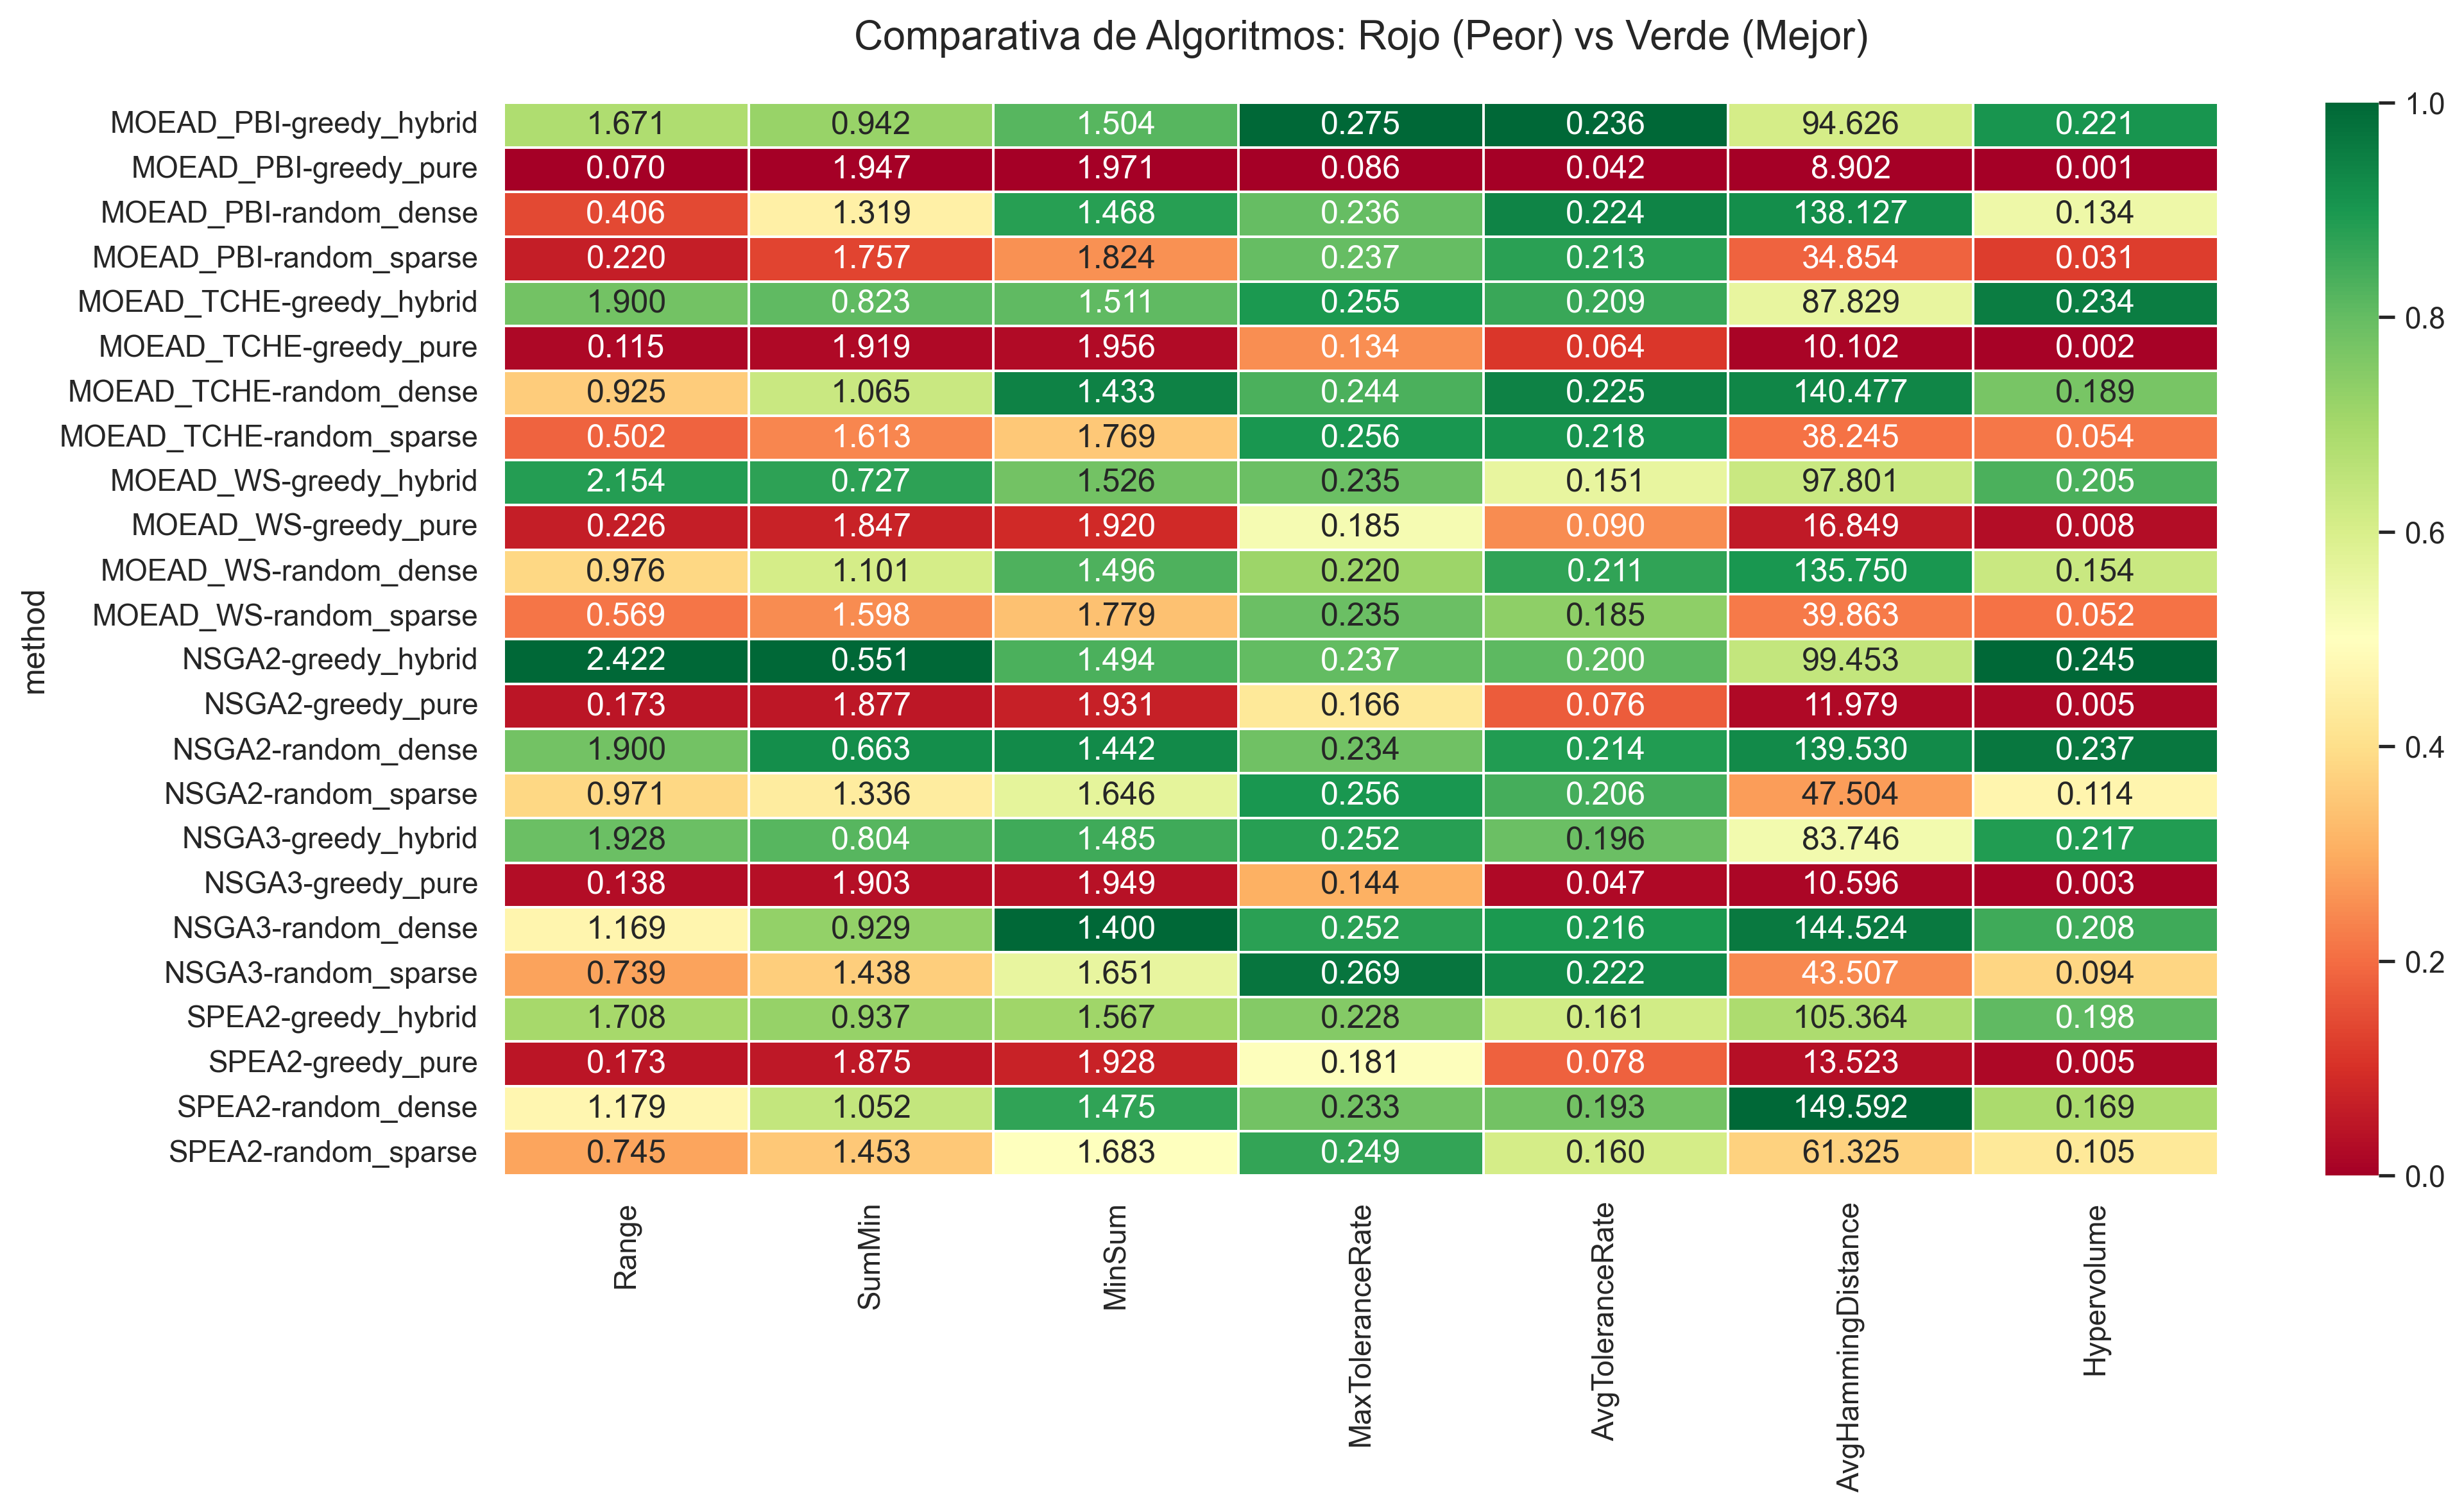
\includegraphics[width=0.6\textwidth]{analisis_assets/20260420T205406/2_comparativa/4_rankings/heatmap_comparativa_full.png}
    \caption{Comparativa de métricas para la Ejecución A.}
\end{figure}

\paragraph{Ranking Global (Rank-Sum)}
\begin{figure}[H]
    \centering
    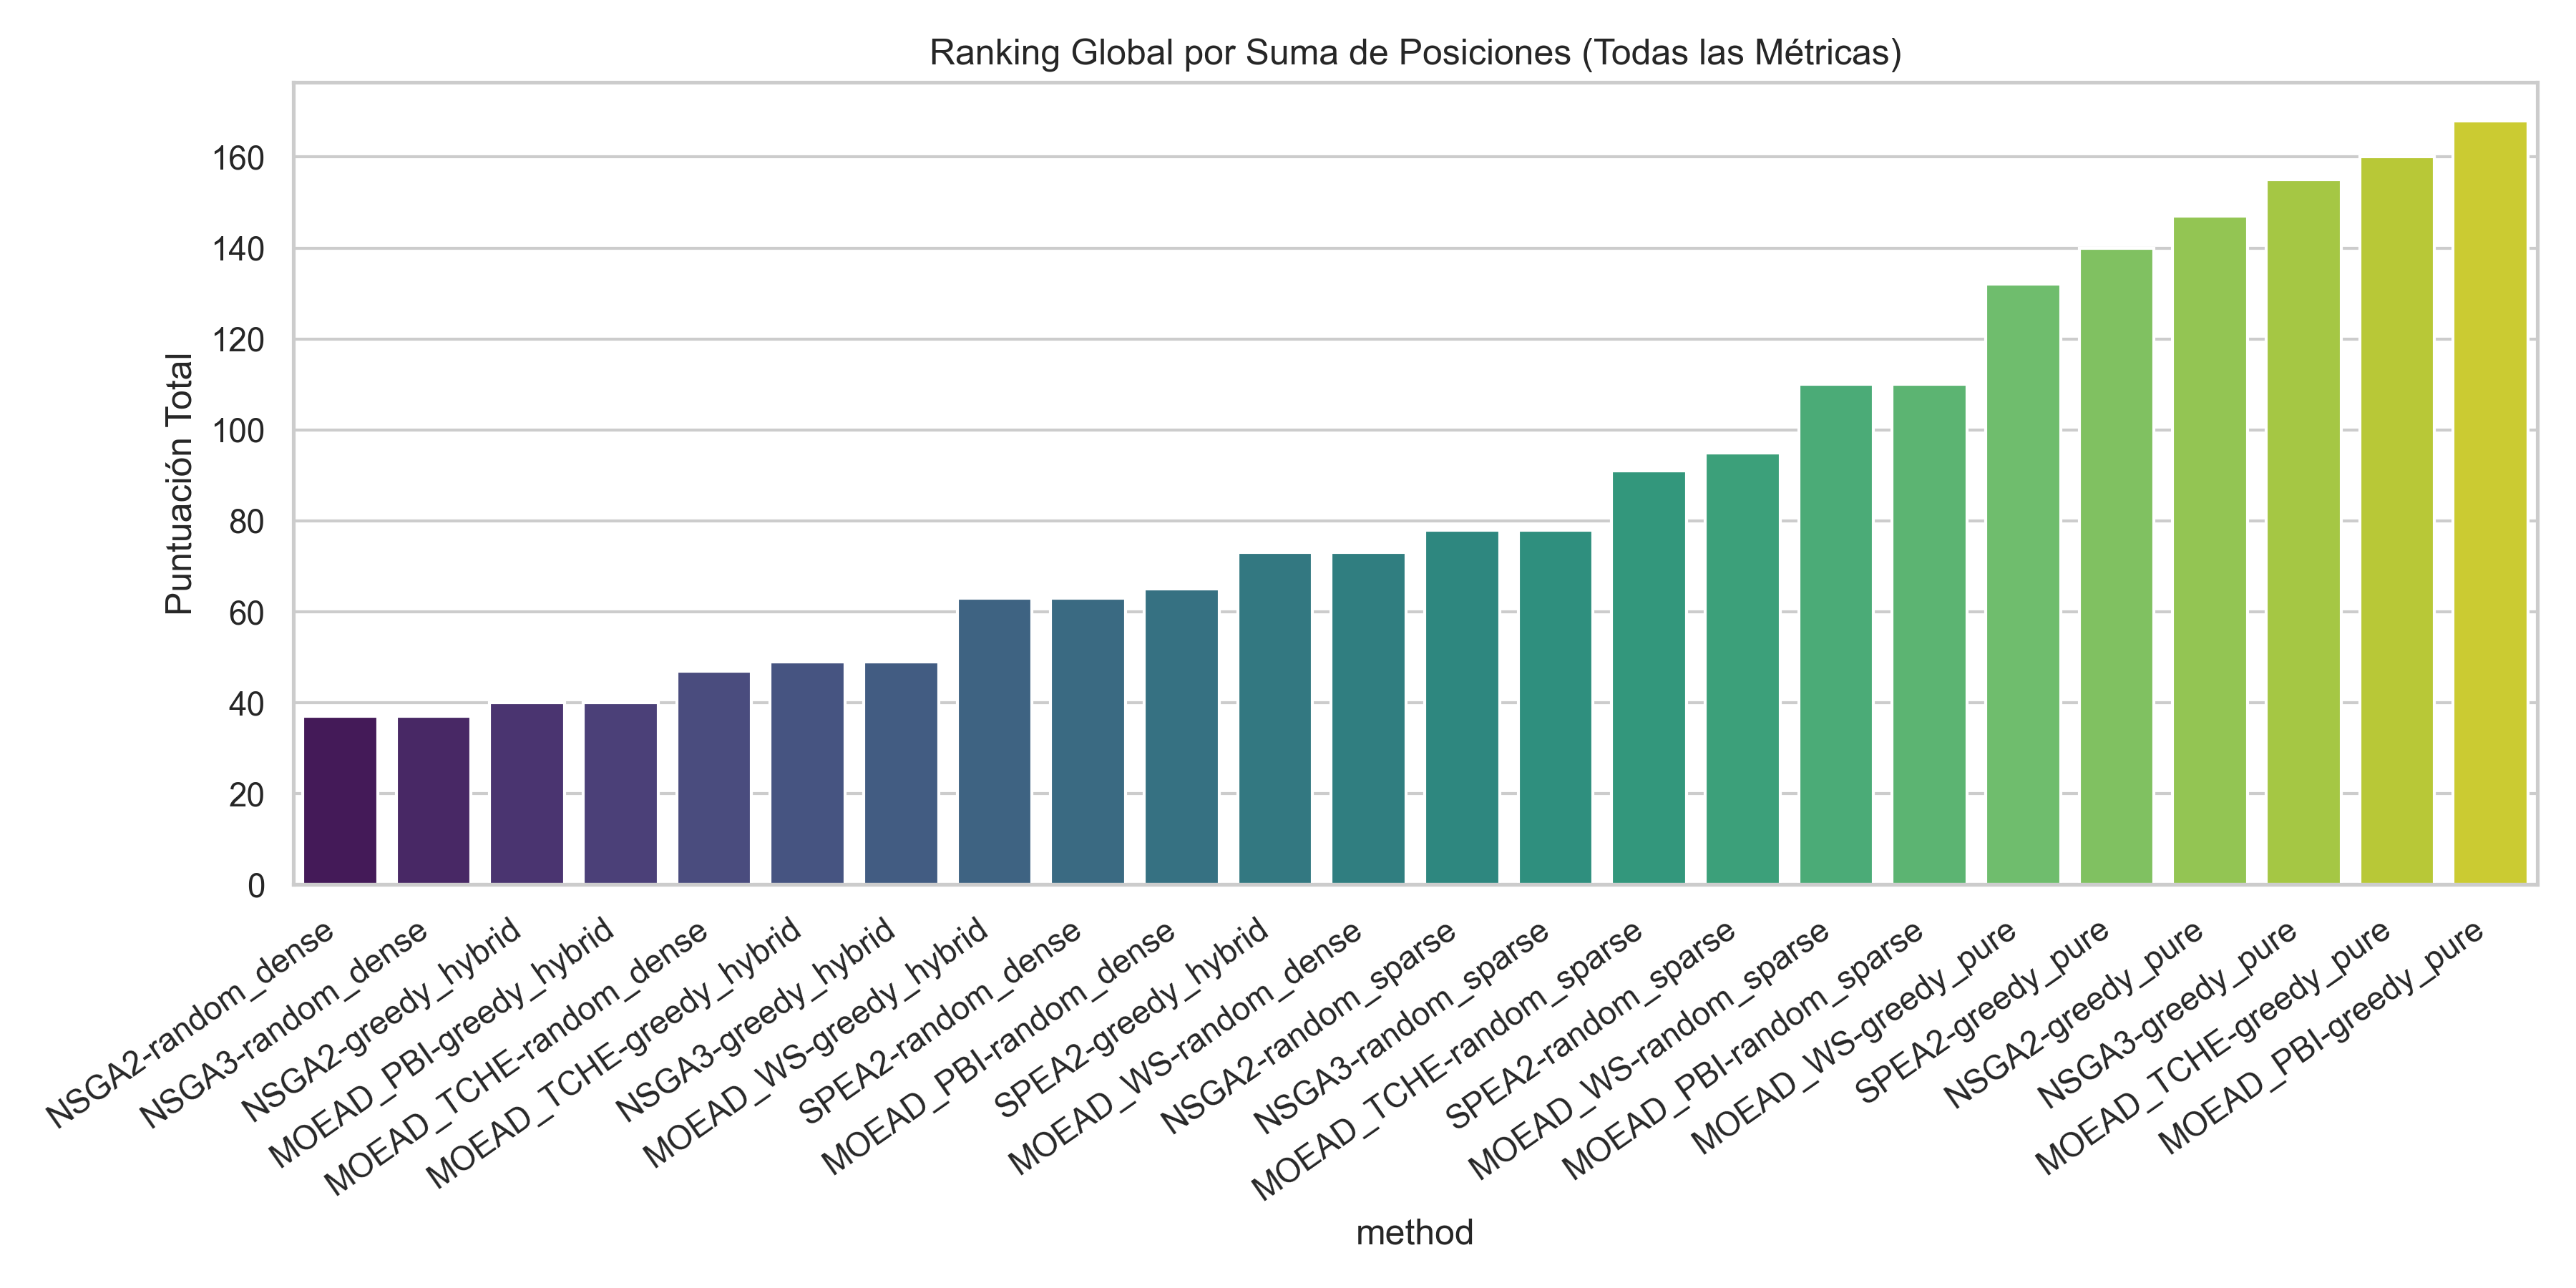
\includegraphics[width=0.6\textwidth]{analisis_assets/20260420T205406/2_comparativa/4_rankings/ranking_global_full.png}
    \caption{Nota sobre el Ranking Global (Rank-Sum): Para evaluar el desempeño de forma equilibrada, se asigna una posición ordinal a cada candidato por métrica. La puntuación global es el sumatorio de estos puestos. Un \textbf{valor menor} indica un desempeño superior y más robusto. \textit{Criterios:} Hypervolume, Range, Tolerance Rate y Hamming ($\uparrow$); SumMin y MinSum ($\downarrow$).}
\end{figure}

\paragraph{Conclusiones (A)}
\begin{itemize}
    \item \textbf{Eficiencia de \texttt{random\_dense}:} El hallazgo más significativo es el liderazgo de la estrategia \texttt{random\_dense} en el ranking global (\textbf{NSGA2} y \textbf{NSGA3} comparten el 1º puesto con 37.0). Esto demuestra que, bajo los criterios de maximización de precisión, una población inicial con alta densidad de SNPs proporciona al algoritmo una base de exploración más rica, permitiéndole alcanzar distancias de Hamming superiores (puestos 2º y 4º) sin sacrificar la convergencia.
    
    \item \textbf{Dualidad de Desempeño (Convergencia vs. Robustez):} Se observa una especialización clara por algoritmos. Mientras que \textbf{NSGA2 + greedy\_hybrid} se consolida como el mejor motor de exploración al liderar de forma absoluta el \textbf{Hipervolumen}, el \textbf{Rango} y la métrica \textbf{SumMin}, el algoritmo \textbf{MOEAD\_PBI + greedy\_hybrid} se erige como el especialista en robustez biológica, ocupando el 1º puesto tanto en \textbf{Avg. Tolerance Rate} como en \textbf{Max. Tolerance Rate}.
    
    \item \textbf{Superioridad de \texttt{greedy\_hybrid}:} La inicialización \texttt{greedy\_hybrid} domina el \textbf{Top 3 de Hipervolumen}. Esto sugiere que el equilibrio entre la explotación dirigida (greedy) y la diversidad estocástica (random) es la configuración óptima para cubrir las zonas de compromiso del frente de Pareto, evitando la convergencia prematura hacia soluciones extremas.
    
    \item \textbf{Degradación por Exceso de Explotación (\textit{Greedy Pure}):} Los datos confirman el fracaso de la estrategia \texttt{greedy\_pure} en este escenario, situándose en la última posición del ranking global (Score: 168.0). La falta de diversidad inicial impide que los algoritmos escapen de óptimos locales, resultando en paneles de SNPs que son superados en todas las dimensiones de calidad por las aproximaciones que incorporan componentes aleatorios.

\end{itemize}


% =========================================================
\subsection{Reporte 3 — Ejecución B: 20260422T113918}
\label{sec:reporte3}

\subsubsection{Configuración}

\paragraph{Configuración resumida (igual que A pero con \textit{inverse})}
\begin{itemize}
    \item \textbf{Infraestructura:} Implementada mediante la librería especializada \textbf{pymoo} (Python).
    \item \textbf{Dataset:} Hinds 2005 (\texttt{hinds2005\_1032.txt}). 772 SNPs polimórficos efectivos.
    \item \textbf{Configuración Global:}
    \begin{itemize}
        \item \textbf{Transformación de objetivos:} Inversión no lineal ($1/f$) para objetivos de maximización ($f_2$ y $f_3$).
        \item \textbf{Normalización:} Escalado estático basado en los límites del conjunto de datos \\ (modo \textbf{\texttt{static\_dataset\_limits}}). Se explica en detalle en la siguiente sección.
    \end{itemize}
    \item \textbf{Parámetros de los Algoritmos:}
    \begin{itemize}
        \item \textbf{Ajustes generales:}
        \begin{itemize}
            \item \textbf{Tamaño de la población:} 200 individuos.
            \item \textbf{Número de generaciones:} 500.
            \item \textbf{Número de descendientes por generación:} 200.
            \item \textbf{Número de ejecuciones independientes:} 5 (para validación estadística).
            \item \textbf{Probabilidad de cruce:} 70\% (Cruce Uniforme).
            \item \textbf{Probabilidad de mutación:} Definida matemáticamente como la inversa de la longitud del cromosoma ($1/L \approx 0,0013$), lo que equivale estadísticamente a la alteración de un único gen por individuo.
        \end{itemize}
        \item \textbf{Ajustes específicos de los algoritmos:}
        \begin{itemize}
            \item \textbf{NSGA-II / SPEA2:} Basados en ordenamiento por dominancia y densidad de soluciones.
            \item \textbf{NSGA-III:} 9 particiones por objetivo para generar un conjunto de 200 direcciones de referencia (Das-Dennis). Se incrementa la densidad de vectores respecto a A para mejorar la resolución.
            \item \textbf{MOEA/D (TCHE, PBI, WS):}
            \begin{itemize}
                \item \textbf{Tamaño del vecindario:} 15 subproblemas.
                \item \textbf{Probabilidad de selección en vecindad:} 90\%.
                \item \textbf{Valor de penalización PBI:} 5.0.
            \end{itemize}
        \end{itemize}
    \end{itemize}
    \item \textbf{Estrategias de Inicialización:}
    \begin{itemize}
        \item \texttt{random\_sparse}: \textbf{Aleatoria Dispersa}. Inicialización con baja densidad de selección (9\% de SNPs activos). Está orientada a descubrir paneles de SNPs muy reducidos y eficientes desde el inicio de la búsqueda.
        \item \texttt{random\_dense}: \textbf{Aleatoria Densa}. Inicialización con alta densidad de selección (50\% de SNPs activos). Su objetivo es evaluar el potencial del algoritmo para simplificar y podar conjuntos de datos con gran cantidad de información redundante.
        \item \texttt{greedy\_pure}: \textbf{Voraz Pura}. Técnica de construcción incremental que asegura la cobertura total de los pares de haplotipos. Garantiza que todos los individuos de la población inicial representen soluciones biológicamente válidas (factibles).
        \item \texttt{greedy\_hybrid}: \textbf{Híbrida Voraz}. Enfoque combinado que alterna entre la lógica voraz y el muestreo aleatorio (proporción 50/50). Persigue un equilibrio óptimo entre la calidad inicial de las soluciones y la diversidad genética necesaria para evitar el estancamiento.
    \end{itemize}
    \item \textbf{Tiempo de ejecución de experimentos:} 1 hora, 15 minutos y 16 segundos para completar el total de 120 ejecuciones individuales.
\end{itemize}

\paragraph{Profundización de la configuración}

\subparagraph{Nota metodológica sobre la comparabilidad}
La Ejecución \textbf{A} utiliza una transformación de objetivos mediante negación (\texttt{neg}), mientras que la Ejecución \textbf{B} emplea inversión (\texttt{inverse}). Por lo tanto, los valores agregados de A y B \textbf{no son comparables directamente por su magnitud bruta}. La comparativa debe centrarse en el \textbf{ranking relativo} de los algoritmos dentro de cada entorno y en los valores decodificados cuando proceda.

\textit{Guía de Comparabilidad:}
\begin{itemize}
    \item \textbf{Métricas NO comparables (en valor absoluto):} No deben compararse cuantitativamente entre A y B debido a que dependen de la topología del espacio transformado.
    \begin{itemize}
        \item \textbf{Hypervolume (HV):} Mide volúmenes en espacios con naturalezas distintas (lineal vs. recíproca).
        \item \textbf{SumMin y MinSum:} Agregados basados en sumas de valores negativos vs. inversos.
        \item \textbf{Range:} La dispersión se ve alterada por la compresión asintótica de la inversión.
    \end{itemize}
    \item \textbf{Métricas SÍ comparables (directamente):} Indicadores robustos que preservan su significado físico o estadístico.
    \begin{itemize}
        \item \textbf{Valores Biológicos Decodificados:} Tasa de Tolerancia real, Distancia de Hamming y número de SNPs.
        \item \textbf{Ranking Relativo y Global Rank-Sum:} La posición ordinal de los algoritmos es una medida universal de desempeño relativo.
        \item \textbf{Tiempo de Ejecución y Cardinalidad:} Medidas de eficiencia y resolución del frente de Pareto.
    \end{itemize}
\end{itemize}

\paragraph{Normalización}
El sistema aplica normalización de objetivos a un espacio $[0, 1]$ para calcular indicadores agregados con el modo \textbf{\texttt{static\_dataset\_limits}}:
\begin{equation}
\label{eq:norm_B}
F_{norm} = \frac{f - f_{ideal}}{f_{nadir} - f_{ideal}}
\end{equation}

\subsubsection{Resultados y análisis (B)}

\paragraph{Frente de Pareto Global}
\begin{figure}[H]
    \centering
    
\includegraphics[width=0.6\textwidth]{analisis_assets/20260422T113918/2_comparativa/1_frentes/frentes_pareto/frentes_pareto_global_full.png}
    \caption{Frente de Pareto Global consolidado para la Ejecución B.}
\end{figure}

\paragraph{Frentes de Pareto (Convergencia final)}

\begin{table}[H]
    \centering
    \begin{tabular}{m{2.2cm} >{\centering\arraybackslash}m{3.2cm} >{\centering\arraybackslash}m{3.2cm} >{\centering\arraybackslash}m{3.2cm} >{\centering\arraybackslash}m{3.2cm}}
        \toprule
        Algoritmo & random\_sparse & random\_dense & greedy\_pure & greedy\_hybrid \\
        \midrule
        \textbf{NSGA-II} & 
\includegraphics[width=\linewidth]{analisis_assets/20260422T113918/2_comparativa/1_frentes/frentes_pareto/frentes_pareto_nsga2_random_sparse_full.png} & 
\includegraphics[width=\linewidth]{analisis_assets/20260422T113918/2_comparativa/1_frentes/frentes_pareto/frentes_pareto_nsga2_random_dense_full.png} & 
\includegraphics[width=\linewidth]{analisis_assets/20260422T113918/2_comparativa/1_frentes/frentes_pareto/frentes_pareto_nsga2_greedy_pure_full.png} & 
\includegraphics[width=\linewidth]{analisis_assets/20260422T113918/2_comparativa/1_frentes/frentes_pareto/frentes_pareto_nsga2_greedy_hybrid_full.png} \\
        \textbf{NSGA-III} & 
\includegraphics[width=\linewidth]{analisis_assets/20260422T113918/2_comparativa/1_frentes/frentes_pareto/frentes_pareto_nsga3_random_sparse_full.png} & 
\includegraphics[width=\linewidth]{analisis_assets/20260422T113918/2_comparativa/1_frentes/frentes_pareto/frentes_pareto_nsga3_random_dense_full.png} & 
\includegraphics[width=\linewidth]{analisis_assets/20260422T113918/2_comparativa/1_frentes/frentes_pareto/frentes_pareto_nsga3_greedy_pure_full.png} & 
\includegraphics[width=\linewidth]{analisis_assets/20260422T113918/2_comparativa/1_frentes/frentes_pareto/frentes_pareto_nsga3_greedy_hybrid_full.png} \\
        \textbf{SPEA2} & 
\includegraphics[width=\linewidth]{analisis_assets/20260422T113918/2_comparativa/1_frentes/frentes_pareto/frentes_pareto_spea2_random_sparse_full.png} & 
\includegraphics[width=\linewidth]{analisis_assets/20260422T113918/2_comparativa/1_frentes/frentes_pareto/frentes_pareto_spea2_random_dense_full.png} & 
\includegraphics[width=\linewidth]{analisis_assets/20260422T113918/2_comparativa/1_frentes/frentes_pareto/frentes_pareto_spea2_greedy_pure_full.png} & 
\includegraphics[width=\linewidth]{analisis_assets/20260422T113918/2_comparativa/1_frentes/frentes_pareto/frentes_pareto_spea2_greedy_hybrid_full.png} \\
        \textbf{MOEA/D (PBI)} & 
\includegraphics[width=\linewidth]{analisis_assets/20260422T113918/2_comparativa/1_frentes/frentes_pareto/frentes_pareto_moead_pbi_random_sparse_full.png} & 
\includegraphics[width=\linewidth]{analisis_assets/20260422T113918/2_comparativa/1_frentes/frentes_pareto/frentes_pareto_moead_pbi_random_dense_full.png} & 
\includegraphics[width=\linewidth]{analisis_assets/20260422T113918/2_comparativa/1_frentes/frentes_pareto/frentes_pareto_moead_pbi_greedy_pure_full.png} & 
\includegraphics[width=\linewidth]{analisis_assets/20260422T113918/2_comparativa/1_frentes/frentes_pareto/frentes_pareto_moead_pbi_greedy_hybrid_full.png} \\
        \textbf{MOEA/D (TCHE)} & 
\includegraphics[width=\linewidth]{analisis_assets/20260422T113918/2_comparativa/1_frentes/frentes_pareto/frentes_pareto_moead_tche_random_sparse_full.png} & 
\includegraphics[width=\linewidth]{analisis_assets/20260422T113918/2_comparativa/1_frentes/frentes_pareto/frentes_pareto_moead_tche_random_dense_full.png} & 
\includegraphics[width=\linewidth]{analisis_assets/20260422T113918/2_comparativa/1_frentes/frentes_pareto/frentes_pareto_moead_tche_greedy_pure_full.png} & 
\includegraphics[width=\linewidth]{analisis_assets/20260422T113918/2_comparativa/1_frentes/frentes_pareto/frentes_pareto_moead_tche_greedy_hybrid_full.png} \\
        \textbf{MOEA/D (WS)} & 
\includegraphics[width=\linewidth]{analisis_assets/20260422T113918/2_comparativa/1_frentes/frentes_pareto/frentes_pareto_moead_ws_random_sparse_full.png} & 
\includegraphics[width=\linewidth]{analisis_assets/20260422T113918/2_comparativa/1_frentes/frentes_pareto/frentes_pareto_moead_ws_random_dense_full.png} & 
\includegraphics[width=\linewidth]{analisis_assets/20260422T113918/2_comparativa/1_frentes/frentes_pareto/frentes_pareto_moead_ws_greedy_pure_full.png} & 
\includegraphics[width=\linewidth]{analisis_assets/20260422T113918/2_comparativa/1_frentes/frentes_pareto/frentes_pareto_moead_ws_greedy_hybrid_full.png} \\
        \bottomrule
    \end{tabular}
    \caption{Galería de Frentes de Pareto (B)}
\end{table}

\paragraph{Convergencia Progresiva (B)}
\begin{figure}[H]
    \centering
    \begin{subfigure}[b]{0.40\textwidth}
        
\includegraphics[width=\textwidth]{analisis_assets/20260422T113918/2_comparativa/2_metricas_convergencia/convergencia_range_full.png}
        \caption{Range}
    \end{subfigure}
    \hfill
    \begin{subfigure}[b]{0.40\textwidth}
        
\includegraphics[width=\textwidth]{analisis_assets/20260422T113918/2_comparativa/2_metricas_convergencia/convergencia_summin_full.png}
        \caption{SumMin}
    \end{subfigure}

    \vspace{0.3cm}

    \begin{subfigure}[b]{0.40\textwidth}
        
\includegraphics[width=\textwidth]{analisis_assets/20260422T113918/2_comparativa/2_metricas_convergencia/convergencia_minsum_full.png}
        \caption{MinSum}
    \end{subfigure}
    \hfill
    \begin{subfigure}[b]{0.40\textwidth}
        
\includegraphics[width=\textwidth]{analisis_assets/20260422T113918/2_comparativa/2_metricas_convergencia/convergencia_maxtolerancerate_full.png}
        \caption{Max. Tolerance Rate}
    \end{subfigure}

    \vspace{0.3cm}

    \begin{subfigure}[b]{0.40\textwidth}
        
\includegraphics[width=\textwidth]{analisis_assets/20260422T113918/2_comparativa/2_metricas_convergencia/convergencia_avgtolerancerate_full.png}
        \caption{Avg. Tolerance Rate}
    \end{subfigure}
    \hfill
    \begin{subfigure}[b]{0.40\textwidth}
        
\includegraphics[width=\textwidth]{analisis_assets/20260422T113918/2_comparativa/2_metricas_convergencia/convergencia_avghammingdistance_full.png}
        \caption{Avg Hamming}
    \end{subfigure}

    \vspace{0.3cm}

    \begin{subfigure}[b]{0.40\textwidth}
        
\includegraphics[width=\textwidth]{analisis_assets/20260422T113918/2_comparativa/2_metricas_convergencia/convergencia_hypervolume_full.png}
        \caption{Hypervolume}
    \end{subfigure}
    \caption{Galería de Convergencia (Ejecución B)}
\end{figure}

\paragraph{Top 10 por Métrica (B)}

\begin{table}[H]
    \centering
    \begin{subtable}[t]{0.45\textwidth}
        \centering
        \caption{Range ($\uparrow$)}
        \begin{tabular}{lllc}
            \toprule
            Pos & Algo & Init & Valor \\
            \midrule
            1 & NSGA2 & GH & 2.1878 \\
            2 & MOEAD\_WS & GH & 1.9151 \\
            3 & SPEA2 & GH & 1.8631 \\
            4 & MOEAD\_TCHE & GH & 1.8329 \\
            5 & NSGA2 & RS & 1.5094 \\
            6 & SPEA2 & RS & 1.3274 \\
            7 & MOEAD\_WS & GP & 1.1328 \\
            8 & NSGA3 & GH & 1.1263 \\
            9 & NSGA3 & RS & 1.1047 \\
            10 & NSGA2 & GP & 1.0464 \\
            \bottomrule
        \end{tabular}
    \end{subtable}
    \hfill
    \begin{subtable}[t]{0.45\textwidth}
        \centering
        \caption{SumMin ($\downarrow$)}
        \begin{tabular}{lllc}
            \toprule
            Pos & Algo & Init & Valor \\
            \midrule
            1 & NSGA2 & GH & 0.0168 \\
            2 & MOEAD\_WS & GH & 0.0261 \\
            3 & MOEAD\_TCHE & GH & 0.0290 \\
            4 & SPEA2 & GH & 0.0326 \\
            5 & NSGA2 & RS & 0.0366 \\
            6 & SPEA2 & RS & 0.0645 \\
            7 & MOEAD\_TCHE & RS & 0.0817 \\
            8 & MOEAD\_WS & RS & 0.0922 \\
            9 & NSGA3 & GH & 0.1267 \\
            10 & MOEAD\_PBI & GH & 0.1399 \\
            \bottomrule
        \end{tabular}
    \end{subtable}
\end{table}

\begin{table}[H]
    \centering
    \begin{subtable}[t]{0.45\textwidth}
        \centering
        \caption{MinSum ($\downarrow$)}
        \begin{tabular}{lllc}
            \toprule
            Pos & Algo & Init & Valor \\
            \midrule
            1 & MOEAD\_WS & GH & 0.1697 \\
            2 & MOEAD\_TCHE & RS & 0.1771 \\
            3 & MOEAD\_TCHE & GH & 0.1774 \\
            4 & MOEAD\_WS & RS & 0.1783 \\
            5 & NSGA2 & RS & 0.1819 \\
            6 & MOEAD\_PBI & RS & 0.1830 \\
            7 & NSGA2 & GH & 0.1901 \\
            8 & MOEAD\_PBI & GH & 0.1930 \\
            9 & NSGA3 & GH & 0.1954 \\
            10 & NSGA3 & RS & 0.2019 \\
            \bottomrule
        \end{tabular}
    \end{subtable}
    \hfill
    \begin{subtable}[t]{0.45\textwidth}
        \centering
        \caption{Max. Tolerance Rate ($\uparrow$)}
        \begin{tabular}{lllc}
            \toprule
            Pos & Algo & Init & Valor \\
            \midrule
            1 & MOEAD\_WS & GH & 0.2760 \\
            2 & MOEAD\_TCHE & GH & 0.2541 \\
            3 & MOEAD\_TCHE & RS & 0.2540 \\
            4 & NSGA3 & RD & 0.2476 \\
            5 & NSGA2 & RS & 0.2466 \\
            6 & MOEAD\_WS & RS & 0.2457 \\
            7 & MOEAD\_PBI & RS & 0.2326 \\
            8 & NSGA2 & RD & 0.2300 \\
            9 & NSGA3 & GH & 0.2283 \\
            10 & NSGA2 & GH & 0.2274 \\
            \bottomrule
        \end{tabular}
    \end{subtable}
\end{table}

\begin{table}[H]
    \centering
    \begin{subtable}[t]{0.45\textwidth}
        \centering
        \caption{Avg. Tolerance Rate ($\uparrow$)}
        \begin{tabular}{lllc}
            \toprule
            Pos & Algo & Init & Valor \\
            \midrule
            1 & MOEAD\_PBI & RS & 0.2137 \\
            2 & MOEAD\_WS & GH & 0.2118 \\
            3 & NSGA3 & RD & 0.2105 \\
            4 & NSGA2 & RD & 0.2088 \\
            5 & MOEAD\_TCHE & RS & 0.2022 \\
            6 & MOEAD\_WS & RS & 0.1998 \\
            7 & MOEAD\_TCHE & GH & 0.1921 \\
            8 & MOEAD\_PBI & GH & 0.1822 \\
            9 & MOEAD\_TCHE & RD & 0.1817 \\
            10 & MOEAD\_PBI & RD & 0.1741 \\
            \bottomrule
        \end{tabular}
    \end{subtable}
    \hfill
    \begin{subtable}[t]{0.45\textwidth}
        \centering
        \caption{Avg. Hamming ($\uparrow$)}
        \begin{tabular}{lllc}
            \toprule
            Pos & Algo & Init & Valor \\
            \midrule
            1 & NSGA2 & RD & 127.80 \\
            2 & NSGA3 & RD & 115.97 \\
            3 & SPEA2 & RD & 110.31 \\
            4 & MOEAD\_TCHE & RD & 93.30 \\
            5 & MOEAD\_PBI & RD & 88.99 \\
            6 & MOEAD\_WS & RD & 83.97 \\
            7 & NSGA2 & GH & 74.09 \\
            8 & SPEA2 & GH & 56.24 \\
            9 & NSGA2 & RS & 35.75 \\
            10 & MOEAD\_TCHE & GH & 34.42 \\
            \bottomrule
        \end{tabular}
    \end{subtable}
\end{table}

\begin{table}[H]
    \centering
    \caption{Hypervolume ($\uparrow$)}
    \begin{tabular}{lllc}
        \toprule
        Pos & Algoritmo & Inicialización & Valor \\
        \midrule
        1 & NSGA2 & greedy\_hybrid & 0.9501 \\
        2 & MOEAD\_WS & greedy\_hybrid & 0.9435 \\
        3 & NSGA2 & random\_sparse & 0.9410 \\
        4 & SPEA2 & greedy\_hybrid & 0.9383 \\
        5 & MOEAD\_TCHE & greedy\_hybrid & 0.9378 \\
        6 & SPEA2 & random\_sparse & 0.9185 \\
        7 & MOEAD\_TCHE & random\_sparse & 0.9125 \\
        8 & MOEAD\_WS & random\_sparse & 0.9044 \\
        9 & NSGA3 & greedy\_hybrid & 0.8689 \\
        10 & MOEAD\_PBI & greedy\_hybrid & 0.8644 \\
        \bottomrule
    \end{tabular}
\end{table}

\paragraph{Correlación de Métricas (Heatmap)}
\begin{figure}[H]
    \centering
    
\includegraphics[width=0.6\textwidth]{analisis_assets/20260422T113918/2_comparativa/4_rankings/heatmap_comparativa_full.png}
    \caption{Comparativa de métricas para la Ejecución B.}
\end{figure}

\paragraph{Ranking Global (Rank-Sum)}
\begin{figure}[H]
    \centering
    
\includegraphics[width=0.6\textwidth]{analisis_assets/20260422T113918/2_comparativa/4_rankings/ranking_global_full.png}
    \caption{Nota sobre el Ranking Global (Rank-Sum): Para evaluar el desempeño de forma equilibrada, se asigna una posición ordinal a cada candidato por métrica. La puntuación global es el sumatorio de estos puestos. Un \textbf{valor menor} indica un desempeño superior y más robusto. \textit{Criterios:} Hypervolume, Range, Tolerance Rate y Hamming ($\uparrow$); SumMin y MinSum ($\downarrow$).}
\end{figure}

\paragraph{Conclusiones (B)}
\begin{itemize}
    \item \textbf{Liderazgo Indiscutible:} \textbf{MOEAD\_WS + greedy\_hybrid} se posiciona como la configuración ganadora absoluta (Score: 22.0), liderando la métrica de \textbf{MinSum} y situándose en el Top 2 de \textbf{Hipervolumen, Rango y Max. Tolerance Rate}.
    \item \textbf{Exploración y Diversidad:} \textbf{NSGA2 + greedy\_hybrid} mantiene el liderazgo en \textbf{Hipervolumen} (0.9501) y \textbf{Rango}, consolidándose como el motor de búsqueda más potente para cubrir el frente de Pareto.
    \item \textbf{Especialización en Hamming:} La inicialización \textbf{random\_dense} maximiza la distancia de Hamming (distinción genética), con \textbf{NSGA2} a la cabeza de esta métrica.
    \item \textbf{Efectividad Híbrida:} La estrategia \texttt{greedy\_hybrid} domina el Top 3 global, demostrando que el equilibrio entre exploración aleatoria y explotación dirigida es clave para optimizar simultáneamente convergencia y robustez.
\end{itemize}


\section{Comparación Final (Moqa vs A vs B)}

\end{document}
